\documentclass{createspace}
\newcommand{\N}{\mathbb N}
\newcommand{\Z}{\mathbb Z}
\newcommand{\Q}{\mathbb Q}
\newcommand{\R}{\mathbb R}
\newcommand{\C}{\mathbb C}

\newcommand{\shrap}{\mathbin{\#}}
\DeclareMathOperator*{\bigshrap}{\#}

\newcommand{\bracket}[1]{\left\langle{#1}\right\rangle}

\newcommand{\alexander}{\Delta}
\newcommand{\conway}{\nabla}
\newcommand{\jones}{V}
% span?

\newcommand{\braid}{\operatorname{b}}
\newcommand{\bridge}{\operatorname{br}}
\newcommand{\crossing}{\operatorname{cr}}
\newcommand{\genus}{\operatorname{g}}
\newcommand{\linking}{\operatorname{lk}}
\newcommand{\sign}{\operatorname{sgn}}
\newcommand{\volume}{\operatorname{vol}}
\newcommand{\writhe}{\operatorname{wr}}


\usepackage{enumitem}
\usepackage{booktabs}
\usepackage{longtable}
\usepackage[table]{xcolor}
\usepackage[colorinlistoftodos,prependcaption]{todonotes}
\usepackage{tikz}
\usetikzlibrary{arrows.meta}
\usetikzlibrary{decorations.markings}
\usetikzlibrary{decorations.pathreplacing}
\usetikzlibrary{knots}
\colorlet{darkblue}{blue!80!black}
\newcommand{\MalyNieWezel} {\begin{tikzpicture}[baseline=-0.65ex, scale=0.02]
	\begin{knot}[clip width=5, end tolerance=1pt]
		\strand[semithick] (0,0) circle (5);
	\end{knot}
\end{tikzpicture}}

\newcommand{\NieWezel} {\begin{tikzpicture}[baseline=-0.65ex, scale=0.04]
	\begin{knot}[clip width=5, end tolerance=1pt]
		\strand[semithick] (0,0) circle (5);
	\end{knot}
\end{tikzpicture}}

\newcommand{\PrawyKrzyz} {\begin{tikzpicture}[baseline=-0.65ex, scale=0.04]
	\useasboundingbox (-5, -5) rectangle (5,5);
	\begin{knot}[clip width=5, end tolerance=1pt, flip crossing/.list={1}] 
		\strand[semithick] (-5,5) to (5,-5);
		\strand[semithick] (-5,-5) to (5,5);
	\end{knot}
\end{tikzpicture}}

\newcommand{\MalyPrawyGladki} {
	\begin{tikzpicture}[baseline=-0.65ex,scale=0.03]
	\begin{knot}[clip width=5, end tolerance=1pt] 
		\strand[semithick] (-4, -5) to [out=45, in=-45] (-4, 5);
		\strand[semithick] (4, -5) to [out=135, in=-135] (4, 5);
	\end{knot}
	\end{tikzpicture}
}

\newcommand{\MalyPrawyKrzyz} {\begin{tikzpicture}[baseline=-0.65ex, scale=0.03]
	\useasboundingbox (-5, -5) rectangle (5,5);
	\begin{knot}[clip width=5, end tolerance=1pt, flip crossing/.list={1}] 
		\strand[semithick] (-5,5) to (5,-5);
		\strand[semithick] (-5,-5) to (5,5);
	\end{knot}
\end{tikzpicture}}

\newcommand{\PrawyGladkiKreslony} {
	\begin{tikzpicture}[baseline=-0.65ex,yscale=0.07, xscale=0.1]
	\useasboundingbox (-5, -6) rectangle (5, 6);
	\begin{knot}[clip width=5, end tolerance=1pt] 
		\strand[semithick] (-4, -5) to [out=45, in=-45] (-4, 5);
		\strand[semithick] (4, -5) to [out=135, in=-135] (4, 5);
		\strand[semithick] (-5, 0) to (5, 0);
	\end{knot}
	\end{tikzpicture}
}

\newcommand{\LewyGladkiKreslony} {
	\begin{tikzpicture}[baseline=-0.65ex,yscale=0.07, xscale=0.1]
	\useasboundingbox (-5, -6) rectangle (5, 6);
	\begin{knot}[clip width=5, end tolerance=1pt] 
		\strand[semithick] (-5, 5) [in=-135, out=-45] to (5,5);
		\strand[semithick] (-5, -5) [in=135, out=45] to (5,-5);
		\strand[semithick] (-5, 0) to (5, 0);
	\end{knot}
	\end{tikzpicture}
}

\newcommand{\LewyKrzyz} {\begin{tikzpicture}[scale=0.03, baseline=-3]
	\begin{knot}[clip width=5, end tolerance=1pt] 
		\strand[semithick] (-5,5) to (5,-5);
		\strand[semithick] (-5,-5) to (5,5);
	\end{knot}
\end{tikzpicture}}

\newcommand{\MalyLewyGladki} {
	\begin{tikzpicture}[baseline=-0.65ex,scale=0.03]
	\begin{knot}[clip width=5, end tolerance=1pt] 
		\strand[semithick] (-5, 5) [in=-135, out=-45] to (5,5);
		\strand[semithick] (-5, -5) [in=135, out=45] to (5,-5);
	\end{knot}
	\end{tikzpicture}
}

\newcommand{\MalyLewyKrzyz} {
	\begin{tikzpicture}[baseline=-0.65ex,scale=0.03]
	\begin{knot}[clip width=5, end tolerance=1pt] 
		\strand[semithick] (-5, -5) to [out=up, in=up] (5, -5);
		\strand[semithick] (-5, 5) to [out=down, in=down] (5, 5);
	\end{knot}
	\end{tikzpicture}
}

\newcommand{\reidemeisterIa} {
\begin{tikzpicture}[baseline=-0.65ex, scale=0.07]
\useasboundingbox (-4, -5) rectangle (3, 5);
\begin{knot}[clip width=5, end tolerance=1pt] 
	\strand[semithick] (-3,  5) [in=left, out=down] to (1, -2) [in=down, out=right] to (3, 0);
	\strand[semithick] (-3, -5) [in=left, out=up]   to (1,  2) [in=up,   out=right] to (3, 0);
\end{knot}
\end{tikzpicture}
}

\newcommand{\MalyreidemeisterIa} {\begin{tikzpicture}[baseline=-0.65ex, scale=0.03]
\useasboundingbox (-4, -5) rectangle (3, 5);
\begin{knot}[clip width=5, end tolerance=1pt] 
	\strand[semithick] (-3,  5) [in=left, out=down] to (1, -2) [in=down, out=right] to (3, 0);
	\strand[semithick] (-3, -5) [in=left, out=up]   to (1,  2) [in=up,   out=right] to (3, 0);
	\end{knot}
	\end{tikzpicture}}

\newcommand{\MalyreidemeisterIb} {\begin{tikzpicture}[baseline=-0.65ex, scale=0.03]
	\begin{knot}[clip width=5, end tolerance=1pt] 
		\strand[semithick] (0,-5) to (0, 5);
	\end{knot}
\end{tikzpicture}}

\newcommand{\reidemeisterIb} {
\begin{tikzpicture}[baseline=-0.65ex, scale=0.07]
\begin{knot}[clip width=5, end tolerance=1pt] 
	\strand[semithick] (0,-5) to (0, 5);
\end{knot}
\end{tikzpicture}
}

% potrzebne do klamry Kauffmana
\newcommand{\reidemeisterIab} {
\begin{tikzpicture}[baseline=-0.65ex,scale=0.07]
\useasboundingbox (-5, -6) rectangle (5, 6);
\begin{knot}[clip width=5, end tolerance=1pt] 
	\strand[semithick] (4,-5) .. controls (4,-3) and (-4,-3) .. (-4,-1);
	\strand[semithick] (-4,-5) .. controls (-4,-3) and (4,-3) .. (4,-1);
	\strand[semithick] (-4,-1) [in=left, out=up] to (0, 1) to [in=up, out=right] (4,-1);
	\strand[semithick] (-4, 5) [in=left, out=down] to (0, 3) to [in=down, out=right] (4, 5);
\end{knot}
\end{tikzpicture}
}

\newcommand{\reidemeisterIIa} {
\begin{tikzpicture}[baseline=-0.65ex,scale=0.07]
\useasboundingbox (-5, -6) rectangle (5, 6);
\begin{knot}[clip width=5, end tolerance=1pt] 
	\strand[semithick] (4,-5) .. controls (4,-2) and (-4,-2) .. (-4,0);
	\strand[semithick] (4,5) .. controls (4, 2) and (-4, 2) .. (-4,0);
	\strand[semithick] (-4,-5) .. controls (-4,-2) and (4,-2) .. (4,0);
	\strand[semithick] (-4,5) .. controls (-4, 2) and (4,2) .. (4,0);
\end{knot}
\end{tikzpicture}
}

% reidemeister II a poziomo
\newcommand{\reidemeisterIIaa} {
\begin{tikzpicture}[baseline=-0.65ex,scale=0.05]
\begin{knot}[clip width=5, end tolerance=1pt] 
	\strand[semithick] (-10, -5) to [out=right, in=left] ( 0,  5) 
	                             to [out=right, in=left] (10, -5);
	\strand[semithick] (-10,  5) to [out=right, in=left] ( 0, -5) 
	                             to [out=right, in=left] (10,  5);
\end{knot}
\end{tikzpicture}
}

\newcommand{\reidemeisterIIb} {
\begin{tikzpicture}[baseline=-0.65ex,scale=0.07]
\begin{knot}[clip width=5, end tolerance=1pt] 
	\strand[semithick] (4,-5) .. controls (4,-2) and (1,-2) .. (1,0);
	\strand[semithick] (4,5) .. controls (4, 2) and (1, 2) .. (1,0);
	\strand[semithick] (-4,-5) .. controls (-4,-2) and (-1,-2) .. (-1,0);
	\strand[semithick] (-4,5) .. controls (-4, 2) and (-1,2) .. (-1,0);
\end{knot}
\end{tikzpicture}
}

\newcommand{\reidemeisterIIIa} {
\begin{tikzpicture}[baseline=-0.65ex,yscale=0.07, xscale=0.1]
\useasboundingbox (-5, -6) rectangle (5, 6);
\begin{knot}[clip width=5, flip crossing/.list={1,2,3}, end tolerance=1pt] 
	\strand[semithick] (-5,-5) -- (5,5);
	\strand[semithick] (-5,5) -- (5,-5);
	\strand[semithick] (-5,-1) .. controls (-2, -1) and (-2,4) .. (0,4) .. controls (2, 4) and (2, -1) .. (5, -1);
\end{knot}
\end{tikzpicture}
}

\newcommand{\reidemeisterIIIb} {
\begin{tikzpicture}[baseline=-0.65ex,yscale=0.07, xscale=0.1]
\useasboundingbox (-5, -6) rectangle (5, 6);
\begin{knot}[clip width=5, flip crossing/.list={1,2,3}, end tolerance=1pt] 
	\strand[semithick] (-5,-5) -- (5,5);
	\strand[semithick] (-5,5) -- (5,-5);
	\strand[semithick](-5,+1) .. controls (-2,+1) and (-2,-4) .. (0,-4) .. controls (2,-4) and (2,+1) .. (5,+1);
\end{knot}
\end{tikzpicture}
}

\newcommand{\skeinplus} {
\begin{tikzpicture}[baseline=-0.65ex,scale=0.1]
\useasboundingbox (-5, -6) rectangle (5, 6);
\begin{knot}[clip width=5, end tolerance=1pt] 
	\strand[semithick,-latex] (-5, -5) to (5,  5);
	\strand[semithick,latex-] (-5,  5) to (5, -5);
	\node[darkblue] at (0,-4)[below] {$L_+$};
\end{knot}
\end{tikzpicture}
}

\newcommand{\skeinminus} {
\begin{tikzpicture}[baseline=-0.65ex,scale=0.1]
\useasboundingbox (-5, -6) rectangle (5, 6);
\begin{knot}[clip width=5, end tolerance=1pt, flip crossing/.list={1}] 
	\strand[semithick,-latex] (-5, -5) to (5,  5);
	\strand[semithick,latex-] (-5,  5) to (5, -5);
	\node[darkblue] at (0,-4)[below] {$L_-$};
\end{knot}
\end{tikzpicture}
}

\newcommand{\skeinzero} {
\begin{tikzpicture}[baseline=-0.65ex,scale=0.1]
\useasboundingbox (-5, -6) rectangle (5, 6);
\begin{knot}[clip width=5, end tolerance=1pt, flip crossing/.list={1}] 
	\strand[semithick,-latex] (-5, -5) to [out=45, in=-45] (-5, 5);
	\strand[semithick,-Latex] (5, -5) to [out=135, in=-135] (5, 5);
	\node[darkblue] at (0,-4)[below] {$L_0$};
\end{knot}
\end{tikzpicture}
}

\tikzset{
	->-/.style={decoration={markings, mark=at position .5 with {\arrow{>}}},postaction={decorate}},
	-<-/.style={decoration={markings, mark=at position .5 with {\arrow{<}}},postaction={decorate}},
	LUK/.style ={
		draw=black,
		line join=miter,
		line cap=butt,
		miter limit=4.00,
		line width=0.2 mm
	},
	CIENKILUK/.style ={
		draw=black,
		line join=miter,
		line cap=butt,
		miter limit=4.00,
		line width=0.1 mm
	},
	TEKSTOWY/.style ={
		draw=black,
		line join=round,
		line cap=butt,
		miter limit=20.00,
		line width=0.2 mm
	},
	OBSZAR/.style={
		draw=none,
		fill=white!#1!red
	},
	OBSZAR/.default = 80,
}

\author{Leon Suwalski}
\title{Krótkie wprowadzenie do teorii węzłów}
\date{2018}

\begin{document}
\maketitle
\tableofcontents
\chapter{Preludium}
\label{cha:preludium}
Teoria węzłów to gałąź topologii,
która powstała z~inspiracji węzłami,
jakie pojawiają się w~codziennym życiu: przy wiązaniu butów albo cumowaniu statków.
Zajmuje się ona badaniem przede wszystkim węzłów,
czyli pewnych włożeń okręgu $S^1$ w~trójwymiarową przestrzeń euklidesową $\R^3$ lub sferę $S^3$,
ale także splotów (zaplątanych w~sobie węzłów), warkoczy, supłów oraz podobnych obiektów.
Matematyczne węzły różnią się tym od zwykłych, że ich końce są ze sobą połączone.

Oto kilka przykładów.
Węzeł (a) nazywamy niewęzłem, jest to kalka angielskiego \emph{unknot}.
Następne w~kolejce widoczne są trójlistnik (b,~\emph{trefoil}), ósemka (c,~\emph{figure-eight}), pięciolistnik (d,~\emph{cinquefoil}) oraz słynna para Perko (e,~f~wg oryginalnej numeracji Rolfsena).
Pod diagramami umieściliśmy notację Alexandera-Briggsa, jeszcze do niej wrócimy.

\begin{figure}[H]
    \centering
    \begin{minipage}[b]{.14\linewidth}
        \centering
        $\begin{tikzpicture}[baseline=-0.65ex, scale=0.5] \begin{knot}[clip width=5, end tolerance=1pt] \strand[semithick] (0,0) circle (\linewidth); \end{knot}
\end{tikzpicture}$
        \subcaption{}
    \end{minipage}
    \begin{minipage}[b]{.14\linewidth}
        \centering
        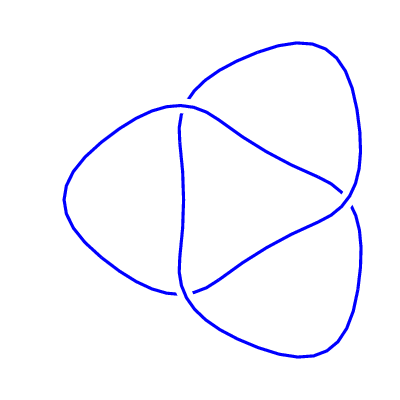
\includegraphics[width=\linewidth]{../data/3_1.png}
        \subcaption{$3_1$}
    \end{minipage}
    \begin{minipage}[b]{.14\linewidth}
        \centering
        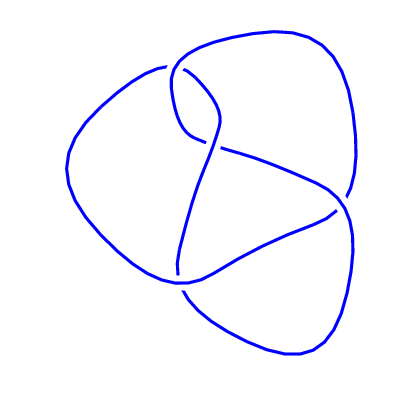
\includegraphics[width=\linewidth]{../data/4_1.png}
        \subcaption{$4_1$}
    \end{minipage}
    \begin{minipage}[b]{.14\linewidth}
        \centering
        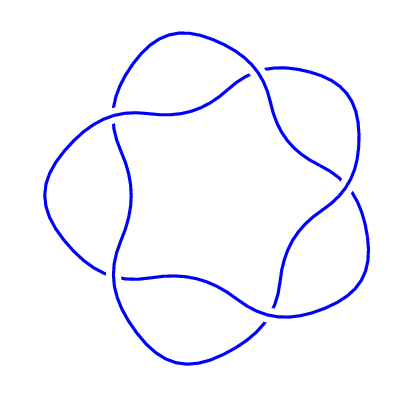
\includegraphics[width=\linewidth]{../data/5_1.png}
        \subcaption{$5_1$}
    \end{minipage}
    \begin{minipage}[b]{.14\linewidth}
        \centering
        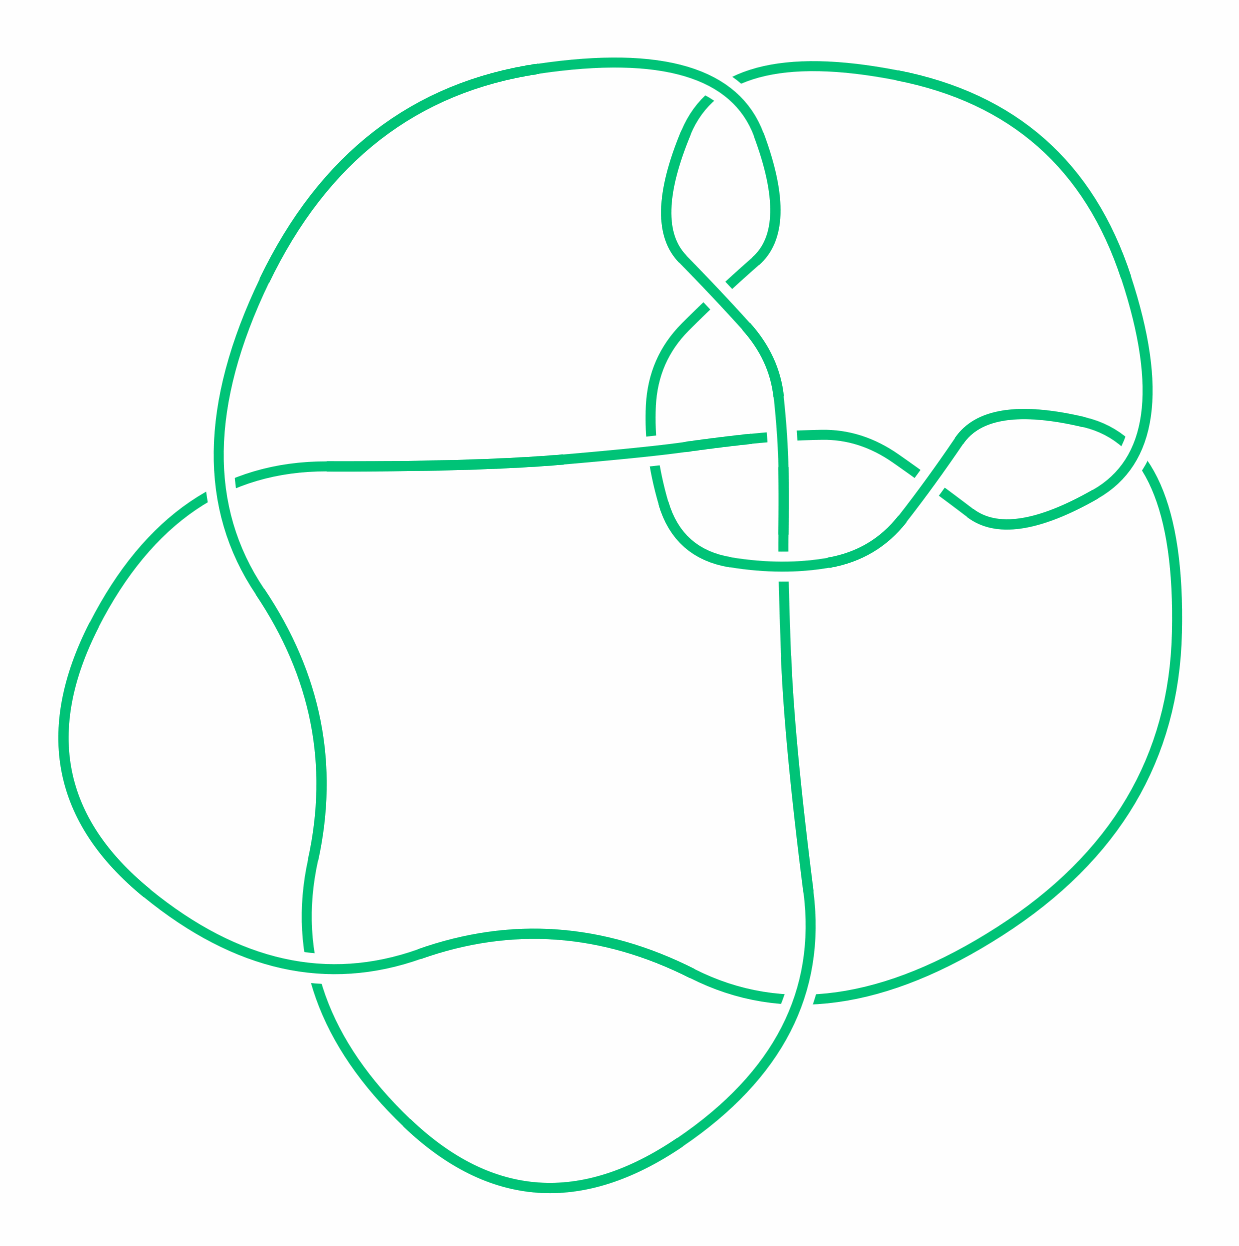
\includegraphics[width=\linewidth]{../data/perko1.png}
        \subcaption{$10_{161}$}
    \end{minipage}
    \begin{minipage}[b]{.14\linewidth}
        \centering
        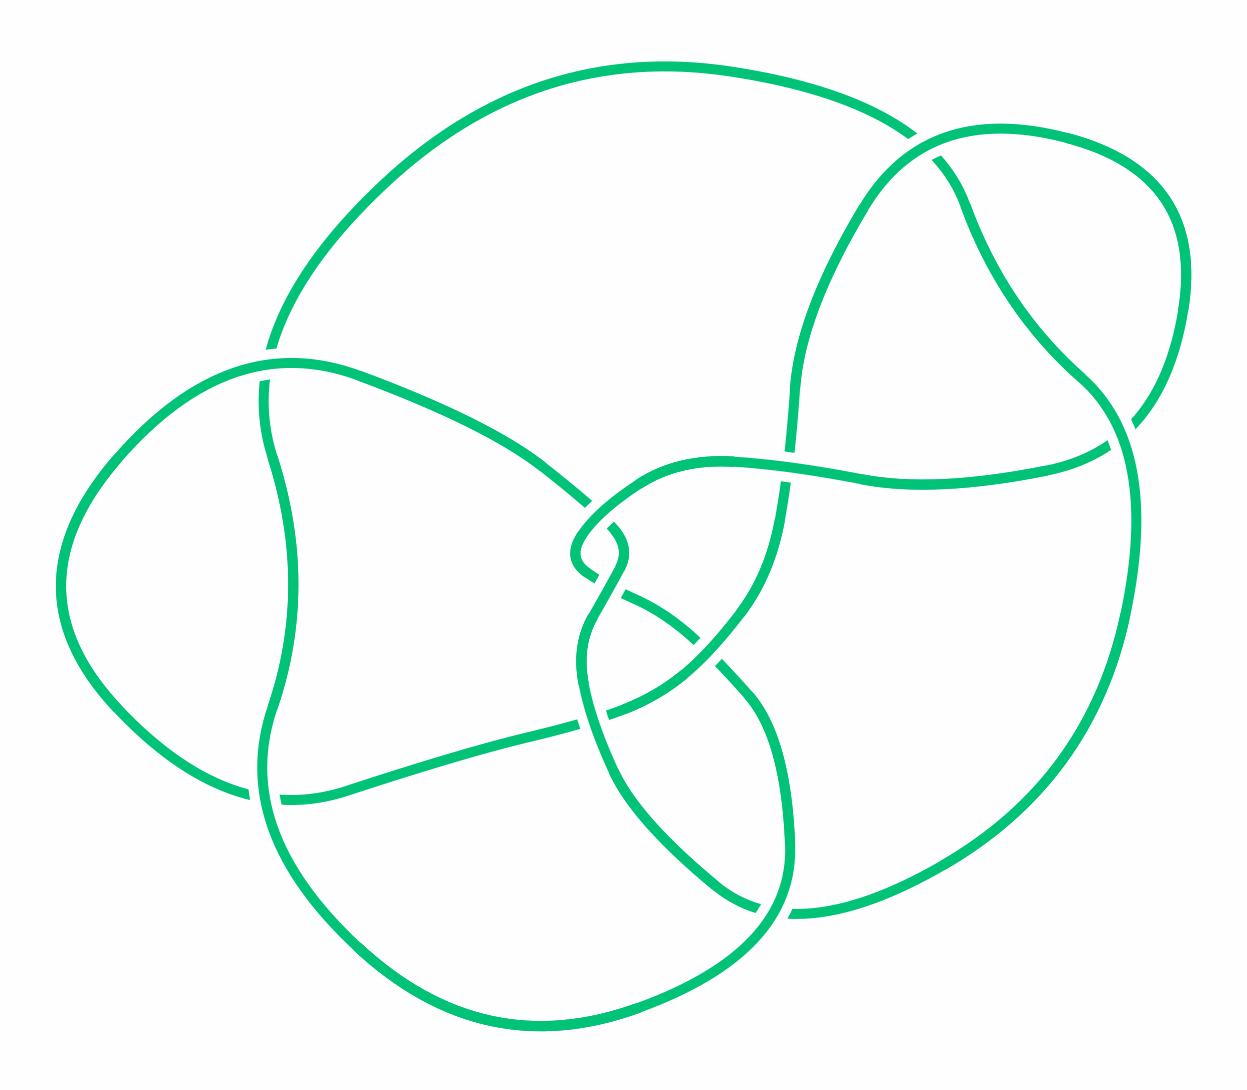
\includegraphics[width=\linewidth]{../data/perko2.png}
        \subcaption{$10_{162}$}
    \end{minipage}
\end{figure}

Początkowo celem teorii węzłów była klasyfikacja wszystkich węzłów.
Od XIX wieku, kiedy teoria węzłów wyodrębniła się jako osobny dział matematyki,
zdążyliśmy skatalogować ponad sześć miliardów tych obiektów.
Pozornie tak samo wyglądające węzły mogą się od siebie różnić.
Do wykrywania tych subtelnych różnic używa się przede wszystkim niezmienników topologicznych takich jak grupy, wielomiany bądź liczby.
Poznamy je w~dalszych rozdziałach.

Matematycy uogólnili pojęcie węzła:
można rozpatrywać je w~wyższych wymiarach albo zastąpić okrąg inną przestrzenią topologiczną.
Będziemy starać się unikać tych uogólnień.

\section{Węzły i~sploty}
Największą różnicą między węzłami matematycznymi oraz tymi z~prawdziwego jest życia jest to, że te pierwsze nie mają luźnych końców.
Można przyjąć nieidealną, naiwną definicję:

\begin{definition}[węzeł]
    Ciągłe oraz różnowartościowe odwzorowanie $S^1 \to \R^3$ nazywamy węzłem.
\end{definition}

Niestety, dopuszcza ona patologiczne z~kombinatorycznego punktu widzenia węzły dzikie, jak ten z~rysunku \ref{wild_knot}:

\begin{figure}
    \centering
    \label{wild_knot}
    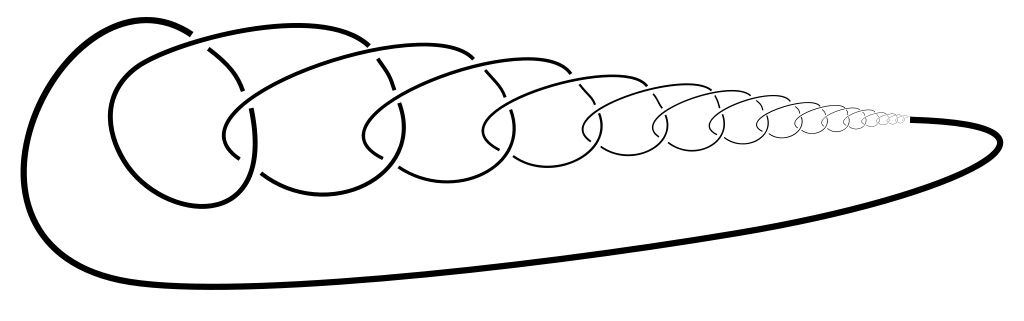
\includegraphics[width=0.5\linewidth]{wild_knot.png}
    \caption{Węzeł dziki}
\end{figure}

Zastanówmy się, jakim formalizmem opisać manipulowanie fizycznym sznurkiem, by wykluczyć węzły dzikie z~naszych rozważań.
Nie można użyć izotopii (dwa węzły są izotopijne, jeśli istnieje ciągła funkcja $F \colon S^1 \times [0, 1] \to \R^3$ taka, że $F(-, 0)$ jest pierwszym, zaś $F(-,1)$ drugim węzłem), gdyż każdy węzeł jest izotopijny z punktem:

{\color{red}\textbf{Tu brakuje obrazka.}}

W podobny sposób moglibyśmy przekształcić dowolny węzeł w~niewęzeł.
Teoria, w~której wszystkie obiekty są takie same, nie jest zbyt ciekawa.
Zwykła izotopia nie oddaje dobrze tego, czym jest równoważność węzłów wykonanych z~prawdziwego sznurka.
Trzeba od niej wymagać dodatkowo, by była gładka albo lokalnie płaska.
Z twierdzenia o rozszerzaniu izotopii wynika, że można ją wtedy podnieść do izotopii otaczającej.
Ta ostatnia uwzględnia, jak węzeł leży w~przestrzeni i okazuje się być właściwym pojęciem równości dla teorii węzłów:

\begin{definition}[izotopia otaczająca] \label{def_ambient_isotopy}
    Niech $N, M$ będą rozmaitościami, zaś $K_1, K_2 \colon N \to M$ włożeniami.
    Ciągłe odwzorowanie $F \colon M \times [0,1] \to M$ spełniające następujące warunki:
    \begin{enumerate}
        \item funkcja $F(-, 0)$ jest odwzorowaniem tożsamościowym,
        \item każda z funkcji $F(-, t)$ jest homeomorfizmem,
        \item złożenie $F(-, 1)$ z pierwszym włożeniem $K_1$ daje drugie włożenie $K_2$
    \end{enumerate}
    nazywamy izotopią otaczającą przenoszącą $K_1$ na $K_2$.
\end{definition}

W topologii rozważa się włożenia dowolnych rozmaitości, nam wystarczy jeden szczególny przypadek $N = S^1$ oraz $M = \R^3$.
Intuicyjnie, funkcja $F$ zniekształca przestrzeń $\R^3$ tak, że w~chwili początkowej $t = 0$ widzimy pierwszy, zaś w~chwili końcowej $t = 1$ drugi węzeł.
Izotopia otaczająca nie pozwala na ściąganie zaplątanych fragmentów do punktu.

{\color{red}\textbf{Homeomorfizmy $F_t$ można zastąpić przez dyfeomorfizmy zachowujące orientację. ???}}

\begin{definition}[węzeł]
    \label{def:knot}
    \index{węzeł}
    Gładkie włożenie $S^1 \to \R^3$ otaczająco izotopijne z~zamkniętą łamaną bez samoprzecięć nazywamy węzłem poskromionym.
\end{definition}

Przez prawie całą książkę interesować nas będą jedynie węzły poskromione,
dlatego jeśli nie zaznaczono inaczej, przez węzeł rozumiemy węzeł poskromiony.
Istnieje jeszcze jedna, konkurencyjna definicja węzłów równoważnych:

\begin{proposition}
    \label{equivalent_knots_2}
    Dwa węzły są równoważne, gdy jeden z~nich jest obrazem drugiego przez zachowujący orientację homeomorfizm $\R^3 \to \R^3$.
\end{proposition}

Stwierdzenie to przestaje być prawdziwe po zastąpieniu przestrzeni $\R^m$ przez $S^m$.

\begin{proof}
    Podany niżej dowód pochodzi z~książki ,,Topology from the differentiable viewpoint'' Johna Milnora.
    Musimy pokazać, że dyfeomorfizm $f \colon \R^m \to \R^m$ jest gładko izotopijny z~identycznością.
    Translacje są izotopiami, więc bez straty ogólności zakładamy, że $f(0) = 0$.
    Pochodna $f$ w~zerze jest dana wzorem $\mathrm{d}f_0(x) = \lim_{t \to 0} f(tx) /t$,
    naturalną definicję izotopii $F \colon \R^m \times [0, 1] \to \R^m$ stanowi więc
    \[
        F(x, t) = \begin{cases}
            \mathrm{d}f_0(x) & t = 0 \\
            f(tx) / t & 0 < t \le 1
        \end{cases} .
    \]

    Funkcja $F$ jest gładka, gdyż na mocy lematu Hadamarda funkcja $f$ zapisuje się jako suma $x_1 g_1(x) + \ldots + x_mg_m(x)$,gdzie funkcje $g_i$ są gładkie, co jakoś kończy dowód.
\end{proof}

Formalnie węzły to pewne odwzorowania, więc prawidłowym sposobem na zapisanie, że są izotopijne (czyli dla nas: równe), jest $K_1 \simeq K_2$.
Ponieważ nie prowadzi to do problemów, będziemy jednak stosować zapis $K_1 = K_2$.
Jednocześnie często węzeł (jako odwzorowanie) nie będzie odróżniany od obrazu tego odwzorowania.

\begin{definition}[splot, ogniwo]
    \label{def_link}
    \index{splot}
    Sumę parami rozłącznych węzłów $K_1, K_2, \ldots, K_n$ nazywamy splotem.
    Składniki sumy nazywamy ogniwami.
\end{definition}

Przez analogię do węzłów mówimy, że dwa sploty są takie same, jeśli jeden jest obrazem drugiego przez zachowujący orientację homeomorfizm $\R^3 \to \R^3$.
W~takiej sytuacji obydwa sploty mają tyle samo ogniw.

\begin{example}
    \index{splot!Hopfa}
    Splot Hopfa to najprostszy splot nietrywialny, którym w~1931 r. zajmował się Heinz Hopf, topolog niemiecki, w~ramach badań nad tzw. rozwłóknieniem (Hopf fibration).
    Whitehead w~1934 odkrył kontrprzykład do nieudanego dowodu hipotezy Poincarego.
    Był nim splot o~dwóch składowych przedstawiony na poniższym rysunku.

    \begin{figure}[H]
        \begin{minipage}[b]{.48\linewidth}
            \centering
            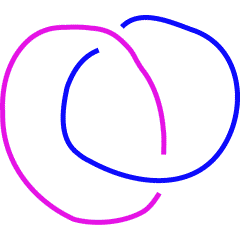
\includegraphics[width=0.5\linewidth]{../data/mixed/L2a1.png}
            \subcaption{splot Hopfa}
        \end{minipage}
        \begin{minipage}[b]{.48\linewidth}
            \centering
            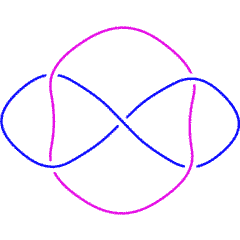
\includegraphics[width=0.5\linewidth]{../data/mixed/L5a1.png}
            \subcaption{splot Whiteheada}
        \end{minipage}
    \end{figure}
\end{example}

Jeśli dwa węzły są równoważne, to ich dopełnienia są oczywiście homeomorficzne.
Pytanie o~prawdziwość implikacji odwrotnej jako pierwszy zadał najprawdopodobniej w~1908 roku Tietze (,,Über die topologischen Invarianten mehrdimensionaler Mannigfaltigkeiten'').
W roku 1987 pokazano, że istnieją co najwyżej dwa węzły o~zadanym dopełnieniu (\cite{culler87}).
Dwa lata później poznaliśmy pozytywną odpowiedź na pytanie Tietzego: każdy węzeł jest wyznaczony jednoznacznie przez swoje dopełnienie.

\begin{theorem}[Gordon, Luecke, 1989]
    \label{thm_gordon_luecke}
    \index{twierdzenie!Gordona-Lueckego}
    Poskromione węzły o~homeomorficznych (z zachowaniem orientacji) dopełnieniach są wzajemnie izotopijne.
\end{theorem}

\begin{proof}[Niedowód]
    Wynika to z~ogólniejszego stwierdzenia:
    nietrywialna chirurgia Dehna na węźle w~3-sferze nigdy nie daje 3-sfery.
    Pełny dowód zawiera praca \cite{gordon89}.
\end{proof}

Twierdzenie to zamienia problem lokalny (czy dwa węzły w kuli $S^3$ są równoważne?) w~problem globalny (czy dwie przestrzenie topologiczne są homeomorficzne?).
Whitehead w~pracy \cite{whitehead37} z~1937 roku podał nieskończenie wiele splotów, których dopełnienia wyglądają jak dopełnienia splotu Whiteheada.
Odpowiednik twierdzenia \ref{thm_gordon_luecke} dla splotów jest więc fałszywy.

Poniższa definicja nie jest nam jeszcze potrzebna, ale wygodnie przytoczyć ją już teraz.

\begin{definition}[rozszczepialność]
    \index{splot!rozszczepialny}
    Jeżeli splot $L$ można zanurzyć w przestrzeni $\R^3$ tak, że niektóre jego ogniwa będą leżeć nad pewną rozłączną ze splotem płaszczyzną, zaś pozostałe pod nią, to powiemy, że splot $L$ jest rozszczepialny.
\end{definition}

Liczbę nierozszczepialnych splotów, pierwszych lub złożonych, zebrano w tabeli.
Źródło: baza danych OEIS, ciąg \href{https://oeis.org/A086825}{A086825}.

\renewcommand*{\arraystretch}{1.4}
\footnotesize
\begin{longtable}{lccccccccc}
    \hline
    \textbf{skrzyżowania}  &  0  &  1  &  2  &  3  &  4  &  5  &  6   &  7   &  8   \\  \hline  \endhead
    sploty                 &  1  &  0  &  1  &  1  &  3  &  4  &  15  &  24  &  82  \\
    \hline
\end{longtable}
\normalsize

\section{Diagramy. Ruchy Reidemeistera}
Chociaż w~świetle definicji \ref{def:knot} węzły są pewnymi regularnymi podzbiorami przestrzeni $\R^3$,
z kombinatorycznego punktu widzenia wygodniej jest rysować je na płaszczyźnie.

\begin{definition}[orientacja]
    \index{węzeł!zorientowany}
    Węzeł, w~którym wybrano kierunek, w~którym należy się po nim poruszać, nazywamy zorientowanym.
\end{definition}

\begin{definition} [diagram] \label{def_diagrams}
    \index{diagram}
    Cień to rzut węzła $K \subseteq \R^3$ na płaszczyznę.
    Cień razem z~informacją o~tym, jak przebiegają skrzyżowania i pozbawiony katastrof: potrójnych przecięć, stycznych czy dziobów nazywamy diagramem.
\end{definition}

{\color{red}\textbf{Narysować katastrofy}}

\begin{definition} [włókno]
    \index{włókno}
    Fragment diagramu, który biegnie między dwoma kolejnymi tunelami, czyli podskrzyżowaniami, nazywamy włóknem.
\end{definition}

\begin{definition} [nić]
    \index{nić}
    Fragment diagramu, który biegnie między dwoma kolejnymi skrzyżowaniami nazywamy nicią.
\end{definition}

Nici powstają z włókien przez rozcięcie ich przy każdym nadskrzyżowaniu.

\begin{proposition}
    Niech $K$ będzie węzłem.
    Zbiór diagramów jest otwarty i~gęsty w~zbiorze wszystkich rzutów.
\end{proposition}

\begin{proof}
    Rzut splotu na równoległe płaszczyzny jest taki sam, a te można sparametryzować prostymi przechodzącymi przez początek układu współrzędnych, które tworzą przestrzeń rzutową $\R \mathbb P^2$.
    Niech $S$ będzie zbiorem prostych, które dają złe rzuty.
    Wystarczy pokazać jego nigdziegęstość.
    Okazuje się, że $S$ jest też jednowymiarowy.
    (Dowód za \cite{crowell63}).
\end{proof}

Wynika stąd, że każdy węzeł ma wiele diagramów.
Mając dane dwa różne diagramy chcielibyśmy wiedzieć, czy reprezentują ten sam węzeł.
Na szczęście Reidemeister w latach 20. XX wieku podał proste kryterium rozstrzygające ten problem.
Najpierw zdefiniujmy trzy lokalne operacje na diagramach.

\begin{definition}
    \index{ruchy Reidemeistera}
    Trzy ruchy Reidemeistera, $R_1$, $R_2$, oraz $R_3$, to następujące deformacje diagramu:
    \[
        \underbrace{\begin{tikzpicture}[baseline=-0.65ex,scale=0.1]
        \begin{knot}[clip width=5]
            \strand[thick] (-5, 10) to [in=left, out=down] (2, -5);
            \strand[thick] (5, 0) to [in=right, out=down] (2, -5);
            \strand[thick] (5, 0) to [in=right, out=up] (2, 5);
            \strand[thick] (-5, -10) to [in=left, out=up] (2, 5);
        \end{knot}
        \end{tikzpicture}
        \, \cong \,
        \begin{tikzpicture}[baseline=-0.65ex,scale=0.1]
        \begin{knot}[clip width=5]
            \strand[thick] (0,10) to (0,-10);
        \end{knot}
        \end{tikzpicture}}_{R_1}
        %%%
        \quad \quad \quad
        \underbrace{\begin{tikzpicture}[baseline=-0.65ex,scale=0.1]
        \begin{knot}[clip width=5]
            \strand[thick] (-5, 10) to [in=up, out=down] (5, 0);
            \strand[thick] (-5, -10) to [in=down, out=up] (5, 0);
            \strand[thick] (5, 10) to [in=up, out=down] (-5, 0);
            \strand[thick] (5, -10) to [in=down, out=up] (-5, 0);
        \end{knot}
        \end{tikzpicture}
        \, \cong \,
        \begin{tikzpicture}[baseline=-0.65ex,scale=0.1]
        \begin{knot}[clip width=5]
            \strand[thick] (-5, 10) to [in=up, out=down] (-2, 0);
            \strand[thick] (-5, -10) to [in=down, out=up] (-2, 0);
            \strand[thick] (5, 10) to [in=up, out=down] (2, 0);
            \strand[thick] (5, -10) to [in=down, out=up] (2, 0);
        \end{knot}
        \end{tikzpicture}}_{R_2}
        %%%
        \quad \quad \quad
        \underbrace{\begin{tikzpicture}[baseline=-0.65ex,scale=0.1]
        \begin{knot}[clip width=5, flip crossing/.list={1,2,3}]
            \strand[thick] (-10, -10) -- (10, 10);
            \strand[thick] (-10, 10) -- (10, -10);
            \strand[thick] (-10, 0) to [in=left, out=right] (0, 10);
            \strand[thick] (10, 0) to [in=right, out=left] (0, 10);
        \end{knot}
        \end{tikzpicture}
        \, \cong \,
        \begin{tikzpicture}[baseline=-0.65ex,scale=0.1]
        \begin{knot}[clip width=5, flip crossing/.list={1,2,3}]
            \strand[thick] (-10, -10) -- (10, 10);
            \strand[thick] (-10, 10) -- (10, -10);
            \strand[thick] (-10, 0) to [in=left, out=right] (0, -10);
            \strand[thick] (10, 0) to [in=right, out=left] (0, -10);
        \end{knot}
        \end{tikzpicture}}_{R_3}
    \]
\end{definition}

Ruch $R_i$ operuje więc na $i$ łukach diagramu.
Reidemeister w~swojej pierwszej pracy przyjął inną kolejność,
jego drugi ruch jest naszym pierwszym.

\begin{theorem}[Reidemeister, 1927]
    \label{thm:reidemeister}
    Każdy splot posiada diagram.
    Dwa diagramy przedstawiają równoważne sploty,
    wtedy i~tylko wtedy gdy pierwszy można otrzymać z~drugiego
    wykonując skończenie wiele ruchów Reidemeistera
    oraz gładko deformując łuki bez zmiany biegu skrzyżowań.
\end{theorem}

Twierdzenie Reidemeistera jest prawdziwe zarówno dla splotów zorientowanych jak i~takich, które nie posiadają orientacji.

\begin{proof}
    Szkielet dowodu można znaleźć w~książce Burdego i~Zieschanga.
    Kluczowe pomysły zawiera ,,Knots, links, braids and $3$-manifolds''
    Prasołowa i~Sosińskiego.
    Innym przystępnym źródłem jest podręcznik \cite{murasugi96} Murasugiego ,,Knot theory and its applications''.
\end{proof}

{\color{red}\textbf{Brakuje prawdziwych cytowań}}

W praktyce twierdzenia \ref{thm:reidemeister} nie stosuje się bezpośrednio do diagramów splotów.
Jednym z~powodów jest wynik Cowarda i~Lackenby'a (\cite{coward11}): jeśli na dwóch diagramach tego samego węzła widać łącznie $n$ skrzyżowań, to ,,wystarcza''
\[
    R(n) = 2^{2^{\ldots^{2^n}}}
\]
ruchów Reidemeistera, by przejść między nimi; piętrowa potęga ma $10^{1000000n}$ warstw.
Gdy jeden z~diagramów jest pozbawiony skrzyżowań, czyli przedstawia niewęzeł, wystarcza $(236n)^{11}$ ruchów.
Zapewne lepsze ograniczenia istnieją, ale ich nie znamy.
Ważne jest to, że wielkość $R(n)$ jest skończona.

{\color{red}\textbf{Przedstawić rozumowanie (piramidka z węzłami), dlaczego to nie jest takie oczywiste.}}

Zamiast tego definiuje się niezmienniki, czyli funkcje ze zbioru wszystkich diagramów, które nie zmieniają swojej wartości podczas wykonywania ruchów Reidemeistera.
Kiedy pewien niezmiennik przyjmuje różne wartości na dwóch diagramach, te przedstawiają dwa istotnie różne sploty.
Gdy wartości są te same, nie dostajemy żadnej informacji.
Sploty mogą być równoważne albo nie.
Niezmienniki będą nam stale towarzyszyć w~wędrówce po krainie węzłów.

% koniec sekcji Ruchy Reidemeistera

%Niestety pomimo upływu czasus, nikt nie napisał komputerowego programu realizującego ten algorytm (stan na 1994).
%Może podejmie się tego Czytelnik?
%Inne algorytmy istnieją, jednak wszystkie działają w~wykładniczym czasie.

W 1961 roku W. Haken \cite{haken61} podał niezawodny przepis na wykrycie diagramu niewęzła,
częściowo rozwiązując jeden z~ważniejszych problemów teorii węzłów.
Przez wiele lat nikt nie podjął się implementacji tego algorytmu,
udało się to niedawno Burtonowi, Budneyowi oraz Petterssonowi w~komputerowym programie Regina\footnote{Dostępny pod adresem \url{https://regina-normal.github.io/}.} na przełomie tysiącleci.
Burton, Rubinstein i~Tillman pokazali w~pracy \cite{burton12}, jak sprawdzać,
czy powierzchnia normalna na striangulowanej 3-rozmaitości jest (nie)ściśliwa w~czasie wykładniczym.
To okazało się być wystarczającym do udzielenia negatywnej odpowiedzi na pytanie Thurstona:
,,czy przestrzeń Seiferta-Webera jest rozmaitością Hakena?'',
a zatem wykraczającego poza poziom tej pracy.
Patrz także {\url{http://geometrygames.org/SnapPea/index.html}.

{\color{red}\textbf{Dowiązać tutaj wszystkie wykrywacze niewęzła opisane w książce}}

Przykładami trudnych w~rozpoznaniu niewęzłów są: niewęzeł Goritza, Freedmana.
Więcej trudnych niewęzłów zawiera praca \cite{zanellati16} autorstwa C. Petronio oraz A. Zanellatiego.

\begin{figure}[H]
    \begin{minipage}[b]{.32\linewidth}
        \centering
        
\includegraphics[width=\linewidth]{../data/missing.jpg}
        \subcaption{normalny}
    \end{minipage}
    \begin{minipage}[b]{.32\linewidth}
        \centering
        
\includegraphics[width=\linewidth]{../data/missing.jpg}
        \subcaption{Goritza}
    \end{minipage}
    \begin{minipage}[b]{.32\linewidth}
        \centering
        
\includegraphics[width=\linewidth]{../data/missing.jpg}
        \subcaption{Freedmana}
    \end{minipage}
\end{figure}

Zanim opowiemy, jak dotąd przebiegała klasyfikacja węzłów o małej liczbie skrzyżowań, zdefiniujemy klasę splotów ze specjalnymi diagramami.

\begin{definition}[alternacja]
    \index{węzeł!alternujący}
    Diagram splotu, gdzie podczas poruszania się wzdłuż każdego ogniwa nad- oraz podskrzyżowania mijane są naprzemiennie, nazywamy alternującym.
    Splot jest alternujący, jeśli posiada alternujący diagram.
\end{definition}

Około 1961 roku Fox zapytał ,,What is an alternating knot?''.
Szukano takiej definicji węzła alternującego, która nie odnosi się bezpośrednio do diagramów, aż w~2015 roku Joshua Greene podał geometryczną charakteryzację: nierozdzielczy splot w $S^3$ jest alternujący wtedy i tylko wtedy, gdy ogranicza dodatnią oraz ujemną określoną powierzchnię rozpinającą \cite{greene17}.
% definite spanning surface

Sundberg oraz Thistlethwaite pokazali w 1998 roku, że liczba splotów alternujących rośnie wykładniczo (\cite{sundberg98}):

\begin{proposition}
    Niech $a_n$ oznacza liczbę pierwszych, alternujących supłów o~$n$ skrzyżowaniach.
    Wtedy
    \begin{equation}
        a_n \sim (3c_1/4\sqrt{\pi})n^{-5/2}\lambda^{n-3/2},
    \end{equation}
    gdzie zarówno $c_1$, pierwszy współczynnik rozwinięcia Taylora funkcji $\Phi(\eta)$ zdefiniowanej w \cite{sundberg98}, jak i $\lambda$ są jawnie znanymi stałymi:
    \begin{align}
        c_1 & = \sqrt{\frac{5^7 \cdot (21001 + 371 \sqrt{21001})^3}{2 \cdot 3^{10} \cdot (17 + 3\sqrt{21001})^5}} \\
        \lambda & = \frac {1}{40} (101 + \sqrt{21001})
    \end{align}
    Niech $A_n$ oznacza liczbę pierwszych, alternujących splotów o $n$ skrzyżowaniach.
    Wtedy $A_n \approx \lambda^n$, dokładniej: jeśli $n \ge 3$, to
    \begin{equation}
        \frac{a_{n-1}}{16n - 24} \le A \le \frac{a_n - 1}{2}.
    \end{equation}
\end{proposition}

Czasami będziemy używać słów przed ich zdefiniowaniem, tak jak uczyniliśmy tutaj: węzły pierwsze i~supły pojawiają się odpowiednio w definicjach \ref{primeknot}, \ref{def:tangle}.
Książkę trzeba więc przeczytać co~najmniej dwa razy.

\begin{proposition}
    Niech $a_n$ oznacza liczbę pierwszych, alternujących supłów o~$n$ skrzyżowaniach.
    Wtedy funkcja tworząca $f(z) = \sum_n a_n z^n$ spełnia równanie
    \begin{equation}
    f(1+z) - f(z)^2 - (1+f(z))q(f(z)) -z - \frac{2z^2}{1-z} = 0,
    \end{equation}
    gdzie $q(z)$ jest pomocniczą funkcją
    \begin{equation}
        q(z) = \frac{2z^2 - 10z - 1 + \sqrt{(1-4z)^3}} {2(z+2)^3} - \frac{2}{1+z} -z + 2.
    \end{equation}
\end{proposition}

Fakt ten stanowi raczej ciekawostkę i także pochodzi z cytowanej wcześniej pracy \cite{sundberg98}.

\subsection{Historia tablic węzłów}
Pierwszą osobą, która podjęła się szukania węzłów, był Peter Guthrie Tait, szkocki fizyk.
Razem z Thomsonem (lordem Kelvinem) wierzyli, że węzły są kluczem do zrozumienia widma spektroskopowego różnych pierwiastków: na przykład atom sodu mógł być splotem Hopfa ze względu na dwie linie emisyjne.
Eksperyment Michelsona-Morleya z 1887 roku zabił ich ,,wirową teorię atomu'', ale nie miało to znaczenia dla teorii węzłów jako działu matematyki.

Używana po dziś dzień strategia, którą przyjął Tait, jest stosunkowa prosta: narysować wszysktie możliwe diagramy o~zadanym indeksie skrzyżowaniowym, po czym połączyć ze sobą te, które przedstawiają jeden węzeł.
Na potrzeby pierwszego etapu Tait wymyślił schemat kodowania diagramów.
Wiele lat wcześniej, Gauss wraz ze swoim uczniem Listingiem badał węzły i~opracował (niezależnie!) podobną notację.
My przytoczymy opis dalszego ulepszenia tej metody, zwanego notacją Dowkera-Thistletwaite’a.

Tait wykorzystując swoją notację podał w~1876 pierwszą tablicę piętnastu węzłów o~mniej niż ośmiu skrzyżowaniach.
Nie należy traktować tego jako skromny wynik: nie miał on do dyspozycji żadnych twierdzeń topologicznych do odróżniania węzłów.
Onieśmielony przez liczbę możliwych ciągów dla kolejnych indeksów skrzyżowaniowych, powstrzymał się przed rozszerzaniem swojej tablicy.
To właśnie grupowanie diagramów przedstawiających ten sam węzeł, a~nie samo szukanie wszystkich możliwych diagramów, sprawia trudność.

Aby sobie pomóc, Tait znalazł lokalną modyfikację diagramu, która nie zmienia indeksu skrzyżowaniowego, znaną obecnie jako flype.

\[
\begin{tikzpicture}[baseline=-0.65ex, scale=0.1]
\begin{knot}[clip width=5, end tolerance=1pt, flip crossing/.list={1}]
    \strand[semithick] (-21, -5) [in=180, out=0] to (-7, 5);
    \strand[semithick] (-21, 5) [in=180, out=0] to (-7, -5);
    \draw (-7, -7) rectangle (7, 7);
    \node at (0, 0) {\Huge {$T$}};
    \draw[semithick] (7, -5) to (21, -5);
    \draw[semithick] (7, 5) to (21, 5);
\end{knot}
\end{tikzpicture}
\quad \cong_{\mathrm{flype}} \quad
\begin{tikzpicture}[baseline=-0.65ex, scale=0.1]
\begin{knot}[clip width=5, end tolerance=1pt]
    \strand[semithick] (21, -5) [in=0, out=180] to (7, 5);
    \strand[semithick] (21, 5) [in=0, out=180] to (7, -5);
    \draw (-7, -7) rectangle (7, 7);
    \node at (0, 0) {\rotatebox[origin=c]{-180}{\Huge $T$}};
    \draw[semithick] (-7, -5) to (-21, -5);
    \draw[semithick] (-7, 5) to (-21, 5);
\end{knot}
\end{tikzpicture}
\]

Inną taktykę szukania węzłów przyjał wielebny Thomas Kirkman: zaczynał od małego zbioru "nieredukowalnych" rzutów, do których systematycznie dokładał skrzyżowania.
Tait przeczytał pracę Kirkmana, po czym w~latach 1884/1885 opracował listę węzłów alternujących o~mniej niż 11 skrzyżowaniach.
Tuż przed oddaniem jej do druku odkrył inny spis węzłów stworzony przez amerykańskiego naukowca Charlesa Little'a.
Znalazł wtedy jeden duplikat u~siebie, natomiast u Little'a jeden duplikat i~jedno pominięcie.

Zachęcony przez Taita, Little zabrał się za alternujące węzły o~11 skrzyżowaniach i~za trudniejsze zadanie, stablicowanie węzłów niealternujących, czyli takich, które nie posiadają alternującego diagramu.
Jak wynika z~pierwszej pracy Taita, początkowo nie wierzono, że takie w~ogóle istnieją.
Dowód znaleziono wiele lat później, niealternujące są $8_{19}$, $8_{20}$, $8_{21}$, ale nie pierwsze węzły o mniejszej liczbie skrzyżowań.
Patrz twierdzenie \ref{prp:bankwitz}.
Little pracował przez sześć lat (1893 -- 1899) i~znalazł 43 niealternujące węzły o~10 skrzyżowaniach.
Żadnego nie pominął, ale trafił mu się jeden duplikat.

W kolejnych dziesięcioleciach nie nastąpił znaczący postęp, zarówno w~rozszerzaniu tablic jak i~sprawdzaniu tych już istniejących.
Haseman w~1918 roku znalazł achiralne węzły o~12 i~14 skrzyżowaniach.
W 1927 roku Alexander z~Briggsem przy użyciu pierwszej grupy homologii rozgałęzionego nakrycia cyklicznego (!) potrafili odróżnić od siebie dowolne dwa węzły (z~pominięciem trzech par) o~co najwyżej 9 skrzyżowaniach.
Reidemeister poradził sobie z~tymi wyjątkami w~1932 roku, korzystając z~indeksu zaczepienia i~homomorfizmów z~grupy węzła na grupy diedralne.
% branch curves in irregular covers associated to homomorphisms of the knot group onto dihedral groups

%%%%% Tait, Little wyprodukowali prawie bezbłędną tablicę węzłów o~co najwyżej 11 skrzyżowaniach przy użyciu grafów.

Dopiero Conway w~latach sześćdziesiątych minionego wieku znalazł pierwsze węzły o~mniej niż 12 skrzyżowaniach oraz wszystkie sploty o~mniej niż 11 skrzyżowaniach w~oparciu o~pomysły Kirkmana.
% An enumeration of knots and links, 1970.
Zajęło mu to jedynie kilka godzin!
Conway znalazł 1 duplikat oraz 11 pominięć w~tablicach Little'a, ale sam popełnił 4 pominięcia.
Przeoczył między innymi słynny duplikat w~niealternującej tablicy Little'a, parę Perko.
% 1974?
Przyczyną było prawdopodobnie to, że dwa diagramy miały różny spin:
Little błędnie twierdził, że spin minimalnego diagramu jest niezmiennikiem, gdyż błędnie założył, że flype oraz 2-przejścia wystarczają do zmiany jednego minimalnego diagramu w~inny.

Pominęcia w~tablicy Conwaya znalazł Caudron w~1980 roku.
Nieopublikowany manuskrypt Bonahona, Siebenmanna klasyfikuje węzły algebraiczne.
Z~nielicznymi niealgebraicznymi węzłami do 11 skrzyżowań poradził sobie Perko około 1980 roku (,,Invariants of 11-crossing knots'').
To był kres ery ręcznych obliczeń.

Na początku lat osiemdziesiątych Dowker i~Thistlethwaite stabularyzowali z~pomocą komputera węzły do 13 skrzyżowań.
Przez blisko dekadę nic się nie działo, aż grupa studentów wygrała dostęp do superkomputera Cray.
Razem z~Hoste znaleźli alternujące węzły do 14 skrzyżowań, jednocześnie sprawdzając istniejące tabele Thistlethwaite'a.
Około roku 1998 Hoste z~Weeksem (oraz niezależnie Thistlethwaite) znaleźli 1701936 pierwszych węzłów do 16 skrzyżowań.
Spośród nich, tylko 32 nie jest węzłami hiperbolicznymi, wszystkie pozostałe poddają się maszynerii geometrii hiperbolicznej.

\subsection{Hipotezy Taita}
\begin{conjecture}[I hipoteza Taita]
    \label{conj_tait_i}
    \index{hipoteza!Taita}
    Zredukowany alternujący diagram splotu ma minimalny indeks skrzyżowaniowy.
\end{conjecture}
% To bardzo ważny rezultat, którego prawdziwość przypuszczał już P. G. Tait w~XIX wieku.
% Nikt nie był w~stanie podać dowodu przed pojawieniem się wielomianu Jonesa.

Najpierw znaleziono dowód korzystający z wielomianu Jonesa (Kauffman \cite{kauffman87}, Murasugi \cite{murasugi87}, Thistlethwaite \cite{thistlethwaite87}, wszystkie prace z 1987 roku).
Trzydzieści lat później Greene zaprezentował geometryczne podejście do problemu w \cite{greene17}.

\begin{conjecture}[II hipoteza Taita]
    \label{conj_tait_ii}
    Achiralny splot alternujący ma zerowy spin.
\end{conjecture}

Pierwsze dowody pochodzą znowu od Kauffmana \cite{kauffman87} oraz Thistlethwaite'a \cite{thistlethwaite87}.

\begin{conjecture}[III hipoteza Taita]
    \label{conj_tait_iii}
    Niech $D_1, D_2$ będą zredukowanymi alternującymi diagramami zorientowanego pierwszego splotu.
    Wtedy diagram $D_2$ można otrzymać z~$D_1$ korzystając jedynie z~ruchu \emph{flype}.
\end{conjecture}

Tę hipotezę udowodnił Menasco z Thistlethwaitem, \cite{menasco91}.
Wynika z~niej, że dwa zredukowane diagramy alternujące tego samego węzła mają ten sam spin: ruch flype nie zmienia spinu (dla niektórych to jest II hipoteza).	
My pokażemy nieco później, czyli po poznaniu wielomianu Jonesa, że wszystkie trzy hipotezy są prawdziwe.

\textbf{Wstawić odniesienia do naszego dowodu}

\subsection{Metody kodowania}
\subsubsection{Notacja Alexandera-Briggsa}
Najbardziej tradycyjny, wprowadzony w~1927 roku sposób opisu węzłów do 9 skrzyżowań.
Węzły kodowane są przez indeks skrzyżowaniowy z dolnym indeksem informującym o miejscu w tablicy węzłów.
Porzadek jest umowny i nie ma żadnego głębszego znaczenia, jego wybór należy do osoby, która jako pierwsza znajdzie wszystkie węzły o danej liczbie skrzyżowań.
Jedyną regularnością jest to, że węzeł skręcony występuje zawsze po węźle torusowym.

Rolfsen w 1976 stworzył z kilkoma błędami tablicę diagramów pierwszych węzłów do 10 skrzyżowań.
Para Perko $10_{161}, 10_{162}$ przedstawia ten sam węzeł, zaś górne skrzyżowanie w~$10_{144}$ powinno być zmienione.
Ostatnie cztery węzły dostały nowe numery, by uniknąć duplikatu.
Kolejną usterką tablicy jest to, że notacja Conwaya oraz wielomian Alexandera dla węzłów $10_{83}$ oraz $10_{86}$ są zamienione miejscami.
Tu czyha pułapka: Stojmenow, nowe wydanie książki Rolfsena, atlas węzłów Bar-Natana oraz tablica niezmienników węzłowych Livingstona naprawiają to przez wymianę podpisów.
Podręcznik Kawauchiego wymienia diagramy.
% http://stoimenov.net/stoimeno/homepage/ptab/

\subsubsection{Notacja Dowkera-Thistlethwaite'a}
Poprawia notację Taita.
Należy ustalić minimalny diagram węzła, dowolny punkt początkowy oraz kierunek i zacząć przemierzać węzeł.
Za każdym razem, kiedy mijamy skrzyżowanie, przypisujemy mu kolejną liczbę naturalną, zaczynając od jedynki.
Jeżeli znajdujemy się nad skrzyżowaniem, parzyste etykiety zapisujemy z przeciwnym znakiem.
Kiedy skończymy, każde skrzyżowanie będzie mieć dwie etykiety.

\begin{definition}
	Ciąg parzystych liczb występujących na diagramie kolejno przy $1, 3, \ldots$ nazywamy kodem Dowkera-Thistlethwaite'a.
\end{definition}

Opisany powyżej kod nie jest idealny, ponieważ odtworzony z niego węzeł może być lustrzanym odbiciem wyjściowego.
Ogólniej, odbicie dowolnego składnika sumy spójnej nie zmienia kodu całego węzła.
Nie stanowi to jednak dużego problemu, ponieważ notacja została stworzona na potrzeby tablicowania węzłów pierwszych, a~te są niezorientowane.

Zaczynając od zredukowanego diagramu o $n$ skrzyżowaniach nie można doprowadzić do sytuacji, gdzie do pewnego skrzyżowania przypisane są dwie kolejne liczby całkowite.
Dzięki temu problem można przetłumaczyć na język teorii grafów.
Rozpatrzmy graf $G$, którego wierzchołkami są liczby $1, 2, \ldots, 2n$.
Połączmy niesąsiadujące modulo $2n$ wierzchołki o różnej parzystości krawędziami.
Graf ten powstaje przez usunięcie cyklu Hamiltona (łączącego kolejne liczby) z pełnego grafu dwudzielnego.
Zbiór par etykiet przy skrzyżowaniach węzła to skojarzenie doskonałe w grafie $G$.
Liczba skojarzeń prawie pokrywa się z rozwiązaniem zadania znanego w literaturze jako ,,problème des ménages'': na ile sposobów $n$ małżeństw można posadzić przy okrągłym stole tak, by żadne małżeństwo nie siedziało obok siebie i~każdy mężczyzna znalazł się obok dwóch kobiet?
Ustawienia, które powstają przez cykliczne permutowanie należy uznać za tożsame.
Gilbert znalazł w \cite{gilbert56} wzór na $a_n$, liczbę różnych kodów:
\begin{align}
u(m, t) & = 2m \sum_{k=0}^m {2m-k \choose k} \cdot (m-k)! \cdot \frac{(t-1)^k}{2m - k}  \\
a(n) & = \frac{1}{n} \sum_{d\mid n} \left(\frac{n}{d}\right)^d \cdot u \left(d, 1 - \frac{d}{n}\right) \cdot \varphi \left(\frac{n}{d}\right)
\end{align}

Kilka początkowych wartości to $a_3 = 1, 2, 5, 20, 87, 616, 4843, 44128, 444621, \ldots$ (ciąg A002484 w OEIS).

\subsubsection{Notacja Conwaya}
Wprowadzona przez Conwaya w~pracy \cite{conway70}.
Opiera się na pojęciu supła, dlatego więcej szczegółów przedstawiamy dopiero w definicji \ref{conway_notation}.

\section{Ruchy Reidemeistera}
\label{sec:reidemeister_moves}
W kombinatorycznej teorii węzłów diagramy są dużo ważniejsze od gładkich włożeń okręgu w~przestrzeń $\R^3$,
dlatego przytoczymy proste kryterium decydujące o~tym,
kiedy dwa diagramy przedstawiają jeden węzeł.
Najpierw zdefiniujmy trzy lokalne operacje na diagramach.

\begin{definition}
    \index{ruchy Reidemeistera}
    Trzy ruchy Reidemeistera, $R_1$, $R_2$, oraz $R_3$, to następujące deformacje diagramu:
    \[
        \underbrace{\begin{tikzpicture}[baseline=-0.65ex,scale=0.1]
        \begin{knot}[clip width=5]
            \strand[thick] (-5, 10) to [in=left, out=down] (2, -5);
            \strand[thick] (5, 0) to [in=right, out=down] (2, -5);
            \strand[thick] (5, 0) to [in=right, out=up] (2, 5);
            \strand[thick] (-5, -10) to [in=left, out=up] (2, 5);
        \end{knot}
        \end{tikzpicture}
        \, \cong \,
        \begin{tikzpicture}[baseline=-0.65ex,scale=0.1]
        \begin{knot}[clip width=5]
            \strand[thick] (0,10) to (0,-10);
        \end{knot}
        \end{tikzpicture}}_{R_1}
        %%%
        \quad \quad \quad
        \underbrace{\begin{tikzpicture}[baseline=-0.65ex,scale=0.1]
        \begin{knot}[clip width=5]
            \strand[thick] (-5, 10) to [in=up, out=down] (5, 0);
            \strand[thick] (-5, -10) to [in=down, out=up] (5, 0);
            \strand[thick] (5, 10) to [in=up, out=down] (-5, 0);
            \strand[thick] (5, -10) to [in=down, out=up] (-5, 0);
        \end{knot}
        \end{tikzpicture}
        \, \cong \,
        \begin{tikzpicture}[baseline=-0.65ex,scale=0.1]
        \begin{knot}[clip width=5]
            \strand[thick] (-5, 10) to [in=up, out=down] (-2, 0);
            \strand[thick] (-5, -10) to [in=down, out=up] (-2, 0);
            \strand[thick] (5, 10) to [in=up, out=down] (2, 0);
            \strand[thick] (5, -10) to [in=down, out=up] (2, 0);
        \end{knot}
        \end{tikzpicture}}_{R_2}
        %%%
        \quad \quad \quad
        \underbrace{\begin{tikzpicture}[baseline=-0.65ex,scale=0.1]
        \begin{knot}[clip width=5, flip crossing/.list={1,2,3}]
            \strand[thick] (-10, -10) -- (10, 10);
            \strand[thick] (-10, 10) -- (10, -10);
            \strand[thick] (-10, 0) to [in=left, out=right] (0, 10);
            \strand[thick] (10, 0) to [in=right, out=left] (0, 10);
        \end{knot}
        \end{tikzpicture}
        \, \cong \,
        \begin{tikzpicture}[baseline=-0.65ex,scale=0.1]
        \begin{knot}[clip width=5, flip crossing/.list={1,2,3}]
            \strand[thick] (-10, -10) -- (10, 10);
            \strand[thick] (-10, 10) -- (10, -10);
            \strand[thick] (-10, 0) to [in=left, out=right] (0, -10);
            \strand[thick] (10, 0) to [in=right, out=left] (0, -10);
        \end{knot}
        \end{tikzpicture}}_{R_3}
    \]
\end{definition}

Ruch $R_i$ operuje więc na $i$ łukach diagramu.
Reidemeister w~swojej pierwszej pracy przyjął inną kolejność,
jego drugi ruch jest naszym pierwszym.

\begin{theorem}[Reidemeister, 1927]
    \label{thm:reidemeister}
    Każdy splot posiada diagram.
    Dwa diagramy przedstawiają równoważne sploty,
    wtedy i~tylko wtedy gdy pierwszy można otrzymać z~drugiego
    wykonując skończenie wiele ruchów Reidemeistera
    oraz gładko deformując łuki bez zmiany biegu skrzyżowań.
\end{theorem}

\begin{proof}
    Szkielet dowodu można znaleźć w~książce Burdego i~Zieschanga.
    Kluczowe pomysły zawiera ,,Knots, links, braids and $3$-manifolds''
    Prasołowa i~Sosińskiego.
    Innym przystępnym źródłem jest podręcznik \cite{murasugi96} Murasugiego ,,Knot theory and its applications''.
\end{proof}

Twierdzenie Reidemeistera jest użytecznym narzędziem,
z którego będziemy korzystać podczas definiowania większości niezmienników,
obiektów, które pozwalają odróżniać od siebie węzły.
Rzadko stosuje się je do przechodzenia między dwoma diagramami.
Istotnie, Coward i~Lackenby udowodnili w~\cite{coward11},
że jeśli dwa diagramy o~$n$ skrzyżowaniach przedstawiają jeden węzeł, wystarcza
\[
    R(n) = 2^{2^{\ldots^{2^n}}}
\]
(gdzie piętrowa potęga ma $10^{1000000n}$ warstw) ruchów Reidemeistera, by przejść między nimi.
Jeśli jeden z~diagramów jest pozbawiony skrzyżowań, wystarcza $(236n)^{11}$ ruchów.
Zapewne lepsze ograniczenia istnieją, ale ich nie znamy.
Ważne jest to, że wielkość $R(n)$ jest skończona.

\begin{definition}
    \index{węzeł!zorientowany}
    Węzeł zorientowany to taki, w~którym wybrano kierunek, w~którym należy się po nim poruszać.
\end{definition}

Twierdzenie Reidemeistera pozostaje prawdziwe dla węzłów zorientowanych.

% koniec sekcji Ruchy Reidemeistera

\section{Operacje na węzłach} % (fold)
\label{sec:knot_operations}
W tej sekcji poznamy sposoby otrzymywania nowych obiektów z już istniejących (rewers i lustro splotu).
Rodzina węzłów wyposażona w sumę spójną tworzy przemienny monoid z jednoznacznością rozkładu.
Znacznie później (w sekcji \ref{sec:tangle}) określimy jeszcze sumę oraz iloczyn supłów.

\subsection{Operacje na pojedynczym splocie} % (fold)
\label{sub:single_operations}
\begin{definition}
    Niech $L$ będzie zorientowanym splotem.
    Przez \textbf{rewers} $L$, $rL$,
    rozumiemy ten sam splot z przeciwną orientacją.
    \textbf{Lustrem} $L$, $mL$,
    będziemy nazywać odbicia $L$ względem płaszczyzny.
    \begin{figure}[H]
        \begin{minipage}[b]{.32\linewidth}
            \centering 
            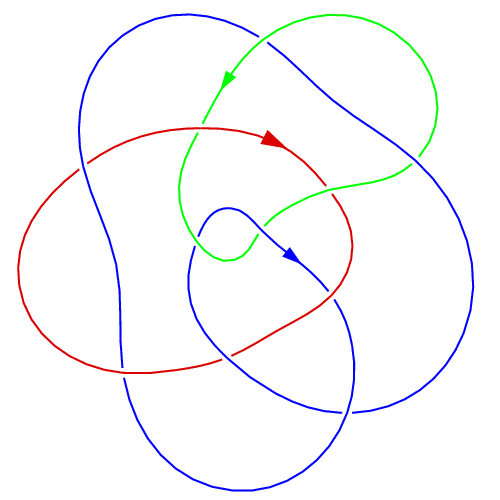
\includegraphics[width=\linewidth]{../data/link_mirror.png} 
            \subcaption{lustro $mL$}
        \end{minipage}
        \begin{minipage}[b]{.32\linewidth}
            \centering 
            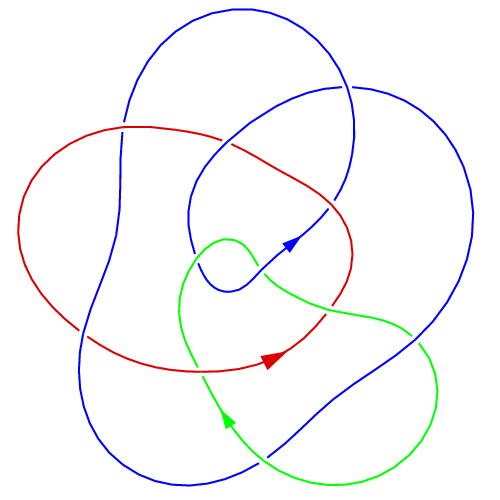
\includegraphics[width=\linewidth]{../data/link.png} 
            \subcaption{przykładowy splot $L$}
        \end{minipage}
        \begin{minipage}[b]{.32\linewidth}
            \centering 
            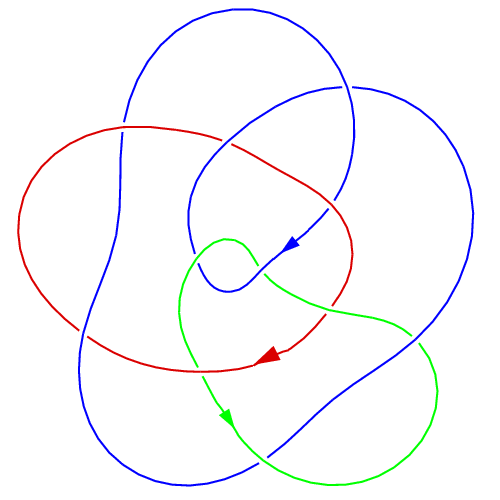
\includegraphics[width=\linewidth]{../data/link_reverse.png} 
            \subcaption{rewers $rL$}
        \end{minipage}
    \end{figure}
\end{definition}

Na lewym obrazku odbiliśmy diagram względem poziomej prostej,
ale równie dobrze można po prostu zamienić każde nadskrzyżowanie na podskrzyżowanie.
Zauważmy, że wykonując powyższe operacje na węźle możemy otrzymać mniej niż czterech różne obiekty
($L$, $mL$, $rL$, $mrL$) -- na przykład trójlistnik jest własnym rewersem, ale nie lustrem.

\begin{definition}
    Istnieje pięć typów symetrii węzłów:
    całkowicie chiralny albo skrętny (węzły $K$, $rK$, $mK$ są parami nierównoważne),
    odwracalny ($K \cong rK$),
    zwierciadlany ujemnie ($K \cong mrK$),
    zwierciadlany dodatnio ($K \cong mK$) oraz
    całkowicie zwierciadlany ($rK \cong K \cong mK$).
\end{definition}

Węzeł $9_{32}$ jest całkowicie skrętny. 
Ósemka jest zwierciadlana, trójlistnik jest odwracalny,
zaś $8_{17}$ to najprostszy przykład węzła nieodwracalnego.
Ten ostatni fakt jest jednak daleki od oczywistego -- 
sześćdziesiąt lat temu nie było pewne,
czy węzły nieodwracalne w ogóle istnieją.
W roku 1962 Ralph Fox wskazał kilku kandydatów do tego tytułu.
Hale Trotter odkrył rok później nieskończoną rodzinę nieodwracalnych precli (patrz \ref{def:pretzel}).
Obecnie wiadomo, że prawie wszystkie węzły są nieodwracalne (\cite[s.~46]{murasugi96}).
Wszystkie węzły torusowe są skrętne.

\begin{proposition}[Trotter, 1963] \label{trotter}
    Precel $(p, q, r)$, gdzie $p, q, r$ sa parami różnymi liczbami całkowitymi, nie jest odwracalny.
\end{proposition}

\begin{proof}
    Praca \cite{trotter63} sprowadza w elementarny sposób problem do pytania, czy pewna grupa posiada inwersję.
\end{proof}

Tait odnosił wrażenie, że zwierciadlane węzły mają parzysty indeks skrzyżowań,
ale Hoste (Thistlethwaite?) znalazł w 1998 kontrprzykład o piętnastu skrzyżowaniach.
Jest on jedynym znanym nam dzisiaj.
Hipoteza Taita jest prawdziwa dla węzłów pierwszych, alternujących.

Poniższa tabela oparta jest (kolejno) o ciągi 
\href{https://oeis.org/A051766}{51766}, 
\href{https://oeis.org/A051769}{51769}, 
\href{https://oeis.org/A051768}{51768}, 
\href{https://oeis.org/A051767}{51767}, 
\href{https://oeis.org/A052400}{52400}, 
z bazy danych ``The On-Line Encyclopedia of Integer Sequences'' (OEIS).

\begin{table}[h]
    \centering
    \begin{tabular}{@{}*{20}l@{}} \toprule
        skrzyżowania & 3 & 4 & 5 & 6 & 7 & 8 & 9 & 10 & 11 & 12 & 13 & 14 \\ \midrule
        całkowicie skrętne & 0 & 0 & 0 & 0 & 0 & 0 & 2 & 27 & 187 & 1103 & 6919 & 37885 \\
        odwracalne & 1 & 0 & 2 & 2 & 7 & 16 & 47 & 125 & 365 & 1015 & 3069 & 8813 \\
        $-$ zwierciadlane & 0 & 0 & 0 & 0 & 0 & 1 & 0 & 6 & 0 & 40 & 0 & 227 \\
        $+$ zwierciadlane & 0 & 0 & 0 & 0 & 0 & 0 & 0 & 0 & 0 & 1 & 0 & 6 \\
        zwierciadlane & 0 & 1 & 0 & 1 & 0 & 4 & 0 & 7 & 0 & 17 & 0 & 41 \\
        \bottomrule
        \hline
    \end{tabular}
    \caption{Liczba węzłów o poszczególnych typach symetrii}
    \label{tablica_wezlow}
\end{table}

% Koniec podsekcji Operacje na pojedynczym splocie

\subsection{Sumy wielu węzłów} % (fold)
\label{sub:knot_sum}
Suma spójna węzłów to szczególny przypadek sklejenia dwóch rozmaitości wzdłuż brzegu.

\begin{definition}
    Niech $L_1, L_2$ będą splotami.
    Ich \textbf{sumą niespójną}, $L_1 \sqcup L_2$,
    jest teoriomnogościowa suma rozłączna splotów
    $L_1$ i $L_2$ leżących po różnych stronach pewnej płaszczyzny.
\end{definition}

\begin{definition}
    Nacinając dwa zorientowane węzły w dwóch bliskich punktach i 
    ponownie zszywając je dwoma łukami nieprzecinającymi już
    istniejących otrzymujemy \textbf{sumę spójną}, $K_1 \shrap K_2$.
    \[
        \begin{tikzpicture}[baseline=-0.65ex,scale=0.1]
        \begin{knot}[clip width=5, flip crossing/.list={5}, ignore endpoint intersections=false,]
            \strand[thick] (-3.5, -3.5) [in=down, out=up] to (3.5, 3.5);
            \strand[thick] (3.5, 3.5) [in=right, out=up] to (-4.5, 10);
            \strand[thick] (-4.5, 10) [in=up, out=left] to (-10, 3.5);
            \strand[thick] (-10, 3.5) to (-10, -3.5);
            \strand[thick] (-10, -3.5) [in=left, out=down] to (-4.5, -10);
            \strand[thick] (-4.5, -10) [in=down, out=right] to (3.5, -3.5);
            \strand[thick] (3.5, -3.5) [in=down, out=up] to (-3.5, 3.5);
            \strand[thick] (-3.5, 3.5) [in=left, out=up] to (4.5, 10);
            \strand[thick] (4.5, 10) [in=up, out=right] to (10, 3.5);
            \strand[thick, -Latex] (10, 3.5) to (10, -3.5);
            \strand[thick] (10, -3.5) [in=right, out=down] to (4.5, -10);
            \strand[thick] (4.5, -10) [in=down, out=left] to (-3.5, -3.5);
            \node at (0, -15) {$K_1$};
        \end{knot}
        \end{tikzpicture}
        \shrap
        \begin{tikzpicture}[baseline=-0.65ex,scale=0.1]
        \begin{knot}[clip width=5, flip crossing/.list={6}, ignore endpoint intersections=false,]
            \strand[thick] (-3.5, -3.5) [in=down, out=up] to (3.5, 3.5);
            %\strand[thick] (3.5, 3.5) [in=right, out=up] to (-4.5, 10);
            %\strand[thick] (-4.5, 10) [in=up, out=left] to (-10, 3.5);
            \strand[thick] (-10, -3.5) [in=left, out=up] to (0, 6.5);
            \strand[thick, Latex-] (-10, -3.5) [in=left, out=down] to (-4.5, -10);
            \strand[thick] (-4.5, -10) [in=down, out=right] to (3.5, -3.5);
            \strand[thick] (3.5, -3.5) [in=down, out=up] to (-3.5, 3.5);
            %\strand[thick] (-3.5, 3.5) [in=left, out=up] to (4.5, 10);
            %\strand[thick] (4.5, 10) [in=up, out=right] to (10, 3.5);
            \strand[thick] (10, -3.5) [in=right, out=up] to (0, 6.5);
            \strand[thick] (10, -3.5) [in=right, out=down] to (4.5, -10);
            \strand[thick] (4.5, -10) [in=down, out=left] to (-3.5, -3.5);
            %
            \strand[thick] (-3.5, 3.5) [in=left, out=up] to (0, 10);
            \strand[thick] (3.5, 3.5) [in=right, out=up] to (0, 10);
            \node at (0, -15) {$K_2$};
        \end{knot}
        \end{tikzpicture}
        =
        \begin{tikzpicture}[baseline=-0.65ex,scale=0.1]
        \begin{knot}[clip width=5, flip crossing/.list={5, 22, 23}, ignore endpoint intersections=false,]
            \strand[thick] (-18.5, -3.5) [in=down, out=up] to (-11.5, 3.5);
            \strand[thick] (-11.5, 3.5) [in=right, out=up] to (-19.5, 10);
            \strand[thick] (-19.5, 10) [in=up, out=left] to (-25, 3.5);
            \strand[thick] (-25, 3.5) to (-25, -3.5);
            \strand[thick] (-25, -3.5) [in=left, out=down] to (-19.5, -10);
            \strand[thick] (-19.5, -10) [in=down, out=right] to (-11.5, -3.5);
            \strand[thick] (-11.5, -3.5) [in=down, out=up] to (-18.5, 3.5);
            \strand[thick] (-18.5, 3.5) [in=left, out=up] to (-10.5, 10);
            \strand[thick] (-10.5, 10) [in=left, out=right] to (-5, 2);
            \strand[thick, -Latex] (-5, 2) to (-5+6, 2);
            \strand[thick] (5, 2) to (-5+6, 2);
            \strand[thick] (3, -2) to [in=left, out=right] (10.5, -10);
            \strand[thick, -Latex] (3, -2) to (0, -2);
            \strand[thick] (-5, -2) to (0, -2);
            \strand[thick] (-5, -2) [in=right, out=left] to (-10.5, -10);
            \strand[thick] (-10.5, -10) [in=down, out=left] to (-18.5, -3.5);
            %%%
            \strand[thick] (11.5, -3.5) [in=down, out=up] to (18.5, 3.5);
            \strand[thick] (-10 +15, 2) [in=left, out=right] to (15, 6.5);
            \strand[thick] (10.5, -10) [in=down, out=right] to (18.5, -3.5);
            \strand[thick] (18.5, -3.5) [in=down, out=up] to (11.5, 3.5);
            \strand[thick] (25, -3.5) [in=right, out=up] to (15, 6.5);
            \strand[thick] (25, -3.5) [in=right, out=down] to (19.5, -10);
            \strand[thick] (19.5, -10) [in=down, out=left] to (11.5, -3.5);
            \strand[thick] (11.5, 3.5) [in=left, out=up] to (15, 10);
            \strand[thick] (18.5, 3.5) [in=right, out=up] to (15, 10);
            %%%
            \node at (0, -15) {$K_1 \shrap K_2$};
        \end{knot}
        \end{tikzpicture}
        \]
\end{definition}

Uogólnieniem tego działania oraz 
(nieopisanej w naszej pracy) operacji \emph{plumbing}
jest suma Murasugiego, dobrze wyjaśniona w czwartym rozdziale \cite{kawauchi96}.

Ważna jest orientacja składników:
suma dwóch trójlistników może być,
w zależności od ich orientacji,
węzłem babskim\todo{nazewnictwo pochodzi od żeglarzy, nie matematyków} lub prostym.
Fox pokazał w 1952 roku,
że dopełnienia tych dwóch węzłów nie są homeomorficzne.
Suma przeciwnie skręconych trójlistników jest plastrowa
(definicja \ref{def:slice_knot}),
natomiast tak samo skręconych -- nie.

\begin{proposition}
    Suma spójna jest dobrze określonym działaniem.
\end{proposition}

Suma spójna nie jest dobrze określona dla splotów:
nie istnieje kanoniczny wybór, które składowe łączyć ze sobą.

\begin{proof}
    Niech dane będą węzły $K_1$ oraz $K_2$
    oraz dwa różne łuki $\gamma_1$, $\gamma_2$,
    których można użyć do konstrukcji sumy spójnej.
    Skurczmy $K_1$, przeciągnijmy najpierw przez łuk $\gamma_1$, a następnie wzdłuż węzła $K_2$.
    Teraz wystarczy odwrócić ten proces z $\gamma_2$ w miejscu $\gamma_1$.
\end{proof}

\begin{proposition}
    Suma spójna zorientowanych węzłów posiada następujące własności:
    \begin{enumerate}[leftmargin=*]
    \itemsep0em
        \item jest łączna:
        $(K_1 \shrap K_2) \shrap K_3 \simeq K_1 \shrap (K_2 \shrap K_3)$,
        \item jest przemienna:
        $K_1 \shrap K_2 \simeq K_2 \shrap K_1$,
        \item posiada element neutralny:
        $K_1 \shrap \MalyNieWezel \simeq \MalyNieWezel \shrap K_1 \simeq K_1$.
    \end{enumerate}
\end{proposition}

Prosty dowód tego faktu pozostawiamy Czytelnikowi.
Pokażemy za to, iż węzły z sumą spójną nie tworzą grupy -- brakuje elementów przeciwnych.

\begin{proposition}
    Jeśli $K \shrap L = \NieWezel$, to $K = L = \NieWezel$.
\end{proposition}

\begin{proof}[Niedowód]
    Technika ta zwana jest szwindlem Mazura.
    Załóżmy, że $K \shrap L = \NieWezel$ i dopuśćmy wyjątkowo węzły dzikie.
    Skonstruujmy sumę $K \shrap L \shrap K \shrap \ldots$,
    przy czym kolejne składniki powinny zmniejszać się,
    aby ich suma nadal była węzłem.
    Wtedy
    \begin{align*}
        K & \simeq K \shrap [(L \shrap K) \shrap (L \shrap K) \ldots] \\
         & \simeq (K \shrap L) \shrap (K \shrap L) \shrap \ldots
         \simeq \NieWezel \shrap \NieWezel \shrap \ldots
         \simeq \NieWezel.
    \end{align*}
    Analogicznie pokazujemy, że $L \simeq \NieWezel$.
\end{proof}

Później poznamy prawdziwy, oparty na topologii algebraicznej, dowód.
Połączymy fakty \ref{genus_one} oraz \ref{genus_sum}.

Półgrupę węzłów z operacją sumy spójnej można ulepszyć do grupy na dwa sposoby:
albo poprzez zmianę działania, w jakie jest wyposażona,
albo osłabiając definicję węzłów równoważnych.
Drugi pomysł jest dużo lepszy niż pierwszy.
Na początku lat pięćdziesiątych J. Millnor wprowadził do matematyki pojęcie zgodności
(z angielskiego \emph{concordance}), które zastąpiło zwykłą równoważność.
Element neutralny nowej grupy to węzły plastrowe, ich opis leży w sekcji \ref{sec:slice}.
Zagadnienia te zakorzenione są w czterowymiarowej topologii.

% Koniec podsekcji Sumy wielu węzłów

% Koniec sekcji Operacje na węzłach

\section{Węzły pierwsze}
\label{sec:prime_knots}
Istnieje węzłowy odpowiednik liczb pierwszych.
Jest on ściśle związany z~podaną wyżej operacją sumy spójnej.
Do jego dostatecznie dobrego zrozumienia wymagana jest znajomość powierzchni Seiferta (opisanych w~sekcji \ref{sec:genus}).

\begin{definition}
    \label{primeknot}
    \index{węzeł!pierwszy}
    Nietrywialny węzeł nazywamy \textbf{pierwszym},
    kiedy nie można przedstawić go jako sumy spójnej $K_1 \shrap K_2$
    dwóch nietrywialnych węzłów $K_1, K_2$ (nie jest złożony).
\end{definition}

Okazuje się, że jeśli alternujący splot nie jest pierwszy,
to każdy jego alternujący diagram jest złożony.
Jako pierwszy fakt ten został wykazany przez Menasco w~\cite{menasco84}.
Dowód opiera się na multiplikatywności wielomianu BLM/Ho (opisuje go definicja \ref{def:blm_ho}).

Czy węzłów pierwszych jest nieskończenie wiele?
Tak (patrz fakt \ref{infty_primes}), potrafimy nawet oszacować liczbę $K_n$ węzłów pierwszych oraz $L_n$ splotów pierwszych.
W roku 1987 C. Ernst, D. Sumners w~oparciu o~wyniki Thistlethwaite'a, Kauffmana, oraz Murasugiego dotyczące węzłów alternujących pokazali w~\cite{ernst87}, że $K_n \ge \frac 1 3 (2^{n- 2} - 1)$, przy czym węzły lustrzane traktowane są jako różne.
Dokładniej:

\begin{proposition}
    Niech $f(n)$ oznacza liczbę węzłów dwumostowych o indeksie skrzyżowaniowym $n$.
    Wtedy
    \begin{equation}
        f(n) = \begin{cases}
        \frac 13 (2^{n-2} - 1) & \text{dla } n = 2k \ge 4 \\
        \frac 13 (2^{n-2} + 2^{(n-1)/2}) & \text{dla } n = 4k + 1 \ge 5 \\
        \frac 13 (2^{n-2} + 2^{(n-1)/2} + 2) & \text{dla } n = 4k + 3 \ge 7
        \end{cases}
    \end{equation}
\end{proposition}


Welsh rozpatruje w \cite{welsh92} węzły bez orientacji i znajduje poniższe ograniczenia.
Nie wiadomo, czy zwykłe granice istnieją.
\begin{equation}
    2.68 \le \liminf_{n \to \infty}  \sqrt[n]{K_n} \le \limsup_{n \to \infty} \sqrt[n]{L_n} \le \frac {27}{2}.
\end{equation}

% "On the number of knots and links" (MR1218230)

Czy niewęzeł nie daje się zapisać jako suma dwóch innych węzłów?
Byłoby to skrajnie niepożądane, gdyż każdy węzeł jest naturalnie spójną sumą siebie oraz niewęzła.
Na szczęście przy pomocy powierzchni Seiferta można pokazać, że tak się nie dzieje (jest to wniosek \ref{no_inverses}).
Prawdziwe jest dużo mocniejsze stwierdzenie,
którego nie udowodnimy ze względu na niedostatecznie rozwinięty aparat matematyczny.
Należy o~nim myśleć jak o~analogonie zasadniczego twierdzenia arytmetyki.

\begin{theorem}[Schubert, 1949]
    \label{thm:schubert}
    Każdy różny od niewęzła węzeł rozkłada się jednoznacznie na węzły pierwsze
    (jeśli tylko pominąć kolejność składników).
\end{theorem}

Schubert podał geometryczny dowód oparty o powierzchnie Seiferta; wyraził go w języku PL-rozmaitości (\cite{schubert49}), ale niedużym wysiłkiem można dokonać adaptacji do gładkiego świata.
Praca Schuberta korzysta z twierdzenia Alexandera, że 2-sfera w przestrzeni $\R^3$ ogranicza dysk, i jego odpowiednika dla torusów w $S^3$

My pokażemy tylko, że rozkład istnieje i jest skończony, to fakt \ref{genus_sum}.
% koniec sekcji Węzły pierwsze

\section{Niezmienniki liczbowe}
Jak wspomnieliśmy na początku rozdziału, sprawdzenie,
czy dwa diagramy przedstawiają sploty równoważne,
jest uciążliwym i~czasochłonnym zadaniem.
Aby je uprościć, podamy opis kilku prostych niezmienników o~całkowitych wartościach.
Zachodzą implikacje:
sploty równoważne $\Rightarrow$ ta sama wartość niezmiennika
oraz różne wartości niezmiennika $\Rightarrow$ różne sploty.

\subsection{Indeks skrzyżowaniowy} % (fold)
\label{sub:crossing_number}
\index{indeks!skrzyżowaniowy}
Z angielskiego \emph{crossing number}.

\begin{definition}
    Indeks skrzyżowaniowy $\operatorname{cr}(L)$ splotu $L$ to
    minimalna liczba skrzyżowań widocznych na diagramie,
    który przedstawia splot $L$.
\end{definition}

Jeśli $K_1, K_2$ są alternującymi węzłami o~$c_1, c_2$ skrzyżowaniach, to istnieje alternujący diagram ich sumy $K_1 \shrap K_2$ o~$c_1 + c_2$ skrzyżowaniach.
Lackenby w~pracy \cite{lackenby09} pokazał, że dla pewnej stałej $N \le 152$ zachodzi
\[
    \frac 1 N \sum_{i=1}^n \operatorname{cr} K_i \le \operatorname{cr} \left(\bigshrap_{i=1}^n K_i\right) \le \sum_{i=1}^n \operatorname{cr} K_i.
\]
(Tylko pierwsza nierówność jest ciekawa).
Jego argumentu (wykorzystującego powierzchnie normalne) nie można poprawić tak, by otrzymać stałą $N = 1$.
Wiadomo jednak, że indeks skrzyżowaniowy jest addytywny dla niektórych klas węzłów: alternujących (\cite{kauffman88}), adekwatnych\footnote{Węzły adekwatne nie pojawiają się na żadnej innej stronie tej książki.} czy torusowych (\cite{gruber03}).

\begin{theorem}[Bankwitz, 1930] \label{thm:bankwitz}
    Wyznacznik węzła alternującego jest nie mniejszy od jego indeksu skrzyżowaniowego.
\end{theorem}

\begin{proof}
    Pierwszy dowód podał Bankwitz w~pracy \cite{bankwitz30}.
    Inne rozumowanie przedstawił Crowell w~(łatwo dostępnym) artykule o~niespodziewanym tytule Nonalternating links z~1957 r.
\end{proof}

% Koniec podsekcji Indeks skrzyżowaniowy

\subsection{Liczba gordyjska} % (fold)
\label{sub:unknotting_number}
\index{liczba!gordyjska}
Z angielskiego \emph{unknotting number}.

\begin{definition}
    Liczba gordyjska $\operatorname{u}(K)$ węzła $K$ to minimalna liczba skrzyżowań,
    które trzeba odwrócić na pewnym jego diagramie, by dostać niewęzeł.
    Liczba $u$ nie musi być osiągana przez diagram o~minimalnej liczbie skrzyżowań.
\end{definition}

Dotychczas wyznaczono liczbę gordyjską dla prawie wszystkich węzłów pierwszych o~co najwyżej dziesięciu skrzyżowaniach,
Cha i~Livingston podają następującą listę wyjątków:
$10_{11}$, $10_{47}$, $10_{51}$, $10_{54}$, $10_{61}$, $10_{76}$, $10_{77}$, $10_{79}$, $10_{100}$ (stan na rok 2008).
S. Bleiler odkrył w~\cite{bleiler84} fascynujący przykład wymiernego węzła $2$-gordyjskiego,
czego świadkiem nie może być diagram o~minimalnej liczbie skrzyżowań
(ponieważ, co jeszcze bardziej fascynujące, węzeł ten posiada tylko jeden diagram o~dziesięciu skrzyżowaniach z~trzema do odwrócenia).
Koduje go liczba $29/6$, w~tabeli węzłów figuruje jako $10_8$.
Stojmenow w~\cite{stoimenow01} pokazuje, że jeden węzeł może mieć kilka diagramów minimalnych,
z których tylko niektóre są świadkiem $1$-gordyjskości (są to między innymi $14_{36750}$ oraz $14_{36760}$.)

Coward, Lackenby dowiedli w~\cite{coward11}, że jeśli $K$ jest 1-gordyjski i~o genusie 1, to z~dokładnością do pewnej relacji równoważności, tylko jedna zmiana skrzyżowania rozwiązuje go; chyba że $K$ jest ósemką -- wtedy takie zmiany są dwie.
Kanenobu, Murakami oraz Kohn dwadzieścia lat wcześniej wiedzieli, że wymierne sploty 1-gordyjskie posiadają rozwiązujące skrzyżowanie na minimalnym diagramie (\cite{kanenobu86}, \cite{kohn91}).

Jeśli odwrócenie pewnych skrzyżowań daje niewęzeł, to odwrócenie pozostałych także.
To daje proste, choć niezbyt pomocne oszacowanie liczby gordyjskiej: $2 \operatorname{u} (K) \le \operatorname{cr} (K)$.
Borodzik oraz Friedl podali niedawno całkiem mocne ograniczenia na liczbę gordyjską w~pracach \cite{borodzik14} i~\cite{borodzik15} opierając się o~parowanie Blanchfielda
(poprawiając ograniczenia z~sygnatury Levine'a-Tristrama, indeksu Nakanishiego oraz przeszkodą Lickorisha).
Dwadzieścia pięć węzłów o~co najwyżej dwunastu skrzyżowaniach ma liczbę gordyjską równą co najmniej trzy, co trudno pokazać innymi metodami.

Dla każdego nietrywialnego splotu istnieje diagram wymagający odwrócenia dowolnie wielu skrzyżowań (dowód zawiera praca \cite{taniyama09} Taniyamy).
Pokazany jest tam jeszcze jeden godny uwagi fakt.
Jeśli liczba gordyjska diagramu $D$ wynosi $\frac 12 (c(D) - 1)$,
co jest maksymalną możliwą wartością zgodnie z~naszym prostym ograniczeniem,
to węzeł jest $(2,p)$-torusowy albo wygląda jak diagram niewęzła po pierwszym ruchu Reidemeistera.

% Liczba gordyjska nietrywialnego węzła skręconego (definicja \ref{twist_knots}) to jeden, wystarczy bowiem rozwiązać jego splecione końce.
Patrz także stwierdzenie \ref{torus_unknotting}.

Suma dwóch węzłów $1$-gordyjskch jest $2$-gordyjska, pokazał to Scharleman.
Od początku teorii węzłów podejrzewano dużo więcej:

\begin{conjecture}
    Niech $K, J$ będą węzłami.
    Wtedy $u(K \shrap J) = u(K) + u(J)$, czyli liczba gordyjska jest addytywna.
\end{conjecture}

Z tej nieudowodnionej do dzisiaj (stan na 2018) hipotezy można wyciągnąć wniosek,
że jeśli do rozwiązania węzła wystarcza odwrócenie skrzyżowania, to jest pierwszy.
Podejrzewał to H. Wendt w~1937 roku,
kiedy policzył liczbę gordyjską węzła babskiego używając homologii rozgałęzionego nakrycia cyklicznego.

\begin{proposition}
    Węzły $1$-gordyjskie są pierwsze.
\end{proposition}

\begin{proof}[Niedowód]
    W pracy \cite{scharleman85} z~1985 roku M. Scharleman podał dość zawiłe uzasadnienie, w~które zamieszane były grafy planarne.
\end{proof}

W pracy \cite{shimizu14} Ayaka Shimizu pokazuje przykład innej operacji rozwiązującej węzły, ale nie wszystkie sploty:
zmianę skrzyżowań wokół obszaru na diagramie.

Liczbę gordyjską można uogólnić w naturalny sposób do metryki.
Mianowicie mając dane dwa węzły $K_0, K_1$, rozpatrzmy wszystkie homotopie $f : [0,1] \times S^1 \to \R^3$ takie, że wszystkie funkcje $f_t$ są zanurzeniami z co najwyżej jednym punktem podwójnym.
Zażądajmy dodatkowo, by styczne do krótkich łuków, które przecinają się w tym punkcie, były od siebie różne.
Odległością gordyjską między węzłami $K_0, K_1$ jest minimalna liczba podwójnych punktów, jakie posiada homotopia $f$.

Przestrzeń węzłów z~tą metryką bywa sprzeczna z~intuicją: twierdzenie C~z~pracy \cite{gambaudo05} głosi, że zawiera ona prawie idealną kopię przestrzeni euklidesowej dowolnego wymiaru.
Dokładniej:

\begin{proposition}
    Dla każdej liczby całkowitej $d \ge 1$ istnieje funkcja $\xi: \Z^d \to \mathcal{K}$, dodatnie stałe $A, B, C$ oraz norma $\|\cdot\|$ na przestrzeni $\R^d$ takie, że spełniona jest podwójna nierówność
    \[
        A\|x-y\|  - B \le d(\xi(x), \xi(y)) \le C\|x-y\|.
    \]
\end{proposition}

Dowód korzysta z grup warkoczowych, które poznamy w sekcji \ref{sec:braid}.

\begin{conjecture}[Bernhard 1994, Jablan 1998] \label{bernhard_jablan}
    Każdy węzeł $K$ posiada diagram $D$ realizujący liczbę gordyjską oraz skrzyżowanie, którego odwrócenie daje nowy węzeł $K'$ z diagramem $D'$ o mniejszej liczbie gordyjskiej: $u(D') < u(D)$.
\end{conjecture}

Gdyby hipoteza była prawdziwa, mielibyśmy dość prosty algorytm do wyznaczania liczby gordyjskiej $u(K)$: wystarczy skonstruować skończenie wiele diagramów minimalnych dla węzła $K$, odwracać kolejne skrzyżowania i szukać rekursywnie liczb gordyjskich nowych węzłów.
Hipoteza jest prawdziwa dla węzłów do jedenastu skrzyżowań (patrz baza danych KnotInfo C. Livingstona) i splotów o dwóch składowych do dziewięciu skrzyżowań, pokazał to Kohn w pracy \cite{kohn93} z 1993 (!) roku.
Brittenham, Hermiller twierdzą, że hipoteza jest fałszywa.

% Koniec podsekcji Liczba gordyjska

\subsection{Liczba mostowa} % (fold)
\label{sub:bridge_index}
\index{liczba!mostowa}
Z angielskiego \emph{bridge number}.
Wprowadzona w~1954 przez Schuberta.
\begin{definition}
    Liczba mostowa $\operatorname{br}(K)$ to minimalna liczba mostów:
    długich łuków, które biegną przez nadskrzyżowania.
\end{definition}

Można pokazać, że $n$-mostowe węzły rozkładają się na sumę dwóch trywialnych $n$-supłów.

\begin{proposition}
    Niech $K_1, K_2$ będą węzłami.
    Wtedy $\operatorname{br} (K_1) + \operatorname{br}(K_2) = \operatorname{br}(K_1 \# K_2) + 1$.
\end{proposition}

\begin{proof}[Nieedowód]
    Schubert pokazał to blisko pół wieku temu w~\cite{schubert54}.
    Nowszy dowód pochodzi od Schultensa, w~artykule \cite{schultens03} skorzystał z~foliacji na brzegu węzła towarzyszącego sateltarnemu.
    Dokładniejszy opis powyższych prac wykraczałby poza zakres tego opracowania, zostanie więc pominięty.
\end{proof}

Tylko jeden węzeł jest jednomostowy, to niewęzeł.
Kolejne w~hierarchii skomplikowania, czyli dwumostowe,
to domknięcia wymiernych supłów, patrz fakt \ref{prp:two_bridge_tangle}.
Węzły trójmostowe pozostają nie do końca zbadane.

\begin{conjecture}
    Jeśli $K$ jest węzłem, to $c(K) \ge 3 br(K) - 3$, przy czym równość zachodzi dokładnie dla niewęzła, trójlistnika i~sumy spójnej trójlistników (rozdział 4.3 z~podręcznika \cite{murasugi96}).
\end{conjecture}

Nie istnieje związek między liczbą mostową oraz gordyjską.
Po pierwsze, węzły torusowe $T_{2,n}$ są dwumostowe, a~ich liczba gordyjska jest duża.
Po drugie, podwojenie węzła (poza specjalnymi przypadkami, jak pokazał Schubert) zwiększa liczbę mostową dwukrotnie; liczba gordyjska takiego podwojenia wynosi $1$.
Podobnie nie ma zależności między liczbą mostową oraz genusem.

% Koniec podsekcji Liczba mostowa

\subsection{Liczba warkoczowa} % (fold)
\label{sub:braid_number}
\index{liczba!warkoczowa}
Z angielskiego \emph{braid number}.
Do jej określenia potrzebna jest definicja \ref{braid_def}.

\begin{definition}
    Liczba warkoczowa to minimalna liczba pasm, na których można zbudować warkocz, którego domknięciem jest wyjściowy węzeł.
\end{definition}

\begin{proposition}
    Węzeł o~$n$ skrzyżowaniach można zapleść na $n - 1$ pasmach.
\end{proposition}

Indeks warkoczowy zależy od orientacji ogniw i~trudno się go wyznacza w~ogólnym przypadku.
Poniższy dowód zakłada znajomość warkoczy (rozdział piąty).

\begin{proposition}
    Indeksem warkoczowym węzła torusowego $K(q, r)$, $rq \neq 0$, jest $\min\{|q|, |r|\}$.
\end{proposition}

\begin{proof}
    Niech $K$ będzie węzłem torusowym typu $(q,r)$ z~minimalnym przedstawieniem jako warkocz $\beta$.
    Z konstrukcji domknięcia (czyli dołączenia rozłącznych półokręgów) wynika,
    że diagram $K$ ma dokładnie $b(K)$ lokalnych maksimów.
    Definicja indeksu mostowego orzeka, iż $br(K) \le b(K)$.
    Bez straty ogólności niech $q > r > 0$.
    Skoro węzeł $K$ powstaje z~$r$-warkocza $(\sigma_{r-1} \ldots \sigma_2\sigma_1)^q$,
    indeks $b(K)$ nie przekracza $r = br(K)$.

    Skorzystaliśmy z~faktu \ref{torus_bridge}.
\end{proof}

% Koniec podsekcji Liczba warkoczowa

\subsection{Indeks zaczepienia} % (fold)
\label{sub:linking_number}
\begin{definition} \label{sign_def}
    Na diagramie zorientowanego splotu, każdemu skrzyżowaniu przypisujemy \textbf{znak} równy $\pm 1$.
    Skrzyżowania dodatnie nazywamy praworęcznymi, ujemne zaś: leworęcznymi.
    \[
        \sign \Bigl(\,\,\begin{tikzpicture}[baseline=-0.65ex,scale=0.07]
        \begin{knot}[clip width=5]
        \strand[semithick,-Latex] (-5,-5) -- (5,5);
        \strand[semithick,Latex-] (-5,5) -- (5,-5);
        \end{knot}\end{tikzpicture}\,\,\Bigr) = +1 \quad
        \sign \Bigl(\,\,\begin{tikzpicture}[baseline=-0.65ex,scale=0.07]
        \begin{knot}[clip width=5, flip crossing/.list={1}]
        \strand[semithick,-Latex] (-5,-5) -- (5,5);
        \strand[semithick,Latex-] (-5,5) -- (5,-5);
        \end{knot}\end{tikzpicture}\,\,\Bigr) = -1
    \]
\end{definition}

\begin{definition} \label{sign_def}
    \index{indeks!zaczepienia}
    Niech $L = K_1 \sqcup K_2$ będzie splotem o dwóch ogniwach.
    Wielkość
    \[
        \operatorname{lk}(K_1, K_2) = \frac 12 \sum_i \sign c_i,
    \]
    gdzie sumowanie rozciąga się na wszystkie skrzyżowania, gdzie spotykają się łuki z różnych ogniw, nazywamy \textbf{indeksem zaczepienia} węzłów $K_1, K_2$.
    Ogólniej, jeśli $L = K_1 \sqcup \ldots \sqcup K_n$ jest splotem o $n$ ogniwach, to jego indeks zaczepienia wyznacza wzór $\operatorname{lk}(L) = \sum_{i < j} \operatorname{lk}(K_i, K_j)$.
\end{definition}

Zauważmy, że indeks zaczepienia splotu Hopfa wynosi $1$, natomiast splotu Whiteheada $0$.
Są zatem istotnie różne.
W obydwu przypadkach indeks zaczepienia jest liczbą całkowitą, nie stanowi to przypadku.
Na mocy twierdzenia Jordana $\operatorname{lk}$ jest funkcją o całkowitych wartościach.

\begin{proposition}
    Indeks zaczepienia jest dobrze określonym niezmiennikiem zorientowanych splotów.
\end{proposition}

\begin{proof}
    Sprawdźmy wpływ ruchów Reidemeistera na wartość
    $\operatorname{lk}(L)$:

    \[
        \fbox{
        \begin{tikzpicture}[baseline=-0.65ex,scale=0.07]
        \begin{knot}[clip width=5]
        \strand[semithick] (-10,10) .. controls (-10,2) and (-10,2) .. (-6,-2);
        \strand[semithick] (-10,-10) .. controls (-10,-2) and (-10,-1) .. (-9,0);
        \strand[semithick] (-7,1) -- (-6,2);
        \strand[semithick] (-6,2) .. controls (2,9) and (2,-9) .. (-6,-2);
        \end{knot}
        \end{tikzpicture}
        $\stackrel{R_1}{\cong} \,\,$
        \begin{tikzpicture}[baseline=-0.65ex,scale=0.07]
        \begin{knot}[clip width=5]
        \strand[semithick] (0,10) -- (0,-10);
        \end{knot}
        \end{tikzpicture}}
        %%%
        \quad \fbox{
        \begin{tikzpicture}[baseline=-0.65ex,scale=0.07]
        \begin{knot}[clip width=5]
        \strand[semithick] (4,-10) .. controls (4,-4) and (-4,-4) .. (-4,0);
        \strand[semithick] (4,10) .. controls (4, 4) and (-4, 4) .. (-4,0);
        \strand[semithick] (-4,-10) .. controls (-4,-4) and (4,-4) .. (4,0);
        \strand[semithick] (-4,10) .. controls (-4, 4) and (4,4) .. (4,0);
        \node[blue] at (-4,4)[left] {$a$};
        \node[blue] at (-4,-4)[left] {$-a$};
        \end{knot}
        \end{tikzpicture}
        $\stackrel{R_2}{\cong} \,\,$
        \begin{tikzpicture}[baseline=-0.65ex,scale=0.07]
        \begin{knot}[clip width=5]
        \strand[semithick] (4,-10) .. controls (4,-4) and (1,-4) .. (1,0);
        \strand[semithick] (4,10) .. controls (4, 4) and (1, 4) .. (1,0);
        \strand[semithick] (-4,-10) .. controls (-4,-4) and (-1,-4) .. (-1,0);
        \strand[semithick] (-4,10) .. controls (-4, 4) and (-1,4) .. (-1,0);
        \end{knot}
        \end{tikzpicture}}
        %%%
        \quad \fbox{
        \begin{tikzpicture}[baseline=-0.65ex,scale=0.07]
        \begin{knot}[clip width=5, flip crossing/.list={1,2,3}]
        \strand[semithick] (-10,-10) -- (10,10);
        \strand[semithick] (-10,10) -- (10,-10);
        \strand[semithick] (-10,-2) .. controls (-4, -2) and (-4,8) .. (0,8);
        \strand[semithick] (10,-2) .. controls (4, -2) and (4,8) .. (0,8);
        \node[blue] at (-6,4)[left] {$a$};
        \node[blue] at (6,4)[right] {$b$};
        \node[blue] at (0,-2)[below] {$c$};
        \end{knot}
        \end{tikzpicture}
        $\stackrel{R_3}{\cong} \,\,$
        \begin{tikzpicture}[baseline=-0.65ex,scale=0.07]
        \begin{knot}[clip width=5, flip crossing/.list={1,2,3}]
        \strand[semithick] (-10,-10) -- (10,10);
        \strand[semithick] (-10,10) -- (10,-10);
        \strand[semithick] (-10,2) .. controls (-4, 2) and (-4,-8) .. (0,-8);
        \strand[semithick] (10,2) .. controls (4, 2) and (4,-8) .. (0,-8);
        \node[blue] at (-6,-4)[left] {$a$};
        \node[blue] at (6,-4)[right] {$b$};
        \node[blue] at (0,2)[above] {$c$};
        \end{knot}
        \end{tikzpicture}}
    \]
    Na mocy twierdzenia Reidemeistera dowód został zakończony.
\end{proof}

Kawauchi definiuje jeszcze \emph{twisting number}: sumę spinów po wszystkich składowych.

% Koniec podsekcji Indeks zaczepienia

\subsection{Sygnatura} % (fold)
\label{sub:signature}
\index{sygnatura}
Sygnatura pojawia się w~fakcie \ref{slice_signature}.

\begin{definition}
    Sygnatura to niezmiennik topologiczny zadany (kłębiastą) relacją rekurencyjną:
    \begin{itemize}[leftmargin=*]
    \itemsep0em
        \item $\sigma (\LittleUnknot) = 0$,
        \item $\sigma (K_+) - \sigma (K_-) \in \{0, 2\}$,
        \item $4 \mid \sigma (K)$ wtedy i~tylko wtedy, gdy $\nabla(2i) > 0$ (wielomian Conwaya).
    \end{itemize}
\end{definition}

\begin{proposition} \label{prop_sigma_inverse}
    Mamy $\sigma(K^*) = -\sigma(K)$ oraz $\sigma(-K) = \sigma(K)$.
\end{proposition}

\begin{proof}
    To jest twierdzenie 6.4.5 z podręcznika \cite{murasugi96}.
\end{proof}

\begin{proposition} \label{prop_sigma_additive}
    Sygnatura jest addytywna: $\sigma(K_1 \shrap \ldots \shrap K_n) = \sum_{k=1}^n \sigma(K_k)$.
\end{proposition}

Węzły achiralne mają zerową sygnaturę, zatem trójlistnik nie jest achiralny.
Z faktów \ref{prop_sigma_inverse} oraz \ref{prop_sigma_additive} wynika, że suma tak samo skręconych trójlistników nie jest achiralna ($\sigma = \pm 4$), natomiast węzeł prosty (suma różnie skręconych) ma zerową sygnaturę i jak można przekonać się ze standardowego diagramu, jest achiralny.

Sygnatura pozwala uzyskać proste oszacowanie liczby gordyjskiej od dołu:

\begin{proposition}
    Mamy $2 u(K) \ge |\sigma(K)|$.
\end{proposition}

\begin{proof}
    To jest twierdzenie 6.4.8 z podręcznika \cite{murasugi96}.
\end{proof}

Nie istnieje bezpośredni związek między sygnaturą i~liczbą mostową.
Węzeł torusowy $T_{2,n}$ jest dwumostowy, jego sygnatura wynosi $n - 1$.
Suma spójna węzłów prostych ma zerową sygnaturę i~nieograniczoną liczbę mostową.
Wynika to z~ogólniejszego faktu:


Czy istnieje węzeł o~sygnaturze $4$ i~wyznaczniku postaci $n = 4k + 1$ dla $k$ całkowitego dodatniego?
Stojmenow twierdzi, że jeśli tak jest, to wszystkie pierwsze dzielniki $n$ dają resztę $1$ z~dzielenia przez $24$ i~są większe od $2857$.

% Koniec podsekcji Sygnatura

\subsection{Liczba patykowa} % (fold)
\label{sub:stick_index}
\index{liczba!patykowa}
Z angielskiego \emph{stick index}.

\begin{definition}
    Liczba patykowa $\operatorname{s}(K)$ to minimalna liczba odcinków w~łamanej, która przedstawia węzeł.
\end{definition}

Liczba patykowa niewęzła to $3$, sumy spójnej $n$ trójlistników to $2n+4$ (wynik z~\cite{greilsheimer97}).
Negami pokazał w~\cite{negami91}, że prawdziwe są nierówności
\[
    \frac{5+\sqrt{9 + 8 \operatorname{cr} K}}{2} \le \operatorname{s} K \le 2 \operatorname{cr} K
\]
Nie jest znany węzeł realizujący dolne ograniczenie, górne realizuje trójlistnik.
W 2010 roku Huh oraz Oh poprawili górne ograniczenie do $3/2(\operatorname{cr} K+1)$ (pomijając niewęzeł, patrz \cite{huh11}).
Dla węzłów torusowych znamy dokładne wartości: jeśli $2 \le p < q \le 2p$, to $\operatorname{s} T_{p,q} = 2q$ oraz $\operatorname{s} T_{p, p-1} = 2p$ (dowód pierwszej równości w~\cite{jin97}).

% Koniec podsekcji Liczba patykowa

\subsection{Długość sznurowa} % (fold)
\label{sub:ropelength}
Długość sznurowa, z~angielskiego \emph{ropelength}, pochodzi z~fizycznej teorii węzłów, która bierze pod uwagę obiekty wykonane z~nieelastycznych materiałów

Długość sznurowa $L$ to stosunek długości węzła do jego grubości $\tau$ (mówimy, że węzeł $K$ jest grubości $\tau$, jeśli ma otoczenie rurowe bez samoprzecięć z~przekrojem poprzecznym o~promieniu $\tau$).
Przez wiele lat zastanawiano się, czy można zawiązać węzeł ze sznura o~długości jednej stopy i~promieniu jednego cala.
Nie jest to możliwe: rozumowanie oparte o~czterosieczne pokazuje, że długość sznurowa nietrywialnego węzła wynosi co najmniej $15.66$ (dla trójlistnika jest to co najmniej $16.372$).

Węzeł realizujący długość sznurową jest klasy $C^1$.

Prawdziwe są oszacowania asymptotyczne:
\[
    L = \Omega (\operatorname{cr}^{3/4}),  \quad
    L = O(\operatorname{cr} \log^5 \operatorname{cr})
\]

% Koniec podsekcji Ropelength

% Koniec sekcji Niezmienniki liczbowe


\chapter{Niezmienniki kolorowe}
Opisane w pierwszym rozdziale niezmienniki, takie jak liczba gordyjska czy liczba mostowa, pozwalają na odróżnienie od siebie niektórych węzłów, jednak wyznaczanie ich wartości nie jest łatwym zadaniem.
Dlatego nie potrafimy jeszcze uzasadnić, że istnieje jakikolwiek nietrywialny węzeł.
Zmieni się to teraz: poznamy kolorowania, niezmienniki splotów powstałe z diagramów, gdzie każde włókno występuje w jednym z trzech kolorów.

Następnie rozszerzymy paletę z trzech do skończenie wielu kolorów, by później zastąpić ją dowolną nieprzemienną grupą skończoną.
Nawet ten ostatni wariant kolorowania nie stanowi idealnego narzędzia do klasyfikacji węzłów.
Mówimy, że nie jest zupeły: istnieją różne węzły, którym przypisuje te same wartości, czyli ich nie odróżnia.
Problem ten będzie powtarzać się dla prawie wszystkich późniejszych niezmienników, z wyjątkiem dopiero całki Koncewicza (patrz sekcja \ref{sec:vassiliev}).

\section{Kolorowanie splotów} % (fold)

Przygodę z kolorowaniami rozpoczyna się zazwyczaj od trójkolorowalności.
Jest to pewna cecha diagramów, którą można posiadać albo nie.

\begin{definition}[trójkolorowalność]
    Niech $D$ będzie diagramem splotu $L$, którego łuki występują w~trzech kolorach.
    Jeżeli spełnione są następujące warunki:
    \begin{itemize}[leftmargin=*]
        \item nie wszystkie łuki są tego samego koloru,
        \item przy każdym skrzyżowaniu spotykają się albo trzy łuki w trzech różnych kolorach, albo wszystkie tego samego koloru,
    \end{itemize}
    to mówimy, że diagram $D$ jest trójkolorowalny.
\end{definition}

 Splot posiadający trójkolorowalny diagram nazywamy krótko trójkolorowalnym.

\begin{example}
    Trójlistnik jest trójkolorowalny, niewęzeł nie jest.
    Węzły te są zatem od siebie różne.
\end{example}

Dla własnej wygody jako kolorów używać będziemy kolejnych liczb naturalnych $0, 1, \ldots, n$.
Pozwala to zapisać warunek kolorowalności równaniem algebraicznym, niezależnie od ilości użytych kolorów.

\begin{definition}[kolorowanie]
    \label{def:colouring_equation}
    Niech $L$ będzie splotem, zaś $n$ liczbą naturalną.
    Mówimy, że splot $L$ jest kolorowalny modulo $n$, jeśli posiada diagram, którego włóknom można przypisać liczby całkowite $0, \ldots, n - 1$ tak, by
    \begin{enumerate}[leftmargin=*]
        \item istniały dwa włókna różnych kolorów,
        \item równanie $a + b \equiv 2c$ modulo $n$ było spełnione przy każdym skrzyżowaniu:
    \end{enumerate}
\begin{comment}
    \[
        \begin{tikzpicture}[baseline=-0.65ex, scale=0.12]
            \useasboundingbox (-5, -5) rectangle (5,5);
            \begin{knot}[clip width=5, end tolerance=1pt, flip crossing/.list={1}]
                \strand[semithick] (-5,5) to (5,-5);
                \strand[semithick] (-5,-5) to (5,5);
                \node[darkblue] at (5, 5)[below right] {$c$};
                \node[darkblue] at (5, -5)[above right] {$b$};
                \node[darkblue] at (-5, 5)[below left] {$a$};
            \end{knot}
        \end{tikzpicture}.
    \]
\end{comment}
    Takie przyporządkowanie nazywamy kolorowaniem.
\end{definition}

Metoda ta została odkryta razem z~uogólnieniem do $n$ kolorów przez Ralpha Foxa w~1956, kiedy próbował uczynić teorię węzłów bardziej przystępną dla studentów.
Opierając się na definicji oraz ruchach Reidemeistera możemy wykazać pierwsze własności kolorowań.

Kolorowanie nazywamy trywialnym, jeśli używa tylko jednego koloru.

\begin{proposition}
    \label{prp:colouring_invariance}
    Własność ,,być $n$-kolorowalnym'' jest niezmiennikiem węzłów.
\end{proposition}

\begin{proof}
    Wystarczy sprawdzić, jak ruchy Reidemeistera zmieniają kolory.
    Pierwszy i~drugi:
\begin{comment}
    \[
        \fbox{
        \begin{tikzpicture}[baseline=-0.65ex,scale=0.07]
        \begin{knot}[clip width=5]
            \strand[semithick] (-10,10) .. controls (-10,2) and (-10,2) .. (-6,-2);
            \strand[semithick] (-10,-10) .. controls (-10,-2) and (-10,-1) .. (-9,0);

            \strand[semithick] (-7,1) -- (-6,2);
            \strand[semithick] (-6,2) .. controls (2,9) and (2,-9) .. (-6,-2);
            \node[darkblue] at (-10, 10)[below left] {$a$};
            \node[darkblue] at (-10, -10)[above left] {$b \equiv a$};
        \end{knot}
        \end{tikzpicture}
        $\stackrel{R_1}{\cong} \,\,$
        \begin{tikzpicture}[baseline=-0.65ex,scale=0.07]
        \begin{knot}[clip width=5]
            \strand[semithick] (0,10) -- (0,-10);
            \node[darkblue] at (0, 0)[left] {$a$};
        \end{knot}
        \end{tikzpicture}}
        %%%
        \quad \fbox{
        \begin{tikzpicture}[baseline=-0.65ex,scale=0.07]
        \begin{knot}[clip width=5]
            \strand[semithick] (4,-10) .. controls (4,-4) and (-4,-4) .. (-4,0);
            \node[darkblue] at (-4, -10)[above left] {$d \equiv b$};
            \strand[semithick] (4,10) .. controls (4, 4) and (-4, 4) .. (-4,0);
            \node[darkblue] at (4, 10)[below right] {$a$};
            \strand[semithick] (-4,-10) .. controls (-4,-4) and (4,-4) .. (4,0);
            \node[darkblue] at (4, 0) [right] {$c \equiv 2a-b$};
            \strand[semithick] (-4, 10) .. controls (-4, 4) and (4,4) .. (4,0);
            \node[darkblue] at (-4, 10) [below left] {$b$};
        \end{knot}
        \end{tikzpicture}
        $\stackrel{R_2}{\cong} \,\,$
        \begin{tikzpicture}[baseline=-0.65ex,scale=0.07]
        \begin{knot}[clip width=5]
            \strand[semithick] (4,-10) .. controls (4,-4) and (1,-4) .. (1,0);
            \strand[semithick] (4,10) .. controls (4, 4) and (1, 4) .. (1,0);
            \strand[semithick] (-4,-10) .. controls (-4,-4) and (-1,-4) .. (-1,0);
            \strand[semithick] (-4,10) .. controls (-4, 4) and (-1,4) .. (-1,0);
        \end{knot}
        \end{tikzpicture}}
    \]
\end{comment}
    Trzeci ruch także nie wymaga skomplikowanych rachunków.
    Najkrótszy łuk na diagramach ma kolor $2a-c$ po lewej oraz $2b-c$ po prawej stronie.
\begin{comment}
    \[
     \fbox{
        \begin{tikzpicture}[baseline=-0.65ex,scale=0.07]
        \begin{knot}[clip width=5, flip crossing/.list={1,2,3}]
            \node[darkblue] at (-10, 10) [above] {$b$};
            \node[darkblue] at (10, 10) [above] {$c$};
            \node[darkblue] at (-10, -10) [below] {$2a-2b+c$};
            \node[darkblue] at (10, -10) [below] {$2a-b$};
            \node[darkblue] at (-10, -2) [left] {$a$};
            \strand[semithick] (-10,-10) -- (10,10);
            \strand[semithick] (-10,10) -- (10,-10);
            \strand[semithick] (-10,-2) .. controls (-4, -2) and (-4,8) .. (0,8);
            \strand[semithick] (10,-2) .. controls (4, -2) and (4,8) .. (0,8);
        \end{knot}
        \end{tikzpicture}
        $\stackrel{R_3}{\cong} \,\,$
        \begin{tikzpicture}[baseline=-0.65ex,scale=0.07]
        \begin{knot}[clip width=5, flip crossing/.list={1,2,3}]
            \node[darkblue] at (-10, 10) [above] {$b$};
            \node[darkblue] at (10, 10) [above] {$c$};
            \node[darkblue] at (-10, -10) [below] {$2a-2b+c$};
            \node[darkblue] at (10, -10) [below] {$2a-b$};
            \node[darkblue] at (10, 2) [right] {$a$};
            \strand[semithick] (-10,-10) -- (10,10);
            \strand[semithick] (-10,10) -- (10,-10);
            \strand[semithick] (-10,2) .. controls (-4, 2) and (-4,-8) .. (0,-8);
            \strand[semithick] (10,2) .. controls (4, 2) and (4,-8) .. (0,-8);
        \end{knot}
        \end{tikzpicture}} \qedhere
    \]
\end{comment}
\end{proof}

Trójlistnik koloruje się dokładnie modulo krotności trójki, ósemka zaś -- piątki.
Sama kolorowalność nie mówi wiele, splot jest kolorowalny lub nie.
Dowód faktu \ref{prp:colouring_invariance} pokazuje coś więcej: liczba kolorowań, być może trywialnych, jest mocniejszym niezmiennikiem.

\begin{lemma}
    \label{lem:colouring_arc}
    Niech $D$ będzie diagramem z definicji \ref{def:colouring_equation} z wybranym łukiem, zaś $k \in \{0, \ldots, n - 1\}$ pewnym kolorem.
    Bez straty ogólności możemy założyć, że krótki łuk jest koloru $k$.
\end{lemma}

Kolorem tym zazwyczaj jest $0$.

\begin{proof}
    Dodanie tej samej wartości do wszystkich łuków na dobrze pokolorowanym diagramie daje nowy, także dobrze pokolorowany diagram.
\end{proof}

\begin{proposition}
    \label{prp:no_colourings_mod_2}
    Żaden węzeł nie koloruje się modulo dwa.
\end{proposition}

\begin{proof}
    Załóżmy nie wprost, że istnieje nietrywialne kolorowanie.
    Analiza czterech możliwych skrzyżowań pokazuje, że włókna wychodzące z~tunelu muszą mieć ten sam kolor.
    Przechodząc wzdłuż węzła widzimy jeden kolor, wbrew założeniu nie wprost.
\end{proof}

\begin{proposition}
    Każdy splot o co najmniej dwóch ogniwach koloruje się modula dwa.
\end{proposition}

\begin{proof}
    Wystarczy pomalować jedną składową zerem, a~pozostałe jedynkami.
\end{proof}

Sploty rozszczepialne są $n$-kolorowalne dla każdego $n \ge 2$, można skorzystać z~tego samego schematu kolorowania.
Pierścienie Boromeuszy nie kolorują się modulo trzy, nie są zatem rozszczepialne.
% TODO: pierścienie Boromeuszy nie są nigdzie zdefiniowane
Sploty, które nie są kolorowalne modulo $n$ dla każdej liczby $n \in \N$ nazywa się czasem niewidzialnymi, dwa węzły do dziesięciu skrzyżowań mają tę własność: $10_{124}$ oraz $10_{153}$.

Pokażemy teraz, że suma równań kolorujących z dobrze wybranymi znakami jest postaci $0 \equiv 0 \mod n$.
Będziemy potrzebować kilku pomocniczych definicji.
Każdy diagram węzła rozcina płaszczyznę na obszary, z~czego jeden jest nieograniczony.

\begin{definition}[uszachowienie]
    Przyporządkowanie każdemu z~obszarów, na jakie diagram rozcina płaszczyznę, jednego z~dwóch kolorów tak, by sąsiadujące ze sobą obszary były różnych kolorów, nazywamy uszachowieniem.
\end{definition}

Ustalmy węzeł $K$ oraz dowolne uszachowienie dla jego diagramu.
Skojarzmy z~każdym skrzyżowaniem równanie kolorujące, zgodnie z~poniższym schematem:
\begin{comment}
\[\begin{tikzpicture}[baseline=-0.65ex, scale=0.12]
    \useasboundingbox (-5, -10) rectangle (5,5);
    \begin{knot}[clip width=5, end tolerance=1pt, flip crossing/.list={1}]
        \strand[semithick] (-5,5) to (5,-5);
        \strand[semithick] (-5,-5) to (5,5);
        \fill[blue!20!white] (-4, 5) to (0, 1) to (4, 5);
        \fill[blue!20!white] (-4, -5) to (0, -1) to (4, -5);
        \node[darkblue] at (-5, -5)[left] {$a$};
        \node[darkblue] at (-5, +5)[left] {$b$};
        \node[darkblue] at (+5, -5)[right] {$c$};
        \node[darkblue] at (+5, +5)[right] {$a$};
        \node[darkblue] at (0, -10) {$+a-b+a-c=0 \mod n$};
    \end{knot}
    \end{tikzpicture}
    \quad\quad\quad\quad\quad\quad\quad\quad\quad\quad\quad\quad
    \begin{tikzpicture}[baseline=-0.65ex, scale=0.12]
    \useasboundingbox (-5, -10) rectangle (5,5);
    \begin{knot}[clip width=5, end tolerance=1pt, flip crossing/.list={1}]
        \strand[semithick] (-5,5) to (5,-5);
        \strand[semithick] (-5,-5) to (5,5);
        \fill[blue!20!white] (5, -4) to (1, 0) to (5, 4);
        \fill[blue!20!white] (-5, -4) to (-1, 0) to (-5, 4);
        \node[darkblue] at (-5, -5)[left] {$a$};
        \node[darkblue] at (-5, +5)[left] {$b$};
        \node[darkblue] at (+5, -5)[right] {$c$};
        \node[darkblue] at (+5, +5)[right] {$a$};
        \node[darkblue] at (0, -10) {$-a+b-a+c=0 \mod n$};
    \end{knot}
    \end{tikzpicture}
\]
\end{comment}

\begin{proposition}
    \label{prp:colouring_sum_zero}
    Sumą równań kolorujących o dobrze wybranych znakach jest $0 \equiv 0 \mod n$.
\end{proposition}

Będziemy potrzebować tego do pokazania, że wyznacznik determinuje kolorowalność splotu.

\begin{proof}
    Każde równanie kolorujące składa się z~czterech wyrazów, po jednym od każdej nici, która spotyka się w~danym skrzyżowaniu.
    Nić biegnie między dwoma skrzyżowaniami, więc suma wszystkich równań kolorujących składa się z~par składników, po jednej parze na nić.
    Składniki te są przeciwnych znaków, zatem wzajemnie się znoszą.
    Suma równań kolorujących jest sumą zer, a~to należało udowodnić.
\end{proof}

Liczbę kolorowań splotu $L$ modulo $n$, trywialnych lub nie, oznaczamy przez $\tau_n(L)$.

\begin{proposition}
    Jeśli $K, L$ są węzłami, to $3\tau_3(K \shrap L) = \tau_3(K)\tau_3(L)$.
\end{proposition}

\begin{corollary}
    Istnieje nieskończenie wiele węzłów.
\end{corollary}

\begin{proof}
    Suma spójna $n$ trójlistników ma $3^{n+1}$, trywialnych lub nie, $3$-kolorowań.
\end{proof}

Jako kolorów użyjemy teraz elementów $g_1, \ldots, g_n$ pewnej skończonej grupy $G$.

\begin{definition}[etykietowanie]
    Mówimy, że zorientowany węzeł $K$ jest etykietowalny grupą $G$ generowaną przez elementy $g_1, \ldots, g_n$, jeśli posiada diagram, którego włóknom przypisano elementy $g_1, \ldots, g_n$ tak, by równanie $gk=hg$ było spełnione przy każdym skrzyżowaniu ($g$: włókno biegnące górą, $k$: bo jego lewej stronie, $h$: po prawej).
\begin{comment}
    \[
        \begin{tikzpicture}[baseline=-0.65ex, scale=0.12]
            \useasboundingbox (-5, -5) rectangle (5,5);
            \begin{knot}[clip width=5, end tolerance=1pt, flip crossing/.list={1}]
                \strand[semithick] (-5,5) to (5,-5);
                \strand[semithick, -Latex] (-5,-5) to (5,5);
                \node[darkblue] at (5, 5)[below right] {$g$};
                \node[darkblue] at (5, -5)[above right] {$h$};
                \node[darkblue] at (-5, 5)[below left] {$k$};
            \end{knot}
        \end{tikzpicture}
    \]
\end{comment}
\end{definition}

Równanie $gkg^{-1}=h$ mówi, że etykiety włókien wchodzących oraz wychodzących są sprzężone.
Wynika stąd, że wszystkie etykiety pochodzą z~jednej klasy sprzężoności.
Muszą jednocześnie generować całą grupę, dlatego $G$ musi być grupą nieprzemienną lub trywialną.
Etykietowalność jest niezmiennikiem węzłów i~nie zależy od orientacji węzła:
jeżeli elementy $g_1, \ldots, g_n$ generują grupę, to ich odwrotności także.

Rozpatrzmy węzły $6_1$ oraz $9_{46}$ i~spróbujmy etykietować je transpozycjami z~grupy $S_4$.
Wybranie dwóch etykiet przy jednym skrzyżowaniu $6_1$ wymusza etykiety dla wszystkich włókien.
Dwie transpozycje nie mogą generować grupy $S_4$, natomiast włókna węzła $9_{46}$ dają się etykietować samymi transpozycjami.
Węzły te są więc różne, choć mają te same własności kolorujące.

Etykietowanie jest mocnym narzędziem odróżniającym węzły.
Thistlethwaite w 1985 roku korzystając z niego klasyfikował węzły o~co najwyżej 13 skrzyżowaniach (jest ich, jak ostatecznie się okazało, 12965).
Mają one tylko 5639 różnych wielomianów Alexandera, ale etykietowania trzynastoma różnymi grupami pozwoliły zmniejszyć liczbę nierozpoznanych węzłów do około tysiąca.
Wśród nich 30 posiada wielomian Conwaya $1 + 2z^2 + 2z^4$, ale pary rozróżniane wielomianem HOMFLY mają też różne wielomiany Jonesa.
Wielomiany opisujemy w~rozdziale trzecim.

Niech $p \ge 3$ będzie liczbą pierwszą, natomiast $D_p = \langle r, s \mid r^p = s^2 = e, rsr = s \rangle$ grupą diedralną rzędu $2p$.
Elementy tej grupy to $1, r, r^2, \ldots, r^{p-1}, s, sr, \ldots, sr^{p-1}$.
,,Obrót'' $r^k$ jest sprzężony tylko ze swoją odwrotnością, ale ,,symetrie osiowe'' $sr^k$ tworzą jedną klasę sprzężoności.
Łatwo widać, że dowolne dwie z~nich generują całą grupę $D_p$.

\begin{proposition}
    Węzeł $K$ jest $p$-kolorowalny wtedy i~tylko wtedy, gdy jest $D_p$-etykietowalny.
\end{proposition}

\begin{proof}
    Załóżmy, że $K$ ma $n$ włókien.
    Wiemy już, że każde $D_p$-etykietowanie wykorzystuje tylko elementy $sr^{a_1}, \ldots, sr^{a_n}$ dla $1 \le a_i \le p$.
    Jest ono prawidłowe dokładnie wtedy, gdy analogiczne kolorowanie liczbami $a_1, \ldots, a_n$ jest prawidłowe.
\end{proof}

Kolorowania definiowano kiedyś jako surjekcje $\rho \colon \pi \to D_{2n}$ z~grupy podstawowej.
Jak mówi prezentacja Wirtingera, grupa splotu generowana jest przez ścieżki z~punktu bazowego w~$S^3$ do brzegu rurowego otoczenia splotu, wokół południka i~znowu do bazowego punktu.
Fox zauważył, że z~surjektywności $\rho$ wynika, iż generatory mapują się na symetrie osiowe $sr^k$.
Ponieważ istnieje wzajemnie jednoznaczna odpowiedniość między generatorami grupy splotu oraz łukami diagramu, każdemu możemy przypisać liczbę całkowitą $k$.
Etykietowania są więc uogólnieniem kolorowań.
Rozumowanie, które przedstawiliśmy, prowadzi do prostej klasyfikacji grup, których można użyć do etykietowania.

\begin{proposition}
    Niech $K$ będzie węzłem, $\pi$ grupą podstawową jego dopełnienia, zaś $G$ dowolną grupą.
    Następujące warunki są równoważne: $K$ jest $G$-etykietowalny; istnieje surjekcja $\pi_1 \to G$.
\end{proposition}

Historycznie, prezentacja Wirtingera była pierwsza, zaś etykietowania odkryto później.

\begin{proposition}[Perko]
    Niech $K$ będzie węzłem etykietowalnym grupą $S_3$.
    Wtedy $K$ jest też etykietowalny grupą $S_4$.
\end{proposition}

Nie znam innych nietrywialnych faktów dotyczących etykietowań.

% Koniec sekcji Kolorowanie splotów

\section{Macierz i wyznacznik} % (fold)
\label{sec:colour_matrix}
Zajmiemy się teraz wyznacznikiem, pierwszym nieoczywistym niezmiennikiem splotów, który przypisuje każdemu pewną liczbę całkowitą.
Jest on blisko związany z kolorowaniem.
Zauważmy, że pierwszy ruch Reidemeistera usuwa zamknięte krzywe, czyli pojedyncze łuki bez skrzyżowań.
Diagram bez takich krzywych ma tyle samo skrzyżowań, co łuków.

\begin{definition}[macierz kolorująca]
    Ustalmy diagram bez zamkniętych krzywych dla splotu $L$ z łukami $x_0, \ldots, x_m$ oraz skrzyżowaniami $0, \ldots, m$.
    Definiujemy macierz $A$, której wyraz $a_{lj}$ jest współczynnikiem przy $x_j$ w $l$-tym równaniu kolorującym: $x_j+x_k - 2x_i \equiv 0 \mod n$.
    Macierz kolorująca $A_+$ powstaje z macierzy $A$ przez skreślenie dowolnego wiersza i kolumny.
    \[\begin{tikzpicture}[baseline=-0.65ex, scale=0.12]
    \useasboundingbox (-5, -5) rectangle (5,5);
    \begin{knot}[clip width=5, end tolerance=1pt, flip crossing/.list={1}]
        \strand[semithick] (-5,5) to (5,-5);
        \strand[semithick] (-5,-5) to (5,5);
        \node[darkblue] at (5, 5)[below right] {$x_i$};
        \node[darkblue] at (5, -5)[above right] {$x_j$};
        \node[darkblue] at (-5, 5)[below left] {$x_k$};
    \end{knot}
    \end{tikzpicture}\]
\end{definition}

Taka macierz jest kwadratowa, ponieważ z każdego skrzyżowania wychodzą (tunelem) dwa włókna mające dwa końce.
Wykreślenie wiersza i kolumny jest konieczne.
Gdybyśmy tego zaniechali, otrzymana macierz nie byłaby odwracalna, bowiem wiersze sumują się do zera.
Dla alternujących diagramów możemy żądać, by górą $i$-tego skrzyżowania biegło $i$-te włókno, wtedy na diagonali macierzy $A$ znajdą się same minus dwójki.

\begin{definition}[wyznacznik]
    Wyznacznik splotu różnego od niewęzła to wyznacznik jego macierzy kolorującej bez znaku.
    Wyznacznikiem niewęzła jest $1$.
\end{definition}

Pokażemy później (po poznaniu grupy kolorującej, czyli we wniosku \ref{det_invariant}) lub jeszcze później (po wprowadzeniu wielomianu Alexandera, w dowodzie faktu \ref{alexander_invariance}), że wyznacznik splotu jest dobrze określony: nie zależy on od wyboru etykietowania, minora macierzy oraz diagramu i że jest niezmiennikiem.
Teraz ograniczymy się do jego kilku własności.

% \begin{proof}
%     \emph{Krok pierwszy}.
%     Pokażemy, że żaden ruch Reidemeistera nie zmienia wyznacznika.
%     \begin{enumerate}
%         \item \emph{Ruch $R_1$}. Diagram przed lub po ruchu zawiera co najmniej jedno włókno, które łączy tunel z mostem pewnego skrzyżowania.
%         \item \emph{Ruch $R_2$}.
%         \item \emph{Ruch $R_3$}.
%     \end{enumerate}

%     \emph{Krok drugi}.
%     Niech $A_{i,j}$ oznacza minor powstały przez skreślenie $i$-tego wiersza oraz $j$-tej kolumny.
%     Pokażemy, że wartość wyznacznika nie zależy od wyboru $i$ oraz $j$.

%     Niech $X$ będzie macierzą $k \times k$ złożoną z samych jedynek.
%     Suma elementów w każdej kolumnie oraz każdym wierszu macierzy $A + X$ wynosi $k$, ponieważ znaki równań zostały dobrze wybrane.
%     Wykonujemy kolejno operacje:
%     \begin{enumerate}
%         \item Dodajemy do $i$-tego wiersza sumę pozostałych.
%         \item Dodajemy do $j$-tej kolumny sumę pozostałych.
%         Teraz $i$-ty wiersz oraz $j$-ta kolumna zawierają wyrazy $k$ z wyjątkiem $a_{ij}$, który wynosi $k^2$.
%         \item Wyciągamy $k$ z $i$-tego wiersza przed wyznacznik.
%         \item Odejmujemy $i$-ty wiersz od pozostałych.
%     \end{enumerate}
%     Rozwinięcie Laplace'a względem $j$-tej kolumny mówi, że $|\det (A+X)| = k^2 |(-1)^{i+j} \det A_{i,j}|$, co kończy dowód drugiego kroku.

%     \emph{Krok trzeci}.
%     Pokażemy, że zmiana etykietowania nie zmienia wyznacznika.
% \end{proof}

\begin{proposition}
    Splot $L$ koloruje się modulo $n$ wtedy i tylko wtedy, gdy liczby $\det L$ oraz $n$ nie są względnie pierwsze.
\end{proposition}

\begin{proof}
    Bez straty ogólności ograniczmy się do tych kolorowań, gdzie $x_0 = 0$.
    Kolorowanie modulo $n$ istnieje dokładnie wtedy, gdy istnieje niezerowy wektor $(x_1, x_2, \ldots, x_m)$ taki, że $Ax \equiv 0 \mod n$.
    Ale z algebry liniowej wiemy, że dla pewnych całkowitoliczbowych macierzy $C, R$ macierz $RAC = diag(y_1, \ldots, y_m)$ jest diagonalna.
    Warunek z faktu tłumaczy się wtedy na istnienie rozwiązania dla przynajmniej jednego z równań $x_iy_i \equiv 0 \mod n$.
\end{proof}

Istnieje jeszcze jedna kombinatoryczna metoda badania węzłów, która prowadzi między innymi do pojęcia wyznacznika.
W latach 30. ubiegłego wieku L. Goeritz pokazał, jak diagram węzła wyznacza specjalną formę kwadratowej.
Nieco później H. F. Trotter zmodyfikował jego pomysł, by sygnatura formy stanowiła niezmiennik splotów.
Gordon, Litherland ujednolicili dwa wyżej wymienione podejścia w pracy \cite{litherland81}.
My opiszemy krótko macierz Goeritza, gdyż jej wyznaczenie wymaga mniejszej ilości rachunków (niż macierz kolorująca).
Ustalmy diagram uszachowiony $D$ dla splotu $L$.
Oznaczmy białe regiony $0,1,\ldots,m$, przy czym $0$ jest regionem nieograniczonym.
Przydzielmy skrzyżowaniom znaki:
    \[\begin{tikzpicture}[baseline=-0.65ex, scale=0.12]
    \useasboundingbox (-5, -5) rectangle (5,5);
    \begin{knot}[clip width=5, end tolerance=1pt, flip crossing/.list={1}]
        \strand[semithick] (-5,5) to (5,-5);
        \strand[semithick] (-5,-5) to (5,5);
        \fill[blue!20!white] (-4, 5) to (0, 1) to (4, 5);
        \fill[blue!20!white] (-4, -5) to (0, -1) to (4, -5);
        \node[darkblue] at (-5, 0) {$+1$};
    \end{knot}
    \end{tikzpicture}
    \quad\quad\quad
    \quad\quad\quad
    \begin{tikzpicture}[baseline=-0.65ex, scale=0.12]
    \useasboundingbox (-5, -5) rectangle (5,5);
    \begin{knot}[clip width=5, end tolerance=1pt]
        \strand[semithick] (-5,5) to (5,-5);
        \strand[semithick] (-5,-5) to (5,5);
        \fill[blue!20!white] (-4, 5) to (0, 1) to (4, 5);
        \fill[blue!20!white] (-4, -5) to (0, -1) to (4, -5);
        \node[darkblue] at (-5, 0) {$-1$};
    \end{knot}
    \end{tikzpicture}\]

\begin{definition}
    Macierz Goeritza powstaje przez skreślenie z macierzy $G_+$ jednego wiersza oraz jednej kolumny:
    \[
        G_+=\begin{pmatrix}
        G_{00} & \cdots & G_{0m} \\
        \vdots & \ddots & \vdots \\
        G_{m0} & \cdots & G_{mm}
        \end{pmatrix},
    \]
    gdzie jeśli $i\neq j$, to $G_{ij}$ jest sumą znaków skrzyżowań przyległych do $i$ oraz $j$.
    Dla $i = j$, $G_{ii}$ jest minus sumą znaków skrzyżowań wokół $j$-tego obszaru.
\end{definition}

Macierz $G_+$ posiada dwie własności pozwalające wykryć proste błędy rachunkowe: jest symetryczna, a jej kolumny i wiersze sumują się do zera.

\begin{proposition}
    Macierz Goeritza oraz kolorująca mają ten sam wyznacznik (bez znaku).
\end{proposition}

Nie możemy niestety podać dowodu tego faktu, wymaga bowiem znajomości topologii algebraicznej, której wolelibyśmy nie zakładać.
Macierz Goeritza nie jest niezmiennikiem splotów.
Jeśli jednak równoważnym diagramom $D_1, D_2$ odpowiadają macierze $G_1, G_2$, to można między nimi przejść skończoną liczbą dwóch ruchów:
\begin{enumerate}[leftmargin=*]
\itemsep0em
    \item zamiany macierzy $G$ na $PGP^{-1}$, gdzie $P$ i $P^{-1}$ mają całkowite wyrazy
    \item dopisania lub skreślenia $\pm 1$ na przekątnej (dla węzłów) albo $-1, 0, 1$ (dla splotów).
\end{enumerate}

% \begin{proposition}
%     Wyznacznik jest niezmiennikiem splotów.
%     Jeśli diagramy $D_1, D_2$ przedstawiają ten sam splot, to od macierzy Goeritza $G_1$ pierwszego do macierzy $G_2$ drugiego można dojść, wykonując trzy rodzaje ruchów:
%     \begin{enumerate}
%         \item zamieniając $G$ z $P^t G P$, gdzie macierz $P$ jest całkowitoliczbowa i $\det P = \pm 1$.
%         \item zamieniając $G$ z
%         \[
%             \begin{pmatrix}
%             G & 0 \\
%             0 & k
%             \end{pmatrix},
%         \]
%         gdzie $k \in \{-1, 0, 1\}$.
%         Dla węzłów można ograniczyć się do $k = \pm 1$.
%     \end{enumerate}
% \end{proposition}

% Dowód opiera się na prostych rachunkach i ruchach Reidemeistera.

% Z macierzy Goeritza można otrzymać sygnaturę: $\sigma(G) - \mu$, gdzie $\mu$ to to suma znaków skrzyżowań o odpowiednio dobranej orientacji.

% Koniec sekcji Macierz i wyznacznik

\section{Grupa węzła. Prezentacja Wirtingera} % (fold)
\label{sec:group_wirtinger}
Kiedy mówimy o~grupie węzła,
zazwyczaj mamy na myśli obiekt opisany poniżej,
a nie grupę kolorującą z~definicji \ref{colgrp_def}.
Nie należy ich mylić.

\begin{definition}
    \label{def:knot_group}
    \index{grupa!węzła}
    Grupa węzła $K$ to grupa podstawowa jego dopełnienia, $\pi_1(\R^3 \setminus K)$.
\end{definition}

Przestrzeń $\R^3 \setminus K$ jest łukowo spójna,
zatem powyższa definicja nie zależy od wyboru punktu bazowego.
Oto grupy kilku najprostszych węzłów.

% The group of a prime knot does not, however, necessarily determine the topological type of the exterior. Dehn hips [12, p. 2431 on certain “essential” solid tori in the exteriors of torus knots and of cable knots produce Haken manifolds that are homotopically equivalent but not homeomorphic to the original exteriors and that, in fact, cannot be imbedded in S3: Whitten, KNOT COMPLEMENTS AND GROUPS

\begin{example}
    Niewęzeł: $\Z$.
\end{example}

\begin{example}
    Trójlistnik: grupa warkoczowa $B_3 \cong \langle x, y \mid x^2 = y^3\rangle$.
\end{example}

\begin{example}
    Węzeł $(p,q)$-torusowy: $\langle x, y \mid x^p = y^q \rangle$.
\end{example}

\begin{example}
    Węzeł ósemkowy: $\langle x, y \mid yxy^{{-1}}xy=xyx^{{-1}}yx \rangle$.
\end{example}

\begin{proposition}
    \label{prop:knot_group_invariant}
    Grupa węzła jest niezmiennikiem węzłów.
\end{proposition}

\begin{proof}
    Gdy dwa węzły są równoważne,
    istnieje izotopijny z~identycznością homeomorfizm $\R^3 \to \R^3$,
    który posyła pierwszy węzeł na drugi.
    Obcięty do dopełnień węzłów indukuje izomorfizm grup podstawowych.
\end{proof}

\begin{proposition}
    Grupa węzła jest niezmiennikiem mocniejszym od genusu, a~w~przypadku węzłów złożonych, także od indeksu mostowego.
\end{proposition}

\begin{proof}[Niedowód]
    Jest to wniosek 3 z~pracy \cite{feustel78}.
\end{proof}

Grupa podstawowa odróżnia od siebie dowolne dwa węzły pierwsze.
Na przykładzie grupy $\langle x,y,z \mid xyx=yxy,xzx=zxz\rangle$,
która odpowiada zarówno sumie prostej różno-, jak i~jednoskrętnych trójlistników,
widać jednak, że nie jest niezmiennikiem zupełnym.
Prawdziwe jest ogólniejsze stwierdzenie:

\begin{proposition}
    \label{prop:knot_group_sum}
    Jeśli $K, L$ są węzłami, to grupa podstawowa nie odróżnia węzła $K \shrap L$ od $K \shrap -L^*$.
\end{proposition}

\index{prezentacja Wirtingera}
Wiemy więc już trochę o~nowym niezmienniku, ale nie umiemy go jeszcze wyznaczać.
Jak zauważył Wilhelm Wirtinger około roku 1905 (!),
grupa węzła zawsze posiada pewną specjalną prezentację,
nazwaną na jego cześć prezentacją Wirtingera.
Jest to skończona prezentacja, w~której wszystkie relacje są postaci $w g_i w^{-1} = g_j$,
gdzie $w$ to pewne słowo na generatorach, $g_1, \ldots, g_k$.
Przedstawimy ją zaraz ze względu na użyteczność w~rachunkach,
dowodząc jednocześnie jej istnienia.

\begin{proposition}
    \label{prop:wirtinger}
    Każdy węzeł posiada prezentację Wirtingera.
\end{proposition}

\begin{proof}
    Oto zarys konstruktywnego dowodu.
    Przedstawiony algorytm jest bardzo wygodnym sposobem na wyznaczenie grupy węzła.
    Niech $K$ będzie węzłem z~diagramem o~$n$ łukach i~$m$ skrzyżowaniach.
    Wtedy
    \begin{equation}
        \pi_1(K) \cong \langle a_1, \ldots, a_n \mid r_1, \ldots, r_m\rangle,
    \end{equation}
    gdzie $a_i$ to włókna diagramu, zaś $r_x$ to relacje Wirtingera: $a_ia_ja_i^{-1}a_k^{-1}=1$, \[
    \begin{tikzpicture}[baseline=-0.65ex,scale=0.15]
    \begin{knot}[clip width=15]
        \strand[semithick,-Latex] (-5, -5) to (5, 5);
        \strand[semithick,-Latex] (-5, 5) to (5, -5);
        \node[darkblue] at (5, 5)[below right] {$a_i$};
        \node[darkblue] at (5, -5)[above right] {$a_k$};
        \node[darkblue] at (-5, 5)[below left] {$a_j$};
    \end{knot}
    \end{tikzpicture}
    \quad\quad
    \begin{tikzpicture}[baseline=-0.65ex,scale=0.15]
    \begin{knot}[clip width=15, flip crossing/.list={1}]
        \strand[semithick,-Latex] (-5, -5) to (5, 5);
        \strand[semithick,-Latex] (-5, 5) to (5, -5);
        \node[darkblue] at (5, 5)[below right] {$a_j$};
        \node[darkblue] at (-5, -5)[above left] {$a_k$};
        \node[darkblue] at (-5, 5)[below left] {$a_i$};
    \end{knot}
    \end{tikzpicture}
    \]
    w~których łuk $a_i$ biegnie górą, zaś $a_j$ leży po jego lewej stronie.
\end{proof}

\begin{corollary}
    \label{prop:knot_group_abelianisation}
    Abelianizacją grupy węzła jest $\Z$.
\end{corollary}

\begin{proof}
    Relacja $a_ia_ja_i^{-1}a_k^{-1}=1$ po przejściu do abelianizacji przyjmuje postać $a_j = a_k$.
    Oznacza to, że etykieta łuku nie zmienia się podczas przejścia pod każdym skrzyżowaniem, zatem wszystkie etykiety są takie same.

    Można też zauważyć, że abelianizacją grupy podstawowej węzła jest pierwsza grupa homologii okręgu, czyli $\Z$.
\end{proof}

Istnieje alternatywna prezentacja grupy węzła, która pochodzi od Dehna,
gdzie zamiast etykietować łuki,
przypisuje się różne litery czterem częściom płaszczyzny,
które są rozcinane przez skrzyżowanie.
Pomijamy tę prezentację dla oszczędności miejsca.
Klasycznie (jak na przykład w~\cite{crowell63}) macierz, a~co za tym idzie,
także wielomian Alexandera wprowadza się przy użyciu prezentacji Wirtingera i~pochodnej Foxa.
Oryginalna praca Alexandera była jednak bliższa duchem pomysłom Dehna.

\begin{definition}
    \index{pochodna Foxa}
    Niech $G$ będzie grupą generowaną przez (niekoniecznie skończony) podzbiór $\{g_i\}_{i \in I}$..
    Pochodna Foxa to różniczkowanie $G \to \Z G$: addytywne odwzorowanie spełniające trzy aksjomaty:
    \begin{enumerate}
        \item $(\partial/\partial g_i)(e) = 0$;
        \item $(\partial/\partial g_i)(g_j) = 1$, jeśli $i = j$, $0$ w~przeciwnym razie;
        \item $(\partial/\partial g_i)(uw) = (\partial/\partial g_i)(u) + u(\partial/\partial g_i)(w)$ dla dowolnych słów $u, w \in G$.
    \end{enumerate}
\end{definition}

Ustalmy prezentację grupy węzła z $n$ relacjami (słowami) $w_1, \ldots, w_n$ nad $n$-literowym alfabetem $x_1, \ldots, x_n$.
Zdefiniujmy następnie macierz Jacobiego $n \times n$, której elementami są pochodne Foxa słów $w_i$ względem zmiennej $x_j$:
\begin{equation}
    J = \left(\frac{\partial w_i}{\partial x_j}\right).
\end{equation}

Wykreślmy z macierzy $J$ najpiew jedną kolumnę oraz jeden wiersz z tej macierzy, po czym podstawmy za wszystkie litery zmienną $t$ i policzmy wyznacznik.
Otrzymaliśmy znowu wielomian Alexandera.

Jeżeli grupa węzła $K$ posiada nietrywialne centrum, to $K$ jest niewęzłem albo węzłem torusowym.
Zarówno węzły torusowe, jak i~alternujące węzły z~wielomianem Alexandera o~wiodącym współczynniku $\pm 1$, są węzłami Neuwirtha: z~grupą o~skończenie generowanym komutancie, wprowadzone w~1965 roku.

Dwa następne stwierdzenia są już trudniejsze w~dowodzie,
na przykład uzasadnienie pierwszego może wymagać:
twierdzenia o~sferze, o~pętli oraz hipotezy Knesera.

\begin{proposition}
    \label{prop:knot_group_split}
    Następujące warunki są równoważne:
    splot $L$ nie jest rozszczepialny;
    grupa podstawowa splotu $L$ nie jest produktem wolnym;
    $L$ jest rozmaitością Hakena o~nieściśliwym brzegu.
\end{proposition}

\begin{proposition}
    \label{prop:knot_group_free}
    Splot o~wolnej grupie podstawowej rangi $n$ to trywialny splot o~$n$ ogniwach.
\end{proposition}

Twierdzenie Dehna z~1915 mówi, że jedynym węzłem,
którego grupą są liczby całkowite $\mathbb Z$, jest niewęzeł.
Wynik ten został później istotnie uogólniony.
Michael Kervaire pokazał w~1966 roku (w \cite{kervaire65}),
że abstrakcyjna grupa $G$ jest grupą podstawową dopełnienia węzła
(co najmniej pięciowymiarowego) wtedy i~tylko wtedy, gdy:
\begin{enumerate}[leftmargin=*]
    \itemsep0em
    \item abelianizacją $G$ jest grupa liczb całkowitych, $\mathbb Z$,
    \item druga grupa homologii $G$ jest trywialna,
    \item $G$ jest skończenie prezentowana oraz
    \item $G$ stanowi domknięcie normalne pojedynczego generatora.
\end{enumerate}

Wiadomo, że w~wymiarach $n \ge 3$ warunki te są co najmniej wystarczające,
jednakże problem  pełnej charakteryzacji w~czwartym wymiarze jest otwarty.
Pierwsze dwa wynikają z~dualności Alexandera,
dwa kolejne stanowią przeformułowanie prezentacji Wirtingera.

% Koniec sekcji Grupa węzła. Prezentacja Wirtingera


\chapter{Niezmienniki wielomianowe}
Opisane w pierwszym rozdziale niezmienniki, takie jak liczba gordyjska czy liczba mostowa, pozwalają na odróżnienie od siebie niektórych węzłów, jednak wyznaczanie ich wartości nie jest łatwym zadaniem.
Dlatego nie potrafimy jeszcze uzasadnić, że istnieje jakikolwiek nietrywialny węzeł.
Zmieni się to teraz: poznamy kolorowania, niezmienniki splotów powstałe z diagramów, gdzie każde włókno występuje w jednym z trzech kolorów.

Następnie rozszerzymy paletę z trzech do skończenie wielu kolorów, by później zastąpić ją dowolną nieprzemienną grupą skończoną.
Nawet ten ostatni wariant kolorowania nie stanowi idealnego narzędzia do klasyfikacji węzłów.
Mówimy, że nie jest zupeły: istnieją różne węzły, którym przypisuje te same wartości, czyli ich nie odróżnia.
Problem ten będzie powtarzać się dla prawie wszystkich późniejszych niezmienników, z wyjątkiem dopiero całki Koncewicza (patrz sekcja \ref{sec:vassiliev}).

\section{Kolorowanie splotów} % (fold)

Przygodę z kolorowaniami rozpoczyna się zazwyczaj od trójkolorowalności.
Jest to pewna cecha diagramów, którą można posiadać albo nie.

\begin{definition}[trójkolorowalność]
    Niech $D$ będzie diagramem splotu $L$, którego łuki występują w~trzech kolorach.
    Jeżeli spełnione są następujące warunki:
    \begin{itemize}[leftmargin=*]
        \item nie wszystkie łuki są tego samego koloru,
        \item przy każdym skrzyżowaniu spotykają się albo trzy łuki w trzech różnych kolorach, albo wszystkie tego samego koloru,
    \end{itemize}
    to mówimy, że diagram $D$ jest trójkolorowalny.
\end{definition}

 Splot posiadający trójkolorowalny diagram nazywamy krótko trójkolorowalnym.

\begin{example}
    Trójlistnik jest trójkolorowalny, niewęzeł nie jest.
    Węzły te są zatem od siebie różne.
\end{example}

Dla własnej wygody jako kolorów używać będziemy kolejnych liczb naturalnych $0, 1, \ldots, n$.
Pozwala to zapisać warunek kolorowalności równaniem algebraicznym, niezależnie od ilości użytych kolorów.

\begin{definition}[kolorowanie]
    \label{def:colouring_equation}
    Niech $L$ będzie splotem, zaś $n$ liczbą naturalną.
    Mówimy, że splot $L$ jest kolorowalny modulo $n$, jeśli posiada diagram, którego włóknom można przypisać liczby całkowite $0, \ldots, n - 1$ tak, by
    \begin{enumerate}[leftmargin=*]
        \item istniały dwa włókna różnych kolorów,
        \item równanie $a + b \equiv 2c$ modulo $n$ było spełnione przy każdym skrzyżowaniu:
    \end{enumerate}
\begin{comment}
    \[
        \begin{tikzpicture}[baseline=-0.65ex, scale=0.12]
            \useasboundingbox (-5, -5) rectangle (5,5);
            \begin{knot}[clip width=5, end tolerance=1pt, flip crossing/.list={1}]
                \strand[semithick] (-5,5) to (5,-5);
                \strand[semithick] (-5,-5) to (5,5);
                \node[darkblue] at (5, 5)[below right] {$c$};
                \node[darkblue] at (5, -5)[above right] {$b$};
                \node[darkblue] at (-5, 5)[below left] {$a$};
            \end{knot}
        \end{tikzpicture}.
    \]
\end{comment}
    Takie przyporządkowanie nazywamy kolorowaniem.
\end{definition}

Metoda ta została odkryta razem z~uogólnieniem do $n$ kolorów przez Ralpha Foxa w~1956, kiedy próbował uczynić teorię węzłów bardziej przystępną dla studentów.
Opierając się na definicji oraz ruchach Reidemeistera możemy wykazać pierwsze własności kolorowań.

Kolorowanie nazywamy trywialnym, jeśli używa tylko jednego koloru.

\begin{proposition}
    \label{prp:colouring_invariance}
    Własność ,,być $n$-kolorowalnym'' jest niezmiennikiem węzłów.
\end{proposition}

\begin{proof}
    Wystarczy sprawdzić, jak ruchy Reidemeistera zmieniają kolory.
    Pierwszy i~drugi:
\begin{comment}
    \[
        \fbox{
        \begin{tikzpicture}[baseline=-0.65ex,scale=0.07]
        \begin{knot}[clip width=5]
            \strand[semithick] (-10,10) .. controls (-10,2) and (-10,2) .. (-6,-2);
            \strand[semithick] (-10,-10) .. controls (-10,-2) and (-10,-1) .. (-9,0);

            \strand[semithick] (-7,1) -- (-6,2);
            \strand[semithick] (-6,2) .. controls (2,9) and (2,-9) .. (-6,-2);
            \node[darkblue] at (-10, 10)[below left] {$a$};
            \node[darkblue] at (-10, -10)[above left] {$b \equiv a$};
        \end{knot}
        \end{tikzpicture}
        $\stackrel{R_1}{\cong} \,\,$
        \begin{tikzpicture}[baseline=-0.65ex,scale=0.07]
        \begin{knot}[clip width=5]
            \strand[semithick] (0,10) -- (0,-10);
            \node[darkblue] at (0, 0)[left] {$a$};
        \end{knot}
        \end{tikzpicture}}
        %%%
        \quad \fbox{
        \begin{tikzpicture}[baseline=-0.65ex,scale=0.07]
        \begin{knot}[clip width=5]
            \strand[semithick] (4,-10) .. controls (4,-4) and (-4,-4) .. (-4,0);
            \node[darkblue] at (-4, -10)[above left] {$d \equiv b$};
            \strand[semithick] (4,10) .. controls (4, 4) and (-4, 4) .. (-4,0);
            \node[darkblue] at (4, 10)[below right] {$a$};
            \strand[semithick] (-4,-10) .. controls (-4,-4) and (4,-4) .. (4,0);
            \node[darkblue] at (4, 0) [right] {$c \equiv 2a-b$};
            \strand[semithick] (-4, 10) .. controls (-4, 4) and (4,4) .. (4,0);
            \node[darkblue] at (-4, 10) [below left] {$b$};
        \end{knot}
        \end{tikzpicture}
        $\stackrel{R_2}{\cong} \,\,$
        \begin{tikzpicture}[baseline=-0.65ex,scale=0.07]
        \begin{knot}[clip width=5]
            \strand[semithick] (4,-10) .. controls (4,-4) and (1,-4) .. (1,0);
            \strand[semithick] (4,10) .. controls (4, 4) and (1, 4) .. (1,0);
            \strand[semithick] (-4,-10) .. controls (-4,-4) and (-1,-4) .. (-1,0);
            \strand[semithick] (-4,10) .. controls (-4, 4) and (-1,4) .. (-1,0);
        \end{knot}
        \end{tikzpicture}}
    \]
\end{comment}
    Trzeci ruch także nie wymaga skomplikowanych rachunków.
    Najkrótszy łuk na diagramach ma kolor $2a-c$ po lewej oraz $2b-c$ po prawej stronie.
\begin{comment}
    \[
     \fbox{
        \begin{tikzpicture}[baseline=-0.65ex,scale=0.07]
        \begin{knot}[clip width=5, flip crossing/.list={1,2,3}]
            \node[darkblue] at (-10, 10) [above] {$b$};
            \node[darkblue] at (10, 10) [above] {$c$};
            \node[darkblue] at (-10, -10) [below] {$2a-2b+c$};
            \node[darkblue] at (10, -10) [below] {$2a-b$};
            \node[darkblue] at (-10, -2) [left] {$a$};
            \strand[semithick] (-10,-10) -- (10,10);
            \strand[semithick] (-10,10) -- (10,-10);
            \strand[semithick] (-10,-2) .. controls (-4, -2) and (-4,8) .. (0,8);
            \strand[semithick] (10,-2) .. controls (4, -2) and (4,8) .. (0,8);
        \end{knot}
        \end{tikzpicture}
        $\stackrel{R_3}{\cong} \,\,$
        \begin{tikzpicture}[baseline=-0.65ex,scale=0.07]
        \begin{knot}[clip width=5, flip crossing/.list={1,2,3}]
            \node[darkblue] at (-10, 10) [above] {$b$};
            \node[darkblue] at (10, 10) [above] {$c$};
            \node[darkblue] at (-10, -10) [below] {$2a-2b+c$};
            \node[darkblue] at (10, -10) [below] {$2a-b$};
            \node[darkblue] at (10, 2) [right] {$a$};
            \strand[semithick] (-10,-10) -- (10,10);
            \strand[semithick] (-10,10) -- (10,-10);
            \strand[semithick] (-10,2) .. controls (-4, 2) and (-4,-8) .. (0,-8);
            \strand[semithick] (10,2) .. controls (4, 2) and (4,-8) .. (0,-8);
        \end{knot}
        \end{tikzpicture}} \qedhere
    \]
\end{comment}
\end{proof}

Trójlistnik koloruje się dokładnie modulo krotności trójki, ósemka zaś -- piątki.
Sama kolorowalność nie mówi wiele, splot jest kolorowalny lub nie.
Dowód faktu \ref{prp:colouring_invariance} pokazuje coś więcej: liczba kolorowań, być może trywialnych, jest mocniejszym niezmiennikiem.

\begin{lemma}
    \label{lem:colouring_arc}
    Niech $D$ będzie diagramem z definicji \ref{def:colouring_equation} z wybranym łukiem, zaś $k \in \{0, \ldots, n - 1\}$ pewnym kolorem.
    Bez straty ogólności możemy założyć, że krótki łuk jest koloru $k$.
\end{lemma}

Kolorem tym zazwyczaj jest $0$.

\begin{proof}
    Dodanie tej samej wartości do wszystkich łuków na dobrze pokolorowanym diagramie daje nowy, także dobrze pokolorowany diagram.
\end{proof}

\begin{proposition}
    \label{prp:no_colourings_mod_2}
    Żaden węzeł nie koloruje się modulo dwa.
\end{proposition}

\begin{proof}
    Załóżmy nie wprost, że istnieje nietrywialne kolorowanie.
    Analiza czterech możliwych skrzyżowań pokazuje, że włókna wychodzące z~tunelu muszą mieć ten sam kolor.
    Przechodząc wzdłuż węzła widzimy jeden kolor, wbrew założeniu nie wprost.
\end{proof}

\begin{proposition}
    Każdy splot o co najmniej dwóch ogniwach koloruje się modula dwa.
\end{proposition}

\begin{proof}
    Wystarczy pomalować jedną składową zerem, a~pozostałe jedynkami.
\end{proof}

Sploty rozszczepialne są $n$-kolorowalne dla każdego $n \ge 2$, można skorzystać z~tego samego schematu kolorowania.
Pierścienie Boromeuszy nie kolorują się modulo trzy, nie są zatem rozszczepialne.
% TODO: pierścienie Boromeuszy nie są nigdzie zdefiniowane
Sploty, które nie są kolorowalne modulo $n$ dla każdej liczby $n \in \N$ nazywa się czasem niewidzialnymi, dwa węzły do dziesięciu skrzyżowań mają tę własność: $10_{124}$ oraz $10_{153}$.

Pokażemy teraz, że suma równań kolorujących z dobrze wybranymi znakami jest postaci $0 \equiv 0 \mod n$.
Będziemy potrzebować kilku pomocniczych definicji.
Każdy diagram węzła rozcina płaszczyznę na obszary, z~czego jeden jest nieograniczony.

\begin{definition}[uszachowienie]
    Przyporządkowanie każdemu z~obszarów, na jakie diagram rozcina płaszczyznę, jednego z~dwóch kolorów tak, by sąsiadujące ze sobą obszary były różnych kolorów, nazywamy uszachowieniem.
\end{definition}

Ustalmy węzeł $K$ oraz dowolne uszachowienie dla jego diagramu.
Skojarzmy z~każdym skrzyżowaniem równanie kolorujące, zgodnie z~poniższym schematem:
\begin{comment}
\[\begin{tikzpicture}[baseline=-0.65ex, scale=0.12]
    \useasboundingbox (-5, -10) rectangle (5,5);
    \begin{knot}[clip width=5, end tolerance=1pt, flip crossing/.list={1}]
        \strand[semithick] (-5,5) to (5,-5);
        \strand[semithick] (-5,-5) to (5,5);
        \fill[blue!20!white] (-4, 5) to (0, 1) to (4, 5);
        \fill[blue!20!white] (-4, -5) to (0, -1) to (4, -5);
        \node[darkblue] at (-5, -5)[left] {$a$};
        \node[darkblue] at (-5, +5)[left] {$b$};
        \node[darkblue] at (+5, -5)[right] {$c$};
        \node[darkblue] at (+5, +5)[right] {$a$};
        \node[darkblue] at (0, -10) {$+a-b+a-c=0 \mod n$};
    \end{knot}
    \end{tikzpicture}
    \quad\quad\quad\quad\quad\quad\quad\quad\quad\quad\quad\quad
    \begin{tikzpicture}[baseline=-0.65ex, scale=0.12]
    \useasboundingbox (-5, -10) rectangle (5,5);
    \begin{knot}[clip width=5, end tolerance=1pt, flip crossing/.list={1}]
        \strand[semithick] (-5,5) to (5,-5);
        \strand[semithick] (-5,-5) to (5,5);
        \fill[blue!20!white] (5, -4) to (1, 0) to (5, 4);
        \fill[blue!20!white] (-5, -4) to (-1, 0) to (-5, 4);
        \node[darkblue] at (-5, -5)[left] {$a$};
        \node[darkblue] at (-5, +5)[left] {$b$};
        \node[darkblue] at (+5, -5)[right] {$c$};
        \node[darkblue] at (+5, +5)[right] {$a$};
        \node[darkblue] at (0, -10) {$-a+b-a+c=0 \mod n$};
    \end{knot}
    \end{tikzpicture}
\]
\end{comment}

\begin{proposition}
    \label{prp:colouring_sum_zero}
    Sumą równań kolorujących o dobrze wybranych znakach jest $0 \equiv 0 \mod n$.
\end{proposition}

Będziemy potrzebować tego do pokazania, że wyznacznik determinuje kolorowalność splotu.

\begin{proof}
    Każde równanie kolorujące składa się z~czterech wyrazów, po jednym od każdej nici, która spotyka się w~danym skrzyżowaniu.
    Nić biegnie między dwoma skrzyżowaniami, więc suma wszystkich równań kolorujących składa się z~par składników, po jednej parze na nić.
    Składniki te są przeciwnych znaków, zatem wzajemnie się znoszą.
    Suma równań kolorujących jest sumą zer, a~to należało udowodnić.
\end{proof}

Liczbę kolorowań splotu $L$ modulo $n$, trywialnych lub nie, oznaczamy przez $\tau_n(L)$.

\begin{proposition}
    Jeśli $K, L$ są węzłami, to $3\tau_3(K \shrap L) = \tau_3(K)\tau_3(L)$.
\end{proposition}

\begin{corollary}
    Istnieje nieskończenie wiele węzłów.
\end{corollary}

\begin{proof}
    Suma spójna $n$ trójlistników ma $3^{n+1}$, trywialnych lub nie, $3$-kolorowań.
\end{proof}

Jako kolorów użyjemy teraz elementów $g_1, \ldots, g_n$ pewnej skończonej grupy $G$.

\begin{definition}[etykietowanie]
    Mówimy, że zorientowany węzeł $K$ jest etykietowalny grupą $G$ generowaną przez elementy $g_1, \ldots, g_n$, jeśli posiada diagram, którego włóknom przypisano elementy $g_1, \ldots, g_n$ tak, by równanie $gk=hg$ było spełnione przy każdym skrzyżowaniu ($g$: włókno biegnące górą, $k$: bo jego lewej stronie, $h$: po prawej).
\begin{comment}
    \[
        \begin{tikzpicture}[baseline=-0.65ex, scale=0.12]
            \useasboundingbox (-5, -5) rectangle (5,5);
            \begin{knot}[clip width=5, end tolerance=1pt, flip crossing/.list={1}]
                \strand[semithick] (-5,5) to (5,-5);
                \strand[semithick, -Latex] (-5,-5) to (5,5);
                \node[darkblue] at (5, 5)[below right] {$g$};
                \node[darkblue] at (5, -5)[above right] {$h$};
                \node[darkblue] at (-5, 5)[below left] {$k$};
            \end{knot}
        \end{tikzpicture}
    \]
\end{comment}
\end{definition}

Równanie $gkg^{-1}=h$ mówi, że etykiety włókien wchodzących oraz wychodzących są sprzężone.
Wynika stąd, że wszystkie etykiety pochodzą z~jednej klasy sprzężoności.
Muszą jednocześnie generować całą grupę, dlatego $G$ musi być grupą nieprzemienną lub trywialną.
Etykietowalność jest niezmiennikiem węzłów i~nie zależy od orientacji węzła:
jeżeli elementy $g_1, \ldots, g_n$ generują grupę, to ich odwrotności także.

Rozpatrzmy węzły $6_1$ oraz $9_{46}$ i~spróbujmy etykietować je transpozycjami z~grupy $S_4$.
Wybranie dwóch etykiet przy jednym skrzyżowaniu $6_1$ wymusza etykiety dla wszystkich włókien.
Dwie transpozycje nie mogą generować grupy $S_4$, natomiast włókna węzła $9_{46}$ dają się etykietować samymi transpozycjami.
Węzły te są więc różne, choć mają te same własności kolorujące.

Etykietowanie jest mocnym narzędziem odróżniającym węzły.
Thistlethwaite w 1985 roku korzystając z niego klasyfikował węzły o~co najwyżej 13 skrzyżowaniach (jest ich, jak ostatecznie się okazało, 12965).
Mają one tylko 5639 różnych wielomianów Alexandera, ale etykietowania trzynastoma różnymi grupami pozwoliły zmniejszyć liczbę nierozpoznanych węzłów do około tysiąca.
Wśród nich 30 posiada wielomian Conwaya $1 + 2z^2 + 2z^4$, ale pary rozróżniane wielomianem HOMFLY mają też różne wielomiany Jonesa.
Wielomiany opisujemy w~rozdziale trzecim.

Niech $p \ge 3$ będzie liczbą pierwszą, natomiast $D_p = \langle r, s \mid r^p = s^2 = e, rsr = s \rangle$ grupą diedralną rzędu $2p$.
Elementy tej grupy to $1, r, r^2, \ldots, r^{p-1}, s, sr, \ldots, sr^{p-1}$.
,,Obrót'' $r^k$ jest sprzężony tylko ze swoją odwrotnością, ale ,,symetrie osiowe'' $sr^k$ tworzą jedną klasę sprzężoności.
Łatwo widać, że dowolne dwie z~nich generują całą grupę $D_p$.

\begin{proposition}
    Węzeł $K$ jest $p$-kolorowalny wtedy i~tylko wtedy, gdy jest $D_p$-etykietowalny.
\end{proposition}

\begin{proof}
    Załóżmy, że $K$ ma $n$ włókien.
    Wiemy już, że każde $D_p$-etykietowanie wykorzystuje tylko elementy $sr^{a_1}, \ldots, sr^{a_n}$ dla $1 \le a_i \le p$.
    Jest ono prawidłowe dokładnie wtedy, gdy analogiczne kolorowanie liczbami $a_1, \ldots, a_n$ jest prawidłowe.
\end{proof}

Kolorowania definiowano kiedyś jako surjekcje $\rho \colon \pi \to D_{2n}$ z~grupy podstawowej.
Jak mówi prezentacja Wirtingera, grupa splotu generowana jest przez ścieżki z~punktu bazowego w~$S^3$ do brzegu rurowego otoczenia splotu, wokół południka i~znowu do bazowego punktu.
Fox zauważył, że z~surjektywności $\rho$ wynika, iż generatory mapują się na symetrie osiowe $sr^k$.
Ponieważ istnieje wzajemnie jednoznaczna odpowiedniość między generatorami grupy splotu oraz łukami diagramu, każdemu możemy przypisać liczbę całkowitą $k$.
Etykietowania są więc uogólnieniem kolorowań.
Rozumowanie, które przedstawiliśmy, prowadzi do prostej klasyfikacji grup, których można użyć do etykietowania.

\begin{proposition}
    Niech $K$ będzie węzłem, $\pi$ grupą podstawową jego dopełnienia, zaś $G$ dowolną grupą.
    Następujące warunki są równoważne: $K$ jest $G$-etykietowalny; istnieje surjekcja $\pi_1 \to G$.
\end{proposition}

Historycznie, prezentacja Wirtingera była pierwsza, zaś etykietowania odkryto później.

\begin{proposition}[Perko]
    Niech $K$ będzie węzłem etykietowalnym grupą $S_3$.
    Wtedy $K$ jest też etykietowalny grupą $S_4$.
\end{proposition}

Nie znam innych nietrywialnych faktów dotyczących etykietowań.

% Koniec sekcji Kolorowanie splotów

\section{Wielomian Alexandera} % (fold)

Większość niezmienników, jakie dotąd widzieliśmy, przypisuje każdemu węzłowi lub splotowi pewną liczbę całkowitą: niezmienniki z pierwszego rozdziału, liczba kolorowań, wyznacznik czy też defekt są właśnie takie.
Poznamy teraz wielomian, opisany po raz pierwszy przez Jamesa Waddella Alexandera w~1923 roku \cite{alexander23}.
Przez blisko sześć dekad pozostał on jedynym wielomianowym niezmiennikiem węzłów.
Ze względu na elementarność takiego podejścia, pominiemy teorię homologii, zamiast tego skupiając naszą uwagę na równaniach kolorujących.
Najpierw trzeba je jednak uogólnić.

\begin{definition}
    Wielomianowe równanie kolorujące związane ze skrzyżowaniem
\begin{comment}
    \[\begin{tikzpicture}[baseline=-0.65ex, scale=0.12]
    \useasboundingbox (-5, -5) rectangle (5,5);
    \begin{knot}[clip width=5, end tolerance=1pt, flip crossing/.list={1}]
        \strand[semithick] (-5,5) to (5,-5);
        \strand[semithick,-Latex] (-5,-5) to (5,5);
        \node[darkblue] at (5, 5)[below right] {$a$};
        \node[darkblue] at (5, -5)[above right] {$b$};
        \node[darkblue] at (-5, 5)[below left] {$c$};
    \end{knot}
    \end{tikzpicture}\]
\end{comment}
    splotu zorientowanego to $a + tc - ta - b = 0$.
    Tylko orientacja górnej wiązki ma znaczenie.
\end{definition}

Istotnie, wystarczy podstawić tutaj $t = -1$, by otrzymać mniej ogólną definicję \ref{def:colouring_equation}.

\begin{definition}[wielomian Alexandera]
    \label{def:alexander_polynomial}
    \index{wielomian!Alexandera}
    Niech $L$ będzie zorientowanym splotem z~diagramem bez krzywych zamkniętych.
    Przypiszmy etykiety $x_0, \ldots, x_m$ do włókien oraz $0, \ldots, m$ do skrzyżowań.
    Niech $P_{ij}$ będzie współczynnikiem przy $x_j$ w~wielomianowym równaniu kolorującym nad wierzchołkiem $i$.
    Z macierzy $P=(P_{ij})$ wykreślmy jedną kolumnę i~jeden wiersz.
    Wyznacznik tak otrzymanej macierzy nazywamy wielomianem Alexandera i~oznaczamy $\alexander_L(t)$.
\end{definition}

Nasz nowy niezmiennik nie jest zwykłym wielomianem, tylko wielomianem Laurenta jednej zmiennej, czyli elementem pierścienia $\Z[t, t^{-1}]$.

\begin{proposition}
    \label{alexander_invariance}
    Wielomian Alexandera z~dokładnością do mnożenia przez jedności:
    \begin{equation}
        f(t) \equiv g(t) \iff \exists m \in \Z: f(t) = \pm t^m g(t)
    \end{equation}
    jest niezmiennikiem zorientowanych splotów.
\end{proposition}

W dowodzie niezmienniczości wyznacznika węzła skorzystaliśmy z~relacji między nim a~grupą kolorującą.
Poprzednie wydania książki zawierały sugestię, że elementarny (czyli taki, który nie korzysta z~teorii modułów) dowód niezmienniczości wielomianu Alexandera nie istnieje.
Sugestia ta była błędna, wystarczy użyć alternatywnej definicji.

\begin{proof}
    Ustalmy diagram o~$k$ skrzyżowaniach, który rozcina płaszczyznę na $k+2$ obszarów i~utwórzmy macierz o~wymiarach $k \times k$, której kolumny odpowiadają obszarom, wiersze zaś skrzyżowaniom -- pomijając przy tym dwa sąsiadujące ze sobą obszary -- o~wyrazach ze współczynników równań kolorujących.
    Jej wyznacznik jest wielomianem Alexandera.

    Sąsiadującym ze sobą obszarom przypiszmy kolejne liczby całkowite tak, by obszar leżący po prawej stronie włókna miał niższy indeks.
    Pokażemy najpierw, że skasowanie kolumny indeksu $n$ oraz $n+1$ sprawia, że wyznacznik zmienia się co najwyżej o~czynnik $\pm t^m$ dla pewnego $m$.
    Niech $S_n$ oznacza sumę kolumn indeksu $n$.
    Każdy wiersz macierzy zawiera cztery niezerowe wyrazy: $\pm 1, \pm t$, zatem $\sum_n S_n = 0$.
    Równość ta zachodzi nawet po przemnożeniu kolumny indeksu $n$ przez $t^{-n}$: $\sum_n t^{-n}S_n = 0$, co prowadzi do relacji $\sum_n (t^{-n}-1) S_n = 0$.
    Jeśli więc indeks kolumny $v_j$ wynosi $n$, to $(t^{-n}-1)v_j$ jest kombinacją liniową innych kolumn niezerowego indeksu (ponieważ $t^0 - 1 = 0$).

    Rozpatrzmy macierze $M_{0,j}, M_{0,k}$, gdzie indeksy $j$-tej i~$k$-tej kolumny to odpowiednio $p$ i~$q$.
    Z powyższych rozważań wynika, że $(t^{-q}-1) \alexander_{0,j} = \pm (t^{-p}-1)\alexander_{0,k}$, ale indeksy obszarów są wyznaczone z~dokładnością do stałej addytywnej.
    Biorąc $i$-tą oraz $l$-tą kolumnę, indeksów $r$ oraz $s$, dostaniemy zależności
    \begin{align}
        (t^{r-q}-1) \alexander_{l,j} & = \pm (t^{r-p} - 1)\alexander_{l,i} \\
        (t^{q-s}-1) \alexander_{k,l} & = \pm (t^{q-r} - 1)\alexander_{k,i}
    \end{align}
    co prowadzi do
    \begin{equation}
        \alexander_{l,j} = \pm \frac{t^{q-r}(t^{r-p}-1)}{t^{q-s}-1} \alexander_{k,i}
    \end{equation}
    Położenie $p = r +1$, $s =q+1$ pokazuje, że różny wybór kolumn do skreślenia zmienia wyznacznik macierzy co najwyżej o~czynnik $\pm t^m$.

    Wprowadźmy jeszcze jedną techniczną definicję.
    Dwie kwadratowe macierze będą dla nas równoważne, jeśli można przejść od jednej do drugiej przy użyciu pięciu operacji:
    \begin{enumerate}[leftmargin=*]
    \itemsep0em
        \item przemnożenie wiersza lub kolumny przez $-1$;
        \item zamiana dwóch wierszy lub kolumn miejscami;
        \item dodanie jednego wiersza do innego (lub kolumny do innej);
        \item przemnożenie lub podzielenie kolumny przez $t$;
        \item rozszerzenie lub zmniejszenie macierzy o~$1$ na przekątnej i~zera w~innych miejscach.
    \end{enumerate}

    Ruchy Reidemeistera prowadzą do macierzy równoważnych wyjściowym.
    Każda z~tych operacji zmienia wyznacznik macierzy o~czynnik $\pm t^{-m}$, co kończy dowód.
\end{proof}

Zwyczajowo wielomian normalizuje się: bierze reprezentanta, który jest symetryczny w~zmiennych $t$ i $t^{-1}$ oraz przyjmuje w~punkcie $1$ wartość $\alexander_L(1) = 1$.
Odwrotnie, dowolny wielomian Laurenta z~całkowitymi współczynnikami o~takich własnościach jest wielomianem Alexandera pewnego węzła:

\begin{proposition}
    \label{prp:alexander_hosokawa}
    Każdy wielomian Laurenta $p(t)$ o~całkowitych współczynnikach taki, że $p(1/t) = p(t)$ i~$p(1) = \pm 1$ jest wielomianem Alexandera pewnego węzła.
\end{proposition}

\begin{proof}[Niedowód]
    Hosokawa w \cite{hosokawa58} udowodnił to dla pomocniczego wielomianu splotów
    \begin{equation}
        \frac{\Delta(t, \ldots, t)}{(1-t)^{\max(0, \mu - 2)}},
    \end{equation}
    gdzie $\mu$ oznacza liczbę ogniw.
    Książka \cite{rolfsen76} Rolfsena na stronach 171-172 zawiera natomiast jawną konstrukcję węzła o~danym wielomianie Alexandera.
\end{proof}

Istnieje nieopisana przez nas odmiana wielomianu Alexandera, która liczy sobie tyle zmiennych, ile ogniw posiada splot.
Fakt \ref{prp:alexander_hosokawa} można częściowo uogólnić: Torres znalazł w~\cite{torres53} dwie geometryczne własności tych wielomianów, nazwane później warunkami Torresa.
\index{warunek!Torresa}
Nie są one warunkami wystarczającymi, jak odkrył ponad ćwierć wieku później Hillman \cite{hillman81}: wielomian
\begin{equation}
    D(x,y) = \frac{1}{1-xy} \cdot \left((1 - x^6y^6)(x - 1 + 1/x) - 2(1 - x^5y^5)(1 - x)(1 - y)\right)
\end{equation}
spełnia warunki Torresa, ale nie jest wielomianem Alexandera.

Wielomian Alexandera nie odróżnia luster i~odwrotności od wyjściowych węzłów:

\begin{proposition}
    Niech $L$ będzie zorientowanym splotem.
    Wtedy $\alexander_{mL}(t) = \alexander_L(1/t) = \alexander_{rL}(t)$.
\end{proposition}

\begin{proof}
    Po odbiciu diagramu względem pionowej prostej skrzyżowanie z~definicji \ref{def:colouring_equation} również się odbija.
    Równanie związane z~nim zmienia się według schematu:
    \begin{equation}
        a + tc - ta - b = 0 \rightleftharpoons a + tb - ta - c = 0
    \end{equation}
    Pierwsze równanie z~$t$ zamienionym na $1/t$ staje się drugim równaniem przemnożonym przez $-1/t$.
    Dowód drugiej równości przebiega analogicznie.
\end{proof}

Nasz niezmiennik nie wykrywa niewęzła.
Na przykład $11_{471} = 11n_{34}$, $11_{473} = 11n_{42}$ albo $(-3, 5, 7)$-precel posiadają trywialny wielomian Alexandera, zjawisko to nie występuje wśród nietrywialnych węzłów o co najwyżej 10 skrzyżowaniach.

\begin{proposition}
    \label{prp:alexander_determinant}
    Niech $L$ będzie zorientowanym splotem.
    Wtedy $\alexander_L(-1) = \pm \det L$.
\end{proposition}

\begin{proof}
    Wystarczy porównać definicję dla $\alexander_L$ (\ref{def:alexander_polynomial}) oraz $\det L$ (\ref{def:determinant}).
\end{proof}

\begin{proposition}
    \label{prp:alexander_multiplicative}
    Jeśli $J, K$ są zorientowanymi węzłami, to $\alexander_{J \shrap K}(t) \equiv \alexander_J(t) \alexander_K(t)$.
\end{proposition}

\begin{proof}
    Wybierzmy poniższe diagramy dla węzłów $J$ oraz $K$:
\begin{comment}
    \[\begin{tikzpicture}[baseline=-0.65ex, scale=0.07]
    %\useasboundingbox (-5, -5) rectangle (5,5);
    \begin{knot}[clip width=5, end tolerance=1pt]
        \strand[semithick] (-70, -10) rectangle (-30, 10);
        \strand[semithick] ( 30, -10) rectangle ( 70, 10);
        \strand[semithick,Latex-] (-30, 5) .. controls (-22, 5) and (-18, -5) .. (-10, -5);
        \strand[semithick] (-30,-5) .. controls (-22, -5) and (-18, 5) .. (-10,  5);
        \strand[semithick] (-10, 5) [in=up, out=right] to (-5, 0) [in=right, out=down] to (-10, -5);

        % prawe strzalki
        \strand[semithick,-Latex] (30, 5) .. controls (22, 5) and (18, -5) .. (10, -5);
        \strand[semithick] (30,-5) .. controls (22, -5) and (18, 5) .. (10,  5);
        \strand[semithick] (10, 5) [in=up, out=left] to (5, 0) [in=left, out=down] to (10, -5);

        \node[darkblue] at (-50,5) {$x_1,\ldots,x_{m-1}$};
        \node[red] at (-50,-5) {$1,\ldots,m$};

        \node[darkblue] at (50,5) {$y_1,\ldots,y_{n-1}$};
        \node[red] at (50,-5) {$1,\ldots,n$};

        \node[darkblue] at (-30,-5)[below right] {$x_m$};
        \node[darkblue] at (-15,-5)[below] {$x_0$};
        \node[darkblue] at (30,-5)[below left] {$y_n$};
        \node[darkblue] at (15,-5)[below] {$y_0$};
        \node[red] at ( 19.5,  1)[above]{$0$};
        \node[red] at (-19.5,  1)[above]{$0$};
    \end{knot}
    \end{tikzpicture}
\]
\end{comment}
    Niech $A$ oraz $B$ oznaczają macierze otrzymane z~wielomianowych równań kolorujących dla $J$ oraz $K$ przez skreślenie skrajnie lewej kolumny i~górnego wiersza.
    Wtedy $\alexander_J(t) = \det A$ oraz $\alexander_K(t) = \det B$.
    Poniższy diagram przedstawia sumę $J \shrap K$:

\begin{comment}
\[\begin{tikzpicture}[baseline=-0.65ex, scale=0.07]
    %\useasboundingbox (-5, -5) rectangle (5,5);
    \begin{knot}[clip width=5, end tolerance=1pt]
        \strand[semithick] (-70, -10) rectangle (-30, 10);
        \strand[semithick] ( 30, -10) rectangle ( 70, 10);
        \strand[semithick,Latex-] (-30, 5) .. controls (-22, 5) and (-18, -5) .. (-10, -5);
        \strand[semithick] (-30,-5) .. controls (-22, -5) and (-18, 5) .. (-10,  5);

        % prawe strzalki
        \strand[semithick] (30, 5) .. controls (22, 5) and (18, -5) .. (10, -5);
        \strand[semithick] (30,-5) .. controls (22, -5) and (18, 5) .. (10,  5);
        \strand[semithick] (10, 5) to (-10, 5);
        \strand[semithick,-Latex] (10, -5) to (-10, -5);

        \node[darkblue] at (-50,5) {$x_1,\ldots,x_{m-1}$};
        \node[red] at (-50,-5) {$1,\ldots,m$};

        \node[darkblue] at (50,5) {$y_1,\ldots,y_{n-1}$};
        \node[red] at (50,-5) {$1,\ldots,n$};

        \node[darkblue] at (-30,-5)[below right] {$x_m$};
        \node[darkblue] at (0,-5)[below] {$x_0 = y_0$};
        \node[darkblue] at (0, 5)[above] {$z$};
        \node[darkblue] at (30,-5)[below left] {$y_n$};
        \node[red] at ( 19.5,  1)[above]{$\zeta$};
        \node[red] at (-19.5,  1)[above]{$0$};
    \end{knot}
    \end{tikzpicture}\]
\end{comment}

    Uporządkujmy łuki na diagramie jako $x_0 = y_0$, $x_1, \ldots, x_m$, $y_1, \ldots, y_n$, $z$; skrzyżowania: $0, 1, \ldots, m$ (z $J$), $1, \ldots, n$ (z $K$), $\zeta$.
    Wielomianowe równanie kolorujące dla $J \shrap K$ nad skrzyżowaniami $1, \ldots, m$ ($1, \ldots, n$) są takie same, jak przed dodaniem do siebie węzłów.
    Nad skrzyżowaniem $\zeta$ równanie orzeka, że $(1-t)y_0+t z-y_n=0$.

    Wynika stąd, że $\alexander_{J \shrap K}(t)$ jest wyznacznikiem macierzy
    \begin{align*}
        M &= \left(\begin{array}{cc|cc|c}
            & & & & \\
            \multicolumn{2}{c|}{\smash{\raisebox{.5\normalbaselineskip}{$A$}}} & & \\
            \hline \\[-\normalbaselineskip]
            & & & & \\
            & & \multicolumn{2}{c|}{\smash{\raisebox{.5\normalbaselineskip}{$B$}}}\\ \hline
            & & & -1 & t
    \end{array}\right)
    \end{align*}

    Skreśliliśmy lewą kolumnę oraz górny wiersz.
    Zatem $\alexander_{J \shrap K}(t) = t^?\alexander_J(t) \alexander_K(t)$, jeśli nie pomyliliśmy się w~obliczeniach.
\end{proof}

\begin{proposition}
    Wielomian Alexandera zadaje ograniczenie na indeks skrzyżowaniowy $c$:
    \begin{equation}
        \deg \alexander_K(t) < c(K).
    \end{equation}
\end{proposition}

Być może istnieje bezpośredni dowód tej nierówności, ale jedyne uzasadnienie, jakie znam, opiera się na fakcie \ref{prp:alexander_genus} oraz wniosku \ref{cor:crossing_genus}.

\begin{proposition}
    Tylko skończenie wiele węzłów alternujących może mieć ten sam wielomian Alexandera.
\end{proposition}

\begin{proof}
    Załóżmy nie wprost, że istnieje nieskończony ciąg $K_n$ węzłów alternujących o~tym samym wielomianie Alexandera $\alexander_K(t)$.
    Wszystkie jego wyrazy mają ten sam wyznacznik, ponieważ $\det K_n = |\alexander_K(-1)|$.
    Z faktu \ref{prp:bankwitz} wynika, że indeks skrzyżowaniowy węzłów $K_n$ jest wspólnie ograniczony: $c_k \le \det K_n = \det K$.
    To prowadzi do sprzeczności: węzłów o~danym indeksie skrzyżowaniowym jest tylko skończenie wiele.
\end{proof}

Przedstawimy teraz kilka innych definicji, które prowadzą do tego samego niezmiennika.

\begin{definition}[relacja kłębiasta]
    Niech $L$ będzie zorientowanym splotem z ustalonym diagramem oraz skrzyżowaniem.
    Oznaczmy przez $L_+, L_-, L_0$ trzy diagramy splotów, które różnią się jedynie na małym obszarze wokół ustalonego skrzyżowania:
\begin{comment}
    \[
        \skeinplus \quad\quad\quad\quad
        \skeinminus \quad\quad\quad\quad
        \skeinzero
    \]
\end{comment}
    Mówimy, że niezmiennik zorientowanych splotów $f$ spełnia relację kłębiastą, jeżeli wartości $f(L_+)$, $f(L_-)$ i $f(L_0)$ są związane pewnym wielomianowym równaniem, niezależnie od wyboru splotu $L$.
\end{definition}

Termin ,,skein'' (kłąb) wprowadził Conway około roku 1970, kontynuując tradycję używania słów, które kojarzą się ze sznurkami.

\begin{definition}
    Niech $L$ będzie zorientowanym splotem.
    Wielomian Laurenta $\alexander_L(t) \in \Z[t^{\pm 1/2}]$, który spełnia relację kłębiastą
    \begin{equation}
        \alexander_{L_+}(t) - \alexander_{L_-}(t) - (t^{1/2} - t^{-1/2}) \alexander_{L_0}(t) = 0
    \end{equation}
    z warunkiem brzegowym $\alexander_{\LittleUnknot}(t) = 1$, nazywamy wielomianem Alexandera.
\end{definition}

Wzór ten, choć znany był Alexanderowi, nie zyskał przez wiele dekad uwagi matematyków.
Mogło tak być, gdyż w pracy \cite{alexander28} znalazł się on na samym końcu, pod nagłówkiem ,,twierdzenia różne''.
Na nowo odkrył go Conway: chcąc szybko liczyć wielomian Alexandera zaproponował, by reparametryzować go wzorem $\alexander(x^2) = \conway(x - 1/x)$.
Spełnia wtedy zależność
\begin{equation}
    \conway_{L_+}(x)- \conway_{L_-}(x) = x \conway_{L_0}(x).
\end{equation}

Relacja kłębiasta wystarcza do wyznaczenia $\alexander_L$ każdego splotu na mocy lematu \ref{lem:unknotting_well_defined}.
Dzięki niej wiemy też, że wielomian Alexandera nie odróżnia od siebie niesplotów.
Wady tej nie posiada wielomian Jonesa.

\begin{proposition}
    \label{prp:alexander_unlinks}
    Niech $L$ będzie splotem rozszczepialnym.
    Wtedy $\alexander_L(t) \equiv 0$.
\end{proposition}

\begin{proof}
    Skorzystamy z~relacji kłębiastej.
    Niech $L_0$ będzie splotem rozsczepialnym z~dwoma ogniwami.
    Wtedy węzły $L_+$ oraz $L_-$ powstałe przez dodanie skrzyżowania między ogniwami są tego samego typu, zatem
    \begin{equation}
        \alexander_{L_0} = \frac{\alexander_{L_+} - \alexander_{L_-}}{t^{1/2} - t^{-1/2}} = 0,
    \end{equation}
    a to chcieliśmy udowodnić.
\end{proof}

Implikacja w drugą stronę jest fałszywa.
Niech $\sigma_* = \sigma_{2} \sigma_{3}^{-2} \sigma_{2}$.
Domknięcie warkocza $\sigma_{1} \sigma_* \sigma_{1} \sigma_{3} \sigma_* \sigma_{1} \sigma_{3} \sigma_* \sigma_{3}$ nie jest rozszczepialne, ale jego wielomian Alexandera jest zerem.
Warkocze poznamy w rozdziale piątym.

% Wielomian Jonesa (zdefiniowany w~kolejnej sekcji) spełnia podobną równość.
% Ich istnienie może nasunąć przypuszczenie, że dają się wspólnie uogólnić.
% Tak jest w~rzeczywistości -- mocniejszym niezmiennikiem okazał się wielomian HOMFLY-PT.

Murasugi podejrzewał, że w~przypadku węzłów alternujących ciąg współczynników jest unimodalny.
Dowód podano dla węzłów algebraicznych (Murasugi \cite{murasugi85}) oraz genusu dwa (Ozsvath i~Szabo w~\cite{ozsvath03}).
Hipoteza w~ogólnym przypadku pozostaje otwarta.
% Wiemy natomiast, że jeśli węzeł jest alternujący, to kolejne współczynniki wielomianu Conwaya $\alexander$ są przeciwnym znaków? (Murasugi, 242)

% Remark (M. Hutchings) There does exist a~categorification of the Alexander polynomial, or more precisely of ∆K(t)/(1 − t)2, where ∆K(t) denotes the (symmetrized) Alexander polynomial of the knot K. It is a~kind of Seiberg-Witten Floer homology of the three-manifold obtained by zero surgery on K.
% One can regard it as Z×Z/2Z graded, although in fact the column whose Euler characteristic gives the coefficient of tk is relatively Z/2kZ graded.

Kondo pokazał w \cite{kondo79}, że dla każdego węzła można znaleźć inny, 1-gordyjski węzeł o tym samym wielomianie Alexandera.
Wynika stąd, że nie ma związku między wielomianem $\Delta$ oraz liczbą gordyjską.

Na sam koniec pozostawiliśmy najstarszą definicję wielomianu Alexandera.
Niech $K$ będzie węzłem w~3-sferze, zaś $X$ nieskończonym nakryciem cyklicznym jego dopełnienia.
Można je otrzymać rozcinając dopełnienie wzdłuż powierzchni Seiferta.
Na $X$, a~przez to także na grupie homologii $H_1(X)$, działa automorfizm $t$, który czyni z~niej moduł nad pierścieniem $\Z[t, t^{-1}]$, i~to skończenie prezentowalny.
Jeśli posiada przedstawienie z~$r$ generatorami i~$s$ relacjami, gdzie $r \le s$, rozpatrzmy ideał generowany przez minory $r \times r$ macierzy prezentacji (jeśli nie, weźmy ideał zerowy).
Alexander pokazał, że ideał ten zawsze jest niezerowy i~główny.

% https://math.berkeley.edu/~hutching/teach/215b-2004/yu.pdf
% TODO: \textbf{Definicja przy użyciu różniczek Foxa: https://math.berkeley.edu/hutching/teach/215b-2004/yu.pdf}

% Koniec sekcji Wielomian Alexandera

\section{Wielomian Jonesa} % (fold)
\label{sec:jones}

Relacja kłębiasta okazała się być kluczem do sukcesu w poszukiwaniu nowych niezmienników wielomianowych.
Vaughan Jones, matematyk nowozelandzki, zaprezentował w~roku 1984 nowy niezmiennik splotów jako produkt uboczny podczas pracy nad algebrami operatorowymi, które nas nie interesują.
Był to przełomowy rezultat, a~już cztery miesiące później ogłoszono znalezienie jeszcze bardziej wyrafinowanego niezmiennika, któremu przyjrzymy się w~kolejnej sekcji.

Aby lepiej zrozumieć wielomian Jonesa, zbadamy najpierw nieco prostszy obiekt, nawias Kauffmana.
Później zajmiemy się węzłami alternującymi.

\subsection{Definicja kombinatoryczna -- klamra Kauffmana} % (fold)
\label{sub:kauffman_bracket}
Klamra Kauffmana to wielomian Laurenta jednej zmiennej zdefiniowany w pracy \cite{kauffman87} z 1987 roku, oparty na ruchach Reidemeistera.
Dzięki swojej prostocie mógł być odkryty na początku XX wieku, nim jeszcze maszyneria teorii węzłów została rozwinięta.

Poszukujemy niezmiennika dla splotów o~kilku prostych własnościach.
Przede wszystkim żądamy, by niewęzłowi przypisany był wielomian $1$: $\bracket{\LittleUnknot} = 1$.
Po drugie chcemy wyznaczać nawiasy znając je dla prostszych splotów, co zapiszemy symbolicznie $\bracket{\LittleRightCrossing} = A \bracket{\LittleRightSmoothing} + B \bracket{\LittleLeftSmoothing}$.
Zależy nam wreszcie na tym, by móc dodać do splotu trywialną składową: $\langle L \cup \LittleUnknot \rangle = C \langle L \rangle$.
Prosty rachunek pokazuje wpływ drugiego ruchu Reidemeistera na klamrę:
\begin{equation}
    \bracket{\reidemeisterIIaa}
    = (A^2 + ABC + B^2) \bracket{\LittleLeftSmoothing} + BA \bracket{\LittleRightSmoothing}
    \stackrel{?}{=} \bracket{\LittleRightSmoothing}.
\end{equation}

Aby zachodziła ostatnia równość wystarczy przyjąć $B = A^{-1}$, co wymusza na nas wartość trzeciego parametru: $C = -A^2 - A^{-2}$.
W ten sposób odkryliśmy definicję.

\begin{definition}[klamra Kauffmana]
    \index{klamra!Kauffmana}
    \label{def:kauffman_bracket}
    Wielomian Laurenta $\bracket{D}$ dla diagramu splotu $D$ zmiennej $A$,
    który jest niezmienniczy ze względu na gładkie deformacje diagramu,
    a~przy tym spełnia trzy poniższe aksjomaty:
    \begin{align}
        \bracket{\LittleUnknot} & = 1 \\
        \bracket{D \sqcup \LittleUnknot} & = (-A^{-2} - A^2) \bracket{D} \\
        \bracket{\LittleRightCrossing} & = A \bracket{\LittleRightSmoothing} + A^{-1} \bracket{\LittleLeftSmoothing}
    \end{align}
    nazywamy klamrą Kauffmana.
\end{definition}

Tutaj $\LittleUnknot$ oznacza standardowy diagram dla niewęzła,
zaś trzy symbole $\LittleRightCrossing$, $\LittleRightSmoothing$ oraz $\LittleLeftSmoothing$ odnoszą się do diagramów,
które są identyczne wszędzie poza małym obszarem (tak jak w~relacji kłębiastej).
\textbf{Duplikat wyjaśnienia, czym jest relacja kłębiasta?}
Diagramy $\LittleRightSmoothing$ oraz $\LittleLeftSmoothing$ nazywa się odpowiednio
dodatnim (prawym) i~ujemnym (lewym) wygładzeniem $\LittleRightCrossing$.

\begin{lemma}
    Klamra Kauffmana każdego diagramu wyznacza się w~skończenie wielu krokach.
\end{lemma}

\begin{proof}
    Jeżeli diagram $D$ ma $n$ skrzyżowań, to nieustanne stosowanie aksjomatu trzeciego pozwala na zapisanie $\bracket{D}$ jako sumy $2^n$ składników,
    z~których każdy jest po prostu zamkniętą krzywą i~ma trywialną klamrę ($\bracket{\LittleUnknot} = 1$).
    Klamrę sumy wyznacza się korzystając z~drugiego aksjomatu.
\end{proof}

Przedstawimy teraz wpływ ruchów Reidemeistera na nasz nowy wielomian.

\begin{lemma}
    Drugi i~trzeci ruch Reidemeistera nie ma wpływu na klamrę Kauffmana,
    pierwszy ruch zmienia ją zgodnie z~regułą:
    \begin{equation}
        \bracket{\reidemeisterIa} = -A^{-3} \bracket{\,\reidemeisterIb\,}.
    \end{equation}
\end{lemma}

\begin{proof}
Pierwszy ruch Reidemeistera:
\begin{comment}
\begin{align*}
    \bracket{\reidemeisterIa} & \stackrel{K3}{=} A \bracket{
    \begin{tikzpicture}[baseline=-0.65ex,scale=0.07]
    \useasboundingbox (-4, -5) rectangle (3, 5);
    \begin{knot}[clip width=5, end tolerance=1pt]
        \strand[semithick]
            (-3, 5) [in=left, out=down] to (-1,1) [in=left, out=right]
                                        to (1,3)
                                        to [in=up, out=right] (3,0);
        \strand[semithick]
            (-3, -5) [in=left, out=up] to (-1,-1) [in=left, out=right]
                                       to (1, -3)
                                       to [in=down, out=right] (3,0);
    \end{knot}
    \end{tikzpicture}}
    + A^{-1} \bracket{\,
    \begin{tikzpicture}[baseline=-0.65ex,scale=0.07]
    \begin{knot}[clip width=5]
        \strand[semithick] (0,-5) [in=down, out=up] to (1, -2) to (1, 2) to (0, 5);
        \strand[semithick] (4,0) circle (1.5);
    \end{knot}
    \end{tikzpicture}} \\
    & \stackrel{K2}{=} A \bracket{\,\reidemeisterIb\,} + A^{-1}(-A^{-2}-A^2) \bracket{\,\reidemeisterIb\,}
    = -A^{-3}\bracket{\,\reidemeisterIb\,}
\end{align*}
\end{comment}

Dla drugiego ruchu:
\begin{comment}
\begin{align*}
    \bracket{\reidemeisterIIa} &\stackrel{K3}{=} A
    \bracket{\reidemeisterIab}
    + A^{-1} \bracket{\begin{tikzpicture}[baseline=-0.65ex,scale=0.07]
    \useasboundingbox (-5, -6) rectangle (5, 6);
    \begin{knot}[clip width=5, end tolerance=1pt]
        \strand[semithick] (4,-5) .. controls (4,-2) and (-4,-2) .. (-4,0);
        \strand[semithick] (4,5) to (4,0);
        \strand[semithick] (-4,-5) .. controls (-4,-2) and (4,-2) .. (4,0);
        \strand[semithick] (-4,5) to (-4,0);
    \end{knot}
    \end{tikzpicture}}
    \stackrel{K1}{=} -A^{-2} \bracket{\LittleLeftSmoothing} + A^{-1}
    \bracket{\begin{tikzpicture}[baseline=-0.65ex,scale=0.07]
    \useasboundingbox (-5, -6) rectangle (5, 6);
    \begin{knot}[clip width=5, end tolerance=1pt]
        \strand[semithick] (4,-5) .. controls (4,-2) and (-4,-2) .. (-4,0);
        \strand[semithick] (4,5) to (4,0);
        \strand[semithick] (-4,-5) .. controls (-4,-2) and (4,-2) .. (4,0);
        \strand[semithick] (-4,5) to (-4,0);
    \end{knot}
    \end{tikzpicture}}
    \\ & \stackrel{K3}{=} -A^{-2} \bracket{\LittleLeftSmoothing}
    + A^{-1}A \bracket{\LittleRightSmoothing} + A^{-1}A^{-1} \bracket{\LittleLeftSmoothing}
    = \bracket{\LittleRightSmoothing}
\end{align*}
\end{comment}

Dla trzeciego ruchu:
\begin{comment}
\begin{align*}
\bracket{\,\reidemeisterIIIa\,} &\stackrel{K3}{=} A
\bracket{\,\begin{tikzpicture}[baseline=-0.65ex,yscale=0.07, xscale=0.1]
    \useasboundingbox (-5, -6) rectangle (5, 6);
    \begin{knot}[clip width=5, flip crossing/.list={1,2,3}, end tolerance=1pt]
        \strand[semithick] (-5, 5) [in=-135, out=-45] to (5,5);
        \strand[semithick] (-5, -5) [in=135, out=45] to (5,-5);
        \strand[semithick] (-5, 0) .. controls (-2, 0) and (-2,5) .. (0,5) .. controls (2, 5) and (2, 0) .. (5, 0);
    \end{knot}
    \end{tikzpicture}\,}
+A^{-1} \bracket{\RightCrossSmoothing} \\
%\stackrel{R2}{=} A \bracket{\,\LeftCrossSmoothing\,} +A^{-1} \bracket{\RightCrossSmoothing} \\
& \stackrel{R2}{=} A \bracket{\,\LeftCrossSmoothing\,} +A^{-1} \bracket{\RightCrossSmoothing}
\stackrel{K3}{=} \bracket{\,\reidemeisterIIIb\,}
\end{align*}
korzystaliśmy tu z~własności drugiego ruchu.
\end{comment}
\end{proof}

\begin{corollary}
    Rozpiętość klamry Kauffmana jest niezmiennikiem węzłów.
\end{corollary}

Klamra Kauffmana nie jest niezmiennikiem węzłów ze względu na I ruch Reidemeistera.
Jeżeli przypomnimy sobie, że na mocy lematu \ref{writhe_not_invariant} spin także nie jest niezmiennikiem węzłów, odkryjemy ,,trik Kauffmana'': niedoskonałości tych dwóch obiektów znoszą się wzajemnie.

\begin{definition}
    \index{wielomian!Jonesa}
    \label{def:jones_polynomial}
    Niech $L$ będzie zorientowanym splotem.
    Wielomian Laurenta $\jones(L) \in \Z[t^{\pm 1/2}]$ określony przez
    \begin{equation}
        \jones(L)=\left[(-A)^{-3w(D)} \bracket{D}\right]_{t^{1/2}=A^{-2}},
    \end{equation}
    gdzie $D$ to dowolny diagram dla $L$, nazywamy wielomianem Jonesa.
\end{definition}

Sama klamra odegrała ważną rolę podczas unifikacji wielomianu Jonesa oraz innych niezmienników kwantowych.
W szczególności pozwoliła na uogólnienie go do niezmiennika 3-rozmaitości.

\begin{proposition}
    Wielomian Jonesa jest niezmiennikiem zorientowanych splotów.
\end{proposition}

\begin{proof}
    %Skorzystamy z~tego, że indeks zaczepienia jest niezmiennikiem.
    Wystarczy pokazać niezmienniczość $(-A)^{-3w(D)}\langle D\rangle$ na ruchy Reidemeistera.
    Ale
    \begin{equation}
        (-A)^{-3 w\left(\MalyreidemeisterIa\right)} \bracket{\MalyreidemeisterIa} =
        (-A)^{-3 w\left(\ \MalyreidemeisterIb\ \right)+3} (-A)^{-3}\bracket{\ \MalyreidemeisterIb\ } =
        (-A)^{-3 w\left(\ \MalyreidemeisterIb\ \right)}    \bracket{\,\MalyreidemeisterIb\,}. \qedhere
    \end{equation}
\end{proof}

Zazwyczaj, ale nie zawsze, wielomian Jonesa lepiej radzi sobie z odróżnianiem od siebie splotów.
Zaczniemy od wyznaczenia bezpośrednio z definicji, jakie są wielomiany Jonesa niesplotów.
Dla porównania, wielomian Alexandera wszystkich splotów rozszczepialnych jest taki sam (stwierdzenie \ref{prp:alexander_unlinks}).

\begin{proposition}
\label{prp:jones_trivial_link}
    Wielomianem Jonesa splotu trywialnego o $n$ ogniwach jest
    \begin{equation}
        \jones(K_n) = \left(-\sqrt{t} - \frac{1}{\sqrt {t}}\right)^{n-1}.
    \end{equation}
\end{proposition}

Co więcej, wielomian Jonesa odróżnia od siebie dowolne dwa węzły pierwsze o~co najwyżej 9 skrzyżowaniach.
Dalej występują już kolizje, oto pełna ich lista do 10 skrzyżowań:
$5_{1}$ -- $10_{132}$,
$8_{8}$ -- $10_{129}$,
$8_{16}$ -- $10_{156}$,
$10_{22}$ -- $10_{35}$,
$10_{25}$ -- $10_{56}$,
$10_{40}$ -- $10_{103}$,
$10_{41}$ -- $10_{94}$,
$10_{43}$ -- $10_{91}$,
$10_{59}$ -- $10_{106}$,
$10_{60}$ -- $10_{86}$,
$10_{71}$ -- $10_{104}$,
$10_{73}$ -- $10_{83}$,
$10_{81}$ -- $10_{109}$,
$10_{137}$ -- $10_{155}$.
Jones wiedział, że wielomianowe niezmienniki nie radzą sobie z~odróżnianiem od siebie mutantów, dlatego zapytał w~2000 roku, czy jego wielomian wykrywa niewęzły.
Pozostaje to otwartym problemem do dziś.

\begin{conjecture} \label{jones_conjecture}
    Niech $K$ będzie węzłem.
    Jeśli $\jones_K(t) \equiv 1$, to $K$ jest niewęzłem.
\end{conjecture}

Hipotezę zweryfikowano komputerowo dla węzłów o~małej liczbie skrzyżowań.
W latach dziewięćdziesiątych Hoste, Thistlethwaite, Weeks zrobili to dla węzłów spełniających $\operatorname{cr} \le 16$.
Wynik poprawiano: Dasbach, Hougardy w~1997 do $\operatorname{cr} = 17$; Yamada w~2000 do $\operatorname{cr} = 18$; wreszcie Tuzun, Sikora w~2016 do $\operatorname{cr} \le 22$.

Argumentem przemawiającym za prawdziwością hipotezy jest twierdzenie udowodnione przez Jørgena Andersena.
\textbf{NIE Pokazał on, że rodzina okablowanych wielomianów Jonesa wykrywa niewęzeł.}
Tutaj $n$-okablowanie węzła $K$ to $n$-komponentowy splot $K^n$, który powstaje z~$K$ po zamianie pojedynczej ,,żyły'' na $n$ równoległych żył.

Istnieją sploty o~trywialnym wielomianie Jonesa, jest ich nawet nieskończenie wiele, jak Eliahou, Kauffman i~Thistlethwaite pokazali w~pracy \cite{eliahou03}.

\begin{proposition}
    Niech $k \ge 2$ będzie liczbą naturalną.
    Istnieje nieskończenie wiele splotów pierwszych z $k$ ogniwami, których wielomian Jonesa nie odróżnia od niesplotu z $k$ ogniwami.
    Co więcej, można wymagać, by wszystkie te sploty były satelitami splotu Hopfa.s
\end{proposition}

Niech $\jones$ będzie wielomianem Jonesa splotu $K$ o~$n$ składowych spójności.
Jego wartości w~niektórych pierwiastkach jedności są związane z~innymi niezmiennikami węzłów.
I tak przyjmując oznaczenie $\omega_k = \exp(2\pi i/k)$ mamy

\begin{proposition} \label{jones_sharp_p_hard}
    $\jones(\omega_3) = 1$.
\end{proposition}

\begin{proposition}
    $\jones(1) = (-2)^{n-1}$.
\end{proposition}

\begin{proof}
    Proste wnioski z~relacji kłębiastej.
    Explicite wskazał je Jones w \cite{jones85} (jako theorem 14, 15).
\end{proof}

\begin{proposition}
    Pochodna w punkcie $t = 1$ znika: $\jones'(1) = 0$.
\end{proposition}

\begin{proof}
    Twierdzenie 16 w \cite{jones85}.
\end{proof}

\begin{proposition}
    Liczba trzy-kolorowań splotu wynosi $3|\jones(\omega_6)|^2$.
\end{proposition}

\begin{proof}
    Dowód zawiera praca ,,3-coloring and other elementary invariants of knots'' (Przytycki, 1998).
\end{proof}

\begin{proposition}
    Jeśli $K$ jest właściwym splotem (indeks zaczepienia każdej składowej o~resztę splotu jest parzysty), to $\jones(i) = (-\sqrt 2)^{n-1}(-1)^{\operatorname{Arf} K}$.
    W przeciwnym razie $\jones(i) = 0$.
\end{proposition}

\begin{proof}
    Równość 4. pokazał Murakami w~1986 roku (\cite{murakami86}).
\end{proof}

\begin{proposition}
    Niech $G$ będzie pierwszą grupą homologii podwójnego nakrycia $S^3$ rozgałęzionego nad składowymi.
    Jeśli $G$ jest torsyjna, to $\jones(-1) = |G|$.
    W przeciwnym razie $\jones(-1) = 0$.
\end{proposition}

\begin{proof}
    ????
\end{proof}

Nie jest znana topologiczna interpretacja wielomianu Jonesa (którą posiada wielomian Alexandera) ani charakteryzacja poza warunkami koniecznymi z~pięciu faktów powyżej.

\begin{corollary}
    Niech $K$ będzie węzłem.
    Wtedy
    \begin{align}
        \jones(1) & = 1 \\
        \jones(-1) & = \pm \det K \\
        \jones(i) & = \begin{cases}
            1 & \text{dla } \alexander(-1) \equiv \pm 1 \mod 8 \\
            -1 & \text{w przeciwnym razie.}
        \end{cases}
    \end{align}
\end{corollary}

Poza powyżej opisanymi przypadkami, wartości wielomianu Jonesa nie można znaleźć w~czasie wielomianowym od ilości skrzyżowań na diagramie (jest to problem $\#P$-trudny).

Czemu wielomian Jonesa jest wielomianem?
Odpowiedniki wielomianu Jonesa dla węzłów w~3-rozmaitościach innych niż sfera $S^3$ nie są wielomianami, ale funkcjami z~pierwiastków jedności w~zbiór elementów całkowitch\footnote{algebraic integers} (jak podaje J. Roberts).

Dotychczas wyznaczyliśmy wielomian Jonesa jedynie dla splotów trywialnych (fakt \ref{prp:jones_trivial_link}).
Dlaczego?
Chociaż klamra Kauffmana to użyteczne narzędzie podczas dowodzenia różnych teoretycznych własności, niezbyt nadaje się do obliczeń, szczególnie ręcznych.
Na szczęście wtedy z pomocą przychodzi:

\begin{theorem}[relacja kłębiasta]
    \label{tracheotomia}
    \index{relacja kłębiasta}
    Wielomian Jonesa spełnia zależność rekurencyjną
    \begin{equation}
        t^{-1} \jones(L_+) - t\jones(L_-) + (t^{-1/2} - t^{1/2}) \jones(L_0) = 0
    \end{equation}
    z warunkiem brzegowym $\jones(\LittleUnknot) = 1$.
\end{theorem}

Termin ,,skein'' (kłąb) wprowadził Conway około roku 1970, kontynuując tradycję używania słów, które kojarzą się ze sznurkami.

\begin{proof}
Wyraźmy wielomian Jonesa przez nawias Kauffmana i~spin.
Chcemy pokazać, że
\begin{equation}
    A^{4}(-A)^{-3w(L_+)}\bracket{\LittleRightCrossing}
    -A^{-4}(-A)^{-3w(L_-)}\bracket{\LittleLeftCrossing}
    +(A^2-A^{-2})(-A)^{-3w(L_0)}\bracket{\LittleRightSmoothing} = 0.
\end{equation}

Ale $w(L_\pm)=w(L_0)\pm 1$, zatem to jest równoważne z
\[
    -A\bracket{\LittleRightCrossing} +A^{-1}\bracket{\LittleLeftCrossing} +(A^2-A^{-2})\bracket{\LittleRightSmoothing} =0.
\]
Z definicji nawiasu Kauffmana wnioskujemy, że
$\bracket{\LittleRightCrossing} = A\bracket{\LittleRightSmoothing}+A^{-1}\bracket{\LittleLeftSmoothing}$ i
$\bracket{\LittleLeftCrossing} = A\bracket{\LittleLeftSmoothing}+A^{-1}\bracket{\LittleRightSmoothing}$.
Pierwsze równanie przemnóżmy przez $A$, drugie przez $A^{-1}$, a~następnie dodajmy je do siebie.
Wtedy otrzymamy $A\bracket{\LittleRightCrossing}-A^{-1}\bracket{\LittleLeftCrossing} =
A^2\bracket{\LittleRightSmoothing} - A^{-2}\bracket{\LittleRightSmoothing}$.
\end{proof}

% \subsection{Odwrotności, lustra i~sumy}
Wielomian Jonesa nie wykrywa orientacji splotu.

\begin{proposition}
    Niech $L$ będzie zorientowanym splotem.
    Wtedy $\jones(rL)=\jones(L)$.
\end{proposition}

\begin{proof}
    Aby obliczyć wielomian rewersu, wykorzystujemy te same diagramy kłębiaste,
    jak dla zwykłego, a~przy tym nie zmieniamy znaku żadnego skrzyżowania.
\end{proof}

Ale czasami potrafi odróżnić splot od jego lustra:

\begin{proposition}
    Niech $L$ będzie zorientowanym splotem.
    Wtedy $\jones(mL)(t)=\jones(L)(t^{-1})$.
\end{proposition}

\begin{proof}
    Zauważmy, że diagramy $L_-$ oraz $L_+$ są wzajemnymi lustrami.
    Dlatego każda relacja kłębiasta dla splotu postaci
    \begin{equation}
        t^{-1} \jones(L_+)(t) - t\jones(L_-)(t) + (t^{-1/2} - t^{1/2}) \jones(L_0)(t) = 0
    \end{equation}
    odpowiada pewnej relacji dla lustra splotu:
    \begin{equation}
        -t\jones(L_+)(t) + t^{-1} \jones(L_-)(t) + (t^{-1/2} - t^{1/2}) \jones(L_0)(t) = 0,
    \end{equation}
    co po zamianie zmiennych $t \mapsto t^{-1}$ i przemnożeniu przez $-1$ daje
    \begin{equation}
        -t^{-1} \jones(L_+)(t^{-1}) + t \jones(L_-)(t^{-1}) + (t^{1/2} - t^{-1/2}) \jones(L_0)(t^{-1}) = 0.
    \end{equation}

    Patrz też: Florian Gellert, Kombinatorische Invarianten, strona 12.
\end{proof}

\begin{corollary}
    \label{amphicheiral_implies_jones}
    Jeśli $K$ jest węzłem zwierciadlanym, to wielomian $\jones_K$ jest symetryczny.
\end{corollary}

Implikacja odwrotna nie zachodzi na mocy wniosku \ref{crl:acheiral_signature}: węzeł $9_{42}$ ma symetryczny wielomian Jonesa, ale niezerową sygnaturę.
Poniżej trzynastu skrzyżowań taka sytuacja ma miejsce dla dokładnie czternastu węzłów pierwszych.
% 9_42, 10_125, 11n_19, 11n_24, 11n_82, 12a_0669, 12a_1171, 12a_1179, 12a_1205, 12n_0362, 12n_0506, 12n_0562, 12n_0571, 12n_0821

Równość $\jones(mL)(t)=\jones(L)(t^{-1})$ nie jest spełniona dla trójlistnika, zatem ten nie jest równoważny ze swoim lustrem.
Wcześniej pokazał to z~dużo większym wysiłkiem Dehn, patrz przykład \ref{trefoil_is_chiral}.

\begin{corollary}
    Wielomian Jonesa nie zależy od orientacji węzła.
    Nie jest to prawdą dla splotów.
\end{corollary}

\begin{proof}
    Każdy węzeł ma tylko dwie orientacje, splot może mieć ich $2^n$, gdzie $n$ to liczba składowych.
\end{proof}

\begin{proposition}
    \label{prp:jones_multiplicative_1}
    Niech $L_1, L_2$ będą zorientowanymi splotami.
    Wtedy
    \begin{equation}
        \jones(L_1 \sqcup L_2) = (-t^{1/2} - t^{-1/2}) \jones(L_1) \jones(L_2).
    \end{equation}
\end{proposition}

\begin{proof}
    Wybierzmy diagramy $D_1, D_2$ dla splotów $L_1, L_2$.
    Po podstawieniu $t^{1/2} = A^{-2}$ widzimy, że chcemy pokazać
    \begin{equation}
        (-A)^{-3w(D_1 \sqcup D_2)} \langle D_1 \sqcup D_2 \rangle
        =
        (-A^2 - A^{-2})(-A)^{-3(w(D_1) + w(D_2))} \langle D_1 \rangle \langle D_2 \rangle.
    \end{equation}

    Oczywiście $w(D_1 \sqcup D_2) = w(D_1) + w(D_2)$, więc wystarczy udowodnić, że
    \begin{equation}
        \langle D_1 \sqcup D_2 \rangle = (-A^2 - A^{-2}) \langle D_1 \rangle \langle D_2 \rangle.
    \end{equation}

    Oznaczmy przez $f_1(D_1)$, $f_2(D_1)$ odpowiednio lewą i~prawą stronę ostatniego równania.
    Są to wielomiany Laurenta, które zależą tylko od $D_1$.
    Aksjomaty Kauffmana pozwalają na pokazanie, że obie funkcje mają następujące własności:
    \begin{align}
        f_i(\LittleUnknot)            & = (-A^2 - A^{-2}) \langle D_2 \rangle \\
        f_i(D_1 \sqcup \LittleUnknot) & = (-A^2 - A^{-2}) f_i(D_1) \\
        f_i(\LittleRightCrossing)     & = A f_i(\LittleRightSmoothing) + A^{-1} f_i(\LittleLeftSmoothing).
    \end{align}
    Ponieważ powyższe tożsamości wystarczają do wyznaczenia wartości funkcji $f_i$ dla dowolnego diagramu $D_1$, dochodzimy do wniosku, że $f_1 \equiv f_2$.
    To kończy dowód.
\end{proof}

\begin{proposition}
    \label{prp:jones_multiplicative_2}
    Niech $K_1, K_2$ będą zorientowanymi węzłami.
    Wtedy
    \begin{equation}
        \jones(K_1 \# K_2) = \jones(K_1) \jones(K_2).
    \end{equation}
\end{proposition}

\begin{proof}
    Rozpatrzmy sploty
\begin{comment}
    \[
        \begin{tikzpicture}[baseline=-0.65ex,scale=0.07]
        \begin{knot}[clip width=5, flip crossing/.list={1}]
            \strand[semithick] (-22, -5) rectangle (-12, 5);
            \strand[semithick] (22, -5) rectangle (12, 5);

            \strand[semithick,Latex-] (-12, 3) [in=left, out=right] to (12, -3);
            \strand[semithick,Latex-] (12, 3) [in=right, out=left] to (-12, -3);

            \node at (-17, 0) {$K_1$};
            \node at (17, 0) {$K_2$};
        \end{knot}
        \end{tikzpicture}
        \quad\quad
        \begin{tikzpicture}[baseline=-0.65ex,scale=0.07]
        \begin{knot}[clip width=5]
            \strand[semithick] (-22, -5) rectangle (-12, 5);
            \strand[semithick] (22, -5) rectangle (12, 5);

            \strand[semithick,Latex-] (-12, 3) [in=left, out=right] to (12, -3);
            \strand[semithick,Latex-] (12, 3) [in=right, out=left] to (-12, -3);

            \node at (-17, 0) {$K_1$};
            \node at (17, 0) {$K_2$};
        \end{knot}
        \end{tikzpicture}
        \quad\quad
        \begin{tikzpicture}[baseline=-0.65ex,scale=0.07]
        \begin{knot}[clip width=5]
            \strand[semithick] (-22, -5) rectangle (-12, 5);
            \strand[semithick] (-12, -3) [in=down, out=right] to (-2, 0);
            \strand[semithick,Latex-] (-12, 3) [in=up, out=right] to (-2, 0);

            \strand[semithick] (22, -5) rectangle (12, 5);
            \strand[semithick] (12, -3) [in=down, out=left] to (2, 0);
            \strand[semithick,Latex-] (12, 3) [in=up, out=left] to (2, 0);

            \node at (-17, 0) {$K_1$};
            \node at (17, 0) {$K_2$};
        \end{knot}
        \end{tikzpicture}
    \]
\end{comment}
    Relacja kłębiasta orzeka w tym przypadku, że
    \begin{equation}
        t^{-1} \jones(K_1 \# K_2) - t \jones(K_1 \# K_2) + (t^{-1/2} - t^{1/2}) \jones(K_1 \sqcup K_2) = 0.
    \end{equation}
    Ostatni składnik sumy można rozwinąć na mocy faktu \ref{prp:jones_multiplicative_1}.
    Po uporządkowaniu dostaniemy:
    \begin{equation}
        (t^{-1} - t) \jones(K_1 \# K_2) - (t^{-1} - t) \jones(K_1) \jones(K_2) = 0,
    \end{equation}
    a stąd widać już prawdziwość dowodzonej tezy.
\end{proof}

% Koniec sekcji Relacja kłębiasta
% Koniec podsekcji Wielomian Jonesa
% Koniec podsekcji Nawias Kauffmana


\subsection{Definicja algebraiczna -- algebra Temperleya-Lieba} % (fold)

Jones otrzymał swój wielomian jako efekt uboczny badań nad algebrami operatorowymi: wziął ślad pewnej reprezentacji warkoczy w~algebrę, która miała ważne znaczenie w~mechanice statystycznej.
Dalszy opis pochodzi z Wikipedii.
Zaletą tego podejścia jest możliwość wyboru algebry, która reprezentuje grupę warkoczy.

\begin{definition}[algebra Temperleya-Lieba]
    \index{algebra!Temperleya-Lieba}
    Niech $R$ będzie przemiennym pierścieniem, w~którym ustalono element $\delta \in R$.
    Wtedy $R$-algebrę $TL_n(\delta)$ generowaną przez elementy $e_1, \ldots, e_{n-1}$, które związane są relacjami
    \begin{align}
        e_i^2 & = \delta e_i, \\
        e_i e_{i \pm 1} e_i & = e_i, \\
        e_i e_j & = e_j e_i
    \end{align}
    dla $|i-j| \ge 2$, nazywamy algebrą Temperleya-Lieba.
    % Algebra Temperleya-Lieba $A_n$ to wolna addytywna algebra na multiplikatywnych generatorach $e_1, \ldots, e_{n-1}$ traktowana jako $\C[\tau, \tau^{-1}]$-moduł.
    % Zmienna $\tau$ komutuje ze wszystkimi generatorami, generatory zaś spełniają relacje ($j$ jest różne od $i - 1, i, i+1$):
\end{definition}

$TL_n(\delta)$ można przedstawić przy użyciu diagramów: prostokątów, których przeciwległe boki zawierają po $n$ punktów połączonych w~pary tak, by uniknąć samoprzecięć.
Mnożenie elementów algebry odpowiada sklejaniu dwóch diagramów, przy czym każdą zamkniętą pętlę zamieniamy na dodatkowy czynnik $\delta$.
To w~gruncie rzeczy są warkocze.

\begin{comment}
\begin{figure}[H]
\[
    \begin{tikzpicture}[baseline=-0.65ex, scale=0.2]
        \useasboundingbox (-6, -5) rectangle (6, 4);
        \begin{knot}[clip width=5, end tolerance=1pt]
            \strand[semithick] (-3, -4) to (3, -4);
            \strand[semithick] (-3, -2) to (3, -2);
            \strand[semithick] (-3, -0) to (3, +0);
            \strand[semithick] (-3, +2) to (3, +2);
            \strand[semithick] (-3, +4) to (3, +4);
            \node[darkblue] at (0, -6) {$1$};
    \end{knot}
    \end{tikzpicture}
    \begin{tikzpicture}[baseline=-0.65ex, scale=0.2]
        \useasboundingbox (-6, -5) rectangle (6, 4);
        \begin{knot}[clip width=5, end tolerance=1pt]
            \strand[semithick] (-3, -4) [in=down, out=right] to (-1, -3) [in=right, out=up] to (-3, -2);
            \strand[semithick] (3, -4) [in=down, out=left] to (1, -3) [in=left, out=up] to (3, -2);
            \strand[semithick] (-3, -0) to (3, +0);
            \strand[semithick] (-3, +2) to (3, +2);
            \strand[semithick] (-3, +4) to (3, +4);
            \node[darkblue] at (0, -6) {$e_1$};
    \end{knot}
    \end{tikzpicture}
    \begin{tikzpicture}[baseline=-0.65ex, scale=0.2]
        \useasboundingbox (-6, -5) rectangle (6, 4);
        \begin{knot}[clip width=5, end tolerance=1pt]
            \strand[semithick] (-3, -4) to (3, -4);
            \strand[semithick] (-3, -2) [in=down, out=right] to (-1, -1) [in=right, out=up] to (-3, 0);
            \strand[semithick] (3, -2) [in=down, out=left] to (1, -1) [in=left, out=up] to (3, 0);
            \strand[semithick] (-3, +2) to (3, +2);
            \strand[semithick] (-3, +4) to (3, +4);
            \node[darkblue] at (0, -6) {$e_2$};
    \end{knot}
    \end{tikzpicture}
    \begin{tikzpicture}[baseline=-0.65ex, scale=0.2]
        \useasboundingbox (-6, -5) rectangle (6, 4);
        \begin{knot}[clip width=5, end tolerance=1pt]
            \strand[semithick] (-3, -4) to (3, -4);
            \strand[semithick] (-3, -2) to (3, -2);
            \strand[semithick] (-3, 0) [in=down, out=right] to (-1, 1) [in=right, out=up] to (-3, 2);
            \strand[semithick] (3, 0) [in=down, out=left] to (1, 1) [in=left, out=up] to (3, 2);
            \strand[semithick] (-3, +4) to (3, +4);
            \node[darkblue] at (0, -6) {$e_3$};
    \end{knot}
    \end{tikzpicture}
    \begin{tikzpicture}[baseline=-0.65ex, scale=0.2]
        \useasboundingbox (-6, -5) rectangle (6, 4);
        \begin{knot}[clip width=5, end tolerance=1pt]
            \strand[semithick] (-3, -4) to (3, -4);
            \strand[semithick] (-3, -2) to (3, -2);
            \strand[semithick] (-3, -0) to (3, +0);
            \strand[semithick] (-3, 2) [in=down, out=right] to (-1, 3) [in=right, out=up] to (-3, 4);
            \strand[semithick] (3, 2) [in=down, out=left] to (1, 3) [in=left, out=up] to (3, 4);
            \node[darkblue] at (0, -6) {$e_4$};
    \end{knot}
    \end{tikzpicture}
\]
\caption{Diagramatyczne przedstawienie elementów bazowych algebry $TL_5(\delta)$}
\end{figure}
\end{comment}

\begin{definition}[ślad Markowa]
    \index{ślad!Markowa}
    Niech $K \in TL_n(\delta)$ będzie elementem algebry Temperleya-Lieba będącym iloczynem generatorów $e_1, \ldots, e_{n-1}$, którego domknięcie rozpada się na $m$ składowych spójności.
    Śladem Markowa elementu $K$ nazywamy wielkość $\operatorname{tr} K = \delta^{m-n}$.
\end{definition}

Każdy splot $L$ jest domknięciem warkocza zaplecionego na pewnej liczbie pasm, jak głosi twierdzenie \ref{alex_thm} Alexandera.
Rozpatrzmy pierścień $R = \Z[A, 1/A]$ z wyróżnionym elementem $\delta = -A^2 - A^{-2}$ oraz związaną z nim algebrę Temperleya-Lieba.
Wzór
\begin{equation}
    \rho(\sigma_i) = A \cdot e_i + \frac{1}{A} \cdot 1
\end{equation}
zadaje reprezentację grupy warkoczy $\rho \colon B_n \to TL_n$.
Wtedy $\langle K \rangle = \delta^{n-1} \operatorname{tr} \rho (\sigma)$ jest klamrą Kauffmana.
Ponieważ sploty nie przedstawiają się jako domknięcia warkoczy jednoznacznie, trzeba jeszcze sprawdzić wpływ ruchów Reidemeistera na złożenie $\operatorname{tr} \circ \rho$.
Pozostawiamy to Czytelnikowi jako ćwiczenie.

% Koniec podsekcji Oryginalna praca Jonesa


\subsection{Rozpiętość i wielomian Jonesa} % (fold)
\label{sub:span}
\begin{conjecture}[Tait] \label{taitjones}  \index{Hipoteza Taita}
    Niech zorientowany splot $L$ posiada zredukowany, spójny, alternujący diagram o $n$ skrzyżowaniach.
    Wtedy każdy diagram ma co najmniej $n$ skrzyżowaniach.
\end{conjecture}

To bardzo ważny rezultat, którego prawdziwość przypuszczał już P. G. Tait w XIX wieku.
Nikt nie był w stanie podać dowodu przed pojawieniem się wielomianu Jonesa.
Dokonali tego Thistlethwaite, Kauffman oraz Murasugi w 1987 roku.
Wyjaśnimy teraz użyte tu przymiotniki.

\begin{definition}
Diagram jest zredukowany, gdy nie zawiera usuwalnych skrzyżowań:
\[
    \begin{tikzpicture}[baseline=-0.65ex,scale=0.07]
    \begin{knot}[clip width=5] 
        \strand[semithick] (-5,-5) rectangle (5,5);
        \strand[semithick] (-5, -3) [in=right, out=left] to (-15, 3);
        \strand[semithick] (-5, 3) [in=right, out=left] to (-15, -3);

        \node at (-20, -3) {$\ldots$};
        \node at (-20,  3) {$\ldots$};
    \end{knot}
    \end{tikzpicture}
\]
\end{definition}

\begin{definition}
Diagram jest spójny, gdy nie można go podzielić na dwie niepuste części, które nie spotykają się na żadnym skrzyżowaniu.
\end{definition}

W dowodzie hipotezy Taita użyjemy rozpiętości wielomianu Jonesa.

\begin{definition}
    Rozpiętością wielomianu Laurenta $f$ jednej zmiennej $X$ nazywamy różnicę między najwyższym oraz najmniejszym wykładnikiem pojawiającym się w $f$: $\operatorname{span} f = M_f - m_f$.
\end{definition}

Zajmiemy się teraz wzorem pozwalającym na wyznaczenie nawiasu Kauffmana dowolnego splotu o $n$ skrzyżowaniach przez dodanie $2^n$ wyrazów (które odpowiadają digramom bez skrzyżowań).
Wzór ten okaże się użyteczny przy dowodzeniu późniejszych twierdzeń.

\begin{definition}
Niech $D$ będzie diagramem splotu.
\begin{enumerate}
\item \emph{Stan} $D$ to funkcja $s$ ze zbioru skrzyżowań $D$ w $\{-1, +1\}$.
\item Dla ustalonego stanu $s$ diagramu $D$ przez $sD$ rozumiemy diagram powstały przez wygładzenie 
wszystkich skrzyżowań zgodnie z ich nowym znakiem ($\pm 1$), wtedy $|s|$ to suma wartości $s$.
\item Diagram dla $sD$ jest sumą zamkniętych krzywych, ich liczbę oznaczamy przez $|sD|$.
\end{enumerate}
\end{definition}

\begin{proposition}[o sumowaniu stanów]
Niech $D$ będzie diagramem splotu.
Wtedy
\[\langle D\rangle = \sum_s \underbrace{(-A^2-A^{-2})^{|sD|-1} A^{|s|}}_{\langle D \mid s \rangle},\]
gdzie sumujemy po wszystkich stanach $s$ dla $D$.
\end{proposition}

\begin{proof}
Oznaczmy prawą stronę dowodzonej równości przez $[D]$.
Pokażemy, że spełnia ona $[\MalyNieWezel]=1$, $[D\sqcup\MalyNieWezel]=(-A^{-2}-A^2) [D]$ oraz $[\MalyPrawyKrzyz] = A [\MalyPrawyGladki] + A^{-1}[\MalyLewyGladki]$.
Stąd wynika już, że $[D] = \bracket{D}$.

Niewęzeł $\MalyNieWezel$ ma tylko jeden stan $s$ z $|s| = 0$ i $|s\,\MalyNieWezel| = 1$.

Zauważmy, że $D \sqcup \MalyNieWezel$ i $D$ mają te same skrzyżowania, 
więc możemy utożsamiać stany $s$ dla $D$ ze stanami $u$ dla $D \sqcup \MalyNieWezel$.
Wtedy $|u| = |s|$ oraz $|u(D \sqcup \MalyNieWezel)| = |sD| + 1$.
Zatem
\begin{align*}
    [D \sqcup \MalyNieWezel] 
    & = \sum_u (-A^2-A^{-2})^{|u(D\sqcup\MalyNieWezel)|-1} A^{|u|} \\
    & = \sum_s (-A^2-A^{-2})^{|sD|} A^{|s|} = (-A^2-A^{-2}) [D].
\end{align*}

Pozostała trzecia własność. Z definicji $A[\MalyPrawyGladki]=\sum_u(-A^2-A^{-2})^{|u\MalyPrawyGladki|-1}A^{|u|+1}$, 
gdzie $u$ przebiega wszystkie stany $\MalyPrawyGladki$.
Ale $\MalyPrawyGladki$ to $\MalyPrawyKrzyz$ ze skrzyżowaniem (powiedzmy, $c$) wygładzonym dodatnio, 
co daje bijekcję między stanami $u$ dla $\MalyPrawyGladki$ i $s$ dla $\MalyPrawyKrzyz$, dla których $s(c) = + 1$.
Wtedy $|s\MalyPrawyKrzyz|=|u\MalyPrawyGladki|$ i $|s|=|u|+1$ oraz
\[
A[\MalyPrawyGladki] = \sum_u (-A^2-A^{-2})^{|u\,\MalyPrawyGladki|-1}A^{|u|+1} = \sum_{s(c)=1}(-A^2-A^{-2})^{|s\,\MalyPrawyKrzyz|-1}A^{|s|},
\]
podobne rozumowanie pokazuje, że $A^{-1}[\MalyLewyGladki] = \sum_{s(c)=-1}(-A^2-A^{-2})^{|s\,\MalyPrawyKrzyz|-1}A^{|s|}$. 
Teraz wystarczy dodać do siebie dwa ostatnie równania. %: $A[\PrawyGladki]+A^{-1}[\LewyGladki] = \sum_s(-A^2-A^{-2})^{|s\,\MalyPrawyKrzyz|-1}A^{|s|} = [\PrawyKrzyz]$. 
\end{proof}

Zbadamy teraz dwa najprostsze stany dowolnego diagrau.

\begin{definition}
    Stan przypisujący znak $+ 1$ każdemu skrzyżowaniu nazywamy $s_+$.
    Analogicznie definiujemy $s_-$.
\end{definition}

Niech $D$ będzie alternującym, zredukowanym diagramem spójnym.
Wtedy wszystkie jego skrzyżowania mają ten sam znak.
Wybierzmy dla niego uszachowienie.
\[
    \begin{tikzpicture}[baseline=-0.65ex,scale=0.15]
    \begin{knot}[clip width=5] 
        \strand[semithick] (-25, 0) to (25, 0);
        \strand[semithick] (10*0-15, -5) to (10*0-15, 5);
        \strand[semithick] (10*1-15, -5) to (10*1-15, 5);
        \strand[semithick] (10*2-15, -5) to (10*2-15, 5);
        \strand[semithick] (10*3-15, -5) to (10*3-15, 5);
        \draw[fill=blue!10!white,draw=none] (-25, 0) rectangle (-15, -5);
        \draw[fill=blue!10!white,draw=none] (-15, 0) rectangle (-5, 5);
        \draw[fill=blue!10!white,draw=none] (-5, 0) rectangle (5, -5);
        \draw[fill=blue!10!white,draw=none] (5, 0) rectangle (15, 5);
        \draw[fill=blue!10!white,draw=none] (15, 0) rectangle (25, -5);
        \node[above left] at (-15, 0) {$+1$};
        \node[above left] at (5, 0) {$+1$};
        \node[below left] at (-5, 0) {$+1$};
        \node[below left] at (15, 0) {$+1$};
    \end{knot}
    \end{tikzpicture}
\]

Zamieniając biały i czarny w razie potrzeby możemy założyć, że wszystkie skrzyżowania są dodatnie ($+1$).
Takie uszachowienie nazywamy \emph{standardowym}.
Porównajmy wygładzenie $s_+D$ z $s_-D$:
\[
    \begin{tikzpicture}[baseline=-0.65ex,scale=0.10]
        \node at (0, 8) {$s_+D$};
        \draw[fill=blue!10!white,draw=none] (-25, -5) rectangle (25, 5);
        \draw[fill=white, draw=none] (-15, -5) [in=left, out=up] to (-12, 0) -- (-8, 0) [in=up, out=right] to (-5, -5);
        \draw[fill=white, draw=none] (5, -5) [in=left, out=up] to (8, 0) -- (12, 0) [in=up, out=right] to (15, -5);
        \draw[fill=white, draw=none] (-5, 5) [in=left, out=down] to (-2, 0) -- (2, 0) [in=down, out=right] to (5, 5);
        \draw[fill=white, draw=none] (-25, 0) -- (-18, 0) [in=down, out=right] to (-15, 5) -- (-25, 5);
        \draw[fill=white, draw=none] ( 25, 0) -- ( 18, 0) [in=down, out=left] to ( 15, 5) -- ( 25, 5);
    \end{tikzpicture}
    \quad
    \begin{tikzpicture}[baseline=-0.65ex,scale=0.10]
        \node at (0, 8) {$s_-D$};
        \draw[fill=blue!10!white, draw=none] (-15, 5) [in=left, out=up] to (-12, 0) -- (-8, 0) [in=up, out=right] to (-5, 5);
        \draw[fill=blue!10!white, draw=none] (5, 5) [in=left, out=up] to (8, 0) -- (12, 0) [in=up, out=right] to (15, 5);
        \draw[fill=blue!10!white, draw=none] (-5, -5) [in=left, out=down] to (-2, 0) -- (2, 0) [in=down, out=right] to (5, -5);
        \draw[fill=blue!10!white, draw=none] (-25, 0) -- (-18, 0) [in=down, out=right] to (-15, -5) -- (-25, -5);
        \draw[fill=blue!10!white, draw=none] ( 25, 0) -- ( 18, 0) [in=down, out=left] to ( 15, -5) -- ( 25, -5);
    \end{tikzpicture}
\]

Zamknięte krzywe tworzące $s_+D$ są brzegami białych obszarów uszachowienia, 
podczas gdy te tworzące $s_-D$ stanowią brzeg czarnych obszarów.
Zauważmy jeszcze, że na każdym skrzyżowaniu są cztery różne czarne i białe obszary 
(nie mogą się spotkać w innych miejscach), gdyż diagram był zredukowany.

\begin{lemma}
Niech $D$ będzie spójnym diagramem splotu o $n$ skrzyżowaniach.
Wtedy mamy nierówność $|s_+D|+|s_-D|\le n+2$, z równością dla zredukowanego i alternującego $D$.
\end{lemma}

\begin{proof}
Skorzystamy z indukcji względem $n$.
Łatwo widać prawdziwość lematu dla $n = 0$.
Załóżmy, że jest on prawdziwy dla wszystkich diagramów o $n - 1$ skrzyżowaniach, następnie ustalmy diagram $D$ o $n$ skrzyżowaniach.

Wybierzmy skrzyżowanie z $D$. Można je wygładzić na dwa sposoby, jeden z nich daje spójny diagram $D'$.
Bez straty ogólności przyjmijmy, że jest to dodatnie wygładzenie.
Wtedy zachodzi $|s_+D'| = |s_+D|$, ale $|s_-D'|=|s_-D|\pm 1$, ponieważ $s_-D'$ powstaje z $s_-D$ przez zastąpienie pewnej części
$\MalyPrawyGladki$ z $\MalyLewyGladki$.
To rozrywa jedną krzywą na dwa kawałki lub scala dwie krzywe w jedną.
Teraz $|s_+D|+|s_-D| = |s_+D'|+|s_-D'|\pm 1 \le (n-1)+2\pm 1 \le n+2$ (pierwsza nierówność wynika z założenia indukcyjnego).

Załóżmy, że $D$ jest spójny, alternujący i zredukowany.
Musimy pokazać, że ostatnie dwie nierówności tak naprawdę są równościami.
Pierwsza wynika z tego, że $D'$ jest spójny, alternujący i zredukowany.
Z drugiej strony $|s_-D'|=|s_-D|-1$, ponieważ przejście od $s_-D$ do $s_-D'$ skleja dwa czarne obszary.
To pokazuje drugą równość i kończy dowód.
\[
    \begin{tikzpicture}[baseline=-0.65ex,scale=0.20]
    \begin{knot}[clip width=5] 
        \strand[semithick] (-5, 0) to (5, 0);
        \strand[semithick] (0, -5) to (0, 5);
        \draw[fill=blue!10!white,draw=none] (-5, -5) rectangle (0, 0);
        \draw[fill=blue!10!white,draw=none] ( 5,  5) rectangle (0, 0);
        \node at (0, -8) {$D$};
    \end{knot}
    \end{tikzpicture}
    \quad
    \begin{tikzpicture}[baseline=-0.65ex,scale=0.20]
        \draw[fill=blue!10!white, draw=none] (-5, 0) -- (-2, 0) [in=up, out=right] to (0, -2) -- (0, -5) -- (-5, -5);
        \draw[fill=blue!10!white, draw=none] (5, 0) -- (2, 0) [in=down, out=left] to (0, 2) -- (0, 5) -- (5, 5);
        \draw[semithick] (-5, 0) -- (-2, 0) [in=up, out=right] to (0, -2) -- (0, -5);
        \draw[semithick] (5, 0) -- (2, 0) [in=down, out=left] to (0, 2) -- (0, 5);
        \node at (0, -8) {$s_-D$};
    \end{tikzpicture}
    \quad
    \begin{tikzpicture}[baseline=-0.65ex,scale=0.20]
        \draw[fill=blue!10!white, draw=none] (-5, -5) rectangle (5, 5);
        \draw[fill=white, draw=none] (5, 0) -- (2, 0) [in=up, out=left] to (0, -2) -- (0, -5) -- (5, -5);
        \draw[fill=white, draw=none] (-5, 0) -- (-2, 0) [in=down, out=right] to (0, 2) -- (0, 5) -- (-5, 5);
        \draw[semithick] (5, 0) -- (2, 0) [in=up, out=left] to (0, -2) -- (0, -5);
        \draw[semithick] (-5, 0) -- (-2, 0) [in=down, out=right] to (0, 2) -- (0, 5);
        \node at (0, -8) {$s_-D'$};
    \end{tikzpicture}
    \qedhere
\]
\end{proof}
\begin{lemma}
Niech $D$ będzie diagramem splotu o $n$ skrzyżowaniach.
Wtedy
\begin{enumerate}
\item $M \langle D \rangle \le n+2|s_+D|-2$
\item $m \langle D \rangle \ge -n-2|s_-D|+2$
\end{enumerate}
z równością, jeżeli $D$ jest alternujący, zredukowany i spójny.
\end{lemma}

\begin{proof}
Udowodnimy tylko pierwszą część, druga jest do niej podobna.
Oznaczymy przez $\langle D \mid s \rangle$ wielkość $(-A^{-2}-A^2)^{|sD|-1}A^{|s|}$.
Zauważmy, że $M\langle D|s\rangle=2|sD|+|s|-2$, 
a więc w szczególności $M\langle D|s_+\rangle=2|s_+D|+n-2$.
Gdyby udało się nam pokazać, że $M\langle D|s\rangle \le M\langle D|s_+\rangle$ 
dla wszystkich innych stanów $s$, dowód nierówności byłby zakończony.
Ale możemy znaleźć ciąg $s_+ = s_0$, $s_1$, \ldots, $s_r=s$, 
w którym $s_{i+1}$ powstaje z $s_i$ przez pojedynczą zmianę $+1$ na $-1$.

Teraz $|s_{i+1}|=|s_i|-2$, podczas gdy $|s_{i+1}D|=|s_iD|\pm 1$, 
ponieważ $s_{i+1}D$ uzyskujemy z $s_{i}D$ przez połączenie dwóch zamkniętych krzywych lub podział jednej zamkniętej krzywej na dwie części.
Zatem
\begin{align*}
    M \langle D \mid s_{i+1} \rangle & =
    2|s_{i+1}D|+|s_{i+1}|-2 \\ & =
    (2|s_iD| + |s_i| -2 ) + (\pm 2-2) \le
    M \langle D|s_i\rangle.
\end{align*}

Widać już, że $M\langle D \mid s\rangle =M\langle D \mid s_r\rangle \le\ldots\le M\langle D \mid s_0\rangle=M\langle D \mid s_+\rangle$.

Pokażemy teraz, że jeśli $D$ jest zredukowany, alternujący i spójny, to nierówność zamienia się w równość.
Będzie to wynikało z  $M\langle D|s\rangle<M\langle D| s_+\rangle$
dla $s\neq s_+$, jeżeli tylko powołamy się na powyższy argument.
Wystarczy ograniczyć się do tych $s$, które powstają z $s_+$ przez zmianę pojedynczego stanu $+1$ na $-1$.
Ale to już jest oczywiste, gdyż $sD$ otrzymujemy przez sklejenie dwóch białych obszarów $s_+ D$.
\end{proof}

Możemy wreszcie zająć się rozpiętością wielomianu Jonesa.

\begin{theorem}
Niech $L$ będzie zorientowanym splotem o spójnym diagramie $D$ z $n$ skrzyżowaniami.
Wtedy $\operatorname{span}(V(L)) \le n$, z równością dla zredukowanego i alternującego $D$.
\end{theorem}

\begin{proof}
    Pokażemy prawdziwość innego, równoważnego stwierdzenia: $\operatorname{span} \langle D\rangle\le 4n$ 
    z równością dla zredukowanego i alternującego $D$.
    Dwa poprzednie lematy mówią, że
    \begin{align*}
        \operatorname{span}\langle D\rangle 
        & = M\langle D\rangle - m\langle D\rangle \le (2|s_+D|+n-2)+(2|s_-D|+n-2) \\
        & = 2(|s_+D|+|s_- D|)+2n-4 \le 2(n+2)+2n-4 = 4n. \qedhere
    \end{align*}
\end{proof}

Jesteśmy już w stanie podać dowód twierdzenia \ref{taitjones} wspomnianego na początku sekcji.

\begin{proof}
    Założenia mówią nam, że $\operatorname{span} (V(L)) = n$.
    Gdyby istniał diagram o mniejszej liczbie skrzyżowań,
    mielibyśmy $\operatorname{span} (V(L)) < n$, co prowadzi do sprzeczności.
\end{proof}

Szukanie wielomianu Jonesa splotu bywa uciążliwe, 
jednak czasami możemy oszacować jego rozpiętość korzystając z następujących nierówności:

\begin{corollary}
    Niech $L$ będzie zorientowanym splotem ze spójnym diagramem $D$ o $n$ skrzyżowaniach.
    Wtedy
    \begin{align*}
        3w(D)-2|s_+D|+2-n & \le 4 m(V(L) \\
        3w(D)+2|s_-D|+n-2 & \ge 4 M(V(L)),
    \end{align*}
    z równością dla zredukowanego i alternującego $D$.
\end{corollary}

\begin{proof}
    Proste ćwiczenie.
\end{proof}

% Koniec podsekcji Rozpiętość i wielomian Jonesa


% Koniec sekcji Wielomian Jonesa

\section{Niezmiennik Cahita Arfa} % (fold)

Niezmiennik Arfa dla węzłów można zdefiniować na kilka sposobów, z~których żaden jest istotnie lepszy od pozostałych.
Przyjmuje on dwie wartości: $0$ i $1$.
Pierwszy był pomysł Robertello \cite{robertello65}:

\begin{proposition}[Robertello, 1965]
    Niech $K$ będzie węzłem, zaś
    \begin{equation}
        \alexander_K(t)=c_{0}+c_{1}t+\cdots +c_{n}t^{n}+\cdots +c_{0}t^{2n}
    \end{equation}
    jego wielomianem Alexandera.
    Wtedy niezmiennik Arfa to $c_{n-1}+c_{n-3}+\cdots +c_{r} \mod 2$, gdzie $r = 0$ dla nieparzystych $n$, $r = 1$ w~przeciwnym razie.
\end{proposition}

Nieco później Murasugi \cite{murasugi69} zauważył, że warunek można uprościć:

\begin{proposition}[Murasugi, 1969]
    \label{prp:arf_murasugi}
    Niech $K$ będzie węzłem.
    Wtedy $\operatorname{Arf} K = 0$ wtedy i~tylko wtedy, gdy $\alexander_K(-1) \equiv \pm 1 \mod 8$.
\end{proposition}

Louis Kauffman zaproponował inne podejście w~1983 roku, z wykorzystaniem diagramów.
Dwa węzły nazwiemy równoważnymi przez przejścia, jeśli są związane skończenie wieloma ,,przejściami'' \cite[s. 143]{kauffman83}:
\begin{comment}
\[
    \begin{tikzpicture}[baseline=-0.65ex,scale=0.35]
    \begin{knot}[clip width=7]
        \strand[-latex, thick] (-2.5,-1.0) to (2.5,-1.0);
        \strand[-latex, thick] (2.5,1.0) to (-2.5,1.0);
        \strand[-latex, thick] (-1.0,-2.5) to (-1.0,2.5);
        \strand[-latex, thick] (1.0,2.5) to (1.0,-2.5);
    \end{knot}
    \end{tikzpicture}
    \cong
    \begin{tikzpicture}[baseline=-0.65ex,scale=0.35]
    \begin{knot}[clip width=7, flip crossing/.list={1,2,3,4}]
        \strand[-latex, thick] (-2.5,-1.0) to (2.5,-1.0);
        \strand[-latex, thick] (2.5,1.0) to (-2.5,1.0);
        \strand[-latex, thick] (-1.0,-2.5) to (-1.0,2.5);
        \strand[-latex, thick] (1.0,2.5) to (1.0,-2.5);
    \end{knot}
    \end{tikzpicture}
    \quad\mbox{albo}\quad
    \begin{tikzpicture}[baseline=-0.65ex,scale=0.35]
    \begin{knot}[clip width=7]
        \strand[-latex, thick] (-2.5,-1.0) to (2.5,-1.0);
        \strand[-latex, thick] (2.5,1.0) to (-2.5,1.0);
        \strand[latex-, thick] (-1.0,-2.5) to (-1.0,2.5);
        \strand[latex-, thick] (1.0,2.5) to (1.0,-2.5);
    \end{knot}
    \end{tikzpicture}
    \cong
    \begin{tikzpicture}[baseline=-0.65ex,scale=0.35]
    \begin{knot}[clip width=7, flip crossing/.list={1,2,3,4}]
        \strand[-latex, thick] (-2.5,-1.0) to (2.5,-1.0);
        \strand[-latex, thick] (2.5,1.0) to (-2.5,1.0);
        \strand[latex-, thick] (-1.0,-2.5) to (-1.0,2.5);
        \strand[latex-, thick] (1.0,2.5) to (1.0,-2.5);
    \end{knot}
    \end{tikzpicture}
\]
\end{comment}

\begin{definition}[Kauffman, 1983]
    \index{niezmiennik!Arfa}
    Każdy węzeł $K$ jest równoważny przez przejścia albo z niewęzłem, albo z trójlistnikiem.
    W pierwszym przypadku mówimy, że niezmiennik Arfa znika: $\operatorname{Arf} K = 0$, w drugim, że nie: $\operatorname{Arf} K = 1$.
\end{definition}

Wreszcie Jones zauważył \cite{jones85}, że wielomian $\jones$ także pozwala na określenie niezmiennika Arfa, dzięki zespolonym algebrom Clifforda oraz pracy \cite{lannes85}.
Jest to jedyna definicja, którą łatwo rozszerzyć do splotów.

\begin{proposition}[Jones, 1985]
    \label{prp:arf_jones}
    $\operatorname{Arf}(K) = \jones_K(i)$.
\end{proposition}

\begin{corollary}
    Niezmiennik Arfa jest $\shrap$-addytywny.
\end{corollary}

\begin{proof}
    Wynika to z faktu \ref{prp:arf_jones} oraz \ref{prp:jones_multiplicative_2}, ale istnieją też bardziej bezpośrednie dowody.
\end{proof}

Na zakończenie zostawiliśmy definicję zakorzenioną w topologii algebraicznej.

\begin{proposition}
    Niech $(v_{ij})$ będzie macierzą Seiferta powstałą z~krzywych genusu $g$, które reprezentują bazę pierwszej grupy homologii powierzchni.
    To oznacza, że macierz $V$ wymiaru $2g \times 2g$ ma następującą własność: różnica $V - V^t$ jest symplektyczna.
    Niezmiennik Arfa to
    \begin{equation}
        \sum^g_{i=1}v_{2i-1,2i-1}v_{2i,2i} \pmod 2.
    \end{equation}
\end{proposition}

O niezmienniku Arfa usłyszymy jeszcze poznając węzły plastrowe, w~sekcji \ref{sec:slice}.

% https://macsphere.mcmaster.ca/handle/11375/25082 geometryczna interpretacja

% OEIS http://oeis.org/A131433, ...1434
% Koniec sekcji Niezmiennik Cahita Arfa

\section{Wielomian HOMFLY} % (fold)
\label{sec:homfly}
Po tym, jak Jones przedstawił światu swój wielomian w 1984 roku, matematycy 
zaczęli szukać jego uogólnienia zależnego nie od jednej, lecz dwóch zmiennych.
Pierwszym takim węzłowym niezmiennikiem okazał się wielomian (Laurenta) HOMFLY.
Jego nazwa pochodzi od sześciu odkrywców -- Hoste, Ocneanu, Millett, Freyd, Lickorish, Yetter z pracy \cite{homfly85}.

Dwa lata później i niezależnie od nich, Przytycki z Traczykiem otrzymał ten sam obiekt w \cite{przytycki87}.
Ich nazwiska czasami są pomijane ze względu na wolno działającą pocztę (!).

\begin{definition} \label{homflydef} 
    Wielomian HOMFLY zorientowanego splotu $L$ to niezmienniczy na izotopie wielomian Laurenta dwóch zmiennych $m, l$ taki, że $P(\MalyNieWezel) = 1$ oraz
    \[
        l P(L_+) +  \frac 1l P(L_-) + mP(L_0) = 0,
    \]
    przy oznaczeniach ze stwierdzenia \ref{tracheotomia}. \index{Wielomian!HOMFLY}
\end{definition}

Relacja kłębiasta pozwala wywnioskować własności wielomianu sumy spójnej i prostej.
Potrzebować będziemy lematu:

\begin{lemma} \label{links_homfly}
    Wielomianem HOMFLY dla niesplotu o $n$ składowych jest
    \[
        P(U_n) = \left(-\frac{l+1/l}{m}\right)^{n-1}.
    \]
\end{lemma}

%\begin{proof}
    % Dla dowodu tej równości nie trzeba powoływać się na fakt \ref{homfly_sums}.
Można potraktować to jako proste ćwiczenie z indukcji matematycznej, pozostawiam je uwadze Czytelnika.
%\end{proof}

\begin{proposition} \label{homfly_sums}
    Dla splotów $L_1, L_2$ zachodzą równości:
    \begin{align*}
        P(L_1 \sqcup L_2) & = - \frac{l + 1/l}{m} \cdot P(L_1) P(L_2) \\
        P(L_1 \shrap L_2) & = P(L_1) P(L_2)
    \end{align*}
\end{proposition}

\begin{proof}
    Dowód analogiczny do ,,multiplikatywności'' wielomianu Jonesa/Alexandera.
    
    Każdy splot $L$ jest kombinacją liniową (o współczynnikach będących wielomianami w $m$ oraz $l$) niesplotów $U_k$ o różnej liczbie składowych $k$.
    Mamy więc
    \[
        L_1 = \sum_{k=1}^n a_k U_k, \quad
        L_2 = \sum_{k=1}^n b_k U_k.
    \]

    Skorzystamy w tym miejscu z lematu \ref{links_homfly}.
    Wynika z niego, że $P(U_i)P(U_j) = P(U_{i+j-1})$ i bezpośrednio
    \[
        P(L_1)P(L_2) = \sum_{k=1}^{2n} \sum_{i=1}^{k-1} a_i b_{k-i}P(U_{k-1}).
    \]

    Pozostało spojrzeć na sumę spójną diagramów  $L_1 \shrap L_2$.
    Jeśli usuniemy teraz wszystkie skrzyżowania z diagramu $L_1$ relacją kłębiastą, dostaniemy $L_1 \# L_2 = \sum_{k=1}^n a_k (U_{k-1} \cup L_2)$, gdyż jedna z niezawęźlonych składowych zostanie wchłonięta do diagramu diagramu $L_2$.
    Rozwijamy dalej i otrzymujemy
    \begin{align*}
        L_1 \# L_2 & = \sum_{k=1}^n a_k \left(U_{k-1} \cup \sum_{k=1}^n b_k U_k\right) \\ 
                   & = \sum_{k=1}^{2n} \sum_{i=1}^{k-1} a_i b_{k-i} U_{i-1} \cup U_{k-i} \\ 
                   & = \sum_{k=1}^{2n} \sum_{i=1}^{k-1} a_i b_{k-i} U_{k-1},
    \end{align*}
    co kończy dowód.
\end{proof}

Nie wiemy jeszcze, czy definicja \ref{homflydef} pozwala wyliczyć wielomian w skończenie wielu krokach, ani czy wynik jest jednoznaczny.
Przejdę do pokazania, że tak istotnie jest.

\begin{lemma}
    W dowolnym rzucie splotu można odwrócić pewne skrzyżowania tak, by uzyskać diagram niesplotu.
\end{lemma}

Zauważmy, że wyznaczenie nawiasu Kauffmana było prostsze, ponieważ w każdym kroku liczba skrzyżowań ulegała zmniejszeniu.

\begin{proof}
Bez straty ogólności założę, że diagram przedstawia węzeł.
Ustalmy zatem diagram węzła i wybierzmy jakiś początkowy punkt na nim, różny od skrzyżowania wraz z kierunkiem, wzdłuż którego będziemy przemierzać węzeł.
Za każdym razem, kiedy odwiedzamy nowe skrzyżowanie, zmieniamy je w razie potrzeby na takie, przez które przemieszczamy się górnym łukiem.
Skrzyżowań już odwiedzonych nie zmieniamy wcale.
Po powrocie do punktu wybranego na początku uzyskamy diagram niewęzła.

Teraz wyobraźmy sobie nasz węzeł w trójwymiarowej przestrzeni $\mathbb R^3$, przy czym oś $z$ skierowana jest z płaszczyzny, w której leży diagram, w naszą stronę.
Umieśćmy początkowy punkt tak, by jego trzecią współrzędną była $z = 1$.

Przemierzając węzeł, zmniejszamy stopniowo tę współrzędną, aż osiągniemy wartość $0$ tuż przed punktem, z którego wyruszyliśmy.
Połączmy obydwa punkty (początkowy oraz ten, w którym osiągamy współrzędną $z = 0$) pionowym odcinkiem.
Zauważmy, że kiedy patrzymy na węzeł w kierunku osi $z$, nie widzimy żadnych skrzyżowań.

Oznacza to, że dostaliśmy niewęzeł.
\end{proof}

\begin{proposition}
    Wielomian HOMFLY z definicji \ref{homflydef} dla zorientowanych splotów można wyznaczyć w skończenie wielu krokach.
\end{proposition}

\begin{proof}
    Niech $L$ będzie splotem, którego wielomian HOMFLY próbujemy wyznaczyć.
    Ustalmy jego dowolny diagram i wybierzmy jedno ze skrzyżowań, które należy odwrócić, by uzyskać niesplot.
    
    Początkowy diagram odpowiada $L_+$ lub $L_-$, relacja kłębiasta pozwala na uzyskanie wielomianu wyjściowego splotu zależnego od wielomianu splotu z 
    diagramem, na którym jest mniej skrzyżowań oraz splotu, który jest ,,jedno skrzyżowanie bliżej'' niesplotu.
    
    Powtarzając tę procedurę dojdziemy w pewnym momencie do splotów trywialnych, gdzie powołujemy się na wniosek \ref{links_homfly}.
\end{proof}

Wielomian HOMFLY jest dużo mocniejszy od wielomianów Jonesa czy Alexandera -- są one jego szczególnymi przypadkami.
Warto pamiętać, że żaden z nich nie jest mocniejszy od drugiego, gdyż istnieją pary węzłów, które są rozróżnialne przez dokładnie jeden z nich.

\begin{proposition}
    Dla dowolnego zorientowanego węzła zachodzą równości:
        \begin{align*}
        V(t) & = P(l = i/t, m = i(t^{-1/2} - t^{1/2})) \\
        \Delta(t) & = P(l = i, m = i(t^{-1/2} - t^{1/2}))
    \end{align*}
\end{proposition}

Zaletą wielomianu HOMFLY jest to, że często wykrywa chiralność (węzeł chiralny nie jest równoważny swemu lustrzanemu odbiciu), ale nie odróżnia enancjomerów węzłów $9_{42}$, $10_{48}$, $10_{71}$, $10_{91}$, $10_{104}$, oraz $10_{125}$.
Wśród węzłów do dziesięciu skrzyżowań dokładnie dwa opierają się testom chiralności opartym na niezmiennikach Jonesa, HOMFLY oraz Kauffmana: $9_{42}$ oraz $10_{71}$.
Do jej wykrycia potrzebna jest na przykład $SU(2)$-teoria Cherna-Simonsa, wyjaśniona w kolejnej wersji tego skryptu.

M. B. Thistlethwaite wyznaczył wielomiany HOMFLY dla wszystkich 12966 węzłów, które mają mniej niż 14 skrzyżowań.
Wśród nich 30 posiada wielomian Conwaya $1 + 2z^2 + 2z^4$, ale pary rozróżniane wielomianem HOMFLY mają także różne wielomiany Jonesa.
Wielomian HOMFLY odróżnia $11_{388}$ od swojego odbicia, wielomiany Jonesa i Conwaya nie -- jest więc od nich istotnie mocniejszy.


Jak elementarnie pokazał Kanenobu w pracy \cite{kanenobu86} z 1986 roku, istnieje nieskończenie wiele parami różnych węzłów o tym samym wielomianie.
Wielomian HOMFLY nie odróżnia od siebie mutantów (z definicji \ref{mutants}).

\begin{example}
    Przykłady kolizji: $5_1$ oraz $10_{132}$, $5_{1}$ oraz $10_{132}$, 
    $8_{8}$ oraz $10_{129}$, $8_{16}$ oraz $10_{156}$, $10_{25}$ oraz $10_{56}$.
\end{example}

% A POLYNOMIAL INVARIANT OF ORIENTED LINKS W. B. R. LICKORISH and KENNETH C. MILLET
% Example 16 - książka 



Dla każdego splotu $L$ o $k$ składowych, $P_L(x,y) - 1$ jest krotnością $x+y-1$, zaś $P_L(x,y) + (-1)^K$ jest krotnością $x +y + 1$, zatem wielomian HOMFLY nigdy nie jest zerem.
Uwaga: to jest inna parametryzacja!

Podstawiając $x = a/z$ i $y = -1/az$ mamy $a = l$, $z = -m$
% Koniec sekcji Wielomian HOMFLY

\section{Wielomian BLM/Ho} % (fold)
\label{sec:blm_ho}
Na przełomie grudnia i stycznia 1984 i 1985 roku, K. Nowiński sugerował uwzględnienie czwartego diagramu w relacji kłębiastej, poza $L_+$, $L_-$, $L_0$. Nie udało się uzyskać niezmiennika splotów.
Sukces odnieśli, dla niezorientowanych splotów, mniej więcej rok później Brandt, Lickorish, Millett oraz Ho (w pracy \cite{brandt86}).

Rozszerzeniem tego niezmiennika jest wielomian $F$ Kauffmana: $Q(x) = F(1, x)$.

\begin{definition}
	\label{def:blm_ho}
	Wielomian BLM/Ho to niezmiennik zdefiniowany relacją kłębiastą,
	\begin{equation}
		Q_{L_+}(x) + Q_{L_-}(x) = x (Q_{L_0}(x) + Q_{L_\infty}(x)),
	\end{equation}
	z warunkiem początkowym $Q_{\LittleUnknot} = 1$.
\end{definition}

Jest multiplikatywny.
Nie odróżnia luster ani mutantów i potrafi liczyć składowe: jeśli jest ich $c$, to najmniejszą potęgą $x$ występującą w wielomianie $Q_L$ jest $x^{1-c}$.
Jego stopień nie przekracza indeksu skrzyżowaniowego.

\begin{proposition}[Brandt w pracy \cite{brandt86}, 1986]
	Znane są jawne wartości wielomianu BLM/Ho w czterech punktach:
	\label{prop:blmho_value}
	\begin{align}
		Q(-2) & = (-1)^{c-1} \\
		Q(-1) & = 3^d \\
		Q(1) & = 1 \\
		Q(2) & = (\det L)^2,
	\end{align}
	gdzie $c$ oznacza ilość składowych spójności, zaś $d$ jest wymiarem homologii modulo $3$ dwukrotnie rozgałęzionego nakrycia $L$.
\end{proposition}

\begin{proposition}[Kanenobu i Sumi w pracy \cite{kanenobu93}, 1993]
	\label{prop:blmho_twobridge}
	Jeśli $L$ jest węzłem dwumostowym, to
	\begin{equation}
		z Q_L(z) = 2 V_L(t) V_L (1-2z^{-1}+t^{-1}),
	\end{equation}
	gdzie $z = -t - t^{-1}$.
\end{proposition}

% Koniec sekcji Wielomian BLM/Ho
\section{Wielomian Kauffmana}
\index{wielomian!Kauffmana|(}

Mniej więcej w~tym samym czasie, gdy odkryto wielomian BLM/Ho, Kauffman opisał w~\cite{kauffman90} sposób, jak uogólnić ten niezmiennik do odróżniającego lustra.
Wielomianu $F$ Kauffmana nie należy mylić z~klamrą Kauffmana $\langle \ldots \rangle$!

\begin{definition}[wielomian Kauffmana]
    Niech $L$ będzie zorientowanym splotem, zaś $D$ ustalonym diagramem o~spinie $\writhe D$.
    Istnieje wielomian $\Lambda(L)$ wyznaczony przez relację kłębiastą
    \begin{equation}
        \Lambda \left(\MediumLeftCrossing\right) + 
        \Lambda \left(\MediumRightCrossing\right) = 
        z \cdot \left(
        \Lambda \left(\MediumLeftSmoothing\right) + 
        \Lambda \left(\MediumRightSmoothing\right)
        \right),
    \end{equation}
    który jest niezmienniczy względem II i III ruchu Reidemeistera, spełnia równości:
    \begin{equation}
        \Lambda \left(\MediumReidemeisterIaRight\right) = 
        a \Lambda \left(\MediumReidemeisterIb\right),
        \quad\quad\quad
        \Lambda \left(\MediumReidemeisterIaLeft\right) = 
        \frac 1 a \Lambda \left(\MediumReidemeisterIb\right)
    \end{equation}
    oraz warunek brzegowy $\Lambda(\LittleUnknot) = 1$.
    Wtedy wielomian dwóch zmiennych
    \begin{equation}
        F_L(a, z) = a^{-\writhe D} \Lambda(D),
    \end{equation}
    nazywamy wielomianem Kauffmana.
    Jest niezmiennikiem splotów.
\end{definition}

Jego związki z~wielomianem HOMFLY pozostają nieznane.
Wiemy natomiast, że

\begin{proposition}
\index{wielomian!BLM/Ho}%
    Wielomian Kauffmana uogólnia wielomian BLM/Ho, zgodnie z podstawieniem
    \begin{equation}
        Q(x) = F(1, x).
    \end{equation}
\end{proposition}

\begin{proposition}
\index{wielomian!Jonesa}
    Wielomian Kauffmana uogólnia wielomian Jonesa, zgodnie z podstawieniem
    \begin{equation}
        \jones(t)=F(-t^{-3/4},t^{-1/4}+t^{1/4}).
    \end{equation}
\end{proposition}

\index{wielomian!Kauffmana|)}

% Koniec sekcji Wielomian Kauffmana


\chapter{Topologia algebraiczna}
\section{Grupa węzła. Prezentacja Wirtingera} % (fold)
\label{sec:group_wirtinger}
Kiedy mówimy o~grupie węzła,
zazwyczaj mamy na myśli obiekt opisany poniżej,
a nie grupę kolorującą z~definicji \ref{colgrp_def}.
Nie należy ich mylić.

\begin{definition}
    \label{def:knot_group}
    \index{grupa!węzła}
    Grupa węzła $K$ to grupa podstawowa jego dopełnienia, $\pi_1(\R^3 \setminus K)$.
\end{definition}

Przestrzeń $\R^3 \setminus K$ jest łukowo spójna,
zatem powyższa definicja nie zależy od wyboru punktu bazowego.
Oto grupy kilku najprostszych węzłów.

% The group of a prime knot does not, however, necessarily determine the topological type of the exterior. Dehn hips [12, p. 2431 on certain “essential” solid tori in the exteriors of torus knots and of cable knots produce Haken manifolds that are homotopically equivalent but not homeomorphic to the original exteriors and that, in fact, cannot be imbedded in S3: Whitten, KNOT COMPLEMENTS AND GROUPS

\begin{example}
    Niewęzeł: $\Z$.
\end{example}

\begin{example}
    Trójlistnik: grupa warkoczowa $B_3 \cong \langle x, y \mid x^2 = y^3\rangle$.
\end{example}

\begin{example}
    Węzeł $(p,q)$-torusowy: $\langle x, y \mid x^p = y^q \rangle$.
\end{example}

\begin{example}
    Węzeł ósemkowy: $\langle x, y \mid yxy^{{-1}}xy=xyx^{{-1}}yx \rangle$.
\end{example}

\begin{proposition}
    \label{prop:knot_group_invariant}
    Grupa węzła jest niezmiennikiem węzłów.
\end{proposition}

\begin{proof}
    Gdy dwa węzły są równoważne,
    istnieje izotopijny z~identycznością homeomorfizm $\R^3 \to \R^3$,
    który posyła pierwszy węzeł na drugi.
    Obcięty do dopełnień węzłów indukuje izomorfizm grup podstawowych.
\end{proof}

\begin{proposition}
    Grupa węzła jest niezmiennikiem mocniejszym od genusu, a~w~przypadku węzłów złożonych, także od indeksu mostowego.
\end{proposition}

\begin{proof}[Niedowód]
    Jest to wniosek 3 z~pracy \cite{feustel78}.
\end{proof}

Grupa podstawowa odróżnia od siebie dowolne dwa węzły pierwsze.
Na przykładzie grupy $\langle x,y,z \mid xyx=yxy,xzx=zxz\rangle$,
która odpowiada zarówno sumie prostej różno-, jak i~jednoskrętnych trójlistników,
widać jednak, że nie jest niezmiennikiem zupełnym.
Prawdziwe jest ogólniejsze stwierdzenie:

\begin{proposition}
    \label{prop:knot_group_sum}
    Jeśli $K, L$ są węzłami, to grupa podstawowa nie odróżnia węzła $K \shrap L$ od $K \shrap -L^*$.
\end{proposition}

\index{prezentacja Wirtingera}
Wiemy więc już trochę o~nowym niezmienniku, ale nie umiemy go jeszcze wyznaczać.
Jak zauważył Wilhelm Wirtinger około roku 1905 (!),
grupa węzła zawsze posiada pewną specjalną prezentację,
nazwaną na jego cześć prezentacją Wirtingera.
Jest to skończona prezentacja, w~której wszystkie relacje są postaci $w g_i w^{-1} = g_j$,
gdzie $w$ to pewne słowo na generatorach, $g_1, \ldots, g_k$.
Przedstawimy ją zaraz ze względu na użyteczność w~rachunkach,
dowodząc jednocześnie jej istnienia.

\begin{proposition}
    \label{prop:wirtinger}
    Każdy węzeł posiada prezentację Wirtingera.
\end{proposition}

\begin{proof}
    Oto zarys konstruktywnego dowodu.
    Przedstawiony algorytm jest bardzo wygodnym sposobem na wyznaczenie grupy węzła.
    Niech $K$ będzie węzłem z~diagramem o~$n$ łukach i~$m$ skrzyżowaniach.
    Wtedy
    \begin{equation}
        \pi_1(K) \cong \langle a_1, \ldots, a_n \mid r_1, \ldots, r_m\rangle,
    \end{equation}
    gdzie $a_i$ to włókna diagramu, zaś $r_x$ to relacje Wirtingera: $a_ia_ja_i^{-1}a_k^{-1}=1$, \[
    \begin{tikzpicture}[baseline=-0.65ex,scale=0.15]
    \begin{knot}[clip width=15]
        \strand[semithick,-Latex] (-5, -5) to (5, 5);
        \strand[semithick,-Latex] (-5, 5) to (5, -5);
        \node[darkblue] at (5, 5)[below right] {$a_i$};
        \node[darkblue] at (5, -5)[above right] {$a_k$};
        \node[darkblue] at (-5, 5)[below left] {$a_j$};
    \end{knot}
    \end{tikzpicture}
    \quad\quad
    \begin{tikzpicture}[baseline=-0.65ex,scale=0.15]
    \begin{knot}[clip width=15, flip crossing/.list={1}]
        \strand[semithick,-Latex] (-5, -5) to (5, 5);
        \strand[semithick,-Latex] (-5, 5) to (5, -5);
        \node[darkblue] at (5, 5)[below right] {$a_j$};
        \node[darkblue] at (-5, -5)[above left] {$a_k$};
        \node[darkblue] at (-5, 5)[below left] {$a_i$};
    \end{knot}
    \end{tikzpicture}
    \]
    w~których łuk $a_i$ biegnie górą, zaś $a_j$ leży po jego lewej stronie.
\end{proof}

\begin{corollary}
    \label{prop:knot_group_abelianisation}
    Abelianizacją grupy węzła jest $\Z$.
\end{corollary}

\begin{proof}
    Relacja $a_ia_ja_i^{-1}a_k^{-1}=1$ po przejściu do abelianizacji przyjmuje postać $a_j = a_k$.
    Oznacza to, że etykieta łuku nie zmienia się podczas przejścia pod każdym skrzyżowaniem, zatem wszystkie etykiety są takie same.

    Można też zauważyć, że abelianizacją grupy podstawowej węzła jest pierwsza grupa homologii okręgu, czyli $\Z$.
\end{proof}

Istnieje alternatywna prezentacja grupy węzła, która pochodzi od Dehna,
gdzie zamiast etykietować łuki,
przypisuje się różne litery czterem częściom płaszczyzny,
które są rozcinane przez skrzyżowanie.
Pomijamy tę prezentację dla oszczędności miejsca.
Klasycznie (jak na przykład w~\cite{crowell63}) macierz, a~co za tym idzie,
także wielomian Alexandera wprowadza się przy użyciu prezentacji Wirtingera i~pochodnej Foxa.
Oryginalna praca Alexandera była jednak bliższa duchem pomysłom Dehna.

\begin{definition}
    \index{pochodna Foxa}
    Niech $G$ będzie grupą generowaną przez (niekoniecznie skończony) podzbiór $\{g_i\}_{i \in I}$..
    Pochodna Foxa to różniczkowanie $G \to \Z G$: addytywne odwzorowanie spełniające trzy aksjomaty:
    \begin{enumerate}
        \item $(\partial/\partial g_i)(e) = 0$;
        \item $(\partial/\partial g_i)(g_j) = 1$, jeśli $i = j$, $0$ w~przeciwnym razie;
        \item $(\partial/\partial g_i)(uw) = (\partial/\partial g_i)(u) + u(\partial/\partial g_i)(w)$ dla dowolnych słów $u, w \in G$.
    \end{enumerate}
\end{definition}

Ustalmy prezentację grupy węzła z $n$ relacjami (słowami) $w_1, \ldots, w_n$ nad $n$-literowym alfabetem $x_1, \ldots, x_n$.
Zdefiniujmy następnie macierz Jacobiego $n \times n$, której elementami są pochodne Foxa słów $w_i$ względem zmiennej $x_j$:
\begin{equation}
    J = \left(\frac{\partial w_i}{\partial x_j}\right).
\end{equation}

Wykreślmy z macierzy $J$ najpiew jedną kolumnę oraz jeden wiersz z tej macierzy, po czym podstawmy za wszystkie litery zmienną $t$ i policzmy wyznacznik.
Otrzymaliśmy znowu wielomian Alexandera.

Jeżeli grupa węzła $K$ posiada nietrywialne centrum, to $K$ jest niewęzłem albo węzłem torusowym.
Zarówno węzły torusowe, jak i~alternujące węzły z~wielomianem Alexandera o~wiodącym współczynniku $\pm 1$, są węzłami Neuwirtha: z~grupą o~skończenie generowanym komutancie, wprowadzone w~1965 roku.

Dwa następne stwierdzenia są już trudniejsze w~dowodzie,
na przykład uzasadnienie pierwszego może wymagać:
twierdzenia o~sferze, o~pętli oraz hipotezy Knesera.

\begin{proposition}
    \label{prop:knot_group_split}
    Następujące warunki są równoważne:
    splot $L$ nie jest rozszczepialny;
    grupa podstawowa splotu $L$ nie jest produktem wolnym;
    $L$ jest rozmaitością Hakena o~nieściśliwym brzegu.
\end{proposition}

\begin{proposition}
    \label{prop:knot_group_free}
    Splot o~wolnej grupie podstawowej rangi $n$ to trywialny splot o~$n$ ogniwach.
\end{proposition}

Twierdzenie Dehna z~1915 mówi, że jedynym węzłem,
którego grupą są liczby całkowite $\mathbb Z$, jest niewęzeł.
Wynik ten został później istotnie uogólniony.
Michael Kervaire pokazał w~1966 roku (w \cite{kervaire65}),
że abstrakcyjna grupa $G$ jest grupą podstawową dopełnienia węzła
(co najmniej pięciowymiarowego) wtedy i~tylko wtedy, gdy:
\begin{enumerate}[leftmargin=*]
    \itemsep0em
    \item abelianizacją $G$ jest grupa liczb całkowitych, $\mathbb Z$,
    \item druga grupa homologii $G$ jest trywialna,
    \item $G$ jest skończenie prezentowana oraz
    \item $G$ stanowi domknięcie normalne pojedynczego generatora.
\end{enumerate}

Wiadomo, że w~wymiarach $n \ge 3$ warunki te są co najmniej wystarczające,
jednakże problem  pełnej charakteryzacji w~czwartym wymiarze jest otwarty.
Pierwsze dwa wynikają z~dualności Alexandera,
dwa kolejne stanowią przeformułowanie prezentacji Wirtingera.

% Koniec sekcji Grupa węzła. Prezentacja Wirtingera

\section{Macierz Seiferta} % (fold)
W tej sekcji pogłębimy nasze rozumienie wielomianu Alexandera i~odkryjemy jego powiązania z topologicznymi własnościami węzłów.
Poznamy także zupełnie nowy sposób na wyznaczanie jego wartości,
Jak nie jest trudno się domyślić, posłuży do tego macierz Seiferta.

\subsection{Powierzchnia Seiferta}

Zaczniemy jednak od przyjrzenia się powierzchniom.
\begin{definition}
    \index{powierzchnia}
    Powierzchnia to dwuwymiarowa podrozmaitość topologiczna $M \subseteq \R^3$, czyli obiekt wyglądający lokalnie jak płaszczyzna: każdy punkt $x \in M$ posiada otwarte otoczenie homeomorficzne z~otwartym dyskiem $\{(x,y) : x^2 + y^2 < 1\}$.
\end{definition}

Przykładami powierzchni są sfera oraz brzeg torusa, ale też koło otwarte albo pierścień $\{(x, y) \in \R^2 : 0 < a < x^2 + y^2 < b\}$.
Dwie pierwsze powierzchnie są pozbawione brzegu, dlatego nazywamy je zamkniętymi.
Otwarte koło oraz pierścień mają brzeg.
Dokładne znaczenie tych słów tłumaczy teoria rozmaitości, dlatego nie będziemy się w nie zagłębiać.

Ograniczymy się za to do powierzchni, które oprócz tego, że zamknięte, są jeszcze ograniczone oraz orientowalne.
% Ta druga własność sprowadza się na mocy klasyfikacji powierzchni (spójna powierzchnia zamknięta jest sferą, sumą spójną torusów lub sumą spójną rzutowych (rzeczywistych) płaszczyzn) do niezawierania homeomorficznej kopii wstęgi Möbiusa.
% Podane wcześniej powierzchnie są orientowalne.

Najważniejsze dla nas są powierzchnie Seiferta:

\begin{definition}
\index{powierzchnia!Seiferta}
    Powierzchnia Seiferta związana z~węzłem $K$ to spójna,
    orientowanlna powierzchnia zanurzona w~$\R^3$, której brzegiem jest $K$.
\end{definition}

% \begin{example}
% Powierzchnia Seiferta dla trójlistnika:
% \begin{center}
% \begin{tikzpicture}
% [scale=0.1]
%   \clip (-17,-15) rectangle (17,15);
%   \foreach \d in {0,180} {
%       \path[OBSZAR    ,rotate=\d] (-1.25,11.5)
%       .. controls (2,14) and (6,13.5) ..  (10,12)
%       .. controls (23,7) and (15,-20)  .. (3,-13)
%       -- (1.25, -11.5)
%       .. controls (4.5,-8) and (4.5,-4) .. (0,0)
%       .. controls (4,4) and (4.5,5.5) .. (-1.25,11.5);}
%   \path[TIKZ_ARCH] (0,10) .. controls (10,0) and (-10,0) .. (0,-10);
%   \foreach \d in {0,180} {
%   \path[TIKZ_ARCH, rotate=\d] (-1.5,1.5) .. controls (-6,6) and (-3,17) .. (10,12)
%   .. controls (23,7) and (15,-20)  .. (3,-13);}
% \end{tikzpicture}
% \end{center}
% \end{example}

Nie każde uszachowienie diagramu węzła prowadzi do powierzchni Seiferta:
widać to po standardowym diagramie trójlistnika.
Pomimo to...

\begin{proposition}
    \label{seifert_existence}
    Każdy węzeł posiada powierzchnię Seiferta.
\end{proposition}

Powyższe stwiedzenie uzasadnili Pontriagin oraz Frankl w~1930 roku, my jednak podamy bardzo przyjemny i~konstruktywny dowód podany przez Seiferta cztery lata później.

\begin{proof}
    Wybierzmy diagram $D$ dla węzła oraz orientację,
    a~następnie wyprostujmy wszystkie skrzyżowania zgodnie z~ich orientacją:

    \[
    \begin{tikzpicture}[scale=0.12, baseline=-3]
        \begin{knot}[clip width=15, end tolerance=1pt,flip crossing/.list={1}]
            \strand[semithick,Latex-] (-5,5) to (5,-5);
            \strand[semithick,-Latex] (-5,-5) to (5,5);
        \end{knot}
    \end{tikzpicture}
    \quad\longrightarrow\quad
        \begin{tikzpicture}[baseline=-0.65ex, scale=0.12]
        \useasboundingbox (-5, -6) rectangle (5, 6);
        \draw[semithick,-Latex] (-4, -5) to [out=45, in=-45] (-4, 5);
        \draw[semithick,-Latex] (4, -5) to [out=135, in=-135] (4, 5);
        \end{tikzpicture}
        \quad\longleftarrow\quad
    \begin{tikzpicture}[scale=0.12, baseline=-3]
        \begin{knot}[clip width=15, end tolerance=1pt]
            \strand[semithick,Latex-] (-5,5) to (5,-5);
            \strand[semithick,-Latex] (-5,-5) to (5,5);
        \end{knot}
    \end{tikzpicture}
    \]

    Otrzymany diagram składa się teraz z~pewnej liczby zamkniętych krzywych,
    zwanych okręgami Seiferta, które wypełniamy do dysków.
    Tam, gdzie jeden okrąg leżał wewnątrz drugiego, podnosimy wewnętrzny nad zewnętrzny.
    Przy każdym skrzyżowaniu pierwotnego diagramu doklejamy skręcony pasek do obydwu dysków.

    Dyski są dwustronne, więc ich górnej stronie przypisujemy znak $+$,
    jeśli tylko brzeg jest zorientowany dodatnio i~$-$ w~przeciwnym razie.

    \begin{center}
        %\includegraphics[width=0.75\textwidth]{seifert.png}
        (brakująca grafika)
    \end{center}
\end{proof}

Powierzchnia Seiferta dziedziczy orientację po węźle.
Nawet niewinne odwrócenie jednego z ogniw splotu potrafi istotnie zmienić jego powierzchnię, dlatego potrzebna jest ostrożność!

\begin{definition}[graf Seiferta]
    Jeżeli ściągniemy dyski z dowodu faktu \ref{seifert_existence} do punktów, zaś doklejane paski skurczymy, otrzymamy graf zwany grafem Seiferta diagramu $D$.
\end{definition}

\begin{proposition}
    Graf Seiferta jest dwudzielny i planarny.
\end{proposition}

Zanim przejdziemy do zdefiniowania macierzy Seiferta, potrzebować będziemy krótkiego skoku w bok -- zrozumieć bardzo geometryczny niezmiennik węzłów, genus.

\subsection{Genus} % (fold)
\label{sec:genus}
Zaczniemy od starego twierdzenia, które klasyfikuje zwarte powierzchnie orientowalne.
Głosi ono, że taka powierzchnia jest homeomorficzna z sumą spójną pewnej liczby torusów (lub równoważnie, ze sferą, do której doklejono pewną liczbę ,,uchwytów''), w~których wydrążono pewną liczbę otworów: tyle, ile składowych spójności ma brzeg powierzchni.
W~przypadku powierzchni Seiferta mamy do czynienia z jednym otworem.

\begin{definition}[genus powierzchni]
    Ilość torusów nazywamy genusem powierzchni i oznaczamy literą $g$.
\end{definition}

\begin{definition}[3-genus]
    Niech $K$ będzie węzłem.
    Minimalny genus spośród wszystkich powierzchni Seiferta węzła $K$ nazywamy 3-genusem i oznaczamy $g$.
\end{definition}

Znalezienie 3-genusu dowolnego węzła sprawia te same trudności, co wyznaczenie jego liczby gordyjskiej.
Dowolna powierzchnia Seiferta zadaje ograniczenie z góry.
Z dołu 3-genus można szacować przy użyciu wielomianu Alexandera:

\begin{proposition}
    Niech $K$ będzie węzłem.
    Wtedy $\operatorname{span} \Delta(t) \le 2g$.
\end{proposition}

To dolne ograniczenie jest realizowane przez pewną powierzchnię Seiferta dla każdego pierwszego węzła o~co najwyżej 11 skrzyżowaniach poza siedmioma wyjątkami: 11n42, 11n67, 11n97 ($g = 2$), 11n34, 11n45, 11n73 oraz 11n152 ($g=3$).
Jeżeli nie powoduje to nieporozumień, zamiast 3-genus można pisać po prostu genus.

Czy w definicji genusu można ograniczyć się do powierzchni Seiferta, które pochodzą od algorytmu Seiferta?
Niestety, poza pewnymi wyjątkami, nie.
Zanim przekonamy się, dlaczego tak jest, zdefiniujmy jeszcze dwa niezmienniki.

\begin{definition}[genus kanoniczny]
    Niech $K$ będzie węzłem.
    Minimalny genus spośród wszystkich powierzchni Seiferta węzła $K$, które pochodzą z~algorytmu Seiferta, nazywamy genusem klasycznym i~oznaczamy $g_c$.
\end{definition}

Pod koniec lat pięćdziesiątych Crowell i~Murasugi niezależnie zauważyli, że algorytm Seiferta zastosowany do alternującego diagramu zawsze daje powierzchnię o~minimalnej powierzchni.
Ich kombinatoryczne uzasadnienie było dość zawiłe, elementarny dowód podał Gabai w \cite{gabai86}.

Dubel trójlistnika ma genus równy $1$, ale algorytm Seiferta zastosowany wobec węzła produkuje powierzchnie o genusie co najmniej $3$, jak przewiduje ograniczenie znalezione przez Mortona w \cite{morton86} jako twierdzenie 2:

\begin{proposition}
    Niech $P(v, z)$ będzie wersją wielomianu HOMFLY spełniającą zależność
    \begin{equation}
        \frac 1v P_+ - vP_- = zP_0.
    \end{equation}
    Wtedy $M = \max \deg_z P(v, z) \le 2g_c$.
\end{proposition}

Nierówność Mortona jest równością dla wielu klas węzłów, w tym alternujących (Crowell, Murasugi), jednorodnych (które stanowią uogólnienie węzłów alternujących, Crowell w \cite{cromwell89}), whiteheadowskich dubli węzłów dwumostowych (Nakamura w \cite{nakamura06}, Tripp w \cite{tripp02}) albo precli (Brittenham w \cite{brittenham07}).
Stojmenow pokazał, że staje się równością dla węzłów o co najwyżej 12 skrzyżowaniach i znalazł przykład węzła, dla którego jest ostra.

\begin{definition}[genus wolny]
    Niech $K$ będzie węzłem.
    Minimalny genus spośród powierzchni Seiferta węzła $K$, których dopełnienie w 3-sferze jest \emph{ciałem z rączkami} (handlebody, czyli ma wolną grupę podstawową), nazywamy genusem wolnym i~oznaczamy $g_f$.
\end{definition}

Dopełnienie powierzchni Seiferta jest zawsze handlebody, dlatego też mamy oczywiste nierówności $g \le g_f \le g_c$.
Morton w 1986 roku pokazał, że genus pewnych węzłów nie jest realizowany przez żaden diagram do którego stosuje się algorytm Seiferta, choćby $10_{165}$.
Patrz \cite{morton86}.
Moriah, matematyk izraelski, mniej więcej w tym samym czasie rozwiązał problem postawiony dekadę wcześniej przez Kirby'ego \cite{kirby78}: jak duża może być różnica $g_f - g$?

\begin{proposition}
    Niech $K$ będzie węzłem, $D_k(K)$ jego dublem Whiteheada z $k \neq 0$ skręceniami, zaś $B_n(K)$ to $n$-krotne nakrycie cykliczne sfery $S^3$ rozgałęzione nad węzłem $K$.
    Jeżeli ranga pierwszej grupy homologii $B_{|4k+1|}(K)$ wynosi $r$, to
    \begin{equation}
        g_f(D_k(K)) \ge \frac {2r-1} {|8k+2|}.
    \end{equation}
\end{proposition}

\begin{proof}
    Praca \cite{moriah87}.
    Dowód opiera się na chirurgii węzłów i splotów w sferze $S^3$.
\end{proof}

\begin{corollary}
    Niech $K$ bedzie sumą spójną $n$ trójlistników, połóżmy $k = -1$.
    Wtedy pierwsza grupa homologii ma rangę $r = 2n$ i~genus wolny jest nieograniczony
    \begin{equation}
        g_f(D_{-1}(3_1^n)) \ge \frac {4n-1} {6},
    \end{equation}
    podczas gdy zwykły genus to $g(D_{-1}(3_1^n)) = 1$.
\end{corollary}

Dla wygody przypomnijmy jeszcze definicję klasycznego niezmiennika powierzchni:

\begin{definition}[charakterystyka Eulera]
    \index{charakterystyka Eulera}
    Niech $M$ będzie domkniętą powierzchnią orientowalną.
    Po striangulowaniu, składa się z $k_0$ wierzchołków, $k_1$ krawędzi oraz $k_2$ ścian.
    Wielkość
    \begin{equation}
        \chi = k_0 - k_1 + k_2
    \end{equation}
    jest niezmiennikiem powierzchni, zwanym zazwyczaj charakterystyką Eulera.
\end{definition}

Jeśli $M$ jest powierzchnią o genusie $g$ i $\mu$ składowych spójności brzegu, to $\chi = 2 - \mu - 2g$.
Nas interesują głównie powierzchnie Seiferta węzłów:

\begin{proposition}
    Niech $K$ będzie węzłem z~diagramem $D$.
    Wtedy $\chi(M_D) = d - b$, gdzie $b$ jest liczbą skrzyżowań $D$, zaś $d$ jest liczbą okręgów Seiferta.
\end{proposition}

\begin{proof}
    W~dowodzie faktu \ref{seifert_existence} widzieliśmy, że liczba skrzyżowań $b$ jest jednocześnie liczbą pasków doklejonych do dysków.
    Bezpośredni rachunek pokazuje, że wtedy $k_0 = 4b$, $k_1 = 6b$ oraz $k_2 = b+d$.
    Wynika stąd, że $\chi = 4b - 6b + b + d = d - b$.
\end{proof}

%%% PONIŻSZE WYMAGA WERYFIKACJI %%%

zatem $2g = 1-d+b$.
$\chi = 2 - \mu - (1 - d + b) = 2 - 1 - 1 + d - b = d - b$.

Wróćmy myślami do grafu Seiferta $\Gamma$.
Jest planarny, więc dzieli sferę $S^2$ na $f$ obszarów.
Wyznaczmy ich liczbę.
Łatwo widać, że mamy
\begin{equation}
    \chi(S^2) = d - b + f = 2,
\end{equation}
zatem $f - 1 = 1 - d + b$ jest jednocześnie liczbą ograniczonych obszarów.

%%% POWYŻSZE WYMAGA WERYFIKACJI %%%

\begin{proposition}
    \label{genus_one}
    Genus wykrywa niewęzły: $K$ jest niewęzłem wtedy i tylko wtedy, gdy $g(K) = 0$.
\end{proposition}

\begin{proof}
    Oto szkic dowodu.
    Jeżeli genus wynosi zero, to $K$ ma powierzchnię Seiferta o~jednej składowej brzegowej i~genusie zero.
Dysk też ma te własności, więc korzystamy z~klasyfikacji powierzchni (dysk jest powierzchnią).
\end{proof}

\begin{proposition}
\label{genus_sum}
    Jeśli $J, K$ są węzłami, to $g (J \shrap K) = g(J) + g(K)$.
\end{proposition}

\begin{proof}
    Pokażemy najpierw, że $g(J \# K) \le g(J) + g(K)$.
    Wybierzmy powierzchnie Seiferta $M_J$ oraz $M_K$ dla $J$ oraz $K$ o~minimalnym genusie.
    Suma $J \shrap K$ powstaje z~$J$ oraz $K$, podobnie jest z~powierzchniami Seiferta:
    \[
        \begin{tikzpicture}[baseline=-0.65ex,scale=0.12]
        \draw[semithick,-Latex] (-7, -5) to (-5, -5) [in=right, out=right] to (-5, 5) to (-7, 5);
        \draw[semithick,Latex-] ( 7, -5) to ( 5, -5) [in=left, out=left] to ( 5, 5) to ( 7, 5);
        \node at (-5, 0) {$J$};
        \node at (5, 0) {$K$};
        \end{tikzpicture}
        \longrightarrow
        \begin{tikzpicture}[baseline=-0.65ex,scale=0.12]
        \draw[semithick,-Latex] (-7, -5) to (-5, -5) to [out=right, in=left] (-2, -2) -- (2, -2) to [out=right, in=left] (5, -5) to (7, -5);
        \draw[semithick,Latex-] (-7, 5) to (-5,  5) to [out=right, in=left] (-2,  2) -- (2,  2) to [out=right, in=left] (5,  5) to (7, 5);
        \node at (0, -5) {$J \# K$};
        \end{tikzpicture}
        \quad\quad
        \begin{tikzpicture}[baseline=-0.65ex,scale=0.12]
        \draw[semithick,fill=blue!10!white] (-10, -5) to (-5, -5) [in=right, out=right] to (-5, 5) to (-10, 5);
        \draw[semithick,fill=blue!10!white] ( 10, -5) to ( 5, -5) [in=left, out=left] to ( 5, 5) to (10, 5);
        \node at (-6.5, 0) {$M_J$};
        \node at (6.5, 0) {$M_K$};
        \end{tikzpicture}
        \longrightarrow
        \begin{tikzpicture}[baseline=-0.65ex,scale=0.12]
        \fill[blue!10!white] (-7, -5) rectangle (7, 5);
        \draw[semithick,fill=white] (-7, -5) to (-5, -5) to [out=right, in=left] (-2, -2) -- (2, -2) to [out=right, in=left] (5, -5) to (7, -5);
        \draw[semithick,fill=white] (-7, 5) to (-5,  5) to [out=right, in=left] (-2,  2) -- (2,  2) to [out=right, in=left] (5,  5) to (7, 5);
        \node at (0, 0) {$M_{J \# K}$};
        \end{tikzpicture}
    \]

    Skoro $M_{J\#K}$ powstaje z~$M_J \sqcup M_K$ przez dołączenie paska do brzegu, mamy
    \[
        \chi(M_{J\#K}) = \chi(M_J \sqcup M_K) - 1 = \chi(M_J) + \chi(M_K)-1,
    \]
    a~przez to
    \[
        g(M_{J\#K}) = \frac{1-\chi(M_{J\#K})}{2} =
        \frac{1-\chi(M_{J})}{2} + \frac{1-\chi(M_{K})}{2}
        % = %g(M_J)+g(M_K)
        = g(J) + g(K).
    \]
    To kończy dowód pierwszej nierówności.
    Pokażemy jeszcze, że $g(J \# K) \ge g(J)+g(K)$.
    Zaczynamy od powierzchni Seiferta $M_{J\#K}$ dla $J\#K$ o~minimalnym genusie $g(M_{J\#K})$ równym $g(J\#K)$.
    Poprzez wykonanie chirurgii na powierzchni, możemy przyjąć specjalną postać jak w~poprzednim dowodzie:
    \[
        \begin{tikzpicture}[baseline=-0.65ex,scale=0.16]
            \fill[blue!10!white] (-5, -5) rectangle(5, 5);
        \draw[semithick,fill=white] (-5, -5) to [out=right, in=left] (-2, -2) -- (2, -2) to [out=right, in=left] (5, -5);
        \draw[semithick,fill=white] (-5,  5) to [out=right, in=left] (-2,  2) -- (2,  2) to [out=right, in=left] (5,  5);
            \node at (0, 0) {$M_{J \# K}$};
        \end{tikzpicture}
    \]

    Usunięcie paska daje powierzchnie Seiferta dla $M_J$ oraz $M_K$ takie, że
    \[
        g(M_J)+g(M_K)=g(M_{J\#K})=g(J\#K).
    \]
    Oznacza to, że $g(J)+g(K)\leqslant g(M_J)+g(M_K)=g(J\#K)$ i~tak naprawdę mamy równość.
\end{proof}

\begin{corollary}
\label{no_inverses}
    Jeśli suma spójna dwóch węzłów jest niewęzłem, to oba składniki także nim są.
\end{corollary}

Powrócimy teraz do węzłów pierwszych (definicja \ref{primeknot}).

\begin{proposition}
    Niech $K$ będzie węzłem.
    Jeśli $g(K) = 1$, to $K$ jest węzłem pierwszym.
\end{proposition}

\begin{proof}
    Załóżmy nie wprost, że $K = K_1 \# K_2$ jest sumą dwóch nietrywialnych węzłów.
    Z~faktu \ref{genus_sum} wynika wtedy, że $g(K) = g(K_1) + g(K_2)$.
    Zatem jeden z węzłów $K_1, K_2$ ma genus zero i jest trywialny, wbrew naszemu założeniu.
\end{proof}

Implikacja odwrotna jest fałszywa: pięciolistnik jest pierwszy, ale jego genus wynosi $2$.

\begin{proposition}
    Każdy węzeł można zapisać jako suma spójna pewnej liczby węzłów pierwszych (niewęzeł jest sumą pustej rodziny węzłów).
\end{proposition}

\begin{proof}
    Dowodzimy przez indukcję względem genusu $g(K)$.
    Przypadek bazowy $g(K) = 0$ jest oczywisty, gdyż wtedy $K$ to niewęzeł.
    Załóżmy więc, że fakt zachodzi dla węzłów $J$ genusu co najwyżej $n$.
    Niech $K$ będzie genusu $n + 1$.

    Jeśli $K$ jest pierwszy, nie ma czego dowodzić.
    W przeciwnym razie jest równoważny z~$J_1 \shrap J_2$, gdzie $J_1$ i~$J_2$ są nietrywialne.
    Mamy $g(J_1)+g(J_2)=g(K)$ oraz $g(J_1),g(J_2)\geqslant 1$.
    Zatem $g(J_1),g(J_2)\leqslant n$.
    Na mocy hipotezy indukcyjnej, $J_1$ oraz $J_2$ są równoważne sumom
    \[
        J_1 \cong K_1\#\cdots\# K_s,\qquad
        J_2 \cong K_{s+1}\#\cdots\# K_r,
    \]
    gdzie $K_i$ są pierwsze.
    Zatem $K$ jest równoważny z~$K_1\#\cdots\# K_r$, co kończy dowód.
\end{proof}

\begin{proposition}
\label{infty_primes}
    Istnieje nieskończenie wiele węzłów pierwszych.
\end{proposition}

\begin{proof}
    Pokażemy, że wszystkie węzły $(2n+2)_1$ są pierwsze, gdzie $n \ge 1$.
    Istotnie, algorytm Seiferta zastosowany do diagramu tego węzła wyprodukuje $2n+1$ okręgów.
    \[
        \begin{tikzpicture}[baseline=-0.65ex,scale=0.055]
        \begin{knot}[clip width=10, flip crossing/.list={1,4,5},end tolerance=1pt]
            \node at (0,10) {$\cdots$};
            \strand[semithick] (-30, -5) -- (-5, -5);
            \strand[semithick,-Latex]  (5, -5) -- (30, -5);
            \strand[semithick,Latex-]  (-30,-15) -- (-5,-15);
            \strand[semithick,Latex-]  (5,-15) -- (30,-15);

            \strand[semithick,domain=-90:90] plot ({7.5*cos(\x)-5}, {5*sin(\x)-10});
            \strand[semithick,domain=90:270] plot ({7.5*cos(\x)+5}, {5*sin(\x)-10});

            % zewnętrzne obręcze -- lewa strona
            \strand[semithick] (-30, 15) to [out=left, in=up]   (-45, 0);
            \strand[semithick] (-30,-15) to [out=left, in=down] (-45, 0);
            \strand[semithick] (-30,  5) to [out=left, in=up]   (-35, 0);
            \strand[semithick] (-30, -5) to [out=left, in=down] (-35, 0);

            % zewnętrzne obręcze -- prawastrona
            \strand[semithick] (30, 15) to [out=right, in=up]   (45,0);
            \strand[semithick] (30,-15) to [out=right, in=down] (45,0);
            \strand[semithick] (30,  5) to [out=right, in=up]   (35,0);
            \strand[semithick] (30, -5) to [out=right, in=down] (35,0);

            % jak w~drugim ruchu Reidemeistera - lewe
            \strand[semithick] (-30, 15) .. controls (-24, 15) and (-24,  5) .. (-20,  5);
            \strand[semithick] (-30,  5) .. controls (-24,  5) and (-24, 15) .. (-20, 15);
            \strand[semithick] (-10, 15) .. controls (-16, 15) and (-16,  5) .. (-20,  5);
            \strand[semithick] (-10,  5) .. controls (-16,  5) and (-16, 15) .. (-20, 15);

            % jak w~drugim ruchu Reidemeistera - prawe
            \strand[semithick] (30, 15) .. controls (24, 15) and (24,  5) .. (20,  5);
            \strand[semithick] (10, 15) .. controls (16, 15) and (16,  5) .. (20,  5);
            \strand[semithick] (30,  5) .. controls (24,  5) and (24, 15) .. (20, 15);
            \strand[semithick] (10,  5) .. controls (16,  5) and (16, 15) .. (20, 15);
        \end{knot}
        \end{tikzpicture}
        \longrightarrow
        \begin{tikzpicture}[baseline=-0.65ex,scale=0.055]
            \node at (0,10) {$\cdots$};
            \draw[semithick] (-30,  -5) -- (30, -5);
            \draw[semithick] (-30, -15) -- (30,-15);

            \draw[semithick] (0,-10) circle (3);

                % zewnętrzne obręcze -- lewa strona
            \draw[semithick] (-30, 15) to [out=left, in=up]   (-45, 0);
            \draw[semithick] (-30,-15) to [out=left, in=down] (-45, 0);
            \draw[semithick] (-30,  5) to [out=left, in=up]   (-35, 0);
            \draw[semithick] (-30, -5) to [out=left, in=down] (-35, 0);

                % zewnętrzne obręcze -- prawastrona
            \draw[semithick] (30, 15) to [out=right, in=up]   (45,0);
            \draw[semithick] (30,-15) to [out=right, in=down] (45,0);
            \draw[semithick] (30,  5) to [out=right, in=up]   (35,0);
            \draw[semithick] (30, -5) to [out=right, in=down] (35,0);

            \draw[semithick] (-30, 15) to [out=right, in=up] (-20,10);
            \draw[semithick] (-30,  5) to [out=right, in=down] (-20,10);

            \draw[semithick] (30, 15) to [out=left, in=up] (20,10);
            \draw[semithick] (30,  5) to [out=left, in=down] (20,10);

            \draw[semithick] (-10, 10) circle (5);
            \draw[semithick] (10,  10) circle (5);
        \end{tikzpicture}
    \]
    Wynika stąd, że genus wynosi $\frac 12 (1 - (1+2n) + (2+2n)) = 1$, ponieważ wyznacznik ma wartość $4n+1$,
    węzły $2n+2)_1$ nie są trywialne i~są parami różne.
\end{proof}

\begin{proposition}
    Genus węzła $K$ jest związany z~wielomianem Alexandera oraz liczbą skrzyżowań:
    \[
        c(K) \ge 2 g(K) \ge \operatorname{Span}(\Delta_K(t)),
    \]
    przy czym (między innymi) dla węzłów o~co najwyżej 10 skrzyżowaniach mamy nawet równość po prawej stronie.
\end{proposition}

\index{homologia!Floera}
Wielomian Alexandera uogólnia się do (skomplikowanej) homologii Floera, pozwala ona dokładniej szacować genus węzła.

\index{węzeł!rozwłókniony}
Wspomnijmy jeszcze krótko o~specjalnym rodzaju węzłów.
Mówimy, że węzeł $K \subseteq S^3$ jest rozwłókniony\footnote{fibered}, jeśli istnieje rodzina $F_t$ powierzchni Seiferta dla $K$ sparametryzowana przez $t \in S^1$ taka, że $F_t \cap F_s = K$ dla $t \neq s$.
Dawniej nazywano je węzłami Neuwirtha.

Niewęzeł, trójlistnik i~ósemka są rozwłóknione.
Pierwszy i~ostatni współczynnik wielomianu Alexandera węzła rozwłóknionego to $\pm 1$.
Wielomianem węzła skręconego z~$q$ półskrętami jest $\Delta_q = qt - (2q+1)+q/t$, więc nie jest on rozwłókniony (dla $q \neq 1$).

% Węzeł jest rozwłókniony dokładnie wtedy, gdy stanowi grzbiet pewnego 'open book decomposition' $S^3$.

% Koniec podsekcji Genus

\subsection{Macierz Seiferta}
Niech $K$ będzie węzłem z powierzchnią Seiferta $S$.
Macierz Seiferta $M$ zdefiniowana jest następująco:
\[
	m_{i,j} = \operatorname{lk}(x_i, x_j^*),
\]
gdzie łuki $x_1, x_2, \ldots, x_m$ są generatorami grupy podstawowej $\pi_1(S)$, zaś gwiazdka oznacza dodatnie wypchnięcie.

Konstrukcja macierzy Seiferta zależy od wyboru diagramu, dlatego nie jest  niezmiennikiem węzłów.
Musimy jeszcze uwzględnić wpływ ruchów Reidemeistera.

\begin{definition}
    Operacja $\Lambda_1$ dla pewnej odwracalnej macierzy $P$ o całkowitych wyrazach (czyli $\det P = \pm 1$) to
    \begin{equation}
        \Lambda_1 \colon M \mapsto PMP^t.
    \end{equation}
    Natomiast
    \begin{equation}
        \Lambda_2 \colon M \mapsto \begin{bmatrix}
  &   &  & 0 & 0 \\
  & M &  & \vdots & \vdots \\
  &   &  & 0 & 0 \\
* & \dots & * & 0 & 0 \\
0 & \dots & 0 & 1 & 0
\end{bmatrix} \textrm{albo} \begin{bmatrix}
  &   &  & * & 0 \\
  & M &  & \vdots & \vdots \\
  &   &  & * & 0 \\
0 & \dots & 0 & 0 & 1 \\
0 & \dots & 0 & 0 & 0
\end{bmatrix},
    \end{equation}
    gdzie gwiazdka zastępuje ustaloną liczbę całkowitą.
\end{definition}

\begin{definition}
    Niech $M_1, M_2$ będą macierzami.
    Jeśli $M_2$ można otrzymać z $M_1$ przez skończony ciąg operacji $\Lambda_1, \Lambda_2$ oraz ich odwrotności, to macierze nazywamy $S$-równoważnymi.
\end{definition}

Litera $S$, jak nietrudno się domyślić, pochodzi od Seiferta.
Badania powyższej relacji równoważności prowadzili w~latach sześćdziesiątych ubiegłego stulecia Trotter \cite{trotter62}, Murasugi oraz Levine.

\begin{proposition}
    Macierz Seiferta modulo $S$-równoważność jest niezmiennikiem splotów.
\end{proposition}

Dowód tego faktu jest elementarny, ale dość długi.
Razem z~ułatwiającymi zrozumienie diagramami można znaleźć go w podręczniku Murasugiego, dlatego pominiemy go i skupimy się na tym, jakie niezmienniki można otrzymać z macierzy Seiferta.

Wyznacznik samej macierzy Seiferta nie jest niezmiennikiem.
Jeśli jednak najpierw dokonamy jej symetryzacji, dostaniemy znany już niezmiennik.

\begin{proposition}
    Niech $M$ będzie macierzą Seiferta węzła $K$.
    Wtedy $\det K = |\det(M + M^t)|$.
\end{proposition}

Przez wprowadzenie dodatkowej zmiennej, ponownie uogólnimy wyznacznik do wielomianu Alexandera.

\begin{proposition}
    Niech $M$ będzie macierzą Seiferta węzła $K$ rzędu $k$.
    Wtedy $\Delta_K (t) = t^{-k/2}\det(M - tM^t)$.
\end{proposition}

Określimy jeszcze jeden, niewystępujący wcześniej niezmiennik.


\subsection{Sygnatura} % (fold)
\label{sub:signature}
\index{sygnatura}
Sygnatura pojawia się w~fakcie \ref{slice_signature}.

\begin{definition}
    Niech $M$ będzie macierzą Seiferta węzła $K$ rzędu $k$.
    Wielkość $\sigma K = \sigma(M + M^t)$ nazywamy sygnaturą węzła $K$.
\end{definition}

Istnieje równoważna definicja, która nie wymaga czasochłonnego wyznaczania macierzy Seiferta.

\begin{definition}
    Sygnatura to niezmiennik topologiczny zadany kłębiastą relacją rekurencyjną:
    \begin{itemize}[leftmargin=*]
    \itemsep0em
        \item $\sigma (\LittleUnknot) = 0$,
        \item $\sigma (K_+) - \sigma (K_-) \in \{0, 2\}$,
        \item $4 \mid \sigma (K)$ wtedy i~tylko wtedy, gdy $\nabla(2i) > 0$ (wielomian Conwaya).
    \end{itemize}
\end{definition}

\begin{proposition} \label{prop_sigma_additive}
    Sygnatura jest addytywna: $\sigma(K_1 \shrap \ldots \shrap K_n) = \sum_{k=1}^n \sigma(K_k)$.
\end{proposition}

\begin{proof}
    Bez straty ogólności ograniczmy się do przypadku $n = 2$ i~ustalmy powierzchnie Seiferta $F_1, F_2$ dla węzłów $K_1, K_2$ z~macierzami Seiferta $M_1, M_2$.
    Powierzchnia dla ich sumy spójnej $K_1 \shrap K_2$ powstaje przez sklejenie $F_1$ oraz $F_2$ paskiem.
    W języku macierzy oznacza to, że macierz Seiferta węzła $K_1 \shrap K_2$ ma postać $M = M_1 \oplus M_2$.
    Zatem:
    \begin{equation}
        \sigma(K_1 \shrap K_2) = \sigma(M + M^t) = \sigma(M_1 + M_1^t) + \sigma(M_2 + M_2^t) = \sigma(K_1) + \sigma(K_2),
    \end{equation}
    co kończy dowód.
\end{proof}

\begin{proposition} \label{prop_sigma_inverse}
    Niech $L$ będzie splotem.
    Wtedy $\sigma(mL) = -\sigma(L)$ oraz $\sigma(rL) = \sigma(L)$.
\end{proposition}

\begin{proof}
    Wynika to z podobnych faktów dla macierzy Seiferta.
    Równoważność $M_{mL} \simeq - M_L^t$ wynika z tego, że zamiana nad- i podskrzyżowań odwraca wzajemne położenie krzywych, których indeksu zaczepienia szukamy.

    Podobnie pokazuje się, że $M_{rL} \simeq M_L^t$.
\end{proof}

Węzły achiralne mają zerową sygnaturę, zatem trójlistnik nie jest achiralny.
Z faktów \ref{prop_sigma_inverse} oraz \ref{prop_sigma_additive} wynika, że suma tak samo skręconych trójlistników nie jest achiralna ($\sigma = \pm 4$), natomiast węzeł prosty (suma różnie skręconych) ma zerową sygnaturę i jak można przekonać się ze standardowego diagramu, jest achiralny.

Sygnatura pozwala uzyskać proste oszacowanie liczby gordyjskiej od dołu:

\begin{proposition}
    Mamy $2 u(K) \ge |\sigma(K)|$.
\end{proposition}

\begin{proof}
    To jest twierdzenie 6.4.8 z podręcznika \cite{murasugi96}.
\end{proof}

Nie istnieje bezpośredni związek między sygnaturą i~liczbą mostową.
Węzeł torusowy $T_{2,n}$ jest dwumostowy, jego sygnatura wynosi $n - 1$.
Suma spójna węzłów prostych ma zerową sygnaturę, ale na mocy faktu \ref{bridge_additive} jej liczba mostowa jest nieograniczona.

Czy istnieje węzeł o~sygnaturze $4$ i~wyznaczniku postaci $n = 4k + 1$ dla $k$ całkowitego dodatniego?
Stojmenow twierdzi, że jeśli tak jest, to wszystkie pierwsze dzielniki $n$ dają resztę $1$ z~dzielenia przez $24$ i~są większe od $2857$.

% Koniec podsekcji Sygnatura

\section{Kwandle i wraki} % (fold)
% TODO: Problems  on invariants of knots and 3-manifolds, rozdział 3
\label{sec:quandle}
Sekcja ta powstała częściowo w~oparciu o~notatki autorstwa Andrew Bergera, Chrisa Geriga\footnote{dostępne pod adresem \url{https://math.berkeley.edu/~cgerig/notes}} oraz Andrew Bergera, Brandona Flannery'ego i~Chrisa Sumnichta\footnote{dostępne pod adresem \url{https://github.com/thyrgle/191_Final_Project/blob/master/paper.pdf}}.
Kwandle, z~angielskiego \emph{quandle}, są strukturami algebraicznymi przypominającymi grupy.
Aksjomaty grupy stanowią uogólnienie symetrii -- symetrie są odwracalne, można je składać, identyczność jest symetrią.
Aksjomaty kwandli będą odzwierciedlać ruchy Reidemeistera.

David Joyce zapytany o znaczenie słowa \emph{quandle} odpowiedział: ,,I needed a usable word. “Distributive algebra” had too many syllables. Piffle was already taken. I tried trindle and quagle, but they didn’t seem right, so I went with quandle.''.

\begin{definition}[kwandl]
    \index{quandle}
    Zbiór $X$ wyposażony w dwuargumentowe działanie $\triangleright$ taki, że dla wszystkich elementów $x, y, z \in X$ zachodzi:
    \begin{enumerate}
        \item $x \triangleright x = x$,
        \item odwzorowanie $\beta_y \colon X \to X$ dane wzorem $\beta_y(x) = x \triangleright y$ jest odwracalne,
        \item $(x \triangleright y) \triangleright z = (x \triangleright z) \triangleright (y \triangleright z)$
    \end{enumerate}
    nazywamy kwandlem.
\end{definition}

Kwandle można rozpatrywać jako samodzielne konstrukcje algebraiczne, ale my pokażemy, że są naturalnym niezmiennikiem węzłów.
Niech $X$ będzie skończonym kwandlem, zaś $K$ węzłem.
Elementy $x \in X$ będą dla nas kolorami, którymi oznaczymy długie łuki na diagramie węzła $K$.
Gdy trzy kolory spotykają się przy jednym skrzyżowaniu, definiujemy funkcję $\triangleright \colon X \times X \to X$, jak na rysunku.
To znaczy: kiedy łuk o kolorze $x$ przechodzi pod łukiem koloru $y$, staje się łukiem w kolorze $x \triangleright y$.

\[
    \begin{tikzpicture}[scale=0.18, baseline=0]
        \path[TIKZ_ARCH,Latex-] (-4,0) -- (4,8);
        \path[TIKZ_ARCH] (4,0) -- (1,3);
        \path[TIKZ_ARCH] (-1,5) -- (-4,8);
        \node[darkblue] at (-4, 0)[above left] {$y$};
        \node[darkblue] at (4, 0)[above right] {$x \triangleright y$};
        \node[darkblue] at (-4, 8)[below left] {$x$};
    \end{tikzpicture}
\]

Ta definicja pochodzi z~nieopublikowanej korespondencji między Johnem Conwayem i~Gavenem Wraithem, którzy w 1959 byli studentami I stopnia na uniwersytecie w Cambridge.
Ponownie odkryto ją w latach 80. XX wieku: Joyce w 1982 po raz pierwszy nazwał te obiekty kwandlami, Matwiejow w tym samym roku jako grupoidy rozdzielne, Brieskorn w 1986 jako zbiory automorficzne.

Drugi aksjomat nazywa się czasem odwracalnością z prawej strony: znając $x \triangleright y$ oraz $y$ możemy odtworzyć element $x$, jednak znając $x$ być może nie jesteśmy w stanie odtworzyć elementu $y$.
Jedyny element $x$ taki, że $x \triangleright y = z$ nazwijmy $y \triangleleft z$.
To pozwala podać trochę inną definicję kwandli, my nie będziemy jej używać.

\begin{definition}
    Zbiór $X$ z dwuargumentowymi działaniami $\triangleright, \triangleleft$ taki, że dla wszystkich $x, y, z \in X$ zachodzi:
    \begin{align*}
    x \triangleright x = x \triangleleft x & = x \\
    (x \triangleleft y) \triangleright x & = y \\
    x \triangleleft (y \triangleright x) & = y \\
     (x \triangleright z) \triangleright (y \triangleright z) & = (x \triangleright y) \triangleright z \\
    (x \triangleleft y) \triangleleft (x \triangleleft z) & = x \triangleleft (y \triangleright z)
    \end{align*}
    nazywamy kwandlem.
\end{definition}

Teraz możemy przetłumaczyć ruchy Reidemeistera w aksjomaty kwandli.

\begin{proposition}
    Liczba etykietowań diagramu elementami ustalonego skończonego kwandla jest niezmiennikiem węzłów, zwanym niezmiennikiem zliczającym.
\end{proposition}

\begin{proof}
    Musimy pokazać, że etykiety na diagramiem przed każdym ruchem Reidemeistera wyznaczają jednoznacznie układ etykiet po tym ruchu.
    Pierwszy ruch:
    \[
        \begin{tikzpicture}[baseline=-0.65ex,scale=0.07]
        \begin{knot}[clip width=5,flip crossing/.list={1}]
            \strand[semithick,Latex-] (15, 0) [in=up,out=left] to (-5, -7);
            \strand[semithick] (-5, -7) [in=down,out=down] to (5, -7);
            \strand[semithick] (5, -7) [in=right,out=up] to (-15, 0);
            \node[darkblue] at (-15, 0)[left] {$x$};
            \node[darkblue] at (15, 0)[right] {$x \triangleright x$};
        \end{knot}
        \end{tikzpicture}
        \stackrel{R_1}{\cong} \,\,
        \begin{tikzpicture}[baseline=-0.65ex,scale=0.07]
        \begin{knot}[clip width=5]
            \strand[semithick,-Latex] (-15, 0) to (15, 0);
            \node[darkblue] at (-15, 0)[left] {$x$};
        \end{knot}
        \end{tikzpicture}
    \]
    Drugi ruch:
    \[
        \begin{tikzpicture}[baseline=-0.65ex,scale=0.07]
        \begin{knot}[clip width=4, flip crossing/.list={1,2}]
            \strand[semithick,-Latex] (-10, -4) to (-7, -4) [in=left, out=right] to (0, 4) [in=left, out=right] to (7, -4) to (10, -4) to (15, -4);
            \strand[semithick] (-10, 4) to (-7, 4) [in=left, out=right] to (0, -4) [in=left, out=right] to (7, 4) to (10, 4) to (15, 4);
            \node[darkblue] at (-10, -4)[left] {$y$};
            \node[darkblue] at (-10, 4)[left] {$x$};
            \node[darkblue] at (0, 4) [above] {$y \triangleright x$};
            \node[darkblue] at (15, -4) [right] {$x \triangleleft (y \triangleright x)$};
        \end{knot}
        \end{tikzpicture}
        \stackrel{R_2}{\cong} \,\,
        \begin{tikzpicture}[baseline=-0.65ex,scale=0.07]
        \begin{knot}[clip width=4]
            \strand[semithick,-Latex] (-10, -4) to (-7, -4) [in=left, out=right] to (0, -1) [in=left, out=right] to (7, -4) to (10, -4) to (15, -4);
            \strand[semithick] (-10, 4) to (-7, 4) [in=left, out=right] to (0, 1) [in=left, out=right] to (7, 4) to (10, 4) to (15, 4);
            \node[darkblue] at (-10, -4)[left] {$y$};
            \node[darkblue] at (-10, 4)[left] {$x$};
        \end{knot}
        \end{tikzpicture}
    \]
    Trzeci ruch:
    \[
        \begin{tikzpicture}[baseline=-0.65ex,scale=0.07]
        \begin{knot}[clip width=5, flip crossing/.list={3}]
            \node[darkblue] at (-10, 10) [left] {$z$};
            \strand[semithick,-Latex] (-10, 10) [in=left, out=right] to (10,-10) to (15,-10);
            \node[darkblue] at (-10, 0) [left] {$y$};
            \strand[semithick,-Latex] (-10, 0) [in=left, out=right] to (0, 10) [in=left, out=right] to (10, 0) to (15, 0);
            \node[darkblue] at (-10, -10) [left] {$x$};
            \strand[semithick,-Latex] (-10, -10) [in=left, out=right] to (10,10) to (15,10);
            \node[darkblue] at (0, 10) [above] {$y \triangleright z$};
            \node[darkblue] at (15, 10) [right] {$(x \triangleright z) \triangleright (y \triangleright z)$};
        \end{knot}
        \end{tikzpicture}
        \stackrel{R_3}{\cong} \,\,
        \begin{tikzpicture}[baseline=-0.65ex,scale=0.07]
        \begin{knot}[clip width=5, flip crossing/.list={3}]
            \node[darkblue] at (-10, 10) [left] {$z$};
            \strand[semithick,-Latex] (-10, 10) [in=left, out=right] to (10,-10)  to (15, -10);
            \node[darkblue] at (-10, 0) [left] {$y$};
            \strand[semithick,-Latex] (-10, 0) [in=left, out=right] to (0, -10) [in=left, out=right] to (10, 0) to (15, 0);
            \node[darkblue] at (-10, -10) [left] {$x$};
            \strand[semithick,-Latex] (-10, -10) [in=left, out=right] to (10,10) to (15, 10);
            \node[darkblue] at (15, 10) [right] {$(x \triangleright y) \triangleright z$};
        \end{knot}
        \end{tikzpicture}
    \]
\end{proof}

Homomorfizmy definiujemy standardowo, przez analogię do grup:

\begin{definition}
    Niech $Q_1, Q_2$ będą kwandlami.
    Odwzorowanie $f \colon Q_1 \to Q_2$, które dla waszystkich $x,y \in Q_1$ spełnia warunek $f(x \triangleright y) = f(x) \triangleright f(y)$, nazywamy homomorfizmem.
\end{definition}

Wiele znanych struktur algebraicznych okazuje się być źródłem kwandli.

\begin{example}[kwandl cykliczny/diedralny]
    Grupa abelowa z działaniem $x \triangleright y = 2y - x$.
\end{example}

\begin{example}[kwandle sprzężone]
    Grupa z działaniem $x \triangleright y = y^{-n} x y^n$.
\end{example}

\begin{example}[kwandl Alexandera]
    Moduł nad pierścieniem $\Z[t, 1/t]$ wielomianów Laurenta z~działaniem $x \triangleright y =tx + (1-t) y$.
\end{example}

\begin{example}[kwandl symplektyczny]
    Przestrzeń liniowa i antysymetryczna forma dwuliniowa $\langle \cdot | \cdot \rangle$ z działaniem $x \triangleright y = x + \langle x | y \rangle y$.
\end{example}

D. Joyce w swojej rozprawie doktorskiej przypisał każdemu węzłowi $K$ pewien szczególny kwandl $Q(K)$, kwandl podstawowy.
Definicja tego obiektu jest dość zawiła: łuki diagramu są generatorami, zaś skrzyżowania odpowiadają za relacje.
Joyce pokazał, że kwandl $Q(K)$ wyznacza węzeł $K$ jednoznacznie z dokładnością do orientacji.
Nie czyni to jednak nowego niezmiennika użytecznym, gdyż wyznaczenie go nawet w najprostszych przypadkach stanowi trudność.
Niebrzydowski, Przytycki pokazali w 2008 roku, że kwandl podstawowy trójlistnika jest izomorficzny z~rzutowym pierwotnym podkwandlem pewnych odwzorowań liniowych przestrzeni symplektycznej $\Z \oplus \Z$, cokolwiek to znaczy.

Aksjomaty grupy można wzmacniać (grupy abelowe) lub osłabiać (monoidy).
Podobnie czyni się z aksjomatami kwandli.
Kwandle inwolutywne odpowiadają węzłom bez orientacji, wraki dobrze opisują węzły obramowane (\emph{framed}), i tak dalej.

\begin{definition}[kwandl inwolutywny]
    Kwandl $Q$, w którym dla wszystkich $x, y \in Q$ zachodzi $x \triangleleft (x \triangleleft y) = y$, nazywamy inwolutywnym (albo kei).
\end{definition}

Kwandle inwolutywne badał jako pierwszy Mituhisa Takasaki (1943).
Szukał niełącznej struktury, która dobrze opisywałaby odbicia w skończonej geometrii.

\begin{definition}[półka]
    \index{shelf}
    Zbiór $X$ z dwuargumentowym działaniem $\triangleright$ taki, że dla wszystkich elementów $x, y, z \in X$ zachodzi $(x \triangleright y) \triangleright z = (x \triangleright z) \triangleright (y \triangleright z)$ nazywamy półką (z angielskiego \emph{shelf}).
\end{definition}

Półki zdefiniowała Alissa Crans w pracy doktorskiej.
To nieprzetłumaczalna gra słów: dwie półki, lewa i prawa, które dobrze do siebie pasują, dają stojak (\emph{rack}).
Półka stanowi uogólnienie dwóch obiektów -- wraków i wrzecion.

\begin{definition}[wrak]
    \index{wrack}
    Zbiór $X$ z dwuargumentowym działaniem $\triangleright$ taki, że dla wszystkich elementów $x, y, z \in X$ zachodzi:
    \begin{enumerate}
        \item odwzorowanie $\beta_y \colon X \to X$ dane wzorem $\beta_y(x) = x \triangleright y$ jest odwracalne,
        \item $(x \triangleright y) \triangleright z = (x \triangleright z) \triangleright (y \triangleright z)$
    \end{enumerate}
    nazywamy wrakiem (z angielskiego \emph{wrack}).
\end{definition}

\begin{example}
    Zbiór $X = \{1, 2, \ldots, n\}$ i permutacja $\sigma \in S_n$ z działaniem $x \triangleright y = \sigma(x)$.
\end{example}

\begin{example}
    Moduł nad pierścieniem $\Z[t^{\pm 1}, s]/(s^2 - (1-t)s)$ z działaniem $x \triangleright y = tx+sy$.
\end{example}

Wraki dobrze współgrają z podwójnym pierwszym ruchem Reidemeistera, który to nie zmienia spinu diagramu:
\[
    \begin{tikzpicture}[baseline=-0.65ex,scale=0.07]
    \begin{knot}[clip width=5,flip crossing/.list={1}]
        \strand[semithick] (15, 0) [in=up,out=left] to (-5, -7);
        \strand[semithick] (-5, -7) [in=down,out=down] to (5, -7);
        \strand[semithick] (5, -7) [in=right,out=up] to (-15, 0);
        \strand[semithick,Latex-] (45, 0) [in=up,out=left] to (25, -7);
        \strand[semithick] (25, -7) [in=down,out=down] to (35, -7);
        \strand[semithick] (35, -7) [in=right,out=up] to (15, 0);
        \node[darkblue] at (-15, 0)[left] {$x$};
        \node[darkblue] at (15, 0)[above] {$x \triangleright x$};
        \node[darkblue] at (45, 0)[right] {$x$};
    \end{knot}
    \end{tikzpicture}
    \cong
    \begin{tikzpicture}[baseline=-0.65ex,scale=0.07]
    \begin{knot}[clip width=5]
        \strand[semithick,-Latex] (-15, 0) to (15, 0);
        \node[darkblue] at (-15, 0)[left] {$x$};
    \end{knot}
    \end{tikzpicture}
\]

\begin{definition}[wrzeciono]
    \index{spindle}
    Zbiór $X$ z dwuargumentowym działaniem $\triangleright$ taki, że dla wszystkich elementów $x, y, z \in X$ zachodzi:
    \begin{enumerate}
        \item $x \triangleright x = x$,
        \item $(x \triangleright y) \triangleright z = (x \triangleright z) \triangleright (y \triangleright z)$
    \end{enumerate}
    nazywamy wrzecionem (z angielskiego \emph{spindle}).
\end{definition}

Zatem kwandle to wraki, które są też wrzecionami.
Muszę w~tym miejscu wtrącić uwagę językową.
Conway nazwał wraki wrakami (\emph{wracks}), by częściowo zażartować z~nazwiska jego kolegi Gavina Wraitha, a częściowo by zaznaczyć, że są one tym, co zostaje z~grupy, w~której zapomniano o~mnożeniu, ale nie sprzęganiu (w~języku angielskim co najmniej od XVI wieku funkcjonuje zwrot ,,wrack and ruin'' oznaczający zniszczenie).
Obecnie dominuje określenie \emph{racks}.

%Pokażemy, że kwandle uogólniają kolorowania.
%Niech $X$ będzie zbiorem kolorów z~operacją $\triangleright$, które spełnia aksjomaty z~definicji kwandli.
%Wtedy przy każdym skrzyżowaniu występują trzy kolory: $x$, $y$ oraz $x \triangleright y$.

%Przypomnijmy, że 3-kolorowanie diagramu polegało na przypisaniu każdemu włóknu pewnego koloru (z trzech) tak, by każdy został użyty, a~żadne skrzyżowanie nie stało się dwubarwne.
%Ogólniej, jeśli kolorami były liczby $0, \ldots, n - 1$, żądaliśmy od skrzyżowań, by kolor $y$ po przejściu pod kolorem $x$ stawał się $z$, gdzie $z \equiv 2x - y$ modulo $n$.
%Można to uogólnić jeszcze bardziej, właśnie do quandli: $\Z/n$-kolorowanie węzła to quandle związany z~pierścieniem $\Z/n$ operacją $x \triangleright y =  2y - x$}

% Koniec sekcji Wraki i~kwandle
\section{Homologie} % (fold)
\label{sec:homology}
Z powodu naszego ograniczonego rozumienia topologii algebraicznej oraz teorii kategorii
wyłożony poniżej materiał jest tak naprawdę tylko przytoczeniem podstawowych definicji i~faktów.
Prezentowane podejście do homologii Chowanowa pochodzi od Oleg Viro (praca \cite{viro04}.

Kompleks łańcuchowy to ciąg grup abelowych $C_n$ indeksowanych liczbami całkowitymi
wraz z~różniczkami, morfizmami $\partial_n \colon C_n \to C_{n-1}$ takimi,
że złożenie $\partial_{n-1} \circ \partial_n = 0$ jest trywialne.
Iloraz $\ker \partial_n / \operatorname{im} \partial_{n+1}$ nazywamy $n$-tą grupą homologii, $H_n$.

Innym narzędziem wykrywającym niewęzły jest homologia Chowanowa (opisana później),
jak pokazał Kronheimer z~Mrówką \cite{kronheimer11}.
\textbf{We prove that a knot is the unknot if and only if its reduced Khovanov cohomology has rank 1. The proof has two steps. We show first that there is a spectral sequence beginning with the reduced Khovanov cohomology and abutting to a knot homology defined using singular instantons. We then show that the latter homology is isomorphic to the instanton Floer homology of the sutured knot complement: an invariant that is already known to detect the unknot.}
Bar-Natan, topolog izraelski, napisał program liczący te homologie szybko \cite{barnatan07},
zapewne w~czasie $O(\exp(c \sqrt n))$, dla diagramu o~$n$ skrzyżowaniach.
Nie możemy liczyć na istotne przyspieszenie:
znalezienie przybliżenia wielomianu Jonesa jest problemem \#P-trudnym (\cite{kuperberg15}, \cite{vertigan05}),
a przy znanych homologiach -- wręcz trywialnym.
Patrz też \ref{jones_sharp_p_hard}.

% Przykładem takiego obiektu jest kompleks symplicjalny
% Kompleks symplicjalny: para $K = (V, P)$, gdzie $P \subseteq \mathfrak P(V)$ jest
% taką rodziną skończonych podzbiorów zamkniętą na branie podzbiorów, że $v \in V \implies \{v\} \in P$.
% $V$ zbiór wierzchołków, $P$ sympleksów.

\begin{definition}
    Niech $D$ będzie diagram splotu.
    Niezredukowanym nawiasem Kauffmana nazywamy wielomian
    \[
        [D] = (-A^2 - A^{-2}) \langle D \rangle = \sum_s A^{\sigma(s)} (-A^2 - A^{-2})^{|D_s|}.
    \]
\end{definition}

\begin{definition}
    Rozszerzonym stanem Kauffmana nazywamy parę uporządkowaną $S = (s, r)$,
    gdzie $s$ to stan Kauffmana,
    zaś $r$ to odwzorowanie $D_s \to \{\pm 1\}$ ze zbioru składowych diagramu.
\end{definition}

\begin{definition}
    Zbiór rozszerzonych stanów Kauffmana $\mathcal S(D)$:
    rozbija się na podzbiory indeksowane przez pary liczb całkowitych:
    $\mathcal S_{i, j} = \{S : \sigma(s) = i, \sigma(s) + 2 \tau(s) = j\}$.
\end{definition}

Tutaj lokalnie $\sigma(s) = |s|$, oraz $\tau(s) = |r^{-1}[1]| - |r^{-1}[-1]|$.

%%% Zauważmy, że $|D_s| \equiv r(s) \mod 2$. DLACZEGO?

\begin{definition}
    \index{homologia!Chowanowa}
    Niech $C_{i, j}$ będzie wolną grupą abelową generowaną przez zbiór $\mathcal S_{i, j}$.
    Ponumerujmy skrzyżowania diagramu $D$ liczbami $1, 2, \ldots, n$.
    Homologie Chowanowa splotu o~diagramie $D$ to homologie kompleksu
    \[
        C(D) = \bigoplus_{i, j \in \Z} C_{i, j}(D),
    \]
    z różniczkami $\partial_{i, j} \colon C_{i,j} \to C_{i-2, j}$ danymi wzorem
    \[
        \partial_{i, j}(S) = \sum_{S'} (-1)^{t(S, S')}  S'.
    \]
    Sumowanie odbywa się po tych $S' \in \mathcal S_{i-2, j}$,
    które różnią się od $S$ na dokładnie jednym skrzyżowaniu $v$:
    $S(v) = 1$, $S'(v) = -1$ oraz $\tau(S') = 1 + \tau (S)$.

    Liczba $t(S, S')$ to liczba skrzyżowań $D$ mniejszych od $v$, dla których $S$ przyjmuje wartość $-1$.
\end{definition}

Chowanow w~pracy \cite{khovanov00} przypisał każdemu rozszerzonemu stanowi Kauffmana
element w~bialgebrze $A^{\otimes |D_s|}$, gdzie $A = \Z[X]/(X^2)$.
Różniczka wyraża się w~terminach mnożenia i~komnożenia,
gdy okręgi dodatnie (z $r^{-1}[1]$) zamienimy na $X$, zaś pozostałe na $1$.

% Patrz ,,system Frobeniusa''.

% Koniec sekcji Homologie


\chapter{Wybrane rodziny węzłów}
Opisane w pierwszym rozdziale niezmienniki, takie jak liczba gordyjska czy liczba mostowa, pozwalają na odróżnienie od siebie niektórych węzłów, jednak wyznaczanie ich wartości nie jest łatwym zadaniem.
Dlatego nie potrafimy jeszcze uzasadnić, że istnieje jakikolwiek nietrywialny węzeł.
Zmieni się to teraz: poznamy kolorowania, niezmienniki splotów powstałe z diagramów, gdzie każde włókno występuje w jednym z trzech kolorów.

Następnie rozszerzymy paletę z trzech do skończenie wielu kolorów, by później zastąpić ją dowolną nieprzemienną grupą skończoną.
Nawet ten ostatni wariant kolorowania nie stanowi idealnego narzędzia do klasyfikacji węzłów.
Mówimy, że nie jest zupeły: istnieją różne węzły, którym przypisuje te same wartości, czyli ich nie odróżnia.
Problem ten będzie powtarzać się dla prawie wszystkich późniejszych niezmienników, z wyjątkiem dopiero całki Koncewicza (patrz sekcja \ref{sec:vassiliev}).

\section{Kolorowanie splotów} % (fold)

Przygodę z kolorowaniami rozpoczyna się zazwyczaj od trójkolorowalności.
Jest to pewna cecha diagramów, którą można posiadać albo nie.

\begin{definition}[trójkolorowalność]
    Niech $D$ będzie diagramem splotu $L$, którego łuki występują w~trzech kolorach.
    Jeżeli spełnione są następujące warunki:
    \begin{itemize}[leftmargin=*]
        \item nie wszystkie łuki są tego samego koloru,
        \item przy każdym skrzyżowaniu spotykają się albo trzy łuki w trzech różnych kolorach, albo wszystkie tego samego koloru,
    \end{itemize}
    to mówimy, że diagram $D$ jest trójkolorowalny.
\end{definition}

 Splot posiadający trójkolorowalny diagram nazywamy krótko trójkolorowalnym.

\begin{example}
    Trójlistnik jest trójkolorowalny, niewęzeł nie jest.
    Węzły te są zatem od siebie różne.
\end{example}

Dla własnej wygody jako kolorów używać będziemy kolejnych liczb naturalnych $0, 1, \ldots, n$.
Pozwala to zapisać warunek kolorowalności równaniem algebraicznym, niezależnie od ilości użytych kolorów.

\begin{definition}[kolorowanie]
    \label{def:colouring_equation}
    Niech $L$ będzie splotem, zaś $n$ liczbą naturalną.
    Mówimy, że splot $L$ jest kolorowalny modulo $n$, jeśli posiada diagram, którego włóknom można przypisać liczby całkowite $0, \ldots, n - 1$ tak, by
    \begin{enumerate}[leftmargin=*]
        \item istniały dwa włókna różnych kolorów,
        \item równanie $a + b \equiv 2c$ modulo $n$ było spełnione przy każdym skrzyżowaniu:
    \end{enumerate}
\begin{comment}
    \[
        \begin{tikzpicture}[baseline=-0.65ex, scale=0.12]
            \useasboundingbox (-5, -5) rectangle (5,5);
            \begin{knot}[clip width=5, end tolerance=1pt, flip crossing/.list={1}]
                \strand[semithick] (-5,5) to (5,-5);
                \strand[semithick] (-5,-5) to (5,5);
                \node[darkblue] at (5, 5)[below right] {$c$};
                \node[darkblue] at (5, -5)[above right] {$b$};
                \node[darkblue] at (-5, 5)[below left] {$a$};
            \end{knot}
        \end{tikzpicture}.
    \]
\end{comment}
    Takie przyporządkowanie nazywamy kolorowaniem.
\end{definition}

Metoda ta została odkryta razem z~uogólnieniem do $n$ kolorów przez Ralpha Foxa w~1956, kiedy próbował uczynić teorię węzłów bardziej przystępną dla studentów.
Opierając się na definicji oraz ruchach Reidemeistera możemy wykazać pierwsze własności kolorowań.

Kolorowanie nazywamy trywialnym, jeśli używa tylko jednego koloru.

\begin{proposition}
    \label{prp:colouring_invariance}
    Własność ,,być $n$-kolorowalnym'' jest niezmiennikiem węzłów.
\end{proposition}

\begin{proof}
    Wystarczy sprawdzić, jak ruchy Reidemeistera zmieniają kolory.
    Pierwszy i~drugi:
\begin{comment}
    \[
        \fbox{
        \begin{tikzpicture}[baseline=-0.65ex,scale=0.07]
        \begin{knot}[clip width=5]
            \strand[semithick] (-10,10) .. controls (-10,2) and (-10,2) .. (-6,-2);
            \strand[semithick] (-10,-10) .. controls (-10,-2) and (-10,-1) .. (-9,0);

            \strand[semithick] (-7,1) -- (-6,2);
            \strand[semithick] (-6,2) .. controls (2,9) and (2,-9) .. (-6,-2);
            \node[darkblue] at (-10, 10)[below left] {$a$};
            \node[darkblue] at (-10, -10)[above left] {$b \equiv a$};
        \end{knot}
        \end{tikzpicture}
        $\stackrel{R_1}{\cong} \,\,$
        \begin{tikzpicture}[baseline=-0.65ex,scale=0.07]
        \begin{knot}[clip width=5]
            \strand[semithick] (0,10) -- (0,-10);
            \node[darkblue] at (0, 0)[left] {$a$};
        \end{knot}
        \end{tikzpicture}}
        %%%
        \quad \fbox{
        \begin{tikzpicture}[baseline=-0.65ex,scale=0.07]
        \begin{knot}[clip width=5]
            \strand[semithick] (4,-10) .. controls (4,-4) and (-4,-4) .. (-4,0);
            \node[darkblue] at (-4, -10)[above left] {$d \equiv b$};
            \strand[semithick] (4,10) .. controls (4, 4) and (-4, 4) .. (-4,0);
            \node[darkblue] at (4, 10)[below right] {$a$};
            \strand[semithick] (-4,-10) .. controls (-4,-4) and (4,-4) .. (4,0);
            \node[darkblue] at (4, 0) [right] {$c \equiv 2a-b$};
            \strand[semithick] (-4, 10) .. controls (-4, 4) and (4,4) .. (4,0);
            \node[darkblue] at (-4, 10) [below left] {$b$};
        \end{knot}
        \end{tikzpicture}
        $\stackrel{R_2}{\cong} \,\,$
        \begin{tikzpicture}[baseline=-0.65ex,scale=0.07]
        \begin{knot}[clip width=5]
            \strand[semithick] (4,-10) .. controls (4,-4) and (1,-4) .. (1,0);
            \strand[semithick] (4,10) .. controls (4, 4) and (1, 4) .. (1,0);
            \strand[semithick] (-4,-10) .. controls (-4,-4) and (-1,-4) .. (-1,0);
            \strand[semithick] (-4,10) .. controls (-4, 4) and (-1,4) .. (-1,0);
        \end{knot}
        \end{tikzpicture}}
    \]
\end{comment}
    Trzeci ruch także nie wymaga skomplikowanych rachunków.
    Najkrótszy łuk na diagramach ma kolor $2a-c$ po lewej oraz $2b-c$ po prawej stronie.
\begin{comment}
    \[
     \fbox{
        \begin{tikzpicture}[baseline=-0.65ex,scale=0.07]
        \begin{knot}[clip width=5, flip crossing/.list={1,2,3}]
            \node[darkblue] at (-10, 10) [above] {$b$};
            \node[darkblue] at (10, 10) [above] {$c$};
            \node[darkblue] at (-10, -10) [below] {$2a-2b+c$};
            \node[darkblue] at (10, -10) [below] {$2a-b$};
            \node[darkblue] at (-10, -2) [left] {$a$};
            \strand[semithick] (-10,-10) -- (10,10);
            \strand[semithick] (-10,10) -- (10,-10);
            \strand[semithick] (-10,-2) .. controls (-4, -2) and (-4,8) .. (0,8);
            \strand[semithick] (10,-2) .. controls (4, -2) and (4,8) .. (0,8);
        \end{knot}
        \end{tikzpicture}
        $\stackrel{R_3}{\cong} \,\,$
        \begin{tikzpicture}[baseline=-0.65ex,scale=0.07]
        \begin{knot}[clip width=5, flip crossing/.list={1,2,3}]
            \node[darkblue] at (-10, 10) [above] {$b$};
            \node[darkblue] at (10, 10) [above] {$c$};
            \node[darkblue] at (-10, -10) [below] {$2a-2b+c$};
            \node[darkblue] at (10, -10) [below] {$2a-b$};
            \node[darkblue] at (10, 2) [right] {$a$};
            \strand[semithick] (-10,-10) -- (10,10);
            \strand[semithick] (-10,10) -- (10,-10);
            \strand[semithick] (-10,2) .. controls (-4, 2) and (-4,-8) .. (0,-8);
            \strand[semithick] (10,2) .. controls (4, 2) and (4,-8) .. (0,-8);
        \end{knot}
        \end{tikzpicture}} \qedhere
    \]
\end{comment}
\end{proof}

Trójlistnik koloruje się dokładnie modulo krotności trójki, ósemka zaś -- piątki.
Sama kolorowalność nie mówi wiele, splot jest kolorowalny lub nie.
Dowód faktu \ref{prp:colouring_invariance} pokazuje coś więcej: liczba kolorowań, być może trywialnych, jest mocniejszym niezmiennikiem.

\begin{lemma}
    \label{lem:colouring_arc}
    Niech $D$ będzie diagramem z definicji \ref{def:colouring_equation} z wybranym łukiem, zaś $k \in \{0, \ldots, n - 1\}$ pewnym kolorem.
    Bez straty ogólności możemy założyć, że krótki łuk jest koloru $k$.
\end{lemma}

Kolorem tym zazwyczaj jest $0$.

\begin{proof}
    Dodanie tej samej wartości do wszystkich łuków na dobrze pokolorowanym diagramie daje nowy, także dobrze pokolorowany diagram.
\end{proof}

\begin{proposition}
    \label{prp:no_colourings_mod_2}
    Żaden węzeł nie koloruje się modulo dwa.
\end{proposition}

\begin{proof}
    Załóżmy nie wprost, że istnieje nietrywialne kolorowanie.
    Analiza czterech możliwych skrzyżowań pokazuje, że włókna wychodzące z~tunelu muszą mieć ten sam kolor.
    Przechodząc wzdłuż węzła widzimy jeden kolor, wbrew założeniu nie wprost.
\end{proof}

\begin{proposition}
    Każdy splot o co najmniej dwóch ogniwach koloruje się modula dwa.
\end{proposition}

\begin{proof}
    Wystarczy pomalować jedną składową zerem, a~pozostałe jedynkami.
\end{proof}

Sploty rozszczepialne są $n$-kolorowalne dla każdego $n \ge 2$, można skorzystać z~tego samego schematu kolorowania.
Pierścienie Boromeuszy nie kolorują się modulo trzy, nie są zatem rozszczepialne.
% TODO: pierścienie Boromeuszy nie są nigdzie zdefiniowane
Sploty, które nie są kolorowalne modulo $n$ dla każdej liczby $n \in \N$ nazywa się czasem niewidzialnymi, dwa węzły do dziesięciu skrzyżowań mają tę własność: $10_{124}$ oraz $10_{153}$.

Pokażemy teraz, że suma równań kolorujących z dobrze wybranymi znakami jest postaci $0 \equiv 0 \mod n$.
Będziemy potrzebować kilku pomocniczych definicji.
Każdy diagram węzła rozcina płaszczyznę na obszary, z~czego jeden jest nieograniczony.

\begin{definition}[uszachowienie]
    Przyporządkowanie każdemu z~obszarów, na jakie diagram rozcina płaszczyznę, jednego z~dwóch kolorów tak, by sąsiadujące ze sobą obszary były różnych kolorów, nazywamy uszachowieniem.
\end{definition}

Ustalmy węzeł $K$ oraz dowolne uszachowienie dla jego diagramu.
Skojarzmy z~każdym skrzyżowaniem równanie kolorujące, zgodnie z~poniższym schematem:
\begin{comment}
\[\begin{tikzpicture}[baseline=-0.65ex, scale=0.12]
    \useasboundingbox (-5, -10) rectangle (5,5);
    \begin{knot}[clip width=5, end tolerance=1pt, flip crossing/.list={1}]
        \strand[semithick] (-5,5) to (5,-5);
        \strand[semithick] (-5,-5) to (5,5);
        \fill[blue!20!white] (-4, 5) to (0, 1) to (4, 5);
        \fill[blue!20!white] (-4, -5) to (0, -1) to (4, -5);
        \node[darkblue] at (-5, -5)[left] {$a$};
        \node[darkblue] at (-5, +5)[left] {$b$};
        \node[darkblue] at (+5, -5)[right] {$c$};
        \node[darkblue] at (+5, +5)[right] {$a$};
        \node[darkblue] at (0, -10) {$+a-b+a-c=0 \mod n$};
    \end{knot}
    \end{tikzpicture}
    \quad\quad\quad\quad\quad\quad\quad\quad\quad\quad\quad\quad
    \begin{tikzpicture}[baseline=-0.65ex, scale=0.12]
    \useasboundingbox (-5, -10) rectangle (5,5);
    \begin{knot}[clip width=5, end tolerance=1pt, flip crossing/.list={1}]
        \strand[semithick] (-5,5) to (5,-5);
        \strand[semithick] (-5,-5) to (5,5);
        \fill[blue!20!white] (5, -4) to (1, 0) to (5, 4);
        \fill[blue!20!white] (-5, -4) to (-1, 0) to (-5, 4);
        \node[darkblue] at (-5, -5)[left] {$a$};
        \node[darkblue] at (-5, +5)[left] {$b$};
        \node[darkblue] at (+5, -5)[right] {$c$};
        \node[darkblue] at (+5, +5)[right] {$a$};
        \node[darkblue] at (0, -10) {$-a+b-a+c=0 \mod n$};
    \end{knot}
    \end{tikzpicture}
\]
\end{comment}

\begin{proposition}
    \label{prp:colouring_sum_zero}
    Sumą równań kolorujących o dobrze wybranych znakach jest $0 \equiv 0 \mod n$.
\end{proposition}

Będziemy potrzebować tego do pokazania, że wyznacznik determinuje kolorowalność splotu.

\begin{proof}
    Każde równanie kolorujące składa się z~czterech wyrazów, po jednym od każdej nici, która spotyka się w~danym skrzyżowaniu.
    Nić biegnie między dwoma skrzyżowaniami, więc suma wszystkich równań kolorujących składa się z~par składników, po jednej parze na nić.
    Składniki te są przeciwnych znaków, zatem wzajemnie się znoszą.
    Suma równań kolorujących jest sumą zer, a~to należało udowodnić.
\end{proof}

Liczbę kolorowań splotu $L$ modulo $n$, trywialnych lub nie, oznaczamy przez $\tau_n(L)$.

\begin{proposition}
    Jeśli $K, L$ są węzłami, to $3\tau_3(K \shrap L) = \tau_3(K)\tau_3(L)$.
\end{proposition}

\begin{corollary}
    Istnieje nieskończenie wiele węzłów.
\end{corollary}

\begin{proof}
    Suma spójna $n$ trójlistników ma $3^{n+1}$, trywialnych lub nie, $3$-kolorowań.
\end{proof}

Jako kolorów użyjemy teraz elementów $g_1, \ldots, g_n$ pewnej skończonej grupy $G$.

\begin{definition}[etykietowanie]
    Mówimy, że zorientowany węzeł $K$ jest etykietowalny grupą $G$ generowaną przez elementy $g_1, \ldots, g_n$, jeśli posiada diagram, którego włóknom przypisano elementy $g_1, \ldots, g_n$ tak, by równanie $gk=hg$ było spełnione przy każdym skrzyżowaniu ($g$: włókno biegnące górą, $k$: bo jego lewej stronie, $h$: po prawej).
\begin{comment}
    \[
        \begin{tikzpicture}[baseline=-0.65ex, scale=0.12]
            \useasboundingbox (-5, -5) rectangle (5,5);
            \begin{knot}[clip width=5, end tolerance=1pt, flip crossing/.list={1}]
                \strand[semithick] (-5,5) to (5,-5);
                \strand[semithick, -Latex] (-5,-5) to (5,5);
                \node[darkblue] at (5, 5)[below right] {$g$};
                \node[darkblue] at (5, -5)[above right] {$h$};
                \node[darkblue] at (-5, 5)[below left] {$k$};
            \end{knot}
        \end{tikzpicture}
    \]
\end{comment}
\end{definition}

Równanie $gkg^{-1}=h$ mówi, że etykiety włókien wchodzących oraz wychodzących są sprzężone.
Wynika stąd, że wszystkie etykiety pochodzą z~jednej klasy sprzężoności.
Muszą jednocześnie generować całą grupę, dlatego $G$ musi być grupą nieprzemienną lub trywialną.
Etykietowalność jest niezmiennikiem węzłów i~nie zależy od orientacji węzła:
jeżeli elementy $g_1, \ldots, g_n$ generują grupę, to ich odwrotności także.

Rozpatrzmy węzły $6_1$ oraz $9_{46}$ i~spróbujmy etykietować je transpozycjami z~grupy $S_4$.
Wybranie dwóch etykiet przy jednym skrzyżowaniu $6_1$ wymusza etykiety dla wszystkich włókien.
Dwie transpozycje nie mogą generować grupy $S_4$, natomiast włókna węzła $9_{46}$ dają się etykietować samymi transpozycjami.
Węzły te są więc różne, choć mają te same własności kolorujące.

Etykietowanie jest mocnym narzędziem odróżniającym węzły.
Thistlethwaite w 1985 roku korzystając z niego klasyfikował węzły o~co najwyżej 13 skrzyżowaniach (jest ich, jak ostatecznie się okazało, 12965).
Mają one tylko 5639 różnych wielomianów Alexandera, ale etykietowania trzynastoma różnymi grupami pozwoliły zmniejszyć liczbę nierozpoznanych węzłów do około tysiąca.
Wśród nich 30 posiada wielomian Conwaya $1 + 2z^2 + 2z^4$, ale pary rozróżniane wielomianem HOMFLY mają też różne wielomiany Jonesa.
Wielomiany opisujemy w~rozdziale trzecim.

Niech $p \ge 3$ będzie liczbą pierwszą, natomiast $D_p = \langle r, s \mid r^p = s^2 = e, rsr = s \rangle$ grupą diedralną rzędu $2p$.
Elementy tej grupy to $1, r, r^2, \ldots, r^{p-1}, s, sr, \ldots, sr^{p-1}$.
,,Obrót'' $r^k$ jest sprzężony tylko ze swoją odwrotnością, ale ,,symetrie osiowe'' $sr^k$ tworzą jedną klasę sprzężoności.
Łatwo widać, że dowolne dwie z~nich generują całą grupę $D_p$.

\begin{proposition}
    Węzeł $K$ jest $p$-kolorowalny wtedy i~tylko wtedy, gdy jest $D_p$-etykietowalny.
\end{proposition}

\begin{proof}
    Załóżmy, że $K$ ma $n$ włókien.
    Wiemy już, że każde $D_p$-etykietowanie wykorzystuje tylko elementy $sr^{a_1}, \ldots, sr^{a_n}$ dla $1 \le a_i \le p$.
    Jest ono prawidłowe dokładnie wtedy, gdy analogiczne kolorowanie liczbami $a_1, \ldots, a_n$ jest prawidłowe.
\end{proof}

Kolorowania definiowano kiedyś jako surjekcje $\rho \colon \pi \to D_{2n}$ z~grupy podstawowej.
Jak mówi prezentacja Wirtingera, grupa splotu generowana jest przez ścieżki z~punktu bazowego w~$S^3$ do brzegu rurowego otoczenia splotu, wokół południka i~znowu do bazowego punktu.
Fox zauważył, że z~surjektywności $\rho$ wynika, iż generatory mapują się na symetrie osiowe $sr^k$.
Ponieważ istnieje wzajemnie jednoznaczna odpowiedniość między generatorami grupy splotu oraz łukami diagramu, każdemu możemy przypisać liczbę całkowitą $k$.
Etykietowania są więc uogólnieniem kolorowań.
Rozumowanie, które przedstawiliśmy, prowadzi do prostej klasyfikacji grup, których można użyć do etykietowania.

\begin{proposition}
    Niech $K$ będzie węzłem, $\pi$ grupą podstawową jego dopełnienia, zaś $G$ dowolną grupą.
    Następujące warunki są równoważne: $K$ jest $G$-etykietowalny; istnieje surjekcja $\pi_1 \to G$.
\end{proposition}

Historycznie, prezentacja Wirtingera była pierwsza, zaś etykietowania odkryto później.

\begin{proposition}[Perko]
    Niech $K$ będzie węzłem etykietowalnym grupą $S_3$.
    Wtedy $K$ jest też etykietowalny grupą $S_4$.
\end{proposition}

Nie znam innych nietrywialnych faktów dotyczących etykietowań.

% Koniec sekcji Kolorowanie splotów

\section{Węzły torusowe}
\index{węzeł!torusowy|(}%

W tej sekcji przyjrzymy się węzłom o~specjalnym ułożeniu w~przestrzeni $\R^3$.
Do ich określenia potrzebny jest torus trywialny, powierzchnia otrzymana przez obrót okręgu $(x-2)^2 + y^2 = 1$ wokół osi $y$.
Można go także uzyskać przez sklejenie podstaw walca tak, by go przy tym nie zapętlić.
Oczywiście istnieją też nietrywialne torusy, jak rurowe otoczenie trójlistnika.

\begin{definition}[splot torusowy]
    Splot, który leży na powierzchni trywialnego torusa, nazywamy torusowym.
\end{definition}

Na walcu $S^2 \times [0,1]$, którego podstawa leży w~płaszczyźnie $xy$, rozpatrzmy $r$ skierowanych odcinkach (dla $k = 0, 1, \ldots, r - 1$) o~końcach w~punktach
\begin{align*}
    \left(\cos \frac{2k \pi}{r}, \sin \frac{2k\pi}{r}, 0 \right), \quad
    \left(\cos \frac{2k \pi}{r}, \sin \frac{2k\pi}{r}, 1 \right).
\end{align*}
Przekręćmy górną podstawę walca wokół osi $z$ o~skierowany kąt $2\pi q / r$ oraz utożsammy ze sobą pary punktów $(x, y, 0) \sim (x, y, 1)$,
Uzyskaliśmy splot torusowy $T_{q, r}$: okrąża on $q$ razy rdzeń torusa i~$p$ razy jego oś symetrii obrotowej.
Określimy jeszcze kilka splotów torusowych.
Węzeł $T_{0, 0}$ leży na powierzchni torusa i~jest ściągalny do punktu, zaś $T_{1, 0}$ to nawinięta toroidalnie pętla.
Węzeł $T_{p, q}$ posiada następującą parametryzację:
\[
    x = (2+\cos q \phi) \cos p \phi, \quad
    y = (2+\cos q \phi) \sin p \phi, \quad
    z = - \sin q \phi, \quad
    0 \le \phi \le 2\pi.
\]
Poniżej przedstawiamy trzy węzły torusowe.

\begin{figure}[H]
    \begin{minipage}[b]{.3\linewidth}
        \centering
        
\includegraphics[width=\linewidth]{../data/torus-p2-q3.pdf}
        \subcaption{trójlistnik: $p = 2, q = 3$}
    \end{minipage}
    \begin{minipage}[b]{.3\linewidth}
        \centering
        
\includegraphics[width=\linewidth]{../data/torus-p2-q11.pdf}
        \subcaption{$p = 2, q = 11$}
    \end{minipage}
    \begin{minipage}[b]{.3\linewidth}
        \centering
        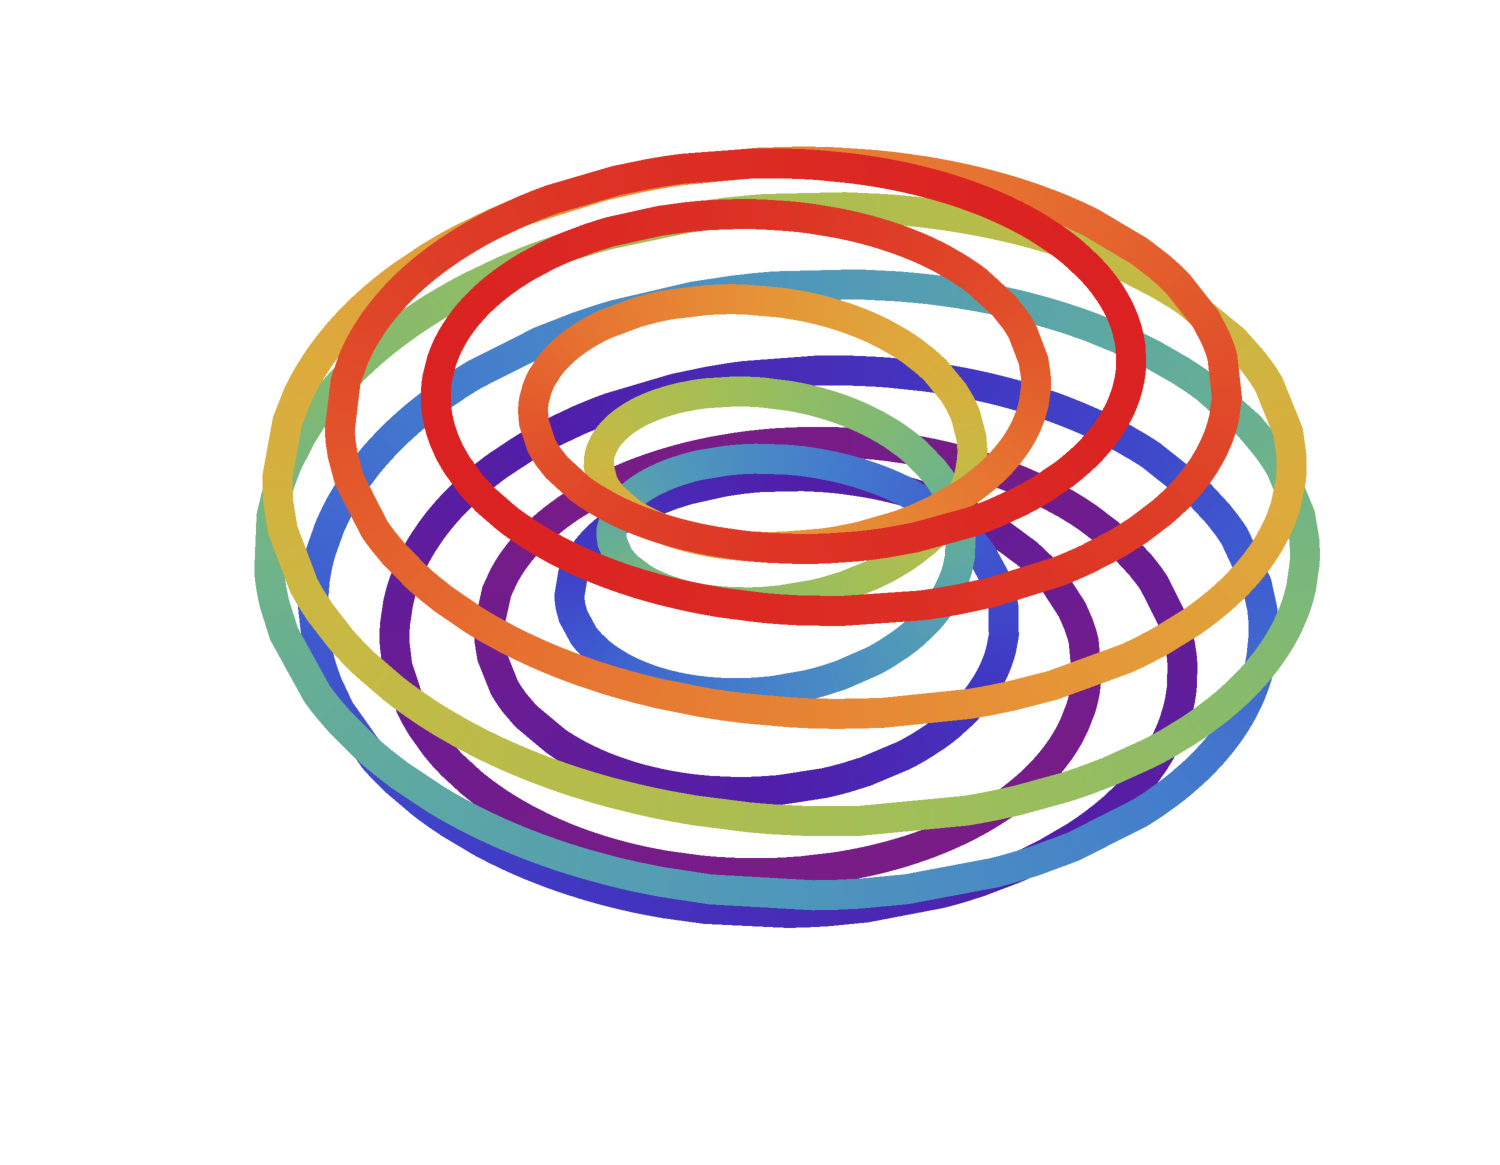
\includegraphics[width=\linewidth]{../data/torus-p11-q2.pdf}
        \subcaption{$p = 11, q = 2$}
    \end{minipage}
\end{figure}

%Węzeł ten leży na torusie $(r - 2)^2 + z^2 = 1$.
% p = 5;
% q = 3;
% ParametricPlot3D[
% {
% Cos [2 Pi p t] (2 + Cos[2 Pi q t]),
% (2 + Cos[2 Pi q t]) Sin[2 Pi p t],
% -Sin[2 Pi q t]},
% {t, 0, 1},
% ColorFunction -> "Rainbow",
% PlotStyle -> Thickness[0.02],
% Boxed -> False,
% Axes -> False
% ]

Okazuje się, że innych obiektów już nie ma.

\begin{proposition}
    Niech $K$ będzie splotem torusowym takim, że żadne z jego ogniw nie jest niewęzłem, czyli postaci $T_{1, 0}$.
    Wtedy dla pewnych całkowitch $p, q$, węzły $K$ oraz $T_{p, q}$ są tego samego typu.
\end{proposition}

\begin{proposition}
    Niech $d$ będzie największym wspólnym dzielnikiem liczb całkowitych $p, q$.
    Wtedy węzeł torusowy $T_{p, q}$ posiada dokładnie $d$ ogniw.
\end{proposition}

Siedem węzłów z tabeli na końcu książki to węzły torusowe.
Są to niewęzeł, $3_1 = T_{3,2}$, $5_1 = T_{5,2}$, $7_1 = T_{7,2}$, $8_{19} = T_{4,3}$, $9_1 = T_{9,2}$ oraz $10_{124} = T_{5, 3}$.

\begin{proposition}
    Niech $p, q$ będą względnie pierwszymi liczbami takimi, że $|p|, |q| \ge 2$.
    Wtedy splot $T_{p, q}$ oraz splot do niego odwrotny, $T_{-p, -q}$, są tego samego typu.
\end{proposition}

Sploty $T_{p, q}$ oraz $T_{q, p}$ również są równoważne.
Murasugi prezentuje w~swojej książce \cite{murasugi96} przyjemny dowód opierający się na następującym lemacie:

\begin{lemma}
    Sfera $S^3$ powstaje z~powierzchni dwóch węzłów trywialnych z~wnętrzem ($D^2 \times S^1$) przez wzajemne sklejenie południka i~równoleżnika z~równoleżnikiem i~południkiem.
\end{lemma}

Przejdźmy do podania wartości różnych niezmienników.

\begin{proposition}
    Niech $L = T_{p, q}$ będzie splotem torusowym o $d$ ogniwach, różnym od $T_{0, 0}$.
\index{wielomian!Alexandera}%
    Wtedy jego wielomianem Alexandera jest
    \begin{equation}
        \alexander_L(t) = (-1)^{d-1} \frac{(1-t)(1 - t^{pq/d})^d}{(1-t^p)(1-t^q)} \cdot t^{-(p-1)(q-1)/2}.
    \end{equation}
\end{proposition}

Przypadek $p = 2$ wymaga prostego rozumowania indukcyjnego.
Samo ćwiczenie pojawia się w~wielu podręcznikach topologii.
Pełny dowód można znaleźć w~\cite[przykład 9.15]{burde14}, gdzie wyznaczono jakobian prezentacji grupy węzła $\langle x, y \mid x^py^{-q}\rangle$.

Inne podejście, formułę Seiferta-Torresa, prezentuje przeglądowa praca Turaewa \cite{turaev86}.
\index{formuła Seiferta-Torresa}

\begin{proof}
    Macierz Seiferta węzła torusowego $L = T_{p, q}$ ma nieskomplikowaną blokową budowę i posłuży nam do znalezienia wielomianu Alexandera wzorem $\alexander = \det (M - tM^t)$.
    % Rachunki są nieco uciążliwe.
    \begin{equation}
        M = \begin{bmatrix}
            B & & & & \\
            -B & B & & & \\
            & \ddots & \ddots & & \\
            & & \ddots & B & \\
            & & & -B & B
        \end{bmatrix},
    \end{equation}
    złożona z~$(q-1)^2$ bloków o~wymiarach $(p-1) \times (p-1)$:
    \begin{equation}
        B = \begin{bmatrix}
            -1 & & & & \\
            1 & -1 & & & \\
            & 1 & \ddots & & \\
            & & \ddots & -1 & \\
            & & & 1 & -1
        \end{bmatrix}.
    \end{equation}
    Rachunki pozostawiamy Czytelnikowi jako ćwiczenie.
\end{proof}

\begin{corollary}
    Niech $K = T_{p, q}$ będzie węzłem torusowym.
    Wtedy jego wielomianem Alexandera jest
    \begin{equation}
         \alexander(t) = \frac{(t^{pq}-1)(t-1)}{(t^p-1)(t^q-1)}.
    \end{equation}
\end{corollary}

\begin{corollary}
    Wielomian Alexandera odróżnia od siebie węzły $(2,n)$-torusowe.
\end{corollary}

\begin{proof}
    Mamy $\alexander(T_{2,n})(t) = (t^n+1) / (t+1)$, więc $\deg \alexander (T_{2,n}) = n - 1$.
\end{proof}

Znajomość wielomianu Alexandera wystarcza na szczęście do podania pełnej klasyfikacji węzłów torusowych bez uciążliwego dowodu.

\begin{proposition}
    Niech $p, q, r, s$ będą liczbami całkowitymi.
    Następujące warunki są równoważne:
    \begin{itemize}
        \item węzły torusowe $T_{q, r}$ oraz $T_{p, s}$ są równoważne,
        \item $\{q, r\} = \{p, s\}$ lub $\{q, r\} = \{-p, -s\}$.
    \end{itemize}
\end{proposition}

\begin{proof}
    Ograniczymy się do przypadku, gdy $p, q, r, s \ge 2$.
    Tylko jedna implikacja wymaga dowodu, w~prawo.
    Bez straty ogólności załóżmy więc, że $q > r$, $p > s$.
    Skoro węzły $T_{q, r}$ i~$T_{p,s}$ są równoważne, to porównanie najwyższych współczynników w~ich wielomianach Alexandera daje równość $(q-1)(r-1) = (p-1)(s-1)$.
    Wymnożenie wszystkiego prowadzi do czterech przypadków: $s = r$, $s = ps$, $qr = r$, $qr = ps$, z~których dwa środkowe nie mogą zachodzić (gdyż $p, q > 1$).
    Z czwartego wynika, że $qr \le s < ps$, czyli sprzeczność.
\end{proof}

Kawauchi pisze, że wcześniej klasyfikacja węzłów torusowych wynikała z klasyfikacji wolnych produktów $(\Z/p) * (\Z/q)$, które są ilorazami grup węzłów torusowych \cite{schreier24}.

Wartości wielomianu Jonesa podajemy bez dowodu:

\begin{proposition}
\index{klamra Kauffmana}%
    Klamra Kauffmana spełnia zależność rekurencyjną
    \begin{equation}
        \bracket{T_{2, n}} = A \bracket{T_{2,n-1}} + (-1)^{n-1} A^{2-3n}
    \end{equation}
    z warunkiem brzegowym $\bracket{T_{2,1}} = -A^3$.
\end{proposition}

\begin{proposition}
\index{wielomian!Jonesa}%
    Niech $L = T_{p, q}$ będzie węzłem torusowym.
    Wtedy jego wielomianem Jonesa jest
    \begin{equation}
        \jones(t) = \frac {{\sqrt t}^{(p-1)(q-1)}}{1-t^2} \cdot (1 - t^{p+1} - t^{q+1} + t^{p+q}).
    \end{equation}
\end{proposition}

Podamy teraz wartości całkowitoliczbowych niezmienników dla węzłów torusowych przy założeniu, że $q$ lub $r$ nie jest zerem.
Nietrywialne węzły torusowe są pierwsze i~odwracalne, ale mają niezerową sygnaturę, więc nie są chiralne.
Wiedział to Schreier w 1924.
% TODO: \cite schreier24?

\begin{proposition}
\index{okres}%
    Węzeł torusowy $T_{p, q}$ ma okres $|p|$ oraz $|q|$.
\end{proposition}

\begin{proposition}
\index{sygnatura}%
    Niech $p, q > 0$ będą liczbami całkowitymi, zaś $R_2$ oznacza resztę z dzielenia przez dwa.
    Zdefiniujmy funkcję $\sigma(p, q) = - \sigma(T_{p, q})$.
    Spełnia zależność rekurencyjną
    \begin{equation}
        \sigma(p, q) = \begin{cases}
             q^2 + \sigma(p-2q, p) - R_2(p)       & \text{jeśli } 2q < p \\
             q^2 - 1                              & \text{jeśli } 2q = p \\
             q^2 - \sigma(2q - p, q) + R_2(r) - 2 & \text{jeśli } 2q > p \ge q
        \end{cases}
    \end{equation}
    z warunkami brzegowymi: $\sigma(p, q) = \sigma(q, p)$, $\sigma(1, q) = 0$, $\sigma(2, q) = q-1$.
\end{proposition}

\begin{proof}
    Dowód zawiera praca \cite{litherland81}.
\end{proof}

Borodzik niedawno przyjrzał się dokładniej sygnaturom węzłów torusowych.
W pracy \cite{borodzik10} napisanej z K. Oleszkiewiczem pokazał, że nie istnieje wymierna funkcja $R(p, q)$, która pokrywałaby się z sygnaturą węzła torusowego $T_{p, q}$ dla wszystkich względnie pierwszych, nieparzystych $p$ oraz $q$.
Uwaga: definicja funkcji $s$ z \cite{borodzik10} zawiera złośliwą literówkę.

\begin{proposition}
    Niech $p, q$ będą względnie pierwszymi liczbami, zaś $C \in [0, 1)$ stałą taką, że $Cpq$ nie jest liczbą całkowitą.
    Przyjmijmy $z = \exp (2 \pi i C)$ i zdefinujmy pomocnicze funkcje: niech $\{x\} = x - \lfloor x \rfloor$ oznacza część ułamkową, zaś
    \begin{equation}
        \langle x \rangle = \begin{cases}
            0 & \text{dla } x \in \Z \\
            \{x\} - 1/2 & \text{dla } x \not \in \Z
        \end{cases}
    \end{equation}
    funkcję piłę.
    Dalej, określmy sumę Dedekinda
    \begin{equation}
        s(p, q, x) = \sum_{j = 0}^{q-1} \left\langle \frac {j}{q} \right\rangle \left\langle \frac {jp}{q} + x \right\rangle.
    \end{equation}
    Przy tych oznaczeniach, sygnatura węzła $(p, q)$-torusowego wyznacza się wzorem
    \begin{align}
        \sigma(z) & = \frac{1}{3pq} \left (p^2 + q^2 + 6 \langle Cpq \rangle^2 - \frac {1}{2} \right)  + 2(C^2 - C) pq + (2-4C) \langle Cpq \rangle + {} \\
        & - 2s(p, q, Cp) - 2s(q, p, Cq) - 2s(p, q, p-pC) - 2s(q, p, q-qC). \nonumber
    \end{align}
\end{proposition}

\begin{corollary}
    Jeśli $p, q$ są nieparzyste i względnie pierwsze, to
    \begin{equation}
        \sigma(T_{p,q}) = \frac{1}{6pq} + \frac{2p}{3q} + \frac{2q}{3p} - \frac{pq}{2} - 4(s(2p, q, 0) + s(2q, p, 0)) - 1.
    \end{equation}
\end{corollary}

\begin{corollary}
    Jeśli $p$ jest nieparzyste, zaś $q > 2$ parzyste, to
    \begin{equation}
        \sigma(T_{p,q}) = - \frac{pq}{2} + 4s(2p, q, 0) - 8s(p, q, 0) + 1.
    \end{equation}
\end{corollary}

\begin{proposition}
\index{indeks skrzyżowaniowy}%
    Mamy $\crossing T_{p, q} = \min \{|pq| - |p|, |pq| - |q|\}$.
\end{proposition}

\begin{proof}
    Murasugi twierdzi, że udowodnił to w \cite{murasugi91}.
\end{proof}

Wyznaczenie indeksu rozwiązującego było dużo trudniejsze.
Murasugi pisze w~książce \cite{murasugi96}, że mamy nierówność
\begin{equation}
    u(T_{p, q}) \le \frac 12 (p-1)(q-1),
\end{equation}
z równością dla względnie pierwszych $p, q > 0$.
Hipoteza Milnora głosiła, że w~rzeczywistości równość zachodzi zawsze.
Dowód został odnaleziony w~latach 1993-1995 przy użyciu tzw. \emph{gauge theory} (działu teorii pola, gdzie lagranżjan jest niezmienniczy względem grup Liego lokalnych transformacji...).

\begin{proposition}
\index{liczba gordyjska}%
\label{prp:torus_unknotting_number}%
    Dla względnie pierwszych $p, q > 0$ mamy
    \begin{equation}
        u(T_{p, q}) = \frac 12 (p - 1)(q - 1),
    \end{equation}
\end{proposition}

% % Rasmussen podał nowy dowód hipotezy Milnora o plastrowym genusie węzłów torusowych, jest to pierwszy dowód który nie zależy od gauge theory.
% https://mathscinet.ams.org/mathscinet-getitem?mr=2729272

\begin{proof}
    Patrz prace \cite{kronheimer93} oraz \cite{kronheimer95}.
    % This last result was proved by F. B. Kronheimer and T. S. Mrowka in [Kronheimer-Mrowka 1993], who determined the 4-dimensional genus of T(p, q) (defined in 12.3) by applying gauge theory to an embedded surface in a 4-manifold.
    % https://web.math.princeton.edu/~petero/GridHomologyBook.pdf strona 4
\end{proof}

Genus pokrywa się z~liczbą gordyjską dla węzłów torusowych, bo wyznacznik macierzy Seiferta jest niezerowy, więc genus to dokładnie stopień wielomianu Alexandera.

Patrz też \cite[s. 149]{murasugi96}.

\begin{proposition}
\index{indeks mostowy}%
\label{prp:torus_bridge_number}%
    $\bridge T_{p, q} = \min \{|p|, |q|\}$
\end{proposition}

Według Murasugiego dowód znajduje się w \cite{schubert54}.

\begin{corollary}
\index{indeks warkoczowy}%
\label{cor:torus_braid_number}%
    Niech $p, q \neq 0$ będą liczbami całkowitymi.
    Wtedy $\braid T_{p, q} = \min \{|p|, |q|\}$.
\end{corollary}

\begin{proof}
    Niech $K$ będzie węzłem torusowym typu $(p,q)$ z~minimalnym przedstawieniem jako warkocz $\beta$.
    Z konstrukcji domknięcia (czyli dołączenia rozłącznych półokręgów) wynika,
    że diagram $K$ ma dokładnie $b(K)$ lokalnych maksimów.
    Definicja indeksu mostowego orzeka, iż $br(K) \le b(K)$.
    Bez straty ogólności niech $p > q > 0$.
    Skoro węzeł $K$ powstaje z~$q$-warkocza $(\sigma_{q-1} \ldots \sigma_2\sigma_1)^p$,
    indeks $b(K)$ nie przekracza $q = br(K)$.
\end{proof}

\begin{proposition}
    Niech $K$ będzie nietrywialnym węzłem, którego grupa ma nietrywialne centrum.
    Wtedy $K$ jest węzłem torusowym.
    % Kawauchi: The torus knots are characterized as the only knots whose groups have non-trivial centers (cf. Corollary 6.3.6).
\end{proposition}

\begin{proof}
    Najpierw pokazali to Murasugi \cite{murasugi61}, Neuwirth \cite{neuwirth61} przy dodatkowym założeniu, że węzeł $K$ jest alternujący,
    wkrótce po tym Burde, Zieschang znaleźli dowód w ogólnym przypadku \cite{burde66}.
\end{proof}

\index{węzeł!torusowy|)}%

% Koniec sekcji Węzły torusowe
\section{Węzły satelitarne} % (fold)

% meridian - południk
% longitude - równoleżnik
Załóżmy, że w dopełnieniu pewnego splotu został zanurzony torus.
Jeżeli jest ściśliwy, to albo równoleżnikl torusa ogranicza dysk w dopełnieniu splotu~i torus jest niezawęźlony, albo południk ogranicza dysk w dopełnieniu splotu i~splot nie przebiega wzdłuż torusa.
Żadna z~tych sytuacji nie jest ciekawa.
Inny zdegenerowany przypadek występuje, gdy torus stanowi rurowe otoczenie jednego z~ogniw splotu.
W przeciwnym razie splot można zbudować z~prostszych obiektów.

Oto formalny opis konstrukcji.
Niech $W$ będzie pełnym torusem.
Dysk zanurzony w $W$, którego brzeg stanowi nieściągalną pętlę w $\partial W$, nazywamy południkowym.
Mówimy, że zamknięta krzywa $\lambda \subseteq W$ jest właściwa, jeżeli przecina wszystkie dyski południkowe.

\begin{definition}[węzeł satelitarny]
    \index{węzeł!satelitarny}
    Niech $P$ będzie splotem zanurzonym w~niezawęźlonym torusie $W$ tak, by co najmniej jedno z~ogniw stanowiło właściwą pętlę w~$W$.
    Niech $C$ będzie węzłem, zaś $V$ jego rurowym otoczeniem.
    Wybierzmy dowolny homeomorfizm $h \colon W \to V$.
    Wtedy splot $S = h(P)$ nazywamy satelitą o~wzorcu $P$ oraz towarzyszu $C$.
\end{definition}

% \begin{definition}
%     Węzeł nazywamy satelitarnym, jeśli zawiera nieściśliwy, nierównoległy do brzegu torus we własnym dopełnieniu.
% \end{definition}

Hoste i inni podejrzewają w~\cite{thistlethwaite98}, że jeśli satelita owija się $m$-krotnie wokół torusa, zaś indeks skrzyżowaniowy towarzysza wynosi $k$, to satelita nie posiada diagramu o~mniej niż $km^2$ skrzyżowaniach.

Ponieważ dla trójlistnika $k = 3$, napotkali się tylko na satelity owijające się $m = 2$ razy podczas tablicowania pierwszych węzłów do 16 skrzyżowań.
Nie spodziewano się żadnego satelity ósemki, gdyż wtedy $k = 4$, zatem każdy satelita miałby co najmniej $4 \cdot 2^2 + 1 = 17$ skrzyżowań: dodatkowe $+1$ jest potrzebne, by nie dostać splotu o~dwóch ogniwach.

Najprostszy satelita ma 13 skrzyżowań.

\begin{example}[swallow-follow torus]
    Klasa węzłów satelitarnych obejmuje węzły złożone.
    W ich przypadku można wskazać pewien szczególny torus nieściśliwy -- połykający pierwszy składnik, a~potem podążający za drugim:\footnote{Źródło: \url{https://mcm-www.jwu.ac.jp/~hayashic/semi/07/07i/07i.html}}
    \begin{figure}[H]
        \centering
        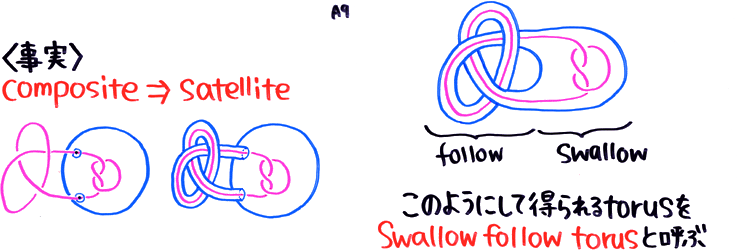
\includegraphics[width=0.75\linewidth]{../data/mixed/follow-swallow.png}
        \caption[something]{Torus połykająco-podążający. Źródło: strona internetowa\footnote{\url{https://mcm-www.jwu.ac.jp/~hayashic/semi/07/07i/07i.html}.} C. Hayashiego.}
    \end{figure}
\end{example}

Schubert pokazał, że zorientowane klasy izotopii węzłów w~$S^3$ tworzą wolny przemienny monoid na przeliczalnie wielu generatorach.
Dowód to uważna analiza nieściśliwych torusów obecnych w~dopełnieniu sumy spójnej.
To doprowadziło go do definicji węzłów satelitarnych i~towarzyszących w~przełomowej pracy \cite{schubert53} oraz zunifikowało teorię 3-rozmaitości z teorią węzłów.
Patrz też \cite{motegi97}.
% czemu akurat Motegi?

Na brzegu torusa $V$ można wprowadzić pewien układ współrzędnych: południk to pętla właściwa w $\partial V$, która ogranicza dysk w $V$, natomiast równoleżnik to pętla w $\partial V$, która spotyka południk raz.
Z~dokładnością do izotopii południk jest jeden, ale równoleżnik nie.
Gdy indeks zaczepienia równoleżnika oraz rdzenia torusa wynosi zero, mówimy, że równoleżnik jest preferowany.

\begin{definition}[dubel Whiteheada]
    \index{dubel Whiteheada}
    Jeżeli $P \subseteq W$ jest skręconym jednokrotnie niewęzłem, to węzeł $S$ nazywamy dublem Whiteheada.
\end{definition}

Każdy węzeł posiada nieskończenie wiele dubli Whiteheada: wystarczy rozciąć torus $V$, skręcić jedną końcówkę i~ponownie zszyć, żaden z~nich nie jest odróżniany od niewęzła przez wielomian Alexandera.

Wyróżnia się pewien szczególny homeomorfizm $h$, który przenosi południk i preferowany równoleżnik $W$ na południk i preferowany równoleżnik $V$.
Nazywamy go wiernym.
% faithful
O dublu względem wiernego homeomorfizmu mówimy, że jest nieskręcony.

\begin{definition}[węzeł kablowy]
    \index{węzeł!kablowy}
    Niech $h \colon W \to V$ będzie wiernym homeomorfizmem, zaś $P$ węzłem $(p, q)$-torusowym.
    Satelitę $S$ nazywamy węzłem $(p, q)$-kablowym albo krótko kablem.
\end{definition}

\begin{proposition}
    Każdy kabel wyznacza jednoznacznie węzeł, z~którego powstał.
\end{proposition}

\begin{proof}
    Wniosek 2 z~pracy \cite{feustel78} Feustela, Whittena pokazuje, że na podstawie kabla można wyznaczyć parametry węzła torusowego $K'_{p,q}$ oraz topologię dopełnienia oryginalnego węzła.
    Wiemy jednak z~twierdzenia Gordona-Lueckego, że różne węzły mają różne dopełnienia.
\end{proof}

Niewęzeł nie ma nietrywialnych węzłów towarzyszących.

\begin{definition}
    Towarzysza $C$ nietrywialnego splotu nazywamy właściwym, jeśli nie jest niewęzłem i~nie jest ogniwem tego splotu.
\end{definition}

Sploty bez właściwych towarzyszy określa się zazwyczaj terminem ,,atoroidalny''.
Patrz też diagram przedstawiony w \cite{cromwell04} na stronie 83.

\begin{proposition}
    Duble nietrywialnych węzłów oraz kable są pierwsze.
\end{proposition}

\begin{proof}
    Jest to wniosek z twierdzenia 4.4.1 w~\cite{cromwell04}: jeśli wzorzec jest niewęzłem lub węzłem pierwszym, to każdy właściwy satelita jest pierwszy.
\end{proof}

Niektóre węzły przedstawiają się jako satelity w~dokładnie jeden sposób, inne nie.
Rok 1979 przyniósł amerykańską pracę \cite{jaco79} oraz niemiecką książkę \cite{johannson79}, gdzie niezależnie od siebie opisano jednoznaczny rozkład, nazywany teraz rozkładem Jaco-Shalena-Johannsona:

\begin{proposition}
    Niech $M$ będzie nierozkładalną, orientowalną, domkniętą 3-rozmaitością.
    Istnieje wtedy jedyna z dokładnością do izotopii minimalna rodzina rozłącnzie zanurzonych nieściśliwych torusów tak, że każda składowa 3-rozmaitości powstałej przez rozcinanie wzdluż torusów jest atoroidalna lub włóknistą przestrzenią Seiferta ($S^1$-wiązką nad dwuwymiarowym orbifoldem).
\end{proposition}

Jest on związany z operacją splatania (ang. \emph{splicing}), będącej uogólnieniem budowania satelitów.
Hipotezę o jedyności rozkładu wysnuł wcześniej Waldhausen.

% Koniec sekcji Węzły satelitarne


\section{Węzły hiperboliczne}
\index{węzeł!hiperboliczny|(}
\label{sec:hyperbolic}
Jak pisaliśmy w~sekcji \ref{sec:mutant}, słynne węzły Conwaya oraz Kinoshity-Terasakiego odróżnił od siebie po raz pierwszy Riley.
\index{węzeł!Conwaya}%
\index{węzeł!Kinoshity-Terasakiego}%
Zbadał paraboliczne reprezentacje ich grup w~skończoną grupę prostą $PSL(2, 7)$, co doprowadziło go do odkrycia struktury hiperbolicznej w~dopełnieniu ósemki \cite{riley75}.
\index{ósemka}
% https://arxiv.org/pdf/2002.00564.pdf
Zainspirowany tym wynikiem Thurston najpierw rozłożył dopełnienie ósemki na dwa idealne wielościany, a~potem znacznie uogólnił swój przykład.

Reszta sekcji powstała na podstawie dwóch źródeł: przeglądowej pracy Kalfagianniego, Futera oraz Purcell \cite{purcell19} i~notatek z~wykładów, które były prowadzone przez samą Purcell.
\index{człowiek!Futer, David}%
\index{człowiek!Kalfagianni, Efstratia}%
\index{człowiek!Purcell, Jessica}%
Wiedzę o~węzłach hiperbolicznych można czerpać także z~artykułu Weeksa \cite{weeks05}.
\index{człowiek!Weeks, Jeff}%

% Badając sploty nie ograniczamy się tylko do diagramów, ale korzystamy też z ich dopełnień, to znaczy 3-rozmaitości $S^3 \setminus L$.
% Jest ona homeomorficzna z wnętrzem zwartej rozmaitości $X(L) = S^3 \setminus N(K)$, zwanej zewnętrzem splotu, gdzie $N(L)$ stanowi rurowe otoczenie splotu.
% Dalej możemy stosować maszynierę topologii 3-rozmaitości.

% \begin{definition}[ściśliwy]
%     Niech orientowalna powierzchnia $S$ będzie właściwie\footnote{properly} zanurzona w zwartej, orientowalnej 3-rozmaitości $M$.
%     Załóżmy, że dla każdego dysku $E \subseteq M$ z brzegiem $\partial E \subseteq S$ istnieje dysk $E' \subseteq S$ taki, że $\partial E = \partial E'$.
%     Mówimy wtedy, że powierzchnia $S$ jest nieściśliwa.
% \end{definition}

% $\partial$-ściśliwość

% essential

% Haken

% monodromy of fibration

% Węzły i sploty, które będziemy rozpatrywać dalej, mają szczególną strukturą geometryczną.

\begin{definition}[hiperboliczny]
    Splot $L$, na dopełnieniu którego można zadać zupełną metrykę o~stałej krzywiźnie $-1$ nazywamy hiperbolicznym.
\end{definition}

\begin{proposition}
    Niech $L$ będzie splotem, zaś $\mathbb H^3$ hiperboliczną 3-przestrzenią.
    Splot $L$ jest hiperboliczny wtedy i~tylko wtedy, gdy $S^3 \setminus L = \mathbb H^3 / \Gamma$, gdzie $\Gamma$ jest dyskretną, beztorsyjną grupą izometrii, izomorficzną z~$\pi_1(S^3 \setminus L)$.
\end{proposition}
% TODO: skąd to jest dokładnie?

Thurston podejrzewał, że każda 3-rozmaitość rozkłada się wzdłuż sfer i~nieściśliwych torusów na części wyposażone w~jedną z~ośmiu kanonicznych geometrii:
\begin{itemize}
\item sferyczną $S^3$, albo euklidesową $E^3$, albo hiperboliczną $H^3$,
\item $S^2 \times \R$, albo $H^2 \times \R$,
\item uniwersalne nakrycie $SL(2, \R)$,
\item geometrię Sol albo geometrię Nil.
\end{itemize}
Nie umiał podać pełnego uzasadnienia, w~pracy \cite{thurston82} udowodnił swoje przypuszczenie dla rozmaitości Hakena.
\index{rozmaitość Hakena}
Dowód hipotezy geometryzacyjnej dostarczył mniej więcej dwie dekady później Perelman, nie to jest jednak dla nas najważniejsze.
\index{hipoteza!geometryzacyjna Thurstona}
Z przełomowych prac Thurstona z~lat 70. oraz 80. wynika coś ciekawszego: że dopełnienie węzła jest rozmaitością włóknistą Seiferta, toroidalną albo hiperboliczną.
Innymi słowy, Thurston przedstawił trychotomię:

\begin{theorem}
    \index{twierdzenie!Thurstona}
    Każdy węzeł jest satelitarny, torusowy albo hiperboliczny.
    \index{węzeł!satelitarny}
    \index{węzeł!torusowy}
\end{theorem}
% luźno związane: http://www.deltami.edu.pl/temat/matematyka/topologia/2012/12/27/%William_Thurston_i_hipoteza_geometryzacyjna/

\begin{proof}
    Thurston w~\cite[wniosek 2.5]{thurston82}.
\end{proof}

% https://mathoverflow.net/a/289359 : hyperbolic, toroidal (that is, satellite), or Seifert fibered

Węzły hiperboliczne stanowią najliczniejszą i~najmniej zrozumianą rodzinę węzłów.
Sam Nead, użytkownik portalu MathOverflow napisał, że kryterium Thurstona dzięki maszynerii JSJ oraz pracom innych osób można wysłowić algebraicznie.

\begin{proposition}
    % There is a topological criterion due to Thurston.  Using the JSJ machine (and work of many others) this criterion can also be phrased algebraically.  I'll essay these below.  Please note that the situation is much simpler for knots.  To answer your question most directly, here is the desired reference to Wikipedia.
    % http://en.wikipedia.org/wiki/Hyperbolic_link
    % This page refers to the books of Colin Adams and William Thurston.  Both are excellent.
    % Now, here is Thurston's criterion. (EDIT: exposition improved after reading Bruno Martelli's answer.)
    % Suppose that $L$ is the link and $X$ is the link complement.  Suppose $\pi = \pi_1(X)$. We assume the following properties (and each property assumes the proceeding ones). $\newcommand{\ZZ}{\mathbb{Z}}$
    %  - $L$ is not a split link.  Equivalently, $X$ is contains no essential two-sphere.  Equivalently, $\pi$ is not a free product.
    %  - $L$ is not the unknot. Equivalently, $X$ contains no essential disk. Equivalently, $\pi$ is not $\ZZ$.
    %  - $L$ has no component that is an "undisturbed satellite knot".  Equivalently, $X$ contains no essential torus.
    %  - $L$ is not a torus knot. Equivalently, $X$ contains no essential annulus. These last two topological properties are equivalent to $\pi$ not containing a copy of $\ZZ^2$.
    % Then $X$ admits a hyperbolic structure.
    Niech $L$ będzie splotem, który nie rozszczepia się, nie jest niewęzłem, nie posiada wśród ogniw niezakłóconego węzła satelitarnego oraz nie jest węzłem torusowym.
    \index{splot!rozszczepialny}
    Wtedy $L$ jest hiperboliczny.
\end{proposition}

\begin{proposition}
    Niech $L$ będzie splotem takim, że jego dopełnienie $S^3 \setminus L$ nie zawiera właściwej 2-sfery, właściwego dysku, właściwego torusa oraz właściwego pierścienia.
    Wtedy $L$ jest hiperboliczny.
\end{proposition}

\begin{proposition}
    Niech $L$ będzie splotem takim, że jego grupa $\pi(S^3 \setminus L)$ nie jest produktem wolnym, nie jest izomorficzna z~$\Z$ oraz nie zawiera w~sobie kopii grupy $\Z \oplus \Z$.
    Wtedy $L$ jest hiperboliczny.
\end{proposition}

\begin{proof}
    Patrz \url{https://mathoverflow.net/a/153327}.
\end{proof}

Czas na podanie jakichś przykładów węzłów hiperbolicznych, za \cite{adams05}.

\begin{proposition}
    Każdy alternujący, pierwszy, oraz nierozszczepialny splot jest albo 2-warkoczem (a zatem, torusowy) albo hiperboliczny.
    \index{węzeł!alternujący}
    \index{węzeł!pierwszy}
    \index{węzeł!rozszczepialny}
\end{proposition}

\begin{proof}
    Menasco \cite{menasco84} pokazał, że dopełnienie alternującego węzła nie zawiera nieściśliwych  nieperyferyjnych torusów.
    To w~połączeniu z~unifikacyjnym twierdzeniem Thurstona dla rozmaitości Hakena kończy dowód.
\index{rozmaitość Hakena}%
    % zarys dowodu zz MathSciNet
\end{proof}

\begin{proposition}
    Nietrywialne pierwsze prawie alternujące węzły są torusowe albo hiperboliczne.
    \index{węzeł!pierwszy}
    \index{węzeł!prawie alternujący}
\end{proposition}

\begin{proof}
    Grupa studentów pod opieką Adamsa w \cite{brock92}.
\end{proof}

\begin{proposition}
    Toroidalnie alternujące węzły pierwsze są torusowe albo hiperboliczne.
    \index{węzeł!pierwszy}
    \index{węzeł!toroidalnie alternujący}
\end{proposition}

Ze wszystkich węzłów pierwszych do 11 skrzyżowań i~pierwszych, nierozszczepialnych splotów do 10 skrzyżowań tylko 3 węzły i~2 sploty nie są toroidalnie alternujące, tak twierdzi Adams \cite{adams05}.

\begin{proof}
    Patrz \cite{adams994}.
\end{proof}

\begin{proposition}
    Sploty Montesinosa są prawie zawsze torusowe albo hiperboliczne.
    \index{splot!Montesinosa}
\end{proposition}

\begin{proof}
    Najpierw zidentyfikowano sploty Montesinosa torusowe, które są też torusowe \cite{boileau80}.
    Potem w~pracy \cite{oertel84} znaleziono listę wyjątków (z chyba trochę inną notacją niż nasza):
    \begin{itemize}
        \item $K(1/2, 1/2, 21/2, 21/2)$,
        \item $K(2/3, 21/3, 21/3)$,
        \item $K(1/2, 21/4, 21/4)$,
        \item $K(1/2, 21/3, 21/6)$,
        \item lub lustra tych splotów. \qedhere
    \end{itemize}
\end{proof}

\begin{proposition}
    Mutant węzła hiperbolicznego jest węzłem hiperbolicznym.
    \index{mutant}
\end{proposition}

\begin{proof}
    Ruberman w~\cite{ruberman87}, patrz wniosek 1.4.
\end{proof}

\begin{proposition}
    Niech $G$ oznacza grupę izometrii wnętrza dopełnienia węzła hiperbolicznego.
    Wtedy $G$ jest diedralna lub skończona cykliczna.
\end{proposition}

\begin{proof}
    Pierwszy był Riley w~artykule \cite[s. 124]{riley79}, można też zapoznać się z~późniejszą pracą \cite{kodama92} Kodamy i Sakumy.
    % Kodama - lemat_1.1
\end{proof}

Kawauchi \cite[s. 131]{kawauchi96} wprowadza jeszcze jedną grupę (grupę symetrii węzła): iloraz grupy PL automorfizmów pary $(S^3, K)$ przez podgrupę elementów, które są otaczająco izotopijne z~odwzorowaniem tożsamościowym.
Okazuje się, że nie wszystkie są skończone:

\begin{proposition}
    Węzeł $K$ ma skończoną grupę symetrii wtedy i~tylko wtedy, gdy jest hiperboliczny, torusowy lub kablem węzła torusowego.
\end{proposition}

Kawauchi nie podaje dowodu, ale zaleca zajrzeć do pracy Sakumy.
Ja zajrzałem i dalej nie mam pojęcia, jak ten dowód miałby wyglądać.

Z kryterium Thurstona mamy prosty wniosek (bo węzły złożone są satelitarne):

\begin{corollary}
    Każdy węzeł hiperboliczny jest pierwszy.
    \index{węzeł!pierwszy}
\end{corollary}

Prawie każdy węzeł pierwszy o~mniej niż 17 skrzyżowaniach jest hiperboliczny, na 32 wyjątki składa się 12 węzłów torusowych oraz 20 satelitów trójlistnika.
Te ostatnie mają co najmniej 13 skrzyżowań.
Baza ciągów liczb całkowitych OEIS zawiera informacje na temat liczności poszczególnych typów węzłów.
Analizując ciągi A051764, A051765 oraz A052408 można dojść do wniosku, że wraz ze wzrostem liczby skrzyżowań, stosunek liczby węzłów hiperbolicznych do wszystkich węzłów dąży do $1$:

\begin{figure}[H]
\renewcommand*{\arraystretch}{1.4}
\footnotesize
\begin{longtable}{lcccccccccccccc}
\hline
    \textbf{rodzaj} & 3 & 4 & 5 & 6 & 7 & 8  & 9  & 10  & 11  & 12   & 13   & 14    & 15     \\ \hline \endhead
    torusowe        & 1 & 0 & 1 & 0 & 1 & 1  & 1  & 1   & 1   & 0    & 1    & 1     & 2      \\
    satelitarne     & 0 & 0 & 0 & 0 & 0 & 0  & 0  & 0   & 0   & 0    & 2    & 2     & 6      \\
    hiperboliczne   & 0 & 1 & 1 & 3 & 6 & 20 & 48 & 164 & 551 & 2176 & 9985 & 46969 & 253285 \\
    \hline
\end{longtable}
\normalsize
\end{figure}

W pracy \cite{malyutin16} Malutin pokazał jednak, że to przypuszczenie jest sprzeczne z~wieloma innymi starymi hipotezami teorii węzłów: \ref{con:malyutin1} -- \ref{con:malyutin4}.

\begin{conjecture}
    \label{con:malyutin1}
    Indeks skrzyżowaniowy jest addytywny względem sumy spójnej.
    \index{indeks skrzyżowaniowy}
    \index{suma spójna}
\end{conjecture}

(To jest powtórzenie hipotezy \ref{con:crossing_additive}).

\begin{conjecture}
    Satelita ma większy (w słabszej wersji: nie mniejszy) indeks skrzyżowaniowy niż jego towarzysze.
    \index{węzeł!satelitarny}
\end{conjecture}

Lackenby pokazał w~\cite{lackenby14}, że jeśli $K$ jest satelitą z~towarzyszem $L$, to $\crossing K \ge 10^{-13} \crossing L$.

\begin{conjecture}
%label{con:malyutin3}
    Węzeł złożony ma większy (w słabszej wersji: nie mniejszy) indeks skrzyżowaniowy niż jego składniki.
    \index{węzeł!pierwszy}
\end{conjecture}

Mówimy, że węzeł pierwszy $P$ jest $\lambda$-regularny, jeśli $\crossing K \ge \lambda \cdot \crossing P$ za każdym razem, gdy węzeł $P$ jest składnikiem węzła $K$.
\index{węzeł!regularny}
Zatem hipotezę można wysłowić krótko ,,węzły pierwsze są $1$-regularne''.
Z tego, co pisaliśmy po hipotezie \ref{con:crossing_additive} wynika, że hipoteza \ref{con:malyutin1} jest prawdziwa w~klasie węzłów alternujących czy torusowych i~że wszystkie węzły są $1/152$-regularne.
% diao04 -> tw. 3.8

\begin{conjecture}
    \label{con:malyutin4}
    Węzły pierwsze są $2/3$-regularne.
\end{conjecture}

Rozwiązanie zagadki przyniosła praca samego Malutina \cite{malyutin19} opublikowana latem 2019 roku, przynajmniej dla splotów.
Pokazał w~niej, że jeśli oznaczymy liczbę splotów pierwszych i~nierozszczepialnych o~$n$ lub mniej skrzyżowaniach przez $P_n$, zaś liczbę hiperbolicznych splotów, także o~$n$ lub mniej skrzyżowaniach, przez $H_n$, prawdziwe będzie oszacowanie
\index{splot!rozszczepialny}
\index{węzeł!pierwszy}
\begin{equation}
    \liminf_{n \to \infty} \frac{H_n}{P_n} < 1 - 10^{-13}.
\end{equation}

Czwarty rozdział książki \cite{purcell20} zawiera ćwiczenie, by znaleźć dwuparametrową rodzinę zupełnych struktur hiperbolicznych na dziurawym torusie oraz czterokrotnie dziurawej sferze.
Elastyczność tego rodzaju nie występuje w~przestrzeniach wyższych wymiarów.
Z~twierdzenia o~sztywności, w~wersji algebraicznej:

\begin{theorem}[Mostow-Prasad]
    \index{twierdzenie!o sztywności}
    Niech $\Gamma_1, \Gamma_2$ będą dyskretnymi podgrupami grupy izometrii $\mathbb H^n$ dla $n \ge 3$ takimi, że ilorazy $\mathbb H^n/\Gamma_i$ mają skończone objętości.
    Załóżmy też, że istnieje izomorfizm grup $\varphi \colon \Gamma_1 \to \Gamma_2$.
    Wtedy podgrupy $\Gamma_1, \Gamma_2$ są sprzężone.
\end{theorem}
\index{twierdzenie!Mostowa-Prasada}

albo geometrycznej:

\begin{theorem}[Mostow-Prasad]
    Niech $M_1, M_2$ będą zupełnymi, hiperbolicznymi rozmaitościami o skończonych objętościach.
    Wtedy każdy izomorfizm grup podstawowych $\varphi \colon \pi_1(M_1) \to \pi_1(M_2)$ realizowany jest jednoznacznie przez izometrię.
\end{theorem}

wynika, że jeśli znaleźliśmy jakąś zupełną strukturę hiperboliczną na dopełnieniu splotu, to innych już nie ma.

\begin{proof}
    Thurston przedstawił szkic rozumowania w~sekcji 5.9 swoich notatek, na bazie których powstała później książka \cite{thurston97}.
    Inne szczegółowe rozumowanie można znaleźć w~rozdziale C podręcznika Benedettiego, Petronio \cite{benedetti92}.
    Patrz także oryginalne prace: Mostowa \cite{mostow73}, Prasada \cite{prasad73}.
\end{proof}

Twierdzenie Mostowa-Prasada pozwala nam na wprowadzenie nowych niezmienników splotów hiperbolicznych: wystarczy wziąć dowolny geometryczny niezmiennik dopełnienia węzła.
Najważniejszym z~nich wydaje się być objętość.

\index{objętość|(}
\begin{definition}[objętość]
    Niech $L$ będzie splotem hiperbolicznym.
    Objętość dopełnienia $L$ względem zupełnej metryki hiperbolicznej nazywamy objętością splotu $L$ i~oznaczamy $\volume L$.
\end{definition}

Objętość jest zawsze skończoną liczbą rzeczywistą.
Dla wygody przyjmuje się czasami, że objętość węzłów torusowych oraz satelitarnych wynosi $0$.
Komputerowy program SnapPea napisany przez Weeksa pozwala na wyznaczenie objętości dowolnego splotu o~rozsądnej ilości skrzyżowań.
\index{SnapPea}

\begin{example}
    $\volume 4_1 = -6 \int_{0}^{\pi/3} \log |2\sin \theta| \,\mathrm{d}\theta \approx 2.0298832$.
\end{example}

Patrz też ciąg A091518 w~bazie danych OEIS.
Jak zobaczymy później, żaden węzeł nie ma mniejszej objętości.

\begin{example}
    $\volume 5_2 \approx 2.82812$.
\end{example}

W encyklopedii Wolfram Mathworld znajduje się informacja, że $5_2$ oraz pewien węzeł o~dwunastu skrzyżowaniach mają tę samą objętość, prawdopodobnie chodzi tu o~$12n_{242}$, który znany jest także jako $(-2, 3, 7)$-precel.
\index{precel!(-2, 3, 7)}

\begin{example}
    $\volume 6_1 \approx 3.16396$.
\end{example}

\begin{example}
    $\volume 6_2 \approx 4.40083$.
\end{example}

\begin{example}
    $\volume 6_3 \approx 5.69302$.
\end{example}

\begin{example}
    $\volume 7_4 \approx 5.13794$.
\end{example}

\begin{example}
    Niech $K$ będzie jednym z~dwóch węzłów w~parze Perko.
    Wtedy $\volume K \approx 5.63877$.
    \index{para Perko}
\end{example}

Praca \cite{purcell19} wspomina kilka przyjemnych ograniczeń, jakie musi spełniać objętość.
Aby je przytoczyć, musimy najpierw zdefiniować dwie stałe: $v_4$ oraz $v_8$, odpowiednio objętość idealnego czworościanu\footnote{Albo rozmaitości Giesekinga, powstałej z czworościanu przez usunięcie  wierzchołków i sklejenie ściany 012 z 310 oraz 023 z 321. Dopełnienie ósemki jest podwójnym nakryciem tej rozmaitości.\index{rozmaitość Giesekinga}} oraz ośmiościanu foremnego w~$\mathbb H^3$.
Mamy
\begin{align}
    v_4 & = \int_{0}^{2\pi/3} \log(2 \cos(\theta/2)) \,\mathrm{d}\theta \approx 1.01494\,16064, \\
    % https://en.wikipedia.org/wiki/Gieseking_manifold
    v_8 & = 4 \sum_{n=0}^\infty \frac{(-1)^n}{(2n+1)^2} \approx 3.66386\,23767. % ... 08876060218414059729536443096597497126688537065 ... \ldots
\end{align}

I tak najpierw Adams pokazał w~swojej rozprawie doktorskiej \cite{adams83}:

\begin{proposition}
    Niech $D$ będzie diagramem hiperbolicznego splotu o~$\crossing L \ge 5$ skrzyżowaniach.
    Wtedy
    \begin{equation}
        \volume L \le 4 (\crossing D - 4) v_4.
    \end{equation}
\end{proposition}

A trzy dekady później poprawił wswój wynik w~\cite{adams13}:

\begin{proposition}
    Niech $D$ będzie diagramem hiperbolicznego splotu o~$\crossing L \ge 5$ skrzyżowaniach.
    Wtedy
    \begin{equation}
        \volume L \le (\crossing D - 5) v_8 + 4v_4.
    \end{equation}
\end{proposition}

Jego metoda polega na podzieleniu dopełnienia splotu na czterościany i~ośmiościany oraz policzeniu ich.
To, w~połączeniu ze znanymi ograniczeniami na objętość ,,cegiełek'', wystarcza.
Podział na ośmiościany zaproponował Dylan (nie William!) Thurston.
% wiem to z purcell19

Thurston zauważył \cite[s. 365]{thurston82}, że tylko skończenie wiele hiperbolicznych 3-rozmaitości może mieć tę samą objętość -- wynika to z~prac Gromowa i~Jørgensena.
Następnie Wielenberg przedstawił w~\cite{wielenberg81} przykłady pokazujące, że istnieją dowolnie duże kolizje wśród węzłów hiperbolicznych: pewne podgrupy klasycznej grupy Picarda działają jako izometrie na górną półprzestrzestrzeń hiperboliczną wymiaru 3 mają podstawowe wielościany, które są takie same jako zbiory, ale różnią się jeśli chodzi o~utożsamienie ze sobą ścian.

Chociaż mutanty mają tę samą objętość hiperboliczną (fakt \ref{mutants_the_same_volume}), to praktyka pokazuje, że ten niezmiennik dobrze wspomaga proces tablicowania węzłów.

\begin{proposition}
    Zbiór
    \[
        \{\volume K: K \textrm{ jest hiperboliczny}\} \subseteq \R
    \]
    jest dobrze uporządkowany, typu porządkowego $\omega^\omega$.
\end{proposition}

\begin{proof}[Niedowód]
    Zdaniem angielskiej Wikipedii, dowód jest gdzieś w~\cite{neumann85} (gdzie Neumann znajduje eleganckie oszacowanie zmiany objętości po wykonaniu chirurgii Dehna), ja tego nie widzę.
    %=% wikipedia - angielski artykuł "hyperbolic volume" 
    Hodgson, Masa \cite{hodgson13} sugerują, że dowód da się znaleźć w notatkach Thurstona \cite{thurston02}.
\end{proof}

W dowolnej rodzinie węzłów istnieje element o~najmniejszej objętości.
Przytoczę teraz przykłady konkretnych rodzin i najmniejszych węzłów, za \cite[s. 16-17]{purcell19} oraz \cite[s. 1-99]{hodgson13}.

\begin{proposition}
%label{prp:eight_least_hyperbolic}
    Żaden węzeł nie ma mniejszej objętości hiperbolicznej od ósemki.
    \index{ósemka}
\end{proposition}

\begin{proof}
    Cao, Meyerhoff w~\cite{cao01} przeanalizowali pakowania horokul w~uniwersalnym nakryciu związanym z~rozmaitościami.
    Doszli do wniosku, że nie ma tam dostatecznieo wolnego miejsca, jeżeli szpic (cusp) nie jest odpowiedniego rozmiaru.
    Trzykrotnie wspierają się przy tym pomocą komputera, by sprawdzić, że określone warunki są spełnione we wszystkich punktach danej przestrzeni parametrów.
\end{proof}

\begin{proposition}
% DICTIONARY;cusped;szpiczasta;rozmaitość
% DICTIONARY;manifold;rozmaitość;-
\index{splot!Whiteheada}%
\index{ósemka}%
    Wśród orientowalnych 3-rozmaitości ze szpicem\footnote{rozmaitość szpiczasta -- niezwarte, zupełne hiperboliczne rozmaitości ze skończoną objętością Riemanna} najmniejszą objętość posiada dopełnienie ósemki oraz jego bliźniak, otrzymany przez $(5, 1)$-chirurgię jednego z~ogniw splotu Whiteheada.
% sformułowanie wygląda jak z "THE MINIMAL VOLUME ORIENTABLE HYPERBOLIC 3-MANIFOLD WITH 4 CUSPS"
\end{proposition}

Klasa rozmaitości wspomniana w fakcie obejmuje dopełnienia hiperbolicznych węzłów.
Powyższy fakt także został wzięty z~pracy \cite{cao01}.

Meyerhoff nie przestawał pracować nad rozmaitościami o~małych objętościach i~osiem lat później w~\cite{meyerhoff09} przedstawił z Gabaiem, Milleyem bez dowodu (obiecali pokazać go później):

\begin{proposition}
    Istnieje 10 orientowalnych 3-rozmaitości z~jednym szpicem o~objętości co najwyżej $2.848$: \texttt{m003}, \texttt{m004} ($\approx 2.02988$), \texttt{m006}, \texttt{m007} ($\approx 2.56897$), \texttt{m009}, \texttt{m010} ($\approx 2.66674$), \texttt{m011} ($\approx 2.78183$), \texttt{m015}, \texttt{m016} oraz \texttt{m017} ($\approx 2.82812$).
    Nazwy pochodzą ze spisu rozmaitości programu SnapPy.
\end{proposition}

Udało mi się rozszyfrować niektóre nazwy.
\texttt{m003} to siostra $4_1$, % https://hal.archives-ouvertes.fr/hal-02867890/document Michel Planat - Quantum computing thanks to Bianchi groups
\texttt{m004} to węzeł $4_1$, % SnapPy - also known as
% m006
% m007
% m009
% m010
% m011
\texttt{m015} to węzeł $5_2$,
\texttt{m016} to węzeł $12n242$, czyli znany nam już $(-2, 3, 7)$-precel,
\index{precel!(-2, 3, 7)}%
\texttt{m017} to siostra $5_2$. % https://arxiv.org/pdf/2107.03275.pdf

W tej samej pracy możemy jeszcze znaleźć informację, że:

\begin{proposition}
    Istnieje dokładnie jedna domknięta hiperboliczna 3-rozmaitość o najmniejszej objętości, rozmaitość Weeksa.
\end{proposition}

Rozmaitość Weeksa została odkryta przez Jeffreya Weeksa w jego rozprawie doktorskiej (1985) oraz niezależnie przez Matwiejewa, Fomenko (1988).
\index{rozmaitość Weeksa}
Powstaje ona przez wykonanie $(5, 2)$ oraz $(5, 1)$ chirurgii Dehna na dopełnieniu splotu Whiteheada, zaś jej objętość wynosi w~przybliżeniu $0.94270$. % https://oeis.org/A126774
\index{splot!Whiteheada}

Następna jest rozmaitość Meyerhoffa, powstała po $(5, 1)$ chirurgii na dopełnieniu ósemki.
\index{rozmaitość Meyerhoffa}
Meyerhoff sugerował w 1987, że ma najmniejszą objętość, ale okazało się potem, że ta wynosi $\approx 0.98136$.

\begin{proposition}
    Wśród orientowalnych 3-rozmaitości o~dwóch szpicach najmniejszą objętość mają splot Whiteheada oraz $(-2, 3, 8)$-precel.
\index{splot!Whiteheada}%
\index{precel!(-2, 3, 8)}%
\end{proposition}

% TODO: check cusped manifold in dictionary

Ich objętość wynosi $v_8$.

\begin{proof}
    Agol \cite{agol10} korzystając z metod topologicznych dowodzi istnienia ,,niezbędnej'' (z ang. essential) powierzchni, która zadaje dolne ograniczenie na objętość i skutecznie krępuje rozmaitości, które mogą to ograniczenie zrealizować.
\end{proof}

Przypadek trzech szpiców nie jest zbyt dobrze zrozumiany.

\begin{proposition}
    Wśród orientowalnych 3-rozmaitości o~czterech szpicach najmniejszą objętość posiada dopełnienie splotu $8_4^2$ wg numeracji Rolfsena (L8a13).
\end{proposition}

\begin{proof}
    Rozumowanie Yoshidy \cite{yoshida13} oparte o pracę Agola.
    Objętość splotu wynosi $2v_8$.
\end{proof}

\index{objętość|)}

\index{węzeł!hiperboliczny|)}

% Koniec sekcji Węzły hiperboliczne



\section{Węzły plastrowe i taśmowe}
\label{sec:slice}
Węzły plastrowe i taśmowe oraz pojęcie kobordyzmu, które wkrótce opiszemy, należą do świata 4-wymiarowej teorii węzłów.
Nie zapoznamy się z nią bliżej oraz nie podamy naszego ulubionego odniesienia do tego tematu w~literaturze, ponieważ sami nie rozumiemy go zbyt dobrze.
Wszystko zaczęło się od artykułu \cite{fox66} Foxa, Milnora.

%%% Kawauchi 155:

\begin{definition}[płaski dysk]
    Niech $D \subseteq B^4$ będzie dyskiem posiadającym otoczenie $N$, kopię zbioru $D \times I^2$, która przecina sferę $S^3$ dokładnie w $\partial D \times I^2$.
    Mówimy wtedy, że dysk $D$ jest płaski.
\end{definition}

\begin{tobedone}
    Płaski? Lokalnie płaski?
    \cite[s. 155]{kawauchi96}
\end{tobedone}

\begin{definition}[węzeł plastrowy]
    \index{węzeł!plastrowy}
    % z \cite{gompf86}
    Niech $K$ będzie takim węzłem w $S^3 = \partial B^4$, który ogranicza gładko zanurzony 2-dysk w $B^4$.
    O węźle $K$ mówimy wtedy, że jest plastrowy.
    % stare:
    % Niech $K \subseteq S^3$ będzie takim węzłem, że w kuli $B^4$ istnieje płaski dysk $D$ taki, że $K = \partial D = D \cap S^3$.
    % Wtedy $K$ nazywamy węzłem plastrowym.
\end{definition}

Następujące węzły o~mniej niż jedenastu skrzyżowaniach są plastrowe: $6_1$, $8_{8}$, $8_{9}$, $8_{20}$, $9_{27}$, $9_{41}$, $9_{46}$, $10_{3}$, $10_{22}$, $10_{35}$, $10_{42}$, $10_{48}$, $10_{75}$, $10_{87}$, $10_{99}$, $10_{123}$, $10_{129}$, $10_{137}$, $10_{140}$, $10_{153}$ oraz $10_{155}$.
\index{węzeł!Conwaya}
Wśród pierwszych węzłów do dwunastu skrzyżowań najdłużej opierał się węzeł Conwaya, aż Piccirillo pokazała w~\cite{piccirillo20}, że nie jest plastrowy.
\index[persons]{Piccirillo, Lisa}%

\begin{proposition}
    Niech $K$ będzie węzłem.
    Wtedy $K \shrap mr K$ jest węzłem plastrowym.
\end{proposition}

\begin{proof}[Niedowód]
\index[persons]{Fox, Ralph}%
\index[persons]{Milnor, John}%
    Pierwszy był Fox z Milnorem \cite{fox66}, patrz także lemat 12.1.2.2 w \cite{kawauchi96}.
\end{proof}

\begin{proposition}
    Albo wszystkie trzy węzły $K_1, K_2, K_1 \shrap K_2$ są plastrowe, albo co najwyżej jeden z~nich.
\end{proposition}

\begin{proof}[Niedowód]
    Lemat 12.1.2.3 w \cite{kawauchi96}.
\end{proof}

Pierwszym poważnym wynikiem z dziedziny teorii węzłów plastrowych, pochodzącym jeszcze z pracy \cite{fox66}, był:

\begin{proposition}[warunek Foxa-Milnora]
    \index{warunek!Foxa-Milnora}
    Niech $K$ będzie węzłem plastrowym.
    Wtedy jego wielomian Alexandera jest postaci $\alexander(t) = f(t) f(1/t)$ dla pewnego wielomianu Laurenta $f \in \Z[t, 1/t]$.
\end{proposition}

\begin{corollary}
    \index{wyznacznik}
    Wyznacznik węzła plastrowego jest kwadratem.
\end{corollary}

\begin{proof}
    Mamy $\det K = |\alexander(-1)| = f(-1) f(-1)$.
\end{proof}

Ten prosty test stwierdza, że 2743 spośród 2977 węzłów o mniej niż 13 skrzyżowaniach nie jest plastrowych.

\begin{proposition}
    \index{sygnatura}
%label{prp:slice_signature}
    Niech $K$ będzie węzłem plastrowym.
    Wtedy $\sigma(K) = 0$.
\end{proposition}

\begin{tobedone}[Szkic dowodu]
    Ustalmy odwzorowanie $f$, które jest nieosobliwe, symetryczne i~dwuliniowe, z~przestrzeni $V$ o~wymiarze $2n$ oraz wyznaczoną przez nie formę kwadratową.
    Jeśli znika ona na podprzestrzeni wymiaru $n$, to ma zerową sygnaturę.
    dowód znaleziony w~podręczniku Lickorisha.
    Patrz też twierdzenie 8.8 z~artykułu \cite{murasugi65}.
    Praca "Infinite Order Amphicheiral Knots". (Charles Livingston, 2001) -- chyba nie?
\end{tobedone}

Test ten eliminuje kolejne 45 węzłów poniżej 13 skrzyżowań.

\begin{proposition}
    \index{niezmiennik!Arfa}
    Niech $K$ będzie węzłem plastrowym.
    Wtedy $\operatorname{Arf} K = 0$.
\end{proposition}

\begin{proof}
    Ustalmy węzeł $K$, wiemy już, że jego wyznacznik jest kwadratem, a na mocy faktu \ref{cor:knot_determinant_odd} także tyle, że jest liczbą nieparzystą.
    Wynika stąd przystawanie $\det K \equiv 1 \mod 8$, które w~połączeniu z warunkiem Murasugiego (fakt \ref{prp:arf_murasugi}) daje $\operatorname{Arf} K = 0$.
\end{proof}

\begin{proposition}
    \label{prp:trivial_alexander_implies_slice}
    Niech $K$ będzie węzłem w kategorii TOP.
    Jeżeli jego wielomian Alexandera jest trywialny: $\alexander_K(t) \equiv 1$, to węzeł $K$ jest plastrowy.
\end{proposition}

\begin{proof}
\index[persons]{Freedman, Michael}%
    Freedman w \cite[tw. 1.13]{freedman82}.
\end{proof}

Implikacja \ref{prp:trivial_alexander_implies_slice} przestaje być prawdziwa po przejściu do kategorii PL.
Dość klarownie różnicę między kategoriami TOP i PL tłumaczy Gompf w~\cite{gompf86}, wspomniane jest tam także twierdzenie Donaldsona, kluczowy składnik w~uzasadnieniu tej różnicy.
\index[persons]{Gompf, Robert}%


%%% Kawauchi 156:
\subsection{Zgodność}
Zgodność jest relacją równoważności na zbiorze węzłów, która prowadzi do nowej definicji węzłów plastrowych (patrz fakt~\ref{prp:concordant_iff_sum_slice}).
My przytaczamy jej definicję z pracy Gompfa \cite{gompf86}:

\begin{definition}[zgodność]
\index{zgodność}%
\index{węzeł!zgodny|see {zgodność}}%
    Dwa węzły $K_0, K_1$ nazywamy (gładko) zgodnymi, jeżeli istnieje gładko zanurzony pierścień w $S^3 \times I$, którego brzegiem jest zbiór $K_0 \times \{0\} \cup K_1 \times \{1\}$.
\end{definition}

Kawauchi \cite[s. 156]{kawauchi96} pisze ,,Two knots (…) are knot cobordant (or concordant)'', więc tak jak wielu innych autorów nie odróżnia więc węzłów kobordantnych od zgodnych.
Mamy zamiar zrobić dokładnie to samo: różnica między tymi terminami jest subtelna; węzły zgodne są też kobordantne, ale implikacja w drugą stronę nie zachodzi (wiemy o~tym z~tekstu Blanlœila ,,Cobordism and Concordance of Knots'') chyba, że pracuje się z węzłami sferycznmi, a tak jest w klasycznej teorii węzłów.
\index[persons]{Blanloeil, Vincent}%
% https://www.maths.ed.ac.uk/~v1ranick/papers/blanloeil
% Concordant knots are cobordant, but the converse is not true in general.
% "Cobordism and Concordance of Knots" by Vincent Blanlœil

Dlatego my będziemy zawsze pisać o węzłach zgodnych i nigdy o kobordantnynch.

\begin{proposition}
\label{prp:concordant_iff_sum_slice}%
    Dwa węzły $K_1, K_2$ są zgodne wtedy i tylko wtedy, gdy suma $(mr K_0) \shrap K_1$ jest plastrowa.
\end{proposition}

\begin{proof}
    Ćwiczenie 12.1.3 w książce Kawauchiego \cite{kawauchi96}.
\end{proof}

\begin{definition}
    Węzeł zgodny z~niewęzłem nazywamy plastrowym.
\end{definition}

,,Bycie zgodnym'' jest relacją równoważności, słabszą od ,,bycia izotopijnym'', ale chyba mocniejszą od ,,bycia homotopijnym''.
% ale mocniejszą od homotopii?
% izotopia: https://encyclopediaofmath.org/wiki/Cobordism_of_knots
% homotopia: https://en.wikipedia.org/wiki/Link_concordance By its nature, link concordance is an equivalence relation. It is weaker than isotopy, and stronger than homotopy: isotopy implies concordance implies homotopy. A link is a slice link if it is concordant to the unlink.
Klasę abstrakcji węzła $K$ oznaczamy przez $[K]$.

\begin{definition}[grupa zgodności]
\index{grupa!zgodności}%
    Niech $C^1$ oznacza iloraz zbioru wszystkich węzłów przez relację zgodności.
    Zbiór $C^1$ wyposażony w~działanie
    \begin{equation}
        [K_1] + [K_2] = [K_1 \shrap K_2]
    \end{equation}
    staje się grupą abelową, nazywaną grupą zgodności.
    Jej elementem neutralnym jest klasa abstrakcji niewęzła.
    Elementem przeciwnym do $[K]$ jest $[mr K]$.
\end{definition}

%%% Kawauchi 157:

Niech $\Theta$ oznacza rodzinę macierzy Seiferta węzłów (czyli kwadratowych macierzy $V$ o~całkowitych wyrazach takich, że $\det (V - V^T) = 1$).
Mówimy, że macierz $V \in \Theta$ jest zerowo kobordantna, jeżeli jest postaci
\begin{equation}
    V = P \begin{pmatrix} 0 & V_{21} \\ V_{12} & V_{22} \end{pmatrix} P^{-1}
\end{equation}
dla pewnej całkowitoliczbowej macierzy $P$ o~wyznaczniku $\pm 1$; takie macierze nazywamy unimodularnie sprzężonymi.
\index{macierz!unimodularnie sprzężona}%
Każda zerowo kobordantna macierz $V \in \Theta$ stanowi macierz Seiferta pewnego plastrowego węzła $K$.
Kawauchi nazywa te węzły algebraicznie plastrowymi i~mówi, że to dokładnie węzły, które ograniczają izotropowe powierzchnie w kuli $B^4$, więc każdy węzeł plastrowy jest algebraicznie plastrowy.

Suma $(-V) \oplus V$ jest zerowo kobordantna dla każdej macierzy $V \in \Theta$.
To (chyba to) inspiruje Kawauchiego do wprowadzenia kolejnej definicji: dwie macierze $V_1, V_2 \in \Theta$ nazywa kobordantnymi, jeżeli $(-V_1) \oplus V_2$ jest zerowo kobordantna.
Kobordyzm stanowi relację równoważności na $\Theta$ -- iloraz $\Theta$ przez tę relację oznacza się $G_-$, jest grupą abelową.

\begin{proposition}
    % Kawauchi 12.2.8
    Odwzorowanie $\psi \colon C^1 \to G_-$ posyłające klasę abstrakcji węzła w klasę abstrakcji jego macierzy Seiferta jest dobrze określonym epimorfizmem.
\end{proposition}

\begin{proof}
    Nie umiem nic sam udowodnić, więc wymienię tylko trzy odsyłacze: z faktu~\ref{prp:cobordant_to_algebraic_is_algebraic} wynika, że odwzorowanie $\psi$ jest dobrze określone, dowód faktu~\ref{prp:signature_additive} pokazuje, że $\psi$ jest homomorfizmem, zaś w \cite[s. 62]{kawauchi96} można przeczytać, dlaczego jest ,,na''.
\end{proof}

Funkcję $\psi$ rozpatrywał Levine \cite{levine69} w latach sześćdziesiątych.
\index[persons]{Levine, Jerome}%
Po mniej niż dekadzie Casson, Gordon \cite{gordon78} wskazali nietrywialne elementy jądra.
\index[persons]{Gordon, Cameron}%
\index[persons]{Casson, Andrew}%
% to wyżej wiem z kawauchi98, "Supplementary notes for Chapter 12"
Potem był wynik Jianga \cite{jiang81}, że jądro nie jest skończenie generowalne, bo zawiera izomorficzną kopię $\Z^\infty$, a~jeszcze później Livingstona \cite{livingston99}, że zawiera też kopię $(\Z/2\Z)^\infty$.
% to wyżej wiem z https://mathscinet.ams.org/mathscinet-getitem?mr=2179265, pierwsze strony tekstu (nie recenzji)

\begin{proposition}
    $G_- \cong \Z^\infty \oplus (\Z/4\Z)^\infty \oplus (\Z/2\Z)^\infty$.
\end{proposition}

Kawauchi \cite[s. 161]{kawauchi96} bez uzasadnienia postanawia nie przytoczyć dowodu tego faktu, ale opowiada krótko, jaka jest idea przewodnia i odsyła wprost do pracy Levine'a.
Na dalszych stronach jego pracy przeglądowej pojawiają się jakieś formy kwadratowe oraz uogólnienia wszystkiego do zgodności splotów, ale ja wracam nocnym pociągiem, więc nie mam siły o tym pisać.




\subsection{Węzły taśmowe}
\index{węzeł!taśmowy|(}%
\begin{definition}
    Węzeł $K = f(S^1)$ będący brzegiem osobliwego dysku $f \colon D \to S^3$ posiadającego następującą własność: każda przecinająca siebie składowa jest łukiem $A \subseteq f(D^2)$, dla którego $f^{-1}(A)$ składa się z~dwóch łuków w~$D^2$ (jeden z~nich jest wewnętrzny), nazywamy taśmowym.
\end{definition}

Jak pisze Kawauchi, mamy oczywiste wynikanie:

\begin{proposition}
\index{węzeł!plastrowy}%
    Każdy węzeł taśmowy jest plastrowy.
\end{proposition}

Dawno temu Fox \cite[problem 1.33]{kirby78} zapytał, czy implikacja odwrotna jest prawdziwa:
\index[persons]{Fox, Ralph}%

\begin{conjecture}[slice-ribbon problem]
    \index{hipoteza!plastrowo-taśmowa}
    Czy każdy węzeł plastrowy jest taśmowy?
\end{conjecture}

Wprawdzie Lisca pokazał prawdziwość hipotezy dla węzłów dwumostowych \cite{lisca07},
\index[persons]{Lisca, Paolo}%
% korzystając ze słynnego tw. Donaldsona: that a definite intersection form of a compact, oriented, simply connected, smooth manifold of dimension 4 is diagonalisable
\index{węzeł!dwumostowy}%
zaś Greene oraz Jabuka zrobili to dla precli o trzech pasmach w~\cite{greene11};
\index[persons]{Greene, Joshua}%
\index[persons]{Jabuka, Stanisław}%
\index{precel}%
ale Gompf, Scharlemann i~Thompson zasugerowali w~\cite{gompf10} potencjalny kontrprzykład.
\index[persons]{Gompf, Robert}%
\index[persons]{Scharlemann, Martin}%
\index[persons]{Thompson, Abigail}%
\index{rozmaitość szwowa}%
Nie możemy przytoczyć tego kontrprzykładu, gdyż korzysta z~rozmaitości szwowych, opisanych w~\cite[s. 53-59]{kawauchi96}.

Teichner myśli\footnote{Patrz \url{https://mathoverflow.net/a/18154}.} o hipotezie plastrowo-taśmowej jako o~życzeniu, które uprościłoby pewne czterowymiarowe problemy, gdyby było prawdziwe.
\index[persons]{Teichner, Peter}%

\index{węzeł!taśmowy|)}

% koniec podsekcji węzły taśmowe




%%% Kawauchi 157:
\subsection{Węzły algebraicznie plastrowe}
Węzeł, którego macierz Seiferta jest zerowo kobordantna, nazywamy plastrowym algebraicznie.
Lokalnie płaską, zwartą, zorientowaną, właściwą powierzchnię $S$ w $B^4$ taką, że $K = \partial S$ jest węzłem w $\partial B^4 = S^3$ nazywamy izotropową, jeżeli istnieje lokalnie płaska, zwarta, zorientowana 3-podrozmaitość $M \subseteq B^4$, gdzie $S \subseteq \partial M$ oraz $F = \operatorname{cl} \partial M \setminus S$ jest powierzchnią Seiferta dla $K$ w $S^3$, zaś $S$ jest izotropowa w $M$.

\begin{proposition}
    Węzeł $K$ w~$S^3$ jest algebraicznie plastrowy dokładnie wtedy, gdy ogranicza izotropową powierzchnię $S$ w~kuli $B^4$.
\end{proposition}

\begin{corollary}
    Niech $K$ będzie węzłem plastrowym.
    Wtedy $K$ jest węzłem algebraicznie plastrowym.
\end{corollary}

\begin{proof}
    Kawauchi \cite[s. 158]{kawauchi96}.
\end{proof}

\begin{proposition}
    \label{prp:cobordant_to_algebraic_is_algebraic}
    Niech $K$ będzie węzłem zgodnym z węzłem algebraicznie plastrowym.
    Wtedy każda macierz Seiferta dowolnej powierzchni Seiferta $K$ jest zerowo kobordantna.
    W szczególności, $K$ jest węzłem algebraicznie plastrowym.
\end{proposition}

\begin{proof}
    Kawauchi \cite[s. 159]{kawauchi96}.
\end{proof}

% Theorem 1.3[Long 1984].A strongly positive amphicheiral knot is algebraicallyslice.
% Theorem 1.4[Hartley and Kawauchi 1979].If K is strongly positive amphicheiral,the Alexander polynomial1Kis the square of a symmetric polynomial.



\subsection{Węzły skręcone}
\index{węzeł!skręcony|(}%

% DICTIONARY;twist knot;węzeł skręcony
Węzły skręcone uważa się za najprostszą (po torusowych) rodzinę węzłów.

\begin{definition}
    \label{def:twist_knot}
    Węzeł powstały przez $n$-krotne półskręcanie domkniętej pętli oraz splecienie końców nazywamy węzłem skręconym.
\end{definition}

Węzły skręcone to dokładnie towarzyszące niewęzłowi w~węzłach satelitarnych, tak zwane whiteheadowskie duble niewęzła.
Wszystkie są odwracalne (ale tylko niewęzeł oraz ósemka są amfichiralne) i~mają liczbę gordyjską $1$, ponieważ wystarczy rozwiązać skrzyżowanie, które plotło końce.
\index{liczba gordyjska}%
Każdy jest dwumostowy (ćwiczenie w \cite[s. 114]{rolfsen76}) i~posiada zerową sygnaturę.
\index{węzeł!dwumostowy}%
\index{sygnatura}%
Dalsze własności węzłów skręconych zależą od $n$, ilości półskrętów.
Indeks skrzyżowaniowy wynosi $n + 2$.

\begin{proposition}
\index{wielomian!Conwaya}%
    Niech $K$ będzie węzłem $n$-skręconym.
    Wtedy
    \begin{equation}
    2 \conway (z) = \begin{cases}
        2 + (n+1) z^{2} & n \mbox{ nieparzyste} \\
        2 - nz^2 & n \mbox{ parzyste}
    \end{cases}
    \end{equation}
\end{proposition}

\begin{proposition}
\index{wielomian!Jonesa}%
    Niech $K$ będzie węzłem $n$-skręconym.
    Wtedy
    \begin{equation}
    (q+1)\jones(q) = \begin{cases}
        1+q^{-2}+q^{-n}-q^{-n-3} & n \mbox{ nieparzyste} \\
        q^3(1+q^{-2}-q^{-n}+q^{-n-3}) & n \mbox{ parzyste}
    \end{cases}
    \end{equation}
\end{proposition}

\begin{proposition}
\index{węzeł!plastrowy}%
    Niewęzeł oraz węzeł dokerski $6_1$ są jedynymi skręconymi węzłami plastrowymi.
\end{proposition}

\begin{proof}
    \cite{casson86}.
\end{proof}

\index{węzeł!skręcony|)}%

% koniec podsekcji Węzły skręcone



\section{Warkocze}
\label{sec:braid}
\index{warkocz|(}
Zaczniemy od opisu grupy warkoczy, rozważanej po raz pierwszy (niejawnie) przez Hurwitza w~1885 roku oraz jawnie przez Artina czterdzieści lat później.
O dwóch punktach $(d_1, t_1)$, $(d_2, t_2)$ w~walcu $B^2 \times [0, 1] \subseteq \R^3$ powiemy, że łączący je odcinek jest malejący, jeśli $t_1 > t_2$.
Łamana malejąca to taka, która jest złożona z~malejących odcinków.

% DICTIONARY;braid;warkocz
% DICTIONARY;strand;pasmo
\begin{definition}[warkocz]
\index{pasmo warkocza}%
Teoriomnogościową sumę parami rozłącznych łamanych malejących, które łączą zbiory $\{x_1, \ldots, x_n\} \times \{1\}$ oraz $\{x_1, \ldots, x_n\} \times \{0\}$, nazywamy warkoczem o~$n$ pasmach.
\end{definition}

Poszczególne pasma warkocza możemy utożsamiać z~wykresami pewnych (gładkich) funkcji $f_i \colon [0, 1] \to \R^2$, jeśli zbiory $\{f_i(0) : 1 \le i \le n\} = \{f_i(1) : 1 \le i \le n\}$ są równe.
Wtedy dwa warkocze uznajemy za równoważne, jeśli istnieje między nimi izotopia: funkcje ciągłe dwóch zmiennych $F_i(t, s)$ określone na zbiorze $[0,1] \times [0,1]$ takie, że $F_i(t,0)= f_i(t)$ oraz $F_i(t, 1) = g_i(t)$.
Przez analogię do węzłów można zdefiniować diagramy warkoczy jako cienie bez katastrof.
Najczęściej rzutujemy prostopadle do odcinka $\{0\} \times [0, 1]$.

\begin{definition}
\index{grupa warkoczy}%
    Określmy pomocniczo dwie kontrakcje $B^2 \times [0,1] \to B^2 \times [0,1]$:
    \begin{align*}
        \psi_1(d, t)&  = (d, t/2) \\
        \psi_2(d, t)&  = (d, \frac12 (t+1))
    \end{align*}
    Klasy abstrakcji warkoczy z~mnożeniem danym wzorem $z_1z_2 = \psi_1(z_1) \cup \psi_2(z_2)$ tworzą grupę warkoczy $B_n$.
    Jej elementem neutralnym jest warkocz $1_n = \bigcup_{i = 1}^n \{x_1\} \times [0,1]$.
\end{definition}


Sprawdzenie aksjomatów grupy pozostawiamy Czytelnikowi,
pozostawiając mu małą wskazówkę graficzną:
\begin{comment}
\[
    \begin{tikzpicture}[baseline=-0.65ex, scale=0.2]
    \begin{knot}[clip width=5, end tolerance=1pt]
        \strand[semithick] (-6, 0) .. controls (-4, 0) and (-5, 2) .. (-3, 2);
        \strand[semithick] (-6, 2) .. controls (-4, 2) and (-5, 0) .. (-3, 0);
        \strand[semithick] (-6, -2) to (-3, -2);
        \strand[semithick] (-3, 0) .. controls (-1, 0) and (-2, -2) .. (0, -2);
        \strand[semithick] (-3, -2) .. controls (-1, -2) and (-2, 0) .. (0, 0);
        \strand[semithick] (-3, 2) to (0, 2);
        \strand[semithick] (+6, 0) .. controls (+4, 0) and (+5, 2) .. (+3, 2);
        \strand[semithick] (+6, 2) .. controls (+4, 2) and (+5, 0) .. (+3, 0);
        \strand[semithick] (+6, -2) to (+3, -2);
        \strand[semithick] (+3, 0) .. controls (+1, 0) and (+2, -2) .. (0, -2);
        \strand[semithick] (+3, -2) .. controls (+1, -2) and (+2, 0) .. (0, 0);
        \strand[semithick] (+3, 2) to (0, 2);
        \draw (+6, -3) rectangle (0, 3);
        \draw (-6, -3) rectangle (0, 3);
        \draw[semithick, decoration={brace,mirror,raise=3pt},decorate]  (-5.75, -3) -- node[below=6pt] {$\beta$} (-0.25, -3);
        \draw[semithick, decoration={brace,mirror,raise=3pt},decorate]  (0.25, -3) -- node[below=6pt] {$\beta^{-1}$} (5.75, -3);
    \end{knot}
    \end{tikzpicture}
    \cong
    \begin{tikzpicture}[baseline=-0.65ex, scale=0.2]
        \draw[semithick] (-3, -2) to (3, -2);
        \draw[semithick] (-3, 0) to (3, 0);
        \draw[semithick] (-3, 2) to (3, 2);
        \draw (-3, -3) rectangle (3, 3);
        \draw[semithick, decoration={brace,mirror,raise=3pt},decorate]  (-2.75, -3) -- node[below=6pt] {$1_3$} (2.75, -3);
    \end{tikzpicture}
    \quad\quad\quad
    \begin{tikzpicture}[baseline=-0.65ex, scale=0.2]
        \useasboundingbox (-6, -3) rectangle (12, 5);
\begin{knot}[clip width=5, end tolerance=1pt]
        \strand[semithick] (-6, 0) .. controls (-4, 0) and (-5, 2) .. (-3, 2);
        \strand[semithick] (-6, 2) .. controls (-4, 2) and (-5, 0) .. (-3, 0);
        \strand[semithick] (-6, -2) to (-3, -2);
        \strand[semithick] (-3, 0) .. controls (-1, 0) and (-2, -2) .. (0, -2);
        \strand[semithick] (-3, -2) .. controls (-1, -2) and (-2, 0) .. (0, 0);
        \strand[semithick] (-3, 2) to (0, 2);
        \draw (-6, -3) rectangle (0, 3);
        \draw[semithick, decoration={brace,mirror,raise=3pt},decorate]  (-5.75, -3) -- node[below=6pt] {$\beta_1$} (-0.25, -3);
        \strand[semithick] (+6, 0) .. controls (+4, 0) and (+5, 2) .. (+3, 2);
        \strand[semithick] (+6, 2) .. controls (+4, 2) and (+5, 0) .. (+3, 0);
        \strand[semithick] (+6, -2) to (+3, -2);
        \strand[semithick] (+3, 0) .. controls (+1, 0) and (+2, -2) .. (0, -2);
        \strand[semithick] (+3, -2) .. controls (+1, -2) and (+2, 0) .. (0, 0);
        \strand[semithick] (+3, 2) to (0, 2);
        \draw (+6, -3) rectangle (0, 3);
        \strand[semithick] (6+6, 0) .. controls (6+4, 0) and (6+5, 2) .. (6+3, 2);
        \strand[semithick] (6+6, 2) .. controls (6+4, 2) and (6+5, 0) .. (6+3, 0);
        \strand[semithick] (6+6, -2) to (6+3, -2);
        \strand[semithick] (6+3, 0) .. controls (6+1, 0) and (6+2, -2) .. (6+0, -2);
        \strand[semithick] (6+3, -2) .. controls (6+1, -2) and (6+2, 0) .. (6+0, 0);
        \strand[semithick] (6+3, 2) to (6+0, 2);
        \draw (6+6, -3) rectangle (6+0, 3);
        \draw[semithick, decoration={brace,mirror,raise=3pt},decorate]  (0.25, -3) -- node[below=6pt] {$\beta_2\beta_3$} (11.75, -3);
        \draw[semithick, decoration={brace,raise=3pt},decorate]  (6.25, 3) -- node[above=6pt] {$\beta_3$} (11.75, 3);
        \draw[semithick, decoration={brace,raise=3pt},decorate]  (-5.75, 3) -- node[above=6pt] {$\beta_1\beta_2$} (5.75, 3);
    \end{knot}
    \end{tikzpicture}
\]
\end{comment}

\begin{proposition}
    Grupa warkoczy $B_n$ ma prezentację
    \begin{equation}
        \{\sigma_1, \ldots, \sigma_{n-1} : \sigma_i\sigma_{i+1} \sigma_i = \sigma_{i+1} \sigma_i \sigma_{i+1}, |i-j| \neq 1 \implies \sigma_i \sigma_j = \sigma_j \sigma_i\}.
    \end{equation}
\end{proposition}

Pierwszy był sam Artin \cite{artin25}, wiele lat później Birman, Ko, Lee odkryli nową, ,,symetryczną'' prezentację, ale dla oszczędności miejsca nawet ich nie cytujemy.
Wraz z~upływem wody w~Wiśle pojawiły się nowe dowody (w~kolejności chronologicznej): Magnusa \cite{magnus34}, Bohnenblusa \cite{bohnenblust47}, Chow \cite{chow48}, Fadella i van Buskirka \cite{fadell62}, Foxa i Neuwirtha \cite{fox62}.
Patrz też \cite{birman74}.

González-Meneses przytacza ze szczegółami niektóre dowody (przez czesanie warkoczy, grupy podstawowe kompleksów komórkowych i inne) w~\cite{gonzalez11}.

Generatory $\sigma_i$ posiadają prostą interpretację graficzną:
\begin{comment}
\[
    \begin{tikzpicture}[baseline=-0.65ex, scale=0.2]
    \begin{knot}[clip width=5, end tolerance=1pt]
        \strand[semithick] (-8, -4.5) to (8, -4.5);
        \strand[semithick] [in=left,out=right] (-8, -1.5) to (8, 1.5);
        \strand[semithick] [in=left,out=right] (-8, 1.5) to (8, -1.5);
        \strand[semithick] (-8, 4.5) to (8, 4.5);
        \node at (-10, -4.5) {$1$};
        \node at (-10, -3) {$\ldots$};
        \node at (-10, -1.5) {$i$};
        \node at (-10, 1.5) {$i+1$};
        \node at (-10, 3) {$\ldots$};
        \node at (-10, 4.5) {$n$};
        \node at (0, 3) {$\ldots$};
        \node at (0, -3) {$\ldots$};
    \end{knot}
    \end{tikzpicture}
\]
\end{comment}

Jeśli zapomnimy, jak poszczególne pasma krzyżują się, każdy warkocz staje się permutacją zbioru $n$-elementowego.
To odwzorowanie jest ,,na'' i zgodne ze składaniem warkoczy, dlatego wyznacza homomorfizm $B_n \to S_n$.
% DICTIONARY;braid, pure;warkocz, czysty
\index{warkocz!czysty}%
Jego jądro stanowi podgrupa warkoczy czystych, czyli takich, że początek i~koniec każdego pasma znajdują się w~tej samej pozycji.

\begin{proposition}
    Grupa warkoczy $B_n$ jest przemienna wtedy i tylko wtedy, gdy $n < 3$.
\end{proposition}

\begin{proof}
    Dla $n = 1$ grupa warkoczowa jest trywialna, dla $n = 2$ mamy $B_2 \cong \Z$.
    Załóżmy, że $n \ge 3$. Wtedy grupa symetrii $S_n$ jest nieprzemienna, zatem grupa $B_n$ także taka jest.
\end{proof}

Obrazem generatora $\sigma_i \in B_n$ jest transpozycja $(i, i+1) \in S_n$, co pozwala przepisać prezentację Artina grupy $B_n$ do prezentacji Coxetera grupy symetrii:
\begin{equation}
    S_n = \langle s_1, \ldots, s_{n-1} \mid
    s_i^2 = 1,
    s_{i}s_{i+1}s_{i} = s_{i+1}s_{i}s_{i+1},
    s_is_j = s_js_i \mbox { dla } |i-j| \neq 1 \rangle
\end{equation}

\begin{proposition}
    Jeśli $n \ge 3$, to centrum grupy $B_n$ jest generowane przez warkocz $(\prod_{i = 1}^{n-1} \sigma_i)^n$.
\end{proposition}

\begin{proof}
    Garside w~\cite{garside69}.
\end{proof}

Grupa $B_3$ jest izomorficzna z grupą podstawową trójlistnika (patrz przykład \ref{exm:trefoil_group}).
Nie istnieje żaden węzeł, którego grupą podstawową byłaby jednak $B_n$ dla $n \ge 4$: tam elementy $\sigma_1$, $\sigma_n$ oraz generator centrum rozpinają grupę izomorficzną z~$\Z^3$.
Natomiast asferyczna, niezwarta 3-rozmaitość nie może mieć grupy podstawowej $\Z^3$.
Musimy niestety pominąć czysto kohomologiczny dowód\footnote{Głodny wiedzy Czytelnik powinien odwiedzić \url{https://math.stackexchange.com/a/2119984}.} faktu, ale zaiste prowadzi to do sprzeczności.

% DICTIONARY;closure of braid;domknięcie warkocza
Każdy warkocz można domknąć do węzła, łącząc punkty $(x_i, 1)$ oraz $(x_i, 0)$
łamanymi, których rzuty do płaszczyzny diagramu nie przecinają się.
\index{warkocz!domknięcie warkocza}%
Nie wiadomo, kto wymyślił operację domykania warkoczy, ale była ona z pewnością znana Alexanderowi: rozpatrywano je jeszcze przed samymi warkoczami.

Niech $b \in B_n$ będzie słowem zapisanym na standardowych generatorach.
Oznaczmy przez $b_+$, $b_-$ nieznakowaną sumę dodatnich, ujemnych wykładników.
Jeśli $b_+ - 3b_- \ge n$, to domknięcie warkocza $b$ nie jest achiralne (twierdzenie 5 z~\cite{jones85}).
\index{węzeł!achiralny}%

\begin{theorem}[Alexander, 1923]
    \label{thm:alexander}
     Każdy splot powstaje przez domknięcie pewnego warkocza.
     \index{twierdzenie!Alexandera}
\end{theorem}

\begin{proof}
    W kolejności chronologicznej: najpierw Alexander \cite{alexander23}, a po blisko połowie wieku Morton \cite{mortonhr86}, Yamada \cite{yamada87} (którego praca daje łatwy do zaimplementowania program komputerowy) i Vogel \cite{vogel90} (ulepszający algorym Yamady).
\end{proof}

\begin{theorem}[Markow, 1936]
\index{twierdzenie!Markowa}%
\label{markov_theorem}
    Dwa domknięte warkocze są równoważne jako sploty wtedy i~tylko wtedy,
    gdy jeden powstaje z~drugiego przez ciąg
    sprzężeń: $z_1 \mapsto z_2 z_1 z_2^{-1}$ oraz procesów Markowa,
    które zastępują $n$-warkocz $\beta$ przez $(n+1)$-warkocz $\beta\sigma_n^{\pm 1}$.
\end{theorem}

\begin{proof}
    Kompletny i~godny naśladowania dowód znajduje się w~trudno dostępnej książce \cite{birman74} Birman, więc warto sprawdzić inne, opublikowane później materiały:
    Morton opisał w~\cite{mortonhr86} przepiękną, a~przy tym elementarną ideę ,,nitkowania'',
    potem Traczyk podał w~\cite{traczyk98} czysto kombinatoryczne, dwuwymiarowe uzasadnienie oparte o~okręgi Seiferta,
    wreszcie mamy też artykuł \cite{birman02} napisany przez Birman i~Menasco.
\end{proof}

Pierwsze sformułowanie twierdzenia pochodzące od Markowa \cite{markov36} korzystało z trzech ruchów, jeden z~nich stanowił uogólnienie II ruchu Reidemeistera.
Trzy lata później Weinberg zauważył w~\cite{weinberg39}, że wystarczą dwa ruchy.
Lambropoulou, Rourke przedstawili w~\cite{lambropoulou97} wersję twierdzenia wymagającą tylko jednego ruchu.
% Weinberg = Ной Вайнберг: http://www.mathsoc.spb.ru/history/Odynec_2020.pdf

Historia twierdzenia Markowa jest raczej dramatyczna: Markow przedstawił swój dowód ustnie, ale nigdy go nie opublikował, zostawiając to zadanie swojemu uczniowi, Weinbergowi.
Ten jednak został zabity podczas wojny, wkrótce po opublikowaniu pierwszej pracy na temat teorii węzłów i na dokładny dowód trzeba było czekać do publikacji \cite{birman74} blisko 40 lat.

Twierdzenie \ref{markov_theorem} mówi nam, że teoria węzłów bada klasy równoważności w~grupie warkoczy.
Zarówno problem słowa (czy dwa słowa w~grupie przedstawiają ten sam jej element?) jak i~problem sprzężoności (czy dwa słowa w~grupie są sprzężone?) są rozwiązane, ale nadal nie mamy algorytmu, który mówiłby, czy dwa słowa w~grupie są równoważne w~sensie Markowa.
Cały czas chodzi o słowa w grupie warkoczy, oczywiście.
% TODO: kto to pokazał? wg Kawauchiego, Murasugi w 82 ale widziałem gdzieś informację, że Garside był pierwszy.
% a może Jones 1985?

Na zakończenie sekcji wspomnijmy o~macierzowej reprezentacji Burau, wprowadzonej do matematyki w latach trzydziestych zeszłego wieku \cite{burau33}.
\index{reprezentacja Burau}%
Wyznaczona jest ona przez obrazy generatorów:
\begin{equation}
    \varphi(\sigma_i) = I_{i-1} \oplus \begin{pmatrix}
        1-t & t \\
        1   & 0
    \end{pmatrix} \oplus I_{n-i-1}
\end{equation}
Reprezentacja $\varphi$ jest wierna dla $n = 2, 3$, wiedziano o~tym od jakiegoś czasu. % wiedział to Magnus w 1969: https://mathscinet.ams.org/mathscinet-getitem?mr=264062
% dowód ma też Kassel, Turaev - strona 110
Moody \cite{moody91} pokazał, że reprezentacja nie jest wierna dla $n > 8$, Long, Paton \cite{paton93} ulepszyli jego podejście i~poprawili jego wynik do niewierności dla $n > 5$.
% Paton = Mark https://www.genealogy.math.ndsu.nodak.edu/id.php?id=139714
Ich kontrukcja korzysta z~pewnej zamkniętej krzywej na sześciokrotnie przekłutym dysku o~pewnych cechach homologicznych.
Podobnymi metodami Bigelow pokazał u schyłku stulecia \cite{bigelow99}, że jeśli
\begin{align}
    \psi_1 & = \sigma_3^{{-1}}\sigma_2\sigma_1^2\sigma_2\sigma_4^3\sigma_3\sigma_2, \\
\psi_2 & = \sigma_4^{{-1}}\sigma_3\sigma_2\sigma_1^{{-2}}\sigma_2\sigma_1^2\sigma_2^2\sigma_1\sigma_4^5,
\end{align}
to komutator $[\psi_1^{{-1}}\sigma_4\psi_1,\psi_2^{{-1}}\sigma_4\sigma_3\sigma_2\sigma_1^2\sigma_2\sigma_3\sigma_4\psi_2]$ należy do jądra.
Czy reprezentacja Burau dla $B_4$ jest wierna?
Negatywna odpowiedź na to pytanie prawie na pewno prowadziłaby do
nietrywialnego węzła, którego wielomianem HOMFLY jest $1$,
natomiast odpowiedź pozytywna raczej nie ma aż tak dramatycznych następstw.
% The first nonfaithful Burau representations were found by John A. Moody without the use of computer, using a notion of winding number or contour integration.[3] A more conceptual understanding, due to Darren D. Long and Mark Paton[4] interprets the linking or winding as coming from Poincaré duality in first homology relative to the basepoint of a covering space, and uses the intersection form (traditionally called Squier's Form as Craig Squier was the first to explore its properties).[5] Stephen Bigelow combined computer techniques and the Long–Paton theorem to show that the Burau representation is not faithful for n ≥ 5.[6][7][8] Bigelow moreover provides an explicit non-trivial element in the kernel as a word in the standard generators of the braid group: let 

Grupy $B_n$ mogą być obiektem badań algebry bez związku z~teorią węzłów.

\begin{proposition}
    Grupa warkoczy $B_n$ jest beztorsyjna dla każdego $n \ge 1$.
\end{proposition}

Istnieje wiele dowodów tego faktu: pierwszy korzystał z~krótkich ciągów dokładnych (Fadell, Neuwirth 1965), później podano oparty o~struktury Garside'a (Garside 1969), czysto teoriogrupowy pochodzi od Dyera (1980).
My przedstawimy inne rozumowanie, opisując przy tym ciekawy sam w~sobie porządek Dehornoya\footnote{W 1989 roku udowodniono, że pewien aksjomat teorii mnogości, $I_3$, dotyczący dużych liczb kardynalnych implikuje istnienie algebraicznej struktury zwanej acykliczną półką (nie mylić z naszymi półkami).
To pociąga decydowalność problemu słowa dla prawa $x(yz) = (xy)(xz)$, coś co nie jest wprost związane z dużymi liczbami kardynalnymi. Dehornoy w 1992 roku podał przykład acyklicznej półki na grupie warkoczy $B_\infty$.}.% z artykułu "Dehornoy order na wiki"
\index{porządek Dehornoya}%

\begin{proof}
    Mówimy, że grupa $G$ jest lewo-porządkowalna, jeśli można wyposażyć ją w~zupełny porządek $<$, niezmienniczy na mnożenie z lewej strony.
    To znaczy, dla każdych $a, b, c \in G$, z~nierówności $a < b$ wynika $ca < cb$.
    Wtedy zbiór $P = \{g \in G \mid e < g\}$ nazywamy półgrupą elementów dodatnich.
    Łatwo widać, że $G$ jest sumą rozłączną $P \sqcup \{e\} \sqcup P^{-1}$.
    Odwrotnie, każde takie rozbicie wyznacza porządek: wystarczy zdefiniować $a < b \iff a^{-1}b \in P$.

    Dehornoy znalazł taki porządek dla grupy warkoczowej $B_n$ w~\cite{dehornoy94}.
    Za zbiór $P$ elementów dodatnich wziął te słowa na standardowych generatorach, które dla pewnego $i$ zawierają $\sigma_i$, ale nie $\sigma_i^{-1}$ ani $\sigma_j^{\pm 1}$ dla $j < i$.
    Pokazanie, że $P$ jest półgrupą nie sprawia trudności, ale tego, że jest dobrze określonym zbiorem stanowi bardzo nietrywialne zadanie.

    Lewo-porządkowalna grupa jest beztorsyjna.
    Istotnie, ustalmy element $g \in G$ różny od elementu neutralnego.
    Bez straty ogólności niech $e < g$, przemnóżmy tę nierówność stronami przez $g$.
    Dostaniemy tak nową nierówność $g < g^2$.
    Powtarzając proces otrzymujemy łańcuch $e < g < g^2 < g^3 < \ldots$.
    Skoro $<$ jest porządkiem, nie jest możliwe by któryś z elementów $g^n$ był neutralny.
\end{proof}

Dowód uproszczono: Fenn, Greene, Rolfsen, Rourke i Wiest podali cztery lata później bezpośrednie geometryczne rozumowanie, które prowadzi do takiego samego porządku jak ten z pracy Dehornoya; patrz \cite{fenn99}.
Dziesięć lat później dostaliśmy jeszcze pracę Bacardita, Dicksa \ref{bacardit09}

\begin{proposition}
    Grupa warkoczy $B_n$ jest grupą Hopfa dla każdego $n \ge 1$: nie jest izomorficzna z żadnym ze swoich właściwych ilorazów.
\end{proposition}

\begin{proof}
    Podręcznik \cite{magnus66} dobrze wyjaśnia różne idee stojące za dowodem, który podamy.

    Mówimy, że grupa $G$ jest rezydualnie skończona, jeśli przekrój jej podgrup skończonego indeksu jest trywialny.
    Łatwo widać, że własność ta przenosi się na wszystkie podgrupy grupy $G$.
    Baumslag zauważył, że jeśli grupa $G$ jest skończenie generowana i~rezydualnie skończona, to grupa jej automorfizmów $\operatorname{Aut} G$ jest rezydualnie skończona.
    Grupa $G = \Z^2$ spełnia te założenia.
    Wolna grupa $F_2$ jest podgrupą grupy automorfizmów $\Z^2$, na przykład
    \begin{equation}
        F_2 \simeq \left\langle
        \begin{pmatrix}
            1 & 2 \\
            0 & 1
        \end{pmatrix},
        \begin{pmatrix}
            1 & 0 \\
            2 & 1
        \end{pmatrix}
        \right\rangle \subseteq \operatorname{Aut} \Z^2.
    \end{equation}
    Wszystkie grupy wolne $F_n$, $n \in \N$, są podgrupami grupy $F_2$, dlatego także są rezydualnie skończone, a z nimi grupa warkoczy, gdyż $B_n \subseteq \operatorname{Aut} F_n$.

    Malcew pokazał, że skończenie generowana i~rezydualnie skończona grupa jest grupą Hopfa.
    Krótki dowód tego faktu można znaleźć w~sekcji 6.5 książki \cite{magnus66}.
\end{proof}

Czy grupy warkoczy są liniowe?
Przez długi czas był to problem otwarty, potem Krammer \cite{krammer00} pokazał, że $B_4$ jest liniowa, następnie metodami topologicznymi Bigelow \cite{bigelow01} dowiódł, że wszystkie grupy $B_n$ są liniowe, a wkrótce po tym Krammer \cite{krammer02} uogólnił swoje algebraiczne rozumowanie także do wszystkich grup $B_n$.

\subsection{Liczba warkoczowa} % (fold)
\index{liczba!warkoczowa}
Z angielskiego \emph{braid number}.

\begin{definition}
    \label{def:braid_number}
    Liczba warkoczowa to minimalna liczba pasm, na których można zapleść warkocz, którego domknięciem jest wyjściowy splot.
\end{definition}

Tylko jeden węzeł ma liczbę warkoczową $1$, jest to niewęzeł.
Dwuwarkoczowe są dokładnie węzły torusowe typu $(2, n)$ dla $|n| \ge 3$.
Węzły spełniające $\operatorname{br} (K) = 3$ nie zostały jeszcze sklasyfikowane.
Liczba warkoczowa splotu zależy od orientacji ogniw i~trudno wyznacza się w~ogólnym przypadku.

\begin{proposition}
    Węzeł o~$n$ skrzyżowaniach można zapleść na $n - 1$ pasmach.
\end{proposition}

Powyższe ograniczenie ($\operatorname{b} \le \operatorname{cr} - 1$) nie jest zbyt użyteczne, równość mamy jedynie dla trójlistnika i ósemki.
Dokładną wartość liczby warkoczowej znamy między innymi dla węzłów torusowych (fakt \ref{cor:torus_braid_number}).

Wielomian Alexandera wykrywa czasami węzły, których nie otrzyma się przez domykanie ,,małych'' warkoczy.
Przytoczone tu wyniki pochodzą z pracy \cite{jones85} Jonesa, gdzie nie ma jednak ich dowodów.
Jeśli $|\alexander(i)| > 3$, to węzeł nie jest domknięciem 3-warkocza (wniosek 23).
Ta implikacja jest skuteczna przy 43 z 59 węzłów o mniej niż 10 skrzyżowaniach.
Jeśli zaś spełniona jest nierówność $\alexander (\exp (2\pi i / 5)) > 13/2$, nie jest on domknięciem 4-warkocza (wniosek 24).
Prawdopodobnie nie istnieją podobne warunki dla 5-warkoczy.

\begin{tobedone}
Also, for a nonsplittable link with link crossing number c(L) and braid index i(L), c(L)>=2[i(L)-1] (Ohyama 1993).
\end{tobedone}

\begin{tobedone}
Let E be the largest and e the smallest power of l in the HOMFLY polynomial of an oriented link, and i be the braid index. Then the morton-franks-williams inequality holds, i>=1/2(E-e)+1 (Franks and Williams 1987). The inequality is sharp for all prime knots up to 10 crossings with the exceptions of 09-042, 09-049, 10-132, 10-150, and 10-156.
\end{tobedone}

% Koniec podsekcji Liczba warkoczowa

\index{warkocz|)}

% Koniec sekcji warkocze

\section{Supły} % (fold)
\label{sec:tangle}

Na przełomie lat sześćdziesiątych i siedemdziesiątych Conway szukał sposobu na zbudowanie kompletnej tablicy węzłów.
Niezmienniki znane w tym czasie nie były dostatecznie mocne, by sprostać temu wyzwaniu.
Conway wprowadził pojęcie supła i chociaż wszystkich węzłów nie można z nich uzyskać, teoria została pchnięta do przodu.
Supły stanowią budulec splotów takich jak na przykład precle z definicji \ref{def:pretzel}.

Sekcja oparta jest na podręczniku Murasugiego \cite{murasugi96} i pracach \cite{conway70}, \cite{kauffman97}, \cite{kauffman04}, a także \cite{schubert56}.
Po raz pierwszy z supłami zetknęliśmy się w pracy \cite{janiak04}, także czerpiącej inspirację z \cite{murasugi96}.

\begin{definition}[supeł]
	\label{def:tangle}
	\index{supeł}
	Zawarty w kole fragment diagramu splotu o dwóch łukach wyjściowych oraz dwóch wejściowych, nazywamy supłem.
\end{definition}

Istnieją dwa rodzaje supłów -- naprzemienne i sąsiadujące.
\begin{center}
	\begin{tikzpicture}[baseline=-0.65ex, scale=0.1]
	\useasboundingbox (-5, -9) rectangle (5, 5);
		\node [left] at (-5, -5) {SW};
		\draw[semithick,latex-] (-3, -3) to (-5,-5);
		\draw[semithick] (-3, -3) to (-1,-1);
		\node [right] at (5, 5) {NE};
		\draw[semithick,latex-] (3, 3) to (5,5);
		\draw[semithick] (3, 3) to (1,1);
		\node [right] at (5, -5) {SE};
		\draw[semithick,-latex] (3, -3) to (5,-5);
		\draw[semithick] (3, -3) to (1,-1);
		\node [left] at (-5, 5) {NW};
		\draw[semithick,-latex] (-3, 3) to (-5,5);
		\draw[semithick] (-3, 3) to (-1,1);
		\draw[semithick, densely dotted] (-0, 0) circle (3);
		\node at (0, -5) [below] {\small naprzemienny};
	\end{tikzpicture}
	\quad\quad\quad\quad\quad\quad
	\begin{tikzpicture}[baseline=-0.65ex, scale=0.1]
	\useasboundingbox (-5, -9) rectangle (5, 5);
		\node [left] at (-5, -5) {SW};
		\draw[semithick,latex-] (-3, -3) to (-5,-5);
		\draw[semithick] (-3, -3) to (-1,-1);
		\node [right] at (5, 5) {NE};
		\draw[semithick,-latex] (3, 3) to (5,5);
		\draw[semithick] (3, 3) to (1,1);
		\node [right] at (5, -5) {SE};
		\draw[semithick,latex-] (3, -3) to (5,-5);
		\draw[semithick] (3, -3) to (1,-1);
		\node [left] at (-5, 5) {NW};
		\draw[semithick,-latex] (-3, 3) to (-5,5);
		\draw[semithick] (-3, 3) to (-1,1);
		\draw[semithick, densely dotted] (-0, 0) circle (3);
		\node at (0, -5) [below] {\small sąsiadujący};
	\end{tikzpicture}
\end{center}

Podobnie jak dla węzłów, pojawia się naturalne pytanie o równoważność dwóch supłów.
Jest tak wtedy, gdy istnieje homeomorfizm* kuli na siebie, który przekształca jeden supeł na drugi, ale nie rusza sfery otaczającej.
Dla diagramów odpowiada to ruchom Reidemeistera, nie mamy jednak prawa opuszczać kuli zawierającej supeł.

Wszystkich supłów jest bardzo dużo, więc ograniczymy się do końca rozdziału do pewnej ich regularnej rodziny.
Oto cztery podstawowe supły:
\begin{comment}
\[
    \begin{tikzpicture}[baseline=-0.65ex, scale=0.1]
    \useasboundingbox (-5, -9) rectangle (5, 5);
        \draw[semithick] (-5 / 1.4142, -5 / 1.4142) [in=135, out=45] to (5 / 1.4142, -5 / 1.4142);
        \draw[semithick] (-5 / 1.4142, 5 / 1.4142) [in=-135, out=-45] to (5 / 1.4142, 5 / 1.4142);
        \draw[semithick, densely dotted] (-0, 0) circle (5);
        \node at (0, -5) [below] {$(0)$};
    \end{tikzpicture}
    \quad\quad\quad
    \begin{tikzpicture}[baseline=-0.65ex, scale=0.1]
    \useasboundingbox (-5, -9) rectangle (5, 5);
        \draw[semithick] (-5 / 1.4142, -5 / 1.4142) [in=-45, out=45] to (-5 / 1.4142, 5 / 1.4142);
        \draw[semithick] (5 / 1.4142, -5 / 1.4142) [in=-135, out=135]  to (5 / 1.4142, 5 / 1.4142);
        \draw[semithick, densely dotted] (-0, 0) circle (5);
        \node at (0, -5) [below] {$(\infty) = (0, 0)$};
    \end{tikzpicture}
    \quad\quad\quad
    \begin{tikzpicture}[baseline=-0.65ex, scale=0.1]
    \useasboundingbox (-5, -9) rectangle (5, 5);
    \begin{knot}[clip width=5, end tolerance=1pt]
        \strand[semithick] (-5 / 1.4142, -5 / 1.4142) to (5 / 1.4142, 5 / 1.4142);
        \strand[semithick] (5 / 1.4142, -5 / 1.4142) to (-5 / 1.4142, 5 / 1.4142);
        \strand[semithick, densely dotted] (-0, 0) circle (5);
        \node at (0, -5) [below] {$(-1)$};
    \end{knot}
    \end{tikzpicture}
    \quad\quad\quad
    \begin{tikzpicture}[baseline=-0.65ex, scale=0.1]
    \useasboundingbox (-5, -9) rectangle (5, 5);
    \begin{knot}[clip width=5, end tolerance=1pt, flip crossing/.list={1}]
        \strand[semithick] (-5 / 1.4142, -5 / 1.4142) to (5 / 1.4142, 5 / 1.4142);
        \strand[semithick] (-5 / 1.4142, 5 / 1.4142) to (5 / 1.4142, -5 / 1.4142);
        \strand[semithick, densely dotted] (-0, 0) circle (5);
        \node at (0, -5) [below] {$(1)$};
    \end{knot}
    \end{tikzpicture}
\]
\end{comment}

\begin{definition}
	\label{def:rational_tangle}
	Supły powstające z $(0)$ lub $(\infty)$ przez homeomorfizm kuli na siebie permutujący wejścia i wyjścia nazywamy wymiernymi.
\end{definition}

Wystarczy się przy tym ograniczyć do ciągu obrotów półsfery dolnej (SW--SE) oraz lewej (SW--NW)
Z obrotami prawoskrętnymi wiążemy liczby dodatnie, natomiast z lewoskrętnymi -- ujemne.
Otrzymujemy tak pewną krotkę $(a_1, \ldots, a_n)$.
Jeśli $n$ jest parzyste, zaczynamy od supła $(\infty)$, jeśli nie -- od $(0)$.
Ostatni obrót dotyczy półsfery dolnej.
Krotka nie jest jeszcze niezmiennikiem supłów (gdyż $(-2,3,3) \cong (3, -2, 3)$), ale nic straconego.
Potrzebować będziemy prostej definicji, uzasadniającej określenie ,,supły wymierne''.
% Conway pokazał, że dla dowolnego supła przy pomocy wielomianu Alexandera zdefiniować można  pewien ułamek.

\begin{proposition}
\label{prp:continued_fractions}
	Istnieje bijekcja między klasami supłów wymiernych oraz łańcuchowymi ułamkami, które je przedstawiają:
	\[
		\frac \alpha \beta = a_n + \frac{1}{a_{n-1} + 1 / (a_{n-2} +  \ldots + 1/a_1)} \in \Q \cup \{\infty\}.
	\]
\end{proposition}

\begin{proof}
	Praca \cite{conway70} Conwaya.
\end{proof}

\begin{proposition}
\label{prp:continued_fractions_2}
	Supły o łańcuchowych ułamkach różnych od $0$ i $\infty$ można kodować ciągami liczb całkowitych tego samego znaku.
\end{proposition}

Z każdym supłem $T$ związane jest jego odbicie $\overline T$, obraz wyjściowego przez symetrię względem prostej $y = -x$.
Mając dwa supły obok siebie, można dokonać ich sklejenia wzdłuż połówek kul, w których leżą:
\[
    \begin{tikzpicture}[baseline=-0.65ex, scale=0.1]
    \useasboundingbox (-5, -9) rectangle (5, 5);
        \draw[semithick] (-2, -2) to (-5,-5);
        \draw[semithick] (2, 2) to (5,5);
        \draw[semithick] (2, -2) to (5,-5);
        \draw[semithick] (-2, 2) to (-5,5);        %
        \draw[semithick, densely dotted] (-0, 0) circle (5);
        \node at (0, 0) {$T_1$};
        \node [below] at (0, -5) {supeł};
    \end{tikzpicture}
    \quad \quad
    \begin{tikzpicture}[baseline=-0.65ex, scale=0.1]
    \useasboundingbox (-5, -9) rectangle (5, 5);
        \draw[semithick] (-2, -2) to (-5,-5);
        \draw[semithick] (2, 2) to (5,5);
        \draw[semithick] (2, -2) to (5,-5);
        \draw[semithick] (-2, 2) to (-5,5);        %
        \draw[semithick, densely dotted] (-0, 0) circle (5);
        \node at (0, 0) {$T_2$};
        \node [below] at (0, -5) {supeł};
    \end{tikzpicture}
    \quad \quad
    % \begin{tikzpicture}[baseline=-0.65ex, scale=0.1]
    % \useasboundingbox (-15, -9) rectangle (15, 5);
    %     \draw[semithick] (-12, -2) to (-15,-5);
    %     \draw[semithick] (-12, 2) to (-15,5);        %
    %     \draw[semithick, densely dotted] (-10, 0) circle (5);
    %     \node at (-10, 0) {$T_1$};
    %     \draw[semithick] (12, -2) to (15,-5);
    %     \draw[semithick] (12, 2) to (15,5);        %
    %     \draw[semithick, densely dotted] (10, 0) circle (5);
    %     \node at (10, 0) {$T_2$};
    %     \draw[semithick] (-8, 2) [in=135, out=45] to (8, 2);
    %     \draw[semithick] (-8, -2) [in=-135, out=-45] to (8, -2);
    %     \node [below] at (0, -5) {produkt};
    % \end{tikzpicture}
    % \quad \quad
    \begin{tikzpicture}[baseline=-0.65ex, scale=0.1]
    \useasboundingbox (-15, -9) rectangle (15, 5);
        \draw[semithick] (-12, -2) to (-15,-5);
        \draw[semithick] (-12, 2) to (-15,5);        %
        \draw[semithick, densely dotted] (-10, 0) circle (5);
        \node at (-10, 0) {$T_1$};
        \draw[semithick] (12, -2) to (15,-5);
        \draw[semithick] (12, 2) to (15,5);        %
        \draw[semithick, densely dotted] (10, 0) circle (5);
        \node at (10, 0) {$T_2$};
        \draw[semithick] (-8, 2) [in=135, out=45] to (8, 2);
        \draw[semithick] (-8, -2) [in=-135, out=-45] to (8, -2);
        \node [below] at (0, -5) {suma};
    \end{tikzpicture}
\]

Oznaczmy tak otrzymany węzeł przez $T_1 + T_2$.
Niektórzy definiują dalsze działania, jak produkt: $T_1 \cdot T_2 = \overline T_1 + T_2$ czy rozgałęzienie, $\overline T_1 + \overline T_2$.
Rodzina supłów wymiernych jest zamknięta na branie produktów, ale nie sum.
Wprowadzamy więc następującą, ogólniejszą definicję.
Supeł będący skończoną sumą supłów wymiernych, ich luster, odbić lub odbić luster nazywamy algebraicznym.

Przez zszycie par łuków wejściowych (lub wyjściowych) zamieniamy supły w węzły:
\[
	\begin{tikzpicture}[baseline=-0.65ex, scale=0.1]
	\useasboundingbox (-5, -11) rectangle (5, 7);
		\draw[semithick] (-2, -2) to (-5,-5);
		\draw[semithick] (2, 2) to (5,5);
		\draw[semithick] (2, -2) to (5,-5);
		\draw[semithick] (-2, 2) to (-5,5);		%
		\draw[semithick, densely dotted] (-0, 0) circle (5);
		\node at (0, 0) {$T$};
		\node [below] at (0, -8) {$N(T)$};
		\draw[semithick] (-5, -5) [in=-45, out=-135] to (5, -5);		%
		\draw[semithick] (-5,	5) [in=45, out=135] to (5, 5);		%
	\end{tikzpicture}
	\quad \quad
	\begin{tikzpicture}[baseline=-0.65ex, scale=0.1]
	\useasboundingbox (-5, -11) rectangle (5, 7);
		\draw[semithick] (-2, -2) to (-5,-5);
		\draw[semithick] (2, 2) to (5,5);
		\draw[semithick] (2, -2) to (5,-5);
		\draw[semithick] (-2, 2) to (-5,5);		%
		\draw[semithick, densely dotted] (-0, 0) circle (5);
		\node at (0, 0) {$T$};
		\node [below] at (0, -8) {supeł $T$};
	\end{tikzpicture}
	\quad \quad
	\begin{tikzpicture}[baseline=-0.65ex, scale=0.1]
	\useasboundingbox (-5, -11) rectangle (5, 7);
		\draw[semithick] (-2, -2) to (-5,-5);
		\draw[semithick] (2, 2) to (5,5);
		\draw[semithick] (2, -2) to (5,-5);
		\draw[semithick] (-2, 2) to (-5,5);		%
		\draw[semithick, densely dotted] (-0, 0) circle (5);
		\node at (0, 0) {$T$};
		\node [below] at (0, -8) {$D(T)$};
		\draw[semithick] (-5, -5) [in=135, out=-135] to (-5, 5);		%
		\draw[semithick] (5, -5) [in=45, out=-45] to (5, 5);		%
	\end{tikzpicture}
	\quad \quad
\]


Oznaczenia $N(T)$ oraz $D(T)$ pochodzą od angielskich słów \emph{numerator}, \emph{denominator}.
Być może nie jest jasne, dlaczego terminy stosowane zazwyczaj do opisu ułamków stosujemy wobec diagramów splotów.
Nazewnictwo nie jest przypadkowe. %, wrócimy do tego tematu wkrótce.
\begin{proposition}
\label{prp:knot_fraction}
	Ułamek supła zadany wzorem
	\[
		F(A) = \frac{\nabla_{N(A)}(z)}{\nabla_{D(A)}(z)}
	\]
	spełnia zależność $F(A+B) = F(A) + F(B)$.
\end{proposition}

\begin{proof}
	Praca \cite{conway70} Conwaya.
\end{proof}

Praca \cite{conway70} zawiera jeszcze jeden ciekawy rezultat, uogólniony przez Lickorisha i Milletta w \cite{lickorish87}.
Przyjmijmy następujące skróty: niech $A_n = P_{N(A)}(x,y)$, $A_d = P_{D(A)}(x,y)$.

\begin{proposition}
	Dla dowolnych supłów $A, B$ mamy
	\[
	(1 - (x+y)^2)(A+B)_n = (A_nB_d + A_dB_n) - (x+y)(A_nB_n+  A_dB_d)
	\]
	oraz
	\[
		(A+B)_d = A_dB_d.
	\]
\end{proposition}

Uwaga, zastosowano tu nieco inną parametryzację wielomianu HOMFLY.
Na zakończenie wspomnimy o mutacjach.

\begin{definition}[mutacja]
\label{def:mutant}
	Półobrót supła względem osi poziomej, pionowej albo też prostopadłej do płaszczyzny, w jakiej leży diagram, nazywamy mutacją, zaś otrzymany tak splot -- mutantem.
	W razie potrzeby zmieniamy orientację supła na przeciwną.
\end{definition}

Mutacja węzła o co najwyżej dziesięciu skrzyżowaniach nie zmienia jego klasy abstrakcji.
Najsłynniejszą parę mutantów stanowią węzeł Conwaya oraz Kinoshity-Terasakiego.
Dowód ich nierównoważności podał jako pierwszy prawdopodobnie Riley w 1971 \cite{riley71}:
wykorzystał on homomorfizmy z grupy węzła w $PSL(2, 7)$.
Genusy (odpowiednio: $3$ i $2$) wyznaczył Gabai w 1986 roku \cite{gabai86}, używał foliacji.

Livingston pokazał istnienie mutantów o różnym genusie plastrowym.
% TODO: C Livingston, Knots which are not concordant to their reverses, Quart. J. Math. Oxford (Ser. 2) 34 (1983) 323–328
Nie wiadomo, czy mutacja jest w stanie zmienić liczbę gordyjską.
Gordon i Luecke pokazali w 2006, że rodzina węzłów $1$-gordyjskich jest zamknięta na mutacje (\cite{gordon06}).
Dużo wcześniej wiedzieliśmy tylko, że jedynym mutantem niewęzła jest niewęzeł (Rolfsen w \cite{rolfsen93}?).
Mutacja nie zmienia sygnatury.
Mutacja alternującego diagramu jest alternującym węzłem.

Chmutov, Duzhin oraz Lando pokazali, że niezmienniki Wasiljewa stopnia co najwyżej ósmego nie rozróżniają mutantów (\cite{chmutov94} z 1994).
Wynik poprawił Murakami do dziesiątego stopnia (,,Finite type invariants detecting the mutant knots'' z 2000 roku, dostępny na stronie internetowej autora) i potwierdził, że pewien niezmiennik stopnia 11 (używany przez Mortona i Cromwella) odróżnia węzeł Conwaya od węzła Kinoshity-Terasakiego.

Niedawno Stojmenow podjął się systematycznie znalezienia mutantów wśród węzłów o~mniej niż dziewiętnastu skrzyżowaniach (praca \cite{stoimenow10} z~2010 roku).

\subsection{Sploty o~dwóch mostach} % (fold)
\label{sub:twobridge}

\todo[inline]{sygnatura: Murasugi, 192.}

Zajmiemy się teraz indeksem mostowym.
Wiemy, że węzeł trywialny jest jednomostowy.
Następne węzły (lub sploty) dwumostowe są pierwsze, alternujące, odwracalne i~mają co najwyżej dwie składowe.
Jako pierwszy studiował je Bankwitz z~Schumannem w~1934 roku.

\begin{proposition}
\label{prp:two_bridge_tangle}
    Sploty z~dwoma mostami to dokładnie sploty typu $D(T)$ dla pewnego supła wymiernego $T$.
\end{proposition}

Sploty otrzymane z~supłów określa się czasami jako wymierne albo \emph{4-plats}.

\begin{proposition}
\label{prp:two_bridge_hyperbolic}
    Węzły dwumostowe, które nie są $(\pm 2, n)$-torusowymi, muszą być hiperbolicznymi.
\end{proposition}

\begin{proof}
    Podręcznik \cite{murasugi96} Murasugiego, twierdzenie 9.3.3 na stronie 138.
\end{proof}

%\todo[inline]{Murasugi Theorem 9.3.3 (138) lub Janiak-Osajca, Pogoda (34).}
% Aus der unten stehenden Klassifikation ergibt sich, dass man jede Verschlingung mit 2 Brücken wie im Bild rechts darstellen kann, wobei {\displaystyle a_{i}\in \mathbb {Z} } a_{i}\in \mathbb{Z }  die Anzahl der Halbtwists in der jeweiligen Box bezeichnet und für gerade bzw. ungerade {\displaystyle i} i~positive {\displaystyle a_{i}} a_{i} links- bzw. rechtshändigen Halbtwists entsprechen.
% Diese Darstellung wird als Conway-Normalform bezeichnet.
% Man kann stets erreichen, dass alle {\displaystyle a_{i}} a_{i} dasselbe Vorzeichen haben.[1] Insbesondere gibt die Conway-Normalform dann ein alternierendes Knotendiagramm.[2]
%Insbesondere ist ein 2-Brücken-Knoten genau dann amphichiral, wenn {\displaystyle q^{2}\equiv -1\ mod\ p} q^{2}\equiv -1\ mod\ p ist.

Każdy splot dwumostowy można przedstawić następującym diagramem:

\begin{comment}
\[
\begin{tikzpicture}[baseline=-0.65ex, xscale=0.14, yscale=0.07]
    \useasboundingbox (-40, -20) rectangle (40, 20);
    %%% A1
    \draw[semithick] (-36, -5) .. controls (-34,-5) and (-35, 5) .. (-33, 5);
    \draw[semithick] (-36, 5) .. controls (-34, 5) and (-35,-5) .. (-33,-5);
    \node at (-31.5, 0) {$\ldots$};
    \draw[semithick] (-30, -5) .. controls (-28,-5) and (-29, 5) .. (-27, 5);
    \draw[semithick] (-30, 5) .. controls (-28, 5) and (-29,-5) .. (-27,-5);
    %%% A2
    \draw[semithick] (-24, 5) .. controls (-22, 5) and (-23, 15) .. (-21, 15);
    \draw[semithick] (-24, 15) .. controls (-22, 15) and (-23, 5) .. (-21, 5);
    \node at (-19.5, 10) {$\ldots$};
    \draw[semithick] (-18, 5) .. controls (-16, 5) and (-17, 15) .. (-15, 15);
    \draw[semithick] (-18, 15) .. controls (-16, 15) and (-17, 5) .. (-15, 5);
    %%% A3
    \draw[semithick] (-12, -5) .. controls (-10,-5) and (-11, 5) .. (-9, 5);
    \draw[semithick] (-12, 5) .. controls (-10, 5) and (-11,-5) .. (-9,-5);
    \node at (-7.5, 0) {$\ldots$};
    \draw[semithick] (-6, -5) .. controls (-4,-5) and (-5, 5) .. (-3, 5);
    \draw[semithick] (-6, 5) .. controls (-4, 5) and (-5,-5) .. (-3,-5);
    %%% A4
    \draw[semithick] (0, 5) .. controls (2, 5) and (1, 15) .. (3, 15);
    \draw[semithick] (0, 15) .. controls (2, 15) and (1, 5) .. (3, 5);
    \node at (4.5, 10) {$\ldots$};
    \draw[semithick] (6, 5) .. controls (8, 5) and (7, 15) .. (9, 15);
    \draw[semithick] (6, 15) .. controls (8, 15) and (7, 5) .. (9, 5);
    %%% A 2k+1
    \draw[semithick] (27, -5) .. controls (29, -5) and (28, 5) .. (30, 5);
    \draw[semithick] (27, 5) .. controls (29, 5) and (28, -5) .. (30, -5);
    \node at (31.5, 0) {$\ldots$};
    \draw[semithick] (33, -5) .. controls (35, -5) and (34, 5) .. (36, 5);
    \draw[semithick] (33, 5) .. controls (35, 5) and (34, -5) .. (36, -5);
    %%% - A3
    \draw[semithick] (-36, 15) to (-24, 15);
    %%% A1 - A3
    \draw[semithick] (-27, -5) to (-12, -5);
    %%% A1 - A2
    \draw[semithick] (-27, 5) to (-24, 5);
    %%% A2 - A3
    \draw[semithick] (-15, 5) to (-12, 5);
    %%% A2 - A4
    \draw[semithick] (-15, 15) to (0, 15);
    %%% A3 - A4
    \draw[semithick] (-3, 5) to (0, 5);
    %%%
    \draw[semithick] ( 9, 15) to (14, 15);
    \draw[semithick] ( 9, 5) to (14, 5);
    \draw[semithick] (-3, -5) to (14, -5);
    \node at (18, 15) {$\ldots$};
    \node at (18, 5) {$\ldots$};
    \node at (18, -5) {$\ldots$};
    \node at (18, -15) {$\ldots$};
    \draw[semithick] (22, 15) to (36, 15);
    \draw[semithick] (22, 5) to (27, 5);
    \draw[semithick] (22, -5) to (27, -5);
    \draw[semithick] (-36, -15) to (36, -15);
    \draw[semithick] (-36, -15) [in=left, out=left] to (-36, -5);
    \draw[semithick] (-36, 5) [in=left, out=left] to (-36, 15);
    \draw[semithick] ( 36, -15) [in=right, out=right] to ( 36, -5);
    \draw[semithick] ( 36, 5) [in=right, out=right] to ( 36, 15);
    %
    \draw[semithick, decoration={brace,mirror,raise=3pt},decorate] (-36, -5) -- node[below=4pt] {$a_1$} (-27, -5);
    \draw[semithick, decoration={brace,mirror,raise=3pt},decorate] (-24, 5) -- node[below=4pt] {$a_2$} (-15, 5);
    \draw[semithick, decoration={brace,mirror,raise=3pt},decorate] (-12, -5) -- node[below=4pt] {$a_3$} ( -3, -5);
    \draw[semithick, decoration={brace,mirror,raise=3pt},decorate] ( 0, 5) -- node[below=4pt] {$a_4$} ( 9, 5);
    \draw[semithick, decoration={brace,mirror,raise=3pt},decorate] ( 27, -5) -- node[below=4pt] {$a_{2k+1}$} ( 36, -5);
    \end{tikzpicture}
\]
\end{comment}



\todo[inline]{Conway Normal Form}

% \todo[inline]{Uwaga: Janiak-Osajca, Pogoda definiują osobny diagram o~$2k$ skrętach!}

Oto reguła, zgodnie z~którą wybieramy znaki liczb $a_i$:
jeśli $i$ jest nieparzyste, prawy skręt jest dodatni, jeśli parzyste -- lewy jest dodatni.
Przez analogię do supłów, definiujemy ułamek łańcuchowy
\[
    \frac \alpha \beta = a_1 + \frac{1}{a_2 + 1/\ldots}
\]

Wartość bezwzględna ułamka $\alpha/\beta$ zawsze przekracza $1$ i~odwrotnie, każdy taki ułamek pochodzi od pewnego węzła.
Parę $(\alpha, \beta)$ (o względnie pierwszych współrzędnych) nazywamy typem węzła dwumostowego.

\begin{proposition}
\label{prp:tangle_equivalence}
    Dwumostowe sploty typów $(\alpha, \beta)$ oraz $(\alpha', \beta')$ są (pomijając orientację) równoważne wtedy i~tylko wtedy, gdy $\alpha = \alpha'$ i~$\beta \equiv \beta'$ lub $\beta \beta'\equiv 1$ modulo $\alpha$.
\end{proposition}

\begin{proof}
    Dowód opiera się na tym, że podwójnie cykliczna przestrzeń nakrywająca rozcięta wzdłuż splotu jest przestrzenią soczewkową typu $(\alpha, \beta)$.
    Nie definiowaliśmy nawet tych przestrzeni, szczegóły można znaleźć w~podręczniku \cite{murasugi96} albo \cite{schubert56}.
\end{proof}

\begin{proposition}
\label{prp:chiral_tangles}
    Splot typu $(\alpha, \beta)$ jest achiralny dokładnie, gdy $\beta^2 \equiv -1 \mod \alpha$.
\end{proposition}

Węzłów dwumostowych nie można odróżniać od siebie samym wyznacznikiem, gdyż prawdziwe jest następujące stwierdzenie.

\begin{proposition}
\label{prp:tangle_determinant}
    Wyznacznikiem dwumostowego splotu typu $(\alpha, \beta)$ jest $\alpha$.
\end{proposition}

\begin{proof}
    Chcąc oszczędzić niektórym Czytelnikom cierpień odsyłamy po prostu do \cite{schubert56}.
\end{proof}

\begin{proposition}
\label{prp:tangle_signature}
    Rozpatrzmy węzeł dwumostowy typu $(\alpha, \beta)$, gdzie $0 < \beta < \alpha$ i~$\beta$ jest nieparzyste.
    Niech $r_i$ będzie resztą z~dzielenia $i\beta$ przez $2\alpha$ leżącą w~przedziale $(-\alpha, \alpha)$ dla $i = 0, 1, \ldots, \alpha - 1$.
    Różnica między ilością dodatnich reszt i~ujemnych reszt to sygnatura węzła.
\end{proposition}

Wygląda na to, że jedynym niewyznaczonym do końca klasycznym niezmiennikiem jest liczba gordyjska.

% Koniec podsekcji Sploty o~dwóch mostach


% Koniec sekcji Supły

\section{Precle}
\index{węzeł!preclowy|see {precel}}%
\index{precel|(}%
Precle to sploty ze standardowym diagramem, na którym wyróżnić można co najmniej trzy warkocze na dokładnie dwóch pasmach.
Warkocze te ułożone są w sposób cykliczny.
Pojawiły się po raz pierwszy w~książce Reidemeistera z~1932 roku jako przykład węzła o~trywialnym wielomianie Alexandera.
Zanim podamy formalną definicję, wygodnie będzie przyjrzyć się ogólniejszej rodzinie splotów Montesinosa, nazwanych tak na cześć José Marii Montesinosa Amilibii, topologa hiszpańskiego.
Wprowadził je do matematyki w~1973 roku \cite{montesinos73}.

\begin{tobedone}
A special feature of this knot is that the two-fold branched covering space over 83 with this knot as the branch set is a Seifert manifold. From this point of view, J. M. Montesinos generalized the pretzel links to a class of links called the Montesinos links (cf. [Montesinos 1973', *]). The Montesinos link M( -cb; (PI, ql), (p2, q2), ... , (Pn, qn)) is obtained from the pretzel link P(-cb;PI,P2, ... ,Pn) by replacing each 2-string braid of Pi-half twists with a rational tangle with slope qi/Pi (see 3.3 for rational tangles). The classification of the Montesinos links is stated in [Burde-Zieschang 1985] (see also 10.7).
\end{tobedone}

\begin{tobedone}
    Precle i sploty Montesinosa: \cite[s. 27]{kawauchi96}.
\end{tobedone}

\begin{definition}[splot Montesinosa]
\index{splot!Montesinosa}%
    Splotem Montesinosa nazywamy splot o~poniższym diagramie, gdzie wymierne liczby $\alpha_i/\beta_i$ oraz całkowita $e \in \Z$ odpowiadają supłom.
\begin{comment}
    \[
    \begin{tikzpicture}[baseline=-0.65ex, scale=0.1]
    %\useasboundingbox (-5, -9) rectangle (5, 5);
        \draw[semithick] (-5, 5) rectangle (5, 15);
        \foreach \x in {0,1,3,4} {
            \draw[semithick] (15*\x-35, -15) rectangle (15*\x-25, -5);
        }
        \foreach \x in {0,1,2,3,4,5} {
            \draw[semithick] (15*\x-35, -8) to (15*\x-40, -8);
            \draw[semithick] (15*\x-35, -12) to (15*\x-40, -12);
        }
        \draw[semithick] (-40, -8) [in=down, out=left] to (-45, -3);
        \draw[semithick] (-40, -12) [in=down, out=left] to (-49, -3);

        \draw[semithick] (-40, 8) [in=up, out=left] to (-45, 3);
        \draw[semithick] (-40, 12) [in=up, out=left] to (-49, 3);

        \draw[semithick] (40, 8) [in=up, out=right] to (45, 3);
        \draw[semithick] (40, 12) [in=up, out=right] to (49, 3);

        \draw[semithick] (40, -8) [in=down, out=right] to (45, -3);
        \draw[semithick] (40, -12) [in=down, out=right] to (49, -3);

        \draw[semithick] (-45, -3)  to (-45, 3);
        \draw[semithick] (-49, -3)  to (-49, 3);
        \draw[semithick] (45, -3)  to (45, 3);
        \draw[semithick] (49, -3)  to (49, 3);

        \draw[semithick] (-5, 8)  to (-40, 8);
        \draw[semithick] ( 5, 8)  to ( 40, 8);
        \draw[semithick] (-5, 12)  to (-40, 12);
        \draw[semithick] ( 5, 12)  to ( 40, 12);

        \node at (0, 10) {e};
        \node at (0, -10) {\ldots};
        \node at (-15, -10) {$\displaystyle \frac{\alpha_2}{\beta_2}$};
        \node at (-30, -10) {$\displaystyle \frac{\alpha_1}{\beta_1}$};
        \node at (15, -10) {$\displaystyle \frac{\alpha_{n-1}}{\beta_{n-1}}$};
        \node at (30, -10) {$\displaystyle \frac{\alpha_n}{\beta_n}$};
    \end{tikzpicture}
    \]
\end{comment}
\end{definition}

\begin{tobedone}
The pretzel links are not in general simple links (see Chapter 3 for this definition). For example, P(O; 2, -2) is a 2-component trivial link. However, every pretzel knot is a simple knot. See, for example, [Kawauchi 1985'] for this proof and the proofs of Theorems 2.3.1 and 2.3.2.
% Kawauchi
\end{tobedone}

Cały dwunasty rozdział podręcznika Burdego i~Zieschanga \cite{burde14} jest poświęcony splotom Montesinosa.
Można tam znaleźć ich klasyfikację, zawiera jednak pułapkę: autorzy używają innej notacji dla supłów dwumostowych.
Podają przykład węzła $43/105 = [0, 2, 2, 3, 1, 4]$, dla nas to jest $105/22 = [4, 1, 3, 2, 2]$.

\begin{proposition}
    Sploty Montesinosa o $r \ge 3$ supłach $\beta_1/\alpha_1, \beta_2/\alpha_2, \ldots$ takich, że
    \begin{equation}
        \sum_{j=1}^r \frac{1}{\alpha_j} \le r - 2
    \end{equation}
    są sklasyfikowane (z dokładnością do cyklicznych permutacji oraz odwracania) przez uporządkowany zbior ułamków $\{\beta_i/\alpha_i \mod 1 : 1 \le i \le r\}$ razem z~wymierną liczbą
    \begin{equation}
        e_0 = e + \sum_{j=1}^r \frac{\beta_j}{\alpha_j}.
    \end{equation}
\end{proposition}

Powyższy fakt nie używa naszej notacji!

\begin{proof}
    Praca doktorska Bonahona \cite{bonahon79}.
    W~internecie dostępny jest jej skan (gdyż była pisana odręcznie po francusku!), ale angielskie tłumaczenie nie istnieje.
\end{proof}

Używając nadal tej niestandardowej notacji można sklasyfikować węzły odwracalny czy zwierciadlane:

\begin{proposition}
\index{węzeł!zwierciadlany}%
    Splot Montesinosa jest zwierciadlany wtedy i tylko wtedy, gdy $e = 0$ oraz istnieje permutacja $\pi$, cykl długości $r$ lub odwrócenie, taka że
    \begin{equation}
        \frac{\beta_{\pi(i)}}{\alpha_{\pi(i)}} \equiv -\frac{\beta_i}{\alpha_i} \pmod 1
    \end{equation}
\end{proposition}

\begin{proof}
    Patrz \cite[s. 230]{burde14}.
\end{proof}

\begin{corollary}
    Splot Montesinosa z nieparzystą liczbą supłów nie jest zwierciadlany.
\end{corollary}

\begin{proposition}
\index{węzeł!odwracalny}%
    Splot Montesinosa jest odwracalny wtedy i tylko wtedy, gdy, po ewentualnej zmianie etykiet supłów, przynajmniej jedna z liczb $\alpha_i$ jest parzysta lub wszystkie liczby $\alpha_i$ są parzyste, a sam splot ma postać
    \begin{equation}
        M(e_0, \beta_1/\alpha_1, \ldots, \beta_p/\alpha_p, \beta_p/\alpha_p, \ldots, \beta_1/\alpha_1)
    \end{equation}
    (oraz $r = 2p$) lub
    \begin{equation}
        M(e_0, \beta_1/\alpha_1, \ldots, \beta_p/\alpha_p, \beta_{p+1}/\alpha_{p+1}, \beta_p/\alpha_p, \ldots, \beta_1/\alpha_1)
    \end{equation}
    (oraz $r = 2p+1$) lub
    \begin{equation}
         M(e_0, \beta_1/\alpha_1, \ldots, \beta_p/\alpha_p, \beta_{p+1}/\alpha_{p+1}, \beta_p/\alpha_p, \ldots, \beta_2/\alpha_2).
    \end{equation}
    (oraz $r = 2p$).
\end{proposition}

\begin{proof}
    Patrz \cite[s. 231]{burde14}.
\end{proof}

% DICTIONARY;pretzel link;splot preclowy, precel
\begin{definition}[precel]
    \label{def:pretzel}
    \index{precel|see {węzeł preclowy}}
    \index{węzeł!preclowy}
    Splot Montesinosa o~całkowitych współczynnikach nazywamy preclem.
\end{definition}

Na standardowym diagramie precla $(p_1, p_2, \ldots, p_n)$ występuje $p_1$ lewych skrzyżowań w~pierwszym suple, $p_2$ w~drugim, i~tak dalej.
Taki precel jest węzłem dokładnie wtedy, gdy $n$ oraz $p_i$ są nieparzyste lub dokładnie jedna z~liczb $p_i$ jest parzysta (\cite[s. 27]{kawauchi96}).

\begin{proposition}
    Jeśli co najmniej dwa współczynniki $p_i, p_j$ zerują się, precel jest rozszczepialny.
\end{proposition}

\begin{proof}
    Widać to bezpośrednio z diagramu: jego część zawarta między supłem $p_i$ oraz $p_j$ jest rozłączna z~resztą diagramu.
    Nie jest jednak prawdziwa implikacja odwrotna.
    % TODO: podać przykład
\end{proof}

Precel $(1,1,1)$ to prawy trójlistnik, $(5, -1, -1)$ to węzeł dokerski $6_1$, $(-3, 0, -3)$ to splot dwóch trójlistników, zaś $(2p, 2q, 2r)$ jest splotem trzech niewęzłów.
Precle $(-2, 3, 2n+1)$ są szczególnie użyteczne jako narzędzie do badania 3-rozmaitości.
Wiele twierdzeń, które dotyczą takich rozmaitości, opiera się na przykład na chirurgii Dehna precla $(-2, 3, 7)$.
\index{precel!(-2, 3, 7)}

\begin{proposition}
\index{węzeł!torusowy}%
    Niech $K$ będzie węzłem torusowym.
    Jeśli $K$ jest jednocześnie $(-2, 3, k)$-preclem, to
    \begin{equation}
        K = 5_{1} = T_{2,5} = P(1, 3, -2)
    \end{equation}
    albo
    \begin{equation}
        K = 8_{19} = T_{3,4} = P(3, 3, -2)
    \end{equation}
    albo
    \begin{equation}
        K = 10_{124} = T_{3,5} = P(5, 3, -2).
    \end{equation}
\end{proposition}

\begin{proof}
    Patrz \cite{garoufalidis12}.
\end{proof}

\begin{proposition}
    \label{prp:pretzel_not_invertible}
    Niech $p, q, r$ będą liczbami nieparzystymi takimi, że $|p|, |q|, |r|$ są parami różne i większe niż $1$.
    Wtedy $(p, q, r)$-precel jest nieodwracalny.
\end{proposition}

\begin{proof}
    Zgodnie z sugestią Foxa, Trotter przetłumaczył problem na język teorii grup w \cite{trotter63}.
    Wyróżnia w~grupie węzła dwa elementy -- (zorientowany) południk i równoleżnik.
    Jeśli dwa węzły są równoważne, to homeomorfizm $\R^3 \to \R^3$ posyłający jeden na drugi wyznacza izomorfizm ich grup podstawowych, który posyła południk na południk i równoleżnik na równoleżnik.
    W szczególności, jeśli węzeł jest odwracalny, to jego grupa posiada specjalny automorfizm (,,inwersję'') odwracający zarówno południk, jak i równoleżnik.
    To prowadzi do sprzeczności w przypadku rozpatrywanych precli.
\end{proof}

Wystarczający warunek z tego stwierdzenia jest prawie konieczny.
Jeśli $p = r$, węzeł można odwrócić przez półobrót wokół środkowej osi.
Cykliczne permutacje trójki $(p, q, r)$ nie zmieniają węzła, więc wszystkie trzy liczby $p, q, r$ muszą być różne.
Jeśli jedna z tych liczb jest parzysta, półobrót wokół poziomej osi odwraca węzeł.
Z pracy Bankwitza i Schumanna wynika, że jeśli któryś z parametrów ma wartość $\pm 1$, to węzeł też jest odwracalny.
% Bankwitz, Carl; Schumann, Hans Georg;
% Über viergeflechte. (German)
% Abh. Math. Sem. Univ. Hamburg 10 (1934), no. 1, 263–284.
Nie jest trudno pokazać to wprost.
Zatem nie wiemy jedynie jakie są precle $(p, q, -q)$, gdzie $|p| \neq |q|$ oraz $|p|, |q| \ge 3$.

Jeśli liczby $p, q, r$ są nieparzyste i tego samego znaku, to wyznacznik precla $(p, q, r)$ jest postaci $4n+3$.
\index{wyznacznik}%
Wtedy używając formy kwadratowej (jak Reidemeister w 1932!) można pokazać, że taki węzeł nie jest achiralny.
Niech $K$ będzie zorientowanym preclem $(3, 5, 7)$.
Wtedy $K$, $mK$, $rK$, $mrK$ są parami nierównoważne.
Węzeł $K \shrap mK$ jest dodatnio zwierciadlany, zaś $rK \shrap mK$ ujemnie zwierciadlany.
Trójlistnik jest odwracalny, ale nie zwierciadlany, ósemka jest zwierciadlana i~odwracalna.
To pokazuje, że wszystkie typy symetrii są realizowane przez precle lub sumy precli.

\begin{proposition}
\label{prp:pretzel_alexander}%
\index{wielomian!Alexandera}%
    Jeżeli liczby $p, q, r$ są nieprzyste, to wielomianem Alexandera $(p, q, r)$-precla jest
    \begin{equation}
        \alexander = \frac 14 ((pq+qr+pr) (t^2-2t-1) + (t+1)^2).
    \end{equation}
\end{proposition}

\begin{proof}
    Bae, Lee pokazali w \cite[lemat 3.1]{bae20}, że macierz Seiferta $(p, q, r)$-precla to
    \begin{equation}
        M = \frac 1 2 \begin{bmatrix}
            p+q & p-1 \\
            p+1 & p+r
        \end{bmatrix},
    \end{equation}
    wystarczy więc użyć wzoru $\alexander = \det(M-tM^t)$.
\end{proof}

Wielomian Alexandera precla $(p_1, \ldots, p_n)$ nigdy nie zależy od kolejności współczynników, jest to ćwiczenie w~książce Livingstona \cite[s. 215]{livingston93}.

\begin{proposition}
    Niech $n$ będzie liczbą pierwszą.
    Węzeł $p, q, r$-preclowy jest $n$-kolorowalny wtedy i~tylko wtedy, gdy $n$ dzieli $|pq+qr+pr|$.
    Jeśli przynajmniej jedna z~liczba $p, q, r$ nie jest wielokrotnością $n$, kolorowanie z dokładnością do permutacji jest jedyne.
    W przeciwnym przypadku istnieją cztery różne kolorowania.
\index{kolorowalność}%
\end{proposition}

\begin{proof}
    Pierwsza część jest wnioskiem ze stwierdzeeń \ref{prp:colour_determinant}, \ref{prp:alexander_determinant} oraz \ref{prp:pretzel_alexander}.
    Dowód drugiej zawiera praca \emph{Counting $m$-coloring classes of knots and links} autorstwa K. Brownell, K. O'Neil oraz L. Taalman, trzech Amerykanek.
    Podano tam także ogólny wzór na liczbę $n$-kolorowań dowolnego węzła.
\end{proof}

\index{precel|)}%

% Koniec sekcji Precle


\chapter{Tablice węzłów pierwszych}
\section{Wartości niezmienników}
\label{sec:table_of_invariants}
Tabela przedstawia węzły pierwsze o~co najwyżej dziesięciu skrzyżowaniach oraz wartości ich niezmienników (całkowitoliczbowych lub wielomianowych).
Stosowane oznaczenia:
\begin{itemize}
	\item $u$ liczba gordyjska, $b$ indeks warkoczowy, $br$ indeks mostowy,
	\item $\det$ wyznacznik, sygn. -- sygnatura, Arf -- niezmiennik Arfa,
	\item $\nabla(z)$ -- wielomian Conwaya (jako ciąg współczynników, dla $4_1$: $1-z^2$)
	\item sym. -- typ symetrii, alt. -- czy alternujący.
\end{itemize}

Dane zawarte w~tej tabeli pochodzą ze strony \url{http://www.indiana.edu/~knotinfo/}.
Jej autorzy, Chuck Livingston z~uniwersytetu Indiany  oraz Jae Choon Cha (z koreańskiego Pohangu) prezentują tam wiele innych niezmienników.

\renewcommand*{\arraystretch}{1.4}
\footnotesize
\begin{longtable}{lccccccllc}
\hline
nazwa & u~& b & br & $\det$ & sygn. & Arf & $\nabla(z)$ & sym. & alt. \\ \hline
\endhead % all the lines above this will be repeated on every page
$3_{1}$    & $1$   & $2$ & $2$ & $3$   & $-2$ & $1$ & $1+1$         & odwracalny & tak \\
$4_{1}$    & $1$   & $3$ & $2$ & $5$   & $0$  & $1$ & $1-1$         & całkowicie & tak \\
$5_{1}$    & $2$   & $2$ & $2$ & $5$   & $-4$ & $1$ & $1+3+1$       & odwracalny & tak \\
$5_{2}$    & $1$   & $3$ & $2$ & $7$   & $-2$ & $0$ & $1+2$         & odwracalny & tak \\
$6_{1}$    & $1$   & $4$ & $2$ & $9$   & $0$  & $0$ & $1-2$         & odwracalny & tak \\
$6_{2}$    & $1$   & $3$ & $2$ & $11$  & $-2$ & $1$ & $1-1-1$       & odwracalny & tak \\
$6_{3}$    & $1$   & $3$ & $2$ & $13$  & $0$  & $1$ & $1+1+1$       & całkowicie & tak \\
$7_{1}$    & $3$   & $2$ & $2$ & $7$   & $-6$ & $0$ & $1+6+5+1$     & odwracalny & tak \\
$7_{2}$    & $1$   & $4$ & $2$ & $11$  & $-2$ & $1$ & $1+3$         & odwracalny & tak \\
$7_{3}$    & $2$   & $3$ & $2$ & $13$  & $-4$ & $1$ & $1+5+2$       & odwracalny & tak \\
$7_{4}$    & $2$   & $4$ & $2$ & $15$  & $-2$ & $0$ & $1+4$         & odwracalny & tak \\
$7_{5}$    & $2$   & $3$ & $2$ & $17$  & $-4$ & $0$ & $1+4+2$       & odwracalny & tak \\
$7_{6}$    & $1$   & $4$ & $2$ & $19$  & $-2$ & $1$ & $1+1-1$       & odwracalny & tak \\
$7_{7}$    & $1$   & $4$ & $2$ & $21$  & $0$  & $1$ & $1-1+1$       & odwracalny & tak \\
$8_{1}$    & $1$   & $5$ & $2$ & $13$  & $0$  & $1$ & $1-3$         & odwracalny & tak \\
$8_{2}$    & $2$   & $3$ & $2$ & $17$  & $-4$ & $0$ & $1+0-3-1$     & odwracalny & tak \\
$8_{3}$    & $2$   & $5$ & $2$ & $17$  & $0$  & $0$ & $1-4$         & całkowicie & tak \\
$8_{4}$    & $2$   & $4$ & $2$ & $19$  & $2$  & $1$ & $1-3-2$       & odwracalny & tak \\
$8_{5}$    & $2$   & $3$ & $3$ & $21$  & $-4$ & $1$ & $1-1-3-1$     & odwracalny & tak \\
$8_{6}$    & $2$   & $4$ & $2$ & $23$  & $-2$ & $0$ & $1-2-2$       & odwracalny & tak \\
$8_{7}$    & $1$   & $3$ & $2$ & $23$  & $2$  & $0$ & $1+2+3+1$     & odwracalny & tak \\
$8_{8}$    & $2$   & $4$ & $2$ & $25$  & $0$  & $0$ & $1+2+2$       & odwracalny & tak \\
$8_{9}$    & $1$   & $3$ & $2$ & $25$  & $0$  & $0$ & $1-2-3-1$     & całkowicie & tak \\
$8_{10}$   & $2$   & $3$ & $3$ & $27$  & $2$  & $1$ & $1+3+3+1$     & odwracalny & tak \\
$8_{11}$   & $1$   & $4$ & $2$ & $27$  & $-2$ & $1$ & $1-1-2$       & odwracalny & tak \\
$8_{12}$   & $2$   & $5$ & $2$ & $29$  & $0$  & $1$ & $1-3+1$       & całkowicie & tak \\
$8_{13}$   & $1$   & $4$ & $2$ & $29$  & $0$  & $1$ & $1+1+2$       & odwracalny & tak \\
$8_{14}$   & $1$   & $4$ & $2$ & $31$  & $-2$ & $0$ & $1+0-2$       & odwracalny & tak \\
$8_{15}$   & $2$   & $4$ & $3$ & $33$  & $-4$ & $0$ & $1+4+3$       & odwracalny & tak \\
$8_{16}$   & $2$   & $3$ & $3$ & $35$  & $2$  & $1$ & $1+1+2+1$     & odwracalny & tak \\
$8_{17}$   & $1$   & $3$ & $3$ & $37$  & $0$  & $1$ & $1-1-2-1$     & ujemny     & tak \\
$8_{18}$   & $2$   & $3$ & $3$ & $45$  & $0$  & $1$ & $1+1-1-1$     & całkowicie & tak \\
$8_{19}$   & $3$   & $3$ & $3$ & $3$   & $-6$ & $1$ & $1+5+5+1$     & odwracalny & nie \\
$8_{20}$   & $1$   & $3$ & $3$ & $9$   & $0$  & $0$ & $1+2+1$       & odwracalny & nie \\
$8_{21}$   & $1$   & $3$ & $3$ & $15$  & $-2$ & $0$ & $1+0-1$       & odwracalny & nie \\
$9_{1}$    & $4$   & $2$ & $2$ & $9$   & $-8$ & $0$ & $1+10+15+7+1$ & odwracalny & tak \\
$9_{2}$    & $1$   & $5$ & $2$ & $15$  & $-2$ & $0$ & $1+4$         & odwracalny & tak \\
$9_{3}$    & $3$   & $3$ & $2$ & $19$  & $-6$ & $1$ & $1+9+9+2$     & odwracalny & tak \\
$9_{4}$    & $2$   & $4$ & $2$ & $21$  & $-4$ & $1$ & $1+7+3$       & odwracalny & tak \\
$9_{5}$    & $2$   & $5$ & $2$ & $23$  & $-2$ & $0$ & $1+6$         & odwracalny & tak \\
$9_{6}$    & $3$   & $3$ & $2$ & $27$  & $-6$ & $1$ & $1+7+8+2$     & odwracalny & tak \\
$9_{7}$    & $2$   & $4$ & $2$ & $29$  & $-4$ & $1$ & $1+5+3$       & odwracalny & tak \\
$9_{8}$    & $2$   & $5$ & $2$ & $31$  & $-2$ & $0$ & $1+0-2$       & odwracalny & tak \\
$9_{9}$    & $3$   & $3$ & $2$ & $31$  & $-6$ & $0$ & $1+8+8+2$     & odwracalny & tak \\
$9_{10}$   & $3$   & $4$ & $2$ & $33$  & $-4$ & $0$ & $1+8+4$       & odwracalny & tak \\
$9_{11}$   & $2$   & $4$ & $2$ & $33$  & $4$  & $0$ & $1+4-1-1$     & odwracalny & tak \\
$9_{12}$   & $1$   & $5$ & $2$ & $35$  & $-2$ & $1$ & $1+1-2$       & odwracalny & tak \\
$9_{13}$   & $3$   & $4$ & $2$ & $37$  & $-4$ & $1$ & $1+7+4$       & odwracalny & tak \\
$9_{14}$   & $1$   & $5$ & $2$ & $37$  & $0$  & $1$ & $1-1+2$       & odwracalny & tak \\
$9_{15}$   & $2$   & $5$ & $2$ & $39$  & $2$  & $0$ & $1+2-2$       & odwracalny & tak \\
$9_{16}$   & $3$   & $3$ & $3$ & $39$  & $-6$ & $0$ & $1+6+7+2$     & odwracalny & tak \\
$9_{17}$   & $2$   & $4$ & $2$ & $39$  & $-2$ & $0$ & $1-2+1+1$     & odwracalny & tak \\
$9_{18}$   & $2$   & $4$ & $2$ & $41$  & $-4$ & $0$ & $1+6+4$       & odwracalny & tak \\
$9_{19}$   & $1$   & $5$ & $2$ & $41$  & $0$  & $0$ & $1-2+2$       & odwracalny & tak \\
$9_{20}$   & $2$   & $4$ & $2$ & $41$  & $-4$ & $0$ & $1+2-1-1$     & odwracalny & tak \\
$9_{21}$   & $1$   & $5$ & $2$ & $43$  & $2$  & $1$ & $1+3-2$       & odwracalny & tak \\
$9_{22}$   & $1$   & $4$ & $3$ & $43$  & $-2$ & $1$ & $1-1+1+1$     & odwracalny & tak \\
$9_{23}$   & $2$   & $4$ & $2$ & $45$  & $-4$ & $1$ & $1+5+4$       & odwracalny & tak \\
$9_{24}$   & $1$   & $4$ & $3$ & $45$  & $0$  & $1$ & $1+1-1-1$     & odwracalny & tak \\
$9_{25}$   & $2$   & $5$ & $3$ & $47$  & $-2$ & $0$ & $1+0-3$       & odwracalny & tak \\
$9_{26}$   & $1$   & $4$ & $2$ & $47$  & $2$  & $0$ & $1+0+1+1$     & odwracalny & tak \\
$9_{27}$   & $1$   & $4$ & $2$ & $49$  & $0$  & $0$ & $1+0-1-1$     & odwracalny & tak \\
$9_{28}$   & $1$   & $4$ & $3$ & $51$  & $-2$ & $1$ & $1+1+1+1$     & odwracalny & tak \\
$9_{29}$   & $2$   & $4$ & $3$ & $51$  & $2$  & $1$ & $1+1+1+1$     & odwracalny & tak \\
$9_{30}$   & $1$   & $4$ & $3$ & $53$  & $0$  & $1$ & $1-1-1-1$     & odwracalny & tak \\
$9_{31}$   & $2$   & $4$ & $2$ & $55$  & $-2$ & $0$ & $1+2+1+1$     & odwracalny & tak \\
$9_{32}$   & $2$   & $4$ & $3$ & $59$  & $2$  & $1$ & $1-1+0+1$     & chiralny   & tak \\
$9_{33}$   & $1$   & $4$ & $3$ & $61$  & $0$  & $1$ & $1+1+0-1$     & chiralny   & tak \\
$9_{34}$   & $1$   & $4$ & $3$ & $69$  & $0$  & $1$ & $1-1+0-1$     & odwracalny & tak \\
$9_{35}$   & $3$   & $5$ & $3$ & $27$  & $-2$ & $1$ & $1+7$         & odwracalny & tak \\
$9_{36}$   & $2$   & $4$ & $3$ & $37$  & $4$  & $1$ & $1+3-1-1$     & odwracalny & tak \\
$9_{37}$   & $2$   & $5$ & $3$ & $45$  & $0$  & $1$ & $1-3+2$       & odwracalny & tak \\
$9_{38}$   & $3$   & $4$ & $3$ & $57$  & $-4$ & $0$ & $1+6+5$       & odwracalny & tak \\
$9_{39}$   & $1$   & $5$ & $3$ & $55$  & $2$  & $0$ & $1+2-3$       & odwracalny & tak \\
$9_{40}$   & $2$   & $4$ & $3$ & $75$  & $-2$ & $1$ & $1-1-1+1$     & odwracalny & tak \\
$9_{41}$   & $2$   & $5$ & $3$ & $49$  & $0$  & $0$ & $1+0+3$       & odwracalny & tak \\
$9_{42}$   & $1$   & $4$ & $3$ & $7$   & $2$  & $0$ & $1-2-1$       & odwracalny & nie \\
$9_{43}$   & $2$   & $4$ & $3$ & $13$  & $-4$ & $1$ & $1+1-3-1$     & odwracalny & nie \\
$9_{44}$   & $1$   & $4$ & $3$ & $17$  & $0$  & $0$ & $1+0+1$       & odwracalny & nie \\
$9_{45}$   & $1$   & $4$ & $3$ & $23$  & $2$  & $0$ & $1+2-1$       & odwracalny & nie \\
$9_{46}$   & $2$   & $4$ & $3$ & $9$   & $0$  & $0$ & $1-2$         & odwracalny & nie \\
$9_{47}$   & $2$   & $4$ & $3$ & $27$  & $-2$ & $1$ & $1-1+2+1$     & odwracalny & nie \\
$9_{48}$   & $2$   & $4$ & $3$ & $27$  & $2$  & $1$ & $1+3-1$       & odwracalny & nie \\
$9_{49}$   & $3$   & $4$ & $3$ & $25$  & $-4$ & $0$ & $1+6+3$       & odwracalny & nie \\
$10_{1}$   & $1$   & $6$ & $2$ & $17$  & $0$  & $0$ & $1-4$         & odwracalny & tak \\
$10_{2}$   & $3$   & $3$ & $2$ & $23$  & $-6$ & $0$ & $1+2-5-5-1$   & odwracalny & tak \\
$10_{3}$   & $2$   & $6$ & $2$ & $25$  & $0$  & $0$ & $1-6$         & odwracalny & tak \\
$10_{4}$   & $2$   & $5$ & $2$ & $27$  & $2$  & $1$ & $1-5-3$       & odwracalny & tak \\
$10_{5}$   & $2$   & $3$ & $2$ & $33$  & $4$  & $0$ & $1+4+7+5+1$   & odwracalny & tak \\
$10_{6}$   & $3$   & $4$ & $2$ & $37$  & $-4$ & $1$ & $1-1-6-2$     & odwracalny & tak \\
$10_{7}$   & $1$   & $5$ & $2$ & $43$  & $-2$ & $1$ & $1-1-3$       & odwracalny & tak \\
$10_{8}$   & $2$   & $4$ & $2$ & $29$  & $-4$ & $1$ & $1-3-7-2$     & odwracalny & tak \\
$10_{9}$   & $1$   & $3$ & $2$ & $39$  & $-2$ & $0$ & $1-2-7-5-1$   & odwracalny & tak \\
$10_{10}$  & $1$   & $5$ & $2$ & $45$  & $0$  & $1$ & $1+1+3$       & odwracalny & tak \\
$10_{11}$  & $2/3$ & $5$ & $2$ & $43$  & $-2$ & $1$ & $1-5-4$       & odwracalny & tak \\
$10_{12}$  & $2$   & $4$ & $2$ & $47$  & $2$  & $0$ & $1+4+6+2$     & odwracalny & tak \\
$10_{13}$  & $2$   & $6$ & $2$ & $53$  & $0$  & $1$ & $1-5+2$       & odwracalny & tak \\
$10_{14}$  & $2$   & $4$ & $2$ & $57$  & $-4$ & $0$ & $1+2-4-2$     & odwracalny & tak \\
$10_{15}$  & $2$   & $4$ & $2$ & $43$  & $2$  & $1$ & $1+3+6+2$     & odwracalny & tak \\
$10_{16}$  & $2$   & $5$ & $2$ & $47$  & $-2$ & $0$ & $1-4-4$       & odwracalny & tak \\
$10_{17}$  & $1$   & $3$ & $2$ & $41$  & $0$  & $0$ & $1+2+7+5+1$   & całkowicie & tak \\
$10_{18}$  & $1$   & $5$ & $2$ & $55$  & $-2$ & $0$ & $1-2-4$       & odwracalny & tak \\
$10_{19}$  & $2$   & $4$ & $2$ & $51$  & $-2$ & $1$ & $1+1+5+2$     & odwracalny & tak \\
$10_{20}$  & $2$   & $5$ & $2$ & $35$  & $-2$ & $1$ & $1-3-3$       & odwracalny & tak \\
$10_{21}$  & $2$   & $4$ & $2$ & $45$  & $-4$ & $1$ & $1+1-5-2$     & odwracalny & tak \\
$10_{22}$  & $2$   & $4$ & $2$ & $49$  & $0$  & $0$ & $1-4-6-2$     & odwracalny & tak \\
$10_{23}$  & $1$   & $4$ & $2$ & $59$  & $2$  & $1$ & $1+3+5+2$     & odwracalny & tak \\
$10_{24}$  & $2$   & $5$ & $2$ & $55$  & $-2$ & $0$ & $1-2-4$       & odwracalny & tak \\
$10_{25}$  & $2$   & $4$ & $2$ & $65$  & $-4$ & $0$ & $1+0-4-2$     & odwracalny & tak \\
$10_{26}$  & $1$   & $4$ & $2$ & $61$  & $0$  & $1$ & $1-3-5-2$     & odwracalny & tak \\
$10_{27}$  & $1$   & $4$ & $2$ & $71$  & $2$  & $0$ & $1+2+4+2$     & odwracalny & tak \\
$10_{28}$  & $2$   & $5$ & $2$ & $53$  & $0$  & $1$ & $1+3+4$       & odwracalny & tak \\
$10_{29}$  & $2$   & $5$ & $2$ & $63$  & $-2$ & $0$ & $1-4-1+1$     & odwracalny & tak \\
$10_{30}$  & $1$   & $5$ & $2$ & $67$  & $-2$ & $1$ & $1+1-4$       & odwracalny & tak \\
$10_{31}$  & $1$   & $5$ & $2$ & $57$  & $0$  & $0$ & $1+2+4$       & odwracalny & tak \\
$10_{32}$  & $1$   & $4$ & $2$ & $69$  & $0$  & $1$ & $1-1-4-2$     & odwracalny & tak \\
$10_{33}$  & $1$   & $5$ & $2$ & $65$  & $0$  & $0$ & $1+0+4$       & całkowicie & tak \\
$10_{34}$  & $2$   & $5$ & $2$ & $37$  & $0$  & $1$ & $1+3+3$       & odwracalny & tak \\
$10_{35}$  & $2$   & $6$ & $2$ & $49$  & $0$  & $0$ & $1-4+2$       & odwracalny & tak \\
$10_{36}$  & $2$   & $5$ & $2$ & $51$  & $-2$ & $1$ & $1+1-3$       & odwracalny & tak \\
$10_{37}$  & $2$   & $5$ & $2$ & $53$  & $0$  & $1$ & $1+3+4$       & całkowicie & tak \\
$10_{38}$  & $2$   & $5$ & $2$ & $59$  & $-2$ & $1$ & $1-1-4$       & odwracalny & tak \\
$10_{39}$  & $2$   & $4$ & $2$ & $61$  & $-4$ & $1$ & $1+1-4-2$     & odwracalny & tak \\
$10_{40}$  & $2$   & $4$ & $2$ & $75$  & $2$  & $1$ & $1+3+4+2$     & odwracalny & tak \\
$10_{41}$  & $2$   & $5$ & $2$ & $71$  & $-2$ & $0$ & $1-2-1+1$     & odwracalny & tak \\
$10_{42}$  & $1$   & $5$ & $2$ & $81$  & $0$  & $0$ & $1+0+1-1$     & odwracalny & tak \\
$10_{43}$  & $2$   & $5$ & $2$ & $73$  & $0$  & $0$ & $1+2+1-1$     & całkowicie & tak \\
$10_{44}$  & $1$   & $5$ & $2$ & $79$  & $-2$ & $0$ & $1+0-1+1$     & odwracalny & tak \\
$10_{45}$  & $2$   & $5$ & $2$ & $89$  & $0$  & $0$ & $1-2+1-1$     & całkowicie & tak \\
$10_{46}$  & $3$   & $3$ & $3$ & $31$  & $-6$ & $0$ & $1+0-6-5-1$   & odwracalny & tak \\
$10_{47}$  & $2/3$ & $3$ & $3$ & $41$  & $4$  & $0$ & $1+6+8+5+1$   & odwracalny & tak \\
$10_{48}$  & $2$   & $3$ & $3$ & $49$  & $0$  & $0$ & $1+4+8+5+1$   & odwracalny & tak \\
$10_{49}$  & $3$   & $4$ & $3$ & $59$  & $-6$ & $1$ & $1+7+10+3$    & odwracalny & tak \\
$10_{50}$  & $2$   & $4$ & $3$ & $53$  & $-4$ & $1$ & $1-1-5-2$     & odwracalny & tak \\
$10_{51}$  & $2/3$ & $4$ & $3$ & $67$  & $2$  & $1$ & $1+5+5+2$     & odwracalny & tak \\
$10_{52}$  & $2$   & $4$ & $3$ & $59$  & $-2$ & $1$ & $1+3+5+2$     & odwracalny & tak \\
$10_{53}$  & $3$   & $5$ & $3$ & $73$  & $-4$ & $0$ & $1+6+6$       & odwracalny & tak \\
$10_{54}$  & $2/3$ & $4$ & $3$ & $47$  & $2$  & $0$ & $1+4+6+2$     & odwracalny & tak \\
$10_{55}$  & $2$   & $5$ & $3$ & $61$  & $-4$ & $1$ & $1+5+5$       & odwracalny & tak \\
$10_{56}$  & $2$   & $4$ & $3$ & $65$  & $-4$ & $0$ & $1+0-4-2$     & odwracalny & tak \\
$10_{57}$  & $2$   & $4$ & $3$ & $79$  & $2$  & $0$ & $1+4+4+2$     & odwracalny & tak \\
$10_{58}$  & $2$   & $6$ & $3$ & $65$  & $0$  & $0$ & $1-4+3$       & odwracalny & tak \\
$10_{59}$  & $1$   & $5$ & $3$ & $75$  & $-2$ & $1$ & $1-1-1+1$     & odwracalny & tak \\
$10_{60}$  & $1$   & $5$ & $3$ & $85$  & $0$  & $1$ & $1-1+1-1$     & odwracalny & tak \\
$10_{61}$  & $2/3$ & $4$ & $3$ & $33$  & $-4$ & $0$ & $1-4-7-2$     & odwracalny & tak \\
$10_{62}$  & $2$   & $3$ & $3$ & $45$  & $4$  & $1$ & $1+5+8+5+1$   & odwracalny & tak \\
$10_{63}$  & $2$   & $5$ & $3$ & $57$  & $-4$ & $0$ & $1+6+5$       & odwracalny & tak \\
$10_{64}$  & $2$   & $3$ & $3$ & $51$  & $-2$ & $1$ & $1-3-8-5-1$   & odwracalny & tak \\
$10_{65}$  & $2$   & $4$ & $3$ & $63$  & $2$  & $0$ & $1+4+5+2$     & odwracalny & tak \\
$10_{66}$  & $3$   & $4$ & $3$ & $75$  & $-6$ & $1$ & $1+7+9+3$     & odwracalny & tak \\
$10_{67}$  & $2$   & $5$ & $3$ & $63$  & $-2$ & $0$ & $1+0-4$       & chiralny   & tak \\
$10_{68}$  & $2$   & $5$ & $3$ & $57$  & $0$  & $0$ & $1+2+4$       & odwracalny & tak \\
$10_{69}$  & $2$   & $5$ & $3$ & $87$  & $2$  & $0$ & $1+2-1+1$     & odwracalny & tak \\
$10_{70}$  & $2$   & $5$ & $3$ & $67$  & $2$  & $1$ & $1-3-1+1$     & odwracalny & tak \\
$10_{71}$  & $1$   & $5$ & $3$ & $77$  & $0$  & $1$ & $1+1+1-1$     & odwracalny & tak \\
$10_{72}$  & $2$   & $4$ & $3$ & $73$  & $-4$ & $0$ & $1+2-3-2$     & odwracalny & tak \\
$10_{73}$  & $1$   & $5$ & $3$ & $83$  & $2$  & $1$ & $1+1-1+1$     & odwracalny & tak \\
$10_{74}$  & $2$   & $5$ & $3$ & $63$  & $-2$ & $0$ & $1+0-4$       & odwracalny & tak \\
$10_{75}$  & $2$   & $5$ & $3$ & $81$  & $0$  & $0$ & $1+0+1-1$     & odwracalny & tak \\
$10_{76}$  & $2/3$ & $4$ & $3$ & $57$  & $-4$ & $0$ & $1-2-5-2$     & odwracalny & tak \\
$10_{77}$  & $2/3$ & $4$ & $3$ & $63$  & $2$  & $0$ & $1+4+5+2$     & odwracalny & tak \\
$10_{78}$  & $2$   & $5$ & $3$ & $69$  & $-4$ & $1$ & $1+3+1-1$     & odwracalny & tak \\
$10_{79}$  & $2/3$ & $3$ & $3$ & $61$  & $0$  & $1$ & $1+5+9+5+1$   & ujemny     & tak \\
$10_{80}$  & $3$   & $4$ & $3$ & $71$  & $-6$ & $0$ & $1+6+9+3$     & chiralny   & tak \\
$10_{81}$  & $2$   & $5$ & $3$ & $85$  & $0$  & $1$ & $1+3+2-1$     & ujemny     & tak \\
$10_{82}$  & $1$   & $3$ & $3$ & $63$  & $-2$ & $0$ & $1+0-4-4-1$   & chiralny   & tak \\
$10_{83}$  & $2$   & $4$ & $3$ & $83$  & $2$  & $1$ & $1+1+3+2$     & chiralny   & tak \\
$10_{84}$  & $1$   & $4$ & $3$ & $87$  & $-2$ & $0$ & $1+2+3+2$     & chiralny   & tak \\
$10_{85}$  & $2$   & $3$ & $3$ & $57$  & $4$  & $0$ & $1+2+4+4+1$   & chiralny   & tak \\
$10_{86}$  & $2$   & $4$ & $3$ & $85$  & $0$  & $1$ & $1-1-3-2$     & chiralny   & tak \\
$10_{87}$  & $2$   & $4$ & $3$ & $81$  & $0$  & $0$ & $1+0-3-2$     & chiralny   & tak \\
$10_{88}$  & $1$   & $5$ & $3$ & $101$ & $0$  & $1$ & $1-1+2-1$     & ujemny     & tak \\
$10_{89}$  & $2$   & $5$ & $3$ & $99$  & $2$  & $1$ & $1+1-2+1$     & odwracalny & tak \\
$10_{90}$  & $2$   & $4$ & $3$ & $77$  & $0$  & $1$ & $1-3-4-2$     & chiralny   & tak \\
$10_{91}$  & $1$   & $3$ & $3$ & $73$  & $0$  & $0$ & $1+2+5+4+1$   & chiralny   & tak \\
$10_{92}$  & $2$   & $4$ & $3$ & $89$  & $-4$ & $0$ & $1+2-2-2$     & chiralny   & tak \\
$10_{93}$  & $2$   & $4$ & $3$ & $67$  & $2$  & $1$ & $1+1+4+2$     & chiralny   & tak \\
$10_{94}$  & $2$   & $3$ & $3$ & $71$  & $-2$ & $0$ & $1-2-5-4-1$   & chiralny   & tak \\
$10_{95}$  & $1$   & $4$ & $3$ & $91$  & $2$  & $1$ & $1+3+3+2$     & chiralny   & tak \\
$10_{96}$  & $2$   & $5$ & $3$ & $93$  & $0$  & $1$ & $1-3+1-1$     & odwracalny & tak \\
$10_{97}$  & $2$   & $5$ & $3$ & $87$  & $-2$ & $0$ & $1+2-5$       & odwracalny & tak \\
$10_{98}$  & $2$   & $4$ & $3$ & $81$  & $-4$ & $0$ & $1+0-3-2$     & chiralny   & tak \\
$10_{99}$  & $2$   & $3$ & $3$ & $81$  & $0$  & $0$ & $1+4+6+4+1$   & całkowicie & tak \\
$10_{100}$ & $2/3$ & $3$ & $3$ & $65$  & $4$  & $0$ & $1+4+5+4+1$   & odwracalny & tak \\
$10_{101}$ & $3$   & $5$ & $3$ & $85$  & $-4$ & $1$ & $1+7+7$       & odwracalny & tak \\
$10_{102}$ & $1$   & $4$ & $3$ & $73$  & $0$  & $0$ & $1-2-4-2$     & chiralny   & tak \\
$10_{103}$ & $3$   & $4$ & $3$ & $75$  & $2$  & $1$ & $1+3+4+2$     & odwracalny & tak \\
$10_{104}$ & $1$   & $3$ & $3$ & $77$  & $0$  & $1$ & $1+1+5+4+1$   & odwracalny & tak \\
$10_{105}$ & $2$   & $5$ & $3$ & $91$  & $-2$ & $1$ & $1-1-2+1$     & odwracalny & tak \\
$10_{106}$ & $2$   & $3$ & $3$ & $75$  & $-2$ & $1$ & $1-1-5-4-1$   & chiralny   & tak \\
$10_{107}$ & $1$   & $5$ & $3$ & $93$  & $0$  & $1$ & $1+1+2-1$     & chiralny   & tak \\
$10_{108}$ & $2$   & $4$ & $3$ & $63$  & $-2$ & $0$ & $1+0+4+2$     & odwracalny & tak \\
$10_{109}$ & $2$   & $3$ & $3$ & $85$  & $0$  & $1$ & $1+3+6+4+1$   & ujemny     & tak \\
$10_{110}$ & $2$   & $5$ & $3$ & $83$  & $-2$ & $1$ & $1-3-2+1$     & chiralny   & tak \\
$10_{111}$ & $2$   & $4$ & $3$ & $77$  & $-4$ & $1$ & $1+1-3-2$     & odwracalny & tak \\
$10_{112}$ & $2$   & $3$ & $3$ & $87$  & $2$  & $0$ & $1+2-1-3-1$   & odwracalny & tak \\
$10_{113}$ & $1$   & $4$ & $3$ & $111$ & $-2$ & $0$ & $1+0+1+2$     & odwracalny & tak \\
$10_{114}$ & $1$   & $4$ & $3$ & $93$  & $0$  & $1$ & $1+1-2-2$     & odwracalny & tak \\
$10_{115}$ & $2$   & $5$ & $3$ & $109$ & $0$  & $1$ & $1+1+3-1$     & ujemny     & tak \\
$10_{116}$ & $2$   & $3$ & $3$ & $95$  & $2$  & $0$ & $1+0-2-3-1$   & odwracalny & tak \\
$10_{117}$ & $2$   & $4$ & $3$ & $103$ & $2$  & $0$ & $1+2+2+2$     & chiralny   & tak \\
$10_{118}$ & $1$   & $3$ & $3$ & $97$  & $0$  & $0$ & $1+0+2+3+1$   & ujemny     & tak \\
$10_{119}$ & $1$   & $4$ & $3$ & $101$ & $0$  & $1$ & $1-1-2-2$     & chiralny   & tak \\
$10_{120}$ & $3$   & $5$ & $3$ & $105$ & $-4$ & $0$ & $1+6+8$       & odwracalny & tak \\
$10_{121}$ & $2$   & $4$ & $3$ & $115$ & $-2$ & $1$ & $1+1+1+2$     & odwracalny & tak \\
$10_{122}$ & $2$   & $4$ & $3$ & $105$ & $0$  & $0$ & $1+2-1-2$     & odwracalny & tak \\
$10_{123}$ & $2$   & $3$ & $3$ & $121$ & $0$  & $0$ & $1-2-1+2+1$   & całkowicie & tak \\
$10_{124}$ & $4$   & $3$ & $3$ & $1$   & $-8$ & $0$ & $1+8+14+7+1$  & odwracalny & nie \\
$10_{125}$ & $2$   & $3$ & $3$ & $11$  & $2$  & $1$ & $1+3+4+1$     & odwracalny & nie \\
$10_{126}$ & $2$   & $3$ & $3$ & $19$  & $2$  & $1$ & $1+5+4+1$     & odwracalny & nie \\
$10_{127}$ & $2$   & $3$ & $3$ & $29$  & $-4$ & $1$ & $1+1-2-1$     & odwracalny & nie \\
$10_{128}$ & $3$   & $4$ & $3$ & $11$  & $-6$ & $1$ & $1+7+9+2$     & odwracalny & nie \\
$10_{129}$ & $1$   & $4$ & $3$ & $25$  & $0$  & $0$ & $1+2+2$       & odwracalny & nie \\
$10_{130}$ & $2$   & $4$ & $3$ & $17$  & $0$  & $0$ & $1+4+2$       & odwracalny & nie \\
$10_{131}$ & $1$   & $4$ & $3$ & $31$  & $-2$ & $0$ & $1+0-2$       & odwracalny & nie \\
$10_{132}$ & $1$   & $4$ & $3$ & $5$   & $0$  & $1$ & $1+3+1$       & odwracalny & nie \\
$10_{133}$ & $1$   & $4$ & $3$ & $19$  & $-2$ & $1$ & $1+1-1$       & odwracalny & nie \\
$10_{134}$ & $3$   & $4$ & $3$ & $23$  & $-6$ & $0$ & $1+6+8+2$     & odwracalny & nie \\
$10_{135}$ & $2$   & $4$ & $3$ & $37$  & $0$  & $1$ & $1+3+3$       & odwracalny & nie \\
$10_{136}$ & $1$   & $4$ & $3$ & $15$  & $2$  & $0$ & $1+0-1$       & odwracalny & nie \\
$10_{137}$ & $1$   & $5$ & $3$ & $25$  & $0$  & $0$ & $1-2+1$       & odwracalny & nie \\
$10_{138}$ & $2$   & $5$ & $3$ & $35$  & $-2$ & $1$ & $1-3+1+1$     & odwracalny & nie \\
$10_{139}$ & $4$   & $3$ & $3$ & $3$   & $-6$ & $1$ & $1+9+14+7+1$  & odwracalny & nie \\
$10_{140}$ & $2$   & $4$ & $3$ & $9$   & $0$  & $0$ & $1+2+1$       & odwracalny & nie \\
$10_{141}$ & $1$   & $3$ & $3$ & $21$  & $0$  & $1$ & $1-1-3-1$     & odwracalny & nie \\
$10_{142}$ & $3$   & $4$ & $3$ & $15$  & $-6$ & $0$ & $1+8+9+2$     & odwracalny & nie \\
$10_{143}$ & $1$   & $3$ & $3$ & $27$  & $2$  & $1$ & $1+3+3+1$     & odwracalny & nie \\
$10_{144}$ & $2$   & $4$ & $3$ & $39$  & $-2$ & $0$ & $1-2-3$       & odwracalny & nie \\
$10_{145}$ & $2$   & $4$ & $3$ & $3$   & $2$  & $1$ & $1+5+1$       & odwracalny & nie \\
$10_{146}$ & $1$   & $4$ & $3$ & $33$  & $0$  & $0$ & $1+0+2$       & odwracalny & nie \\
$10_{147}$ & $1$   & $4$ & $3$ & $27$  & $-2$ & $1$ & $1-1-2$       & chiralny   & nie \\
$10_{148}$ & $2$   & $3$ & $3$ & $31$  & $2$  & $0$ & $1+4+3+1$     & chiralny   & nie \\
$10_{149}$ & $2$   & $3$ & $3$ & $41$  & $-4$ & $0$ & $1+2-1-1$     & chiralny   & nie \\
$10_{150}$ & $2$   & $4$ & $3$ & $29$  & $-4$ & $1$ & $1+1-2-1$     & chiralny   & nie \\
$10_{151}$ & $2$   & $4$ & $3$ & $43$  & $2$  & $1$ & $1+3+2+1$     & chiralny   & nie \\
$10_{152}$ & $4$   & $3$ & $3$ & $11$  & $-6$ & $1$ & $1+7+13+7+1$  & odwracalny & nie \\
$10_{153}$ & $2$   & $4$ & $3$ & $1$   & $0$  & $0$ & $1+4+5+1$     & chiralny   & nie \\
$10_{154}$ & $3$   & $4$ & $3$ & $13$  & $-4$ & $1$ & $1+5+6+1$     & odwracalny & nie \\
$10_{155}$ & $2$   & $3$ & $3$ & $25$  & $0$  & $0$ & $1-2-3-1$     & odwracalny & nie \\
$10_{156}$ & $1$   & $4$ & $3$ & $35$  & $2$  & $1$ & $1+1+2+1$     & odwracalny & nie \\
$10_{157}$ & $2$   & $3$ & $3$ & $49$  & $4$  & $0$ & $1+4+0-1$     & odwracalny & nie \\
$10_{158}$ & $2$   & $4$ & $3$ & $45$  & $0$  & $1$ & $1-3-2-1$     & odwracalny & nie \\
$10_{159}$ & $1$   & $3$ & $3$ & $39$  & $-2$ & $0$ & $1+2+2+1$     & odwracalny & nie \\
$10_{160}$ & $2$   & $4$ & $3$ & $21$  & $-4$ & $1$ & $1+3-2-1$     & odwracalny & nie \\
$10_{161}$ & $3$   & $3$ & $3$ & $5$   & $-4$ & $1$ & $1+7+6+1$     & odwracalny & nie \\
$10_{162}$ & $2$   & $4$ & $3$ & $35$  & $2$  & $1$ & $1-3-3$       & odwracalny & nie \\
$10_{163}$ & $2$   & $4$ & $3$ & $51$  & $-2$ & $1$ & $1+1+1+1$     & odwracalny & nie \\
$10_{164}$ & $1$   & $4$ & $3$ & $45$  & $0$  & $1$ & $1+1+3$       & odwracalny & nie \\
$10_{165}$ & $2$   & $4$ & $3$ & $39$  & $2$  & $0$ & $1+2-2$       & odwracalny & nie \\
\hline
\end{longtable}
\normalsize

\section{Diagramy węzłów pierwszych}
Poniżej znajdują się diagramy węzłów pierwszych, które realizują liczbę gordyjską, jeśli ta nie przekracza dziesięciu.
One także pochodzą ze strony KnotInfo \cite{knotinfo22}, o~której mowa na początku rozdziału.

\begin{comment}
\begin{figure}[H]
    \begin{minipage}[b]{.18\linewidth}
        \centering
        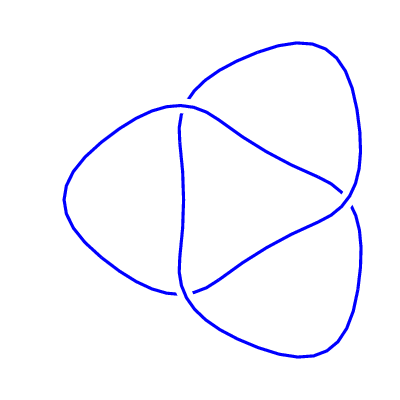
\includegraphics[width=\linewidth]{../data/3_1.png}
        \subcaption{$3_{1}$}
    \end{minipage}
    \begin{minipage}[b]{.18\linewidth}
        \centering
        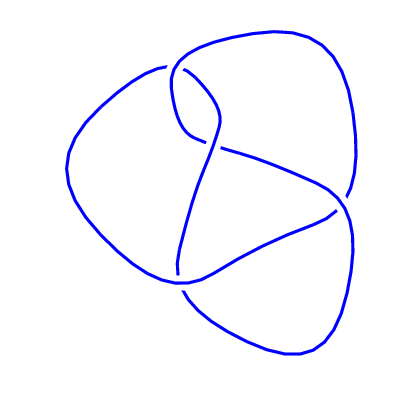
\includegraphics[width=\linewidth]{../data/4_1.png}
        \subcaption{$4_{1}$}
    \end{minipage}
    \begin{minipage}[b]{.18\linewidth}
        \centering
        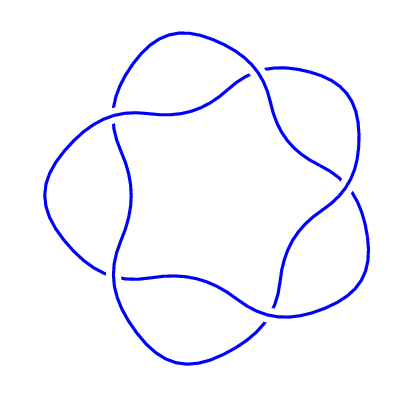
\includegraphics[width=\linewidth]{../data/5_1.png}
        \subcaption{$5_{1}$}
    \end{minipage}
    \begin{minipage}[b]{.18\linewidth}
        \centering
        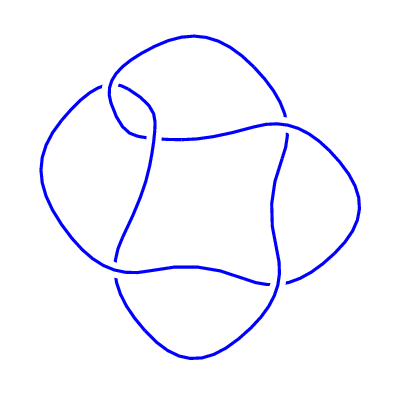
\includegraphics[width=\linewidth]{../data/5_2.png}
        \subcaption{$5_{2}$}
    \end{minipage}
    \begin{minipage}[b]{.18\linewidth}
        \centering
        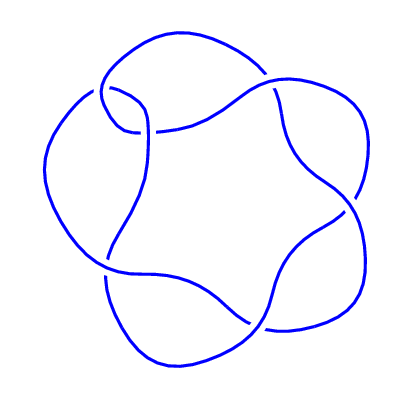
\includegraphics[width=\linewidth]{../data/6_1.png}
        \subcaption{$6_{1}$}
    \end{minipage}
\end{figure}
\begin{figure}[H]
    \begin{minipage}[b]{.18\linewidth}
        \centering
        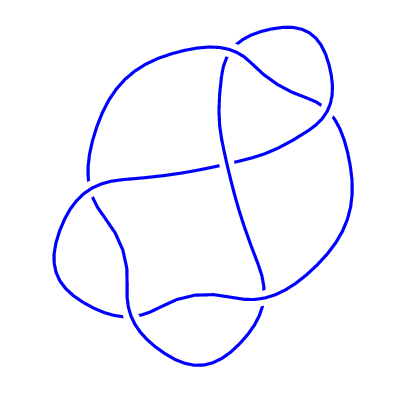
\includegraphics[width=\linewidth]{../data/6_2.png}
        \subcaption{$6_{2}$}
    \end{minipage}
    \begin{minipage}[b]{.18\linewidth}
        \centering
        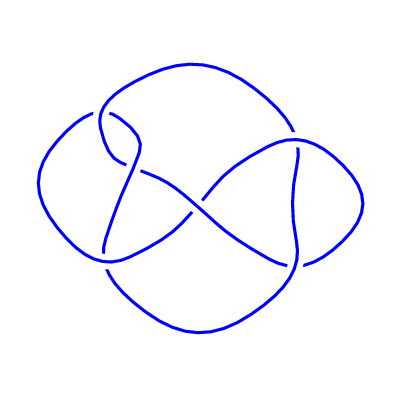
\includegraphics[width=\linewidth]{../data/6_3.png}
        \subcaption{$6_{3}$}
    \end{minipage}
    \begin{minipage}[b]{.18\linewidth}
        \centering
        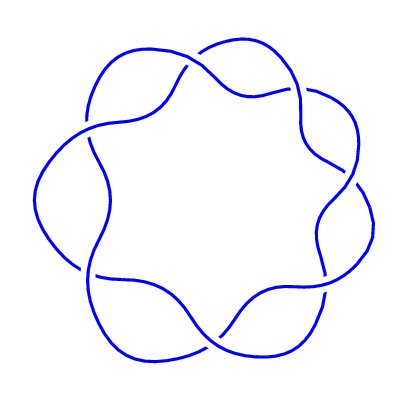
\includegraphics[width=\linewidth]{../data/7_1.png}
        \subcaption{$7_{1}$}
    \end{minipage}
    \begin{minipage}[b]{.18\linewidth}
        \centering
        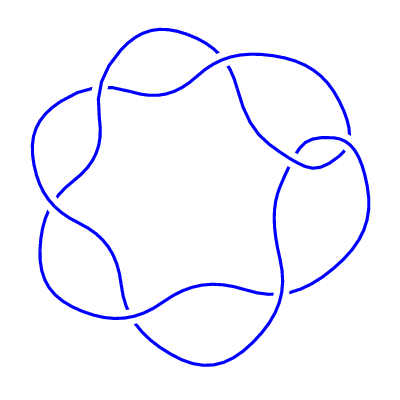
\includegraphics[width=\linewidth]{../data/7_2.png}
        \subcaption{$7_{2}$}
    \end{minipage}
    \begin{minipage}[b]{.18\linewidth}
        \centering
        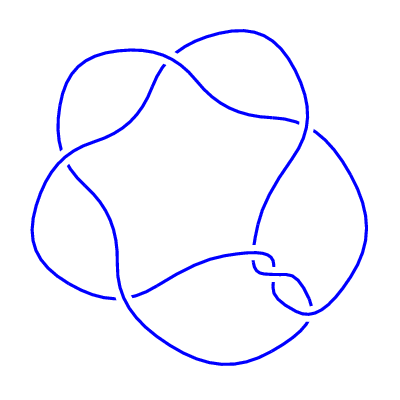
\includegraphics[width=\linewidth]{../data/7_3.png}
        \subcaption{$7_{3}$}
    \end{minipage}
\end{figure}
\begin{figure}[H]
    \begin{minipage}[b]{.18\linewidth}
        \centering
        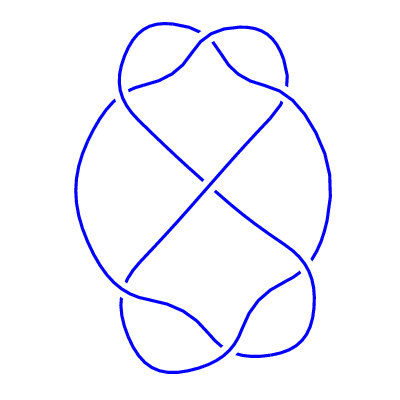
\includegraphics[width=\linewidth]{../data/7_4.png}
        \subcaption{$7_{4}$}
    \end{minipage}
    \begin{minipage}[b]{.18\linewidth}
        \centering
        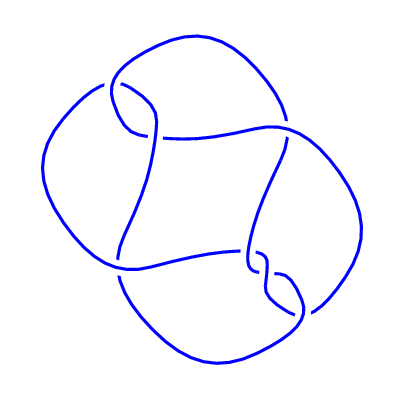
\includegraphics[width=\linewidth]{../data/7_5.png}
        \subcaption{$7_{5}$}
    \end{minipage}
    \begin{minipage}[b]{.18\linewidth}
        \centering
        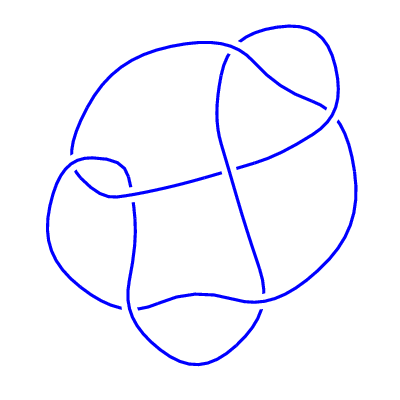
\includegraphics[width=\linewidth]{../data/7_6.png}
        \subcaption{$7_{6}$}
    \end{minipage}
    \begin{minipage}[b]{.18\linewidth}
        \centering
        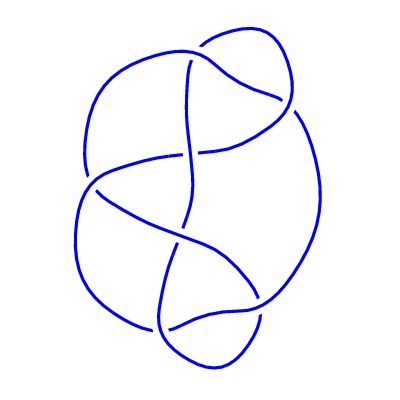
\includegraphics[width=\linewidth]{../data/7_7.png}
        \subcaption{$7_{7}$}
    \end{minipage}
    \begin{minipage}[b]{.18\linewidth}
        \centering
        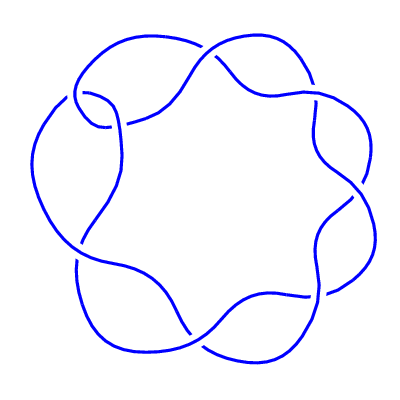
\includegraphics[width=\linewidth]{../data/8_1.png}
        \subcaption{$8_{1}$}
    \end{minipage}
\end{figure}
\begin{figure}[H]
    \begin{minipage}[b]{.18\linewidth}
        \centering
        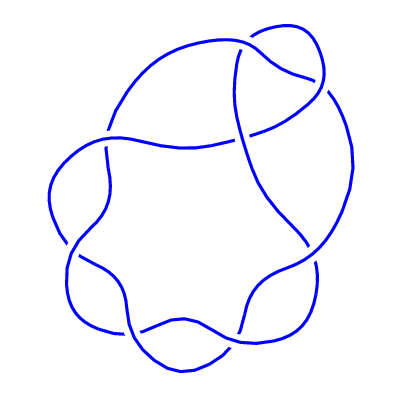
\includegraphics[width=\linewidth]{../data/8_2.png}
        \subcaption{$8_{2}$}
    \end{minipage}
    \begin{minipage}[b]{.18\linewidth}
        \centering
        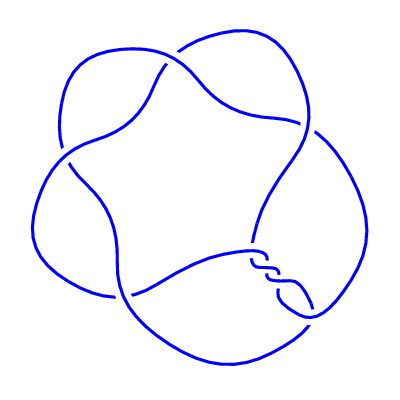
\includegraphics[width=\linewidth]{../data/8_3.png}
        \subcaption{$8_{3}$}
    \end{minipage}
    \begin{minipage}[b]{.18\linewidth}
        \centering
        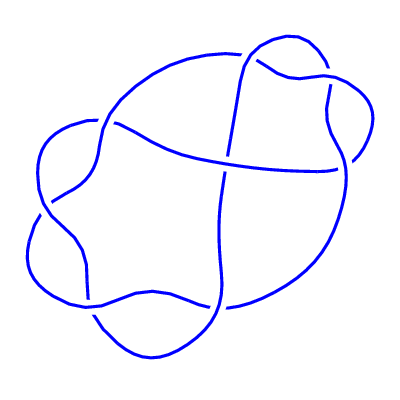
\includegraphics[width=\linewidth]{../data/8_4.png}
        \subcaption{$8_{4}$}
    \end{minipage}
    \begin{minipage}[b]{.18\linewidth}
        \centering
        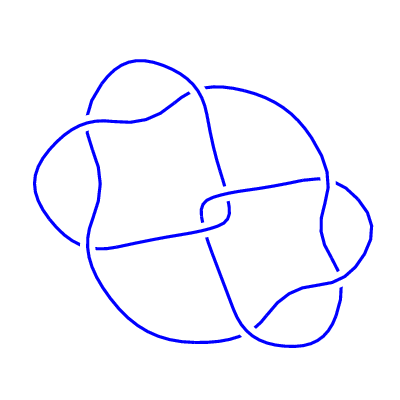
\includegraphics[width=\linewidth]{../data/8_5.png}
        \subcaption{$8_{5}$}
    \end{minipage}
    \begin{minipage}[b]{.18\linewidth}
        \centering
        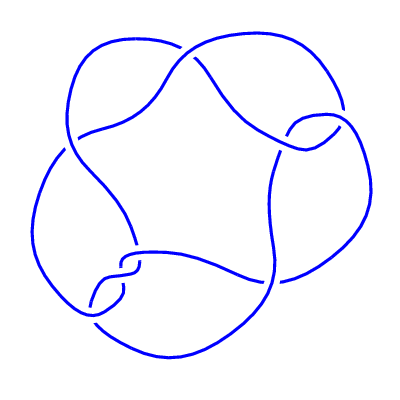
\includegraphics[width=\linewidth]{../data/8_6.png}
        \subcaption{$8_{6}$}
    \end{minipage}
\end{figure}
\begin{figure}[H]
    \begin{minipage}[b]{.18\linewidth}
        \centering
        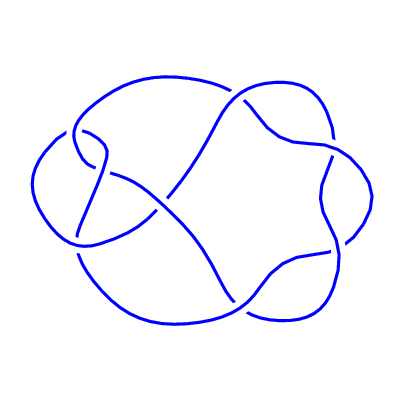
\includegraphics[width=\linewidth]{../data/8_7.png}
        \subcaption{$8_{7}$}
    \end{minipage}
    \begin{minipage}[b]{.18\linewidth}
        \centering
        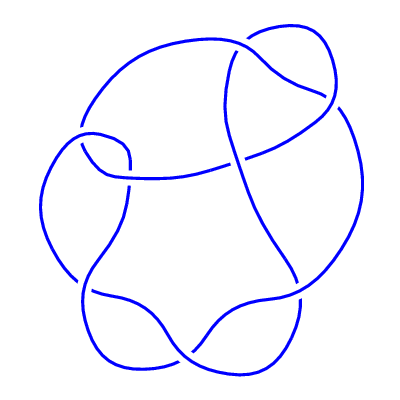
\includegraphics[width=\linewidth]{../data/8_8.png}
        \subcaption{$8_{8}$}
    \end{minipage}
    \begin{minipage}[b]{.18\linewidth}
        \centering
        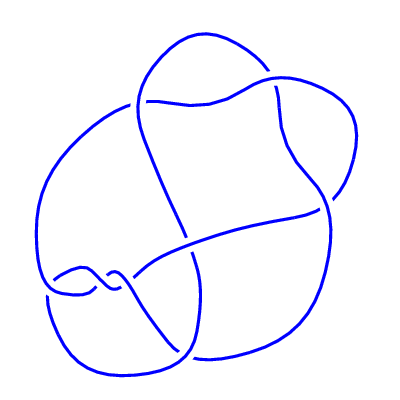
\includegraphics[width=\linewidth]{../data/8_9.png}
        \subcaption{$8_{9}$}
    \end{minipage}
    \begin{minipage}[b]{.18\linewidth}
        \centering
        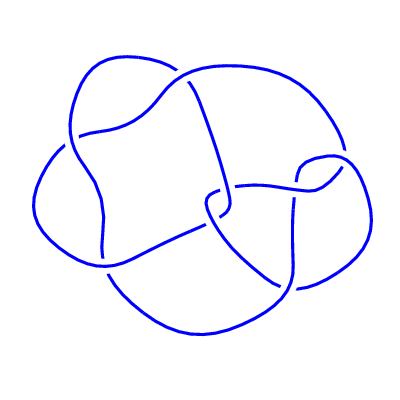
\includegraphics[width=\linewidth]{../data/8_10.png}
        \subcaption{$8_{10}$}
    \end{minipage}
    \begin{minipage}[b]{.18\linewidth}
        \centering
        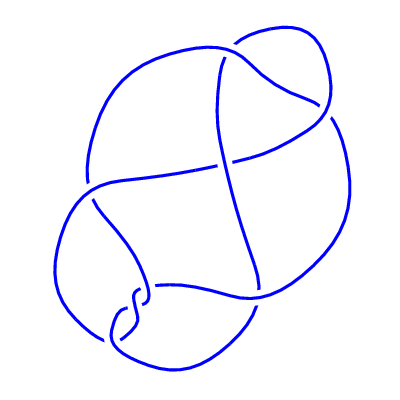
\includegraphics[width=\linewidth]{../data/8_11.png}
        \subcaption{$8_{11}$}
    \end{minipage}
\end{figure}
\begin{figure}[H]
    \begin{minipage}[b]{.18\linewidth}
        \centering
        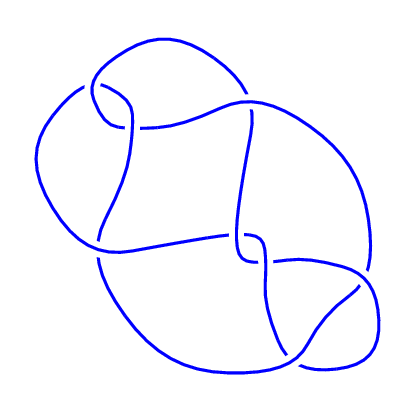
\includegraphics[width=\linewidth]{../data/8_12.png}
        \subcaption{$8_{12}$}
    \end{minipage}
    \begin{minipage}[b]{.18\linewidth}
        \centering
        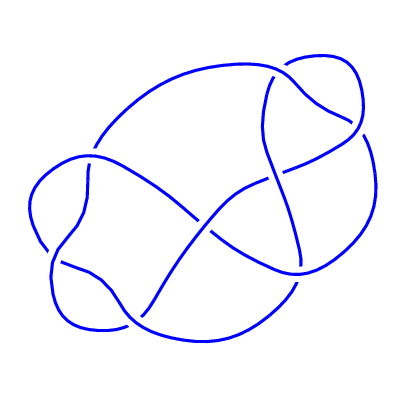
\includegraphics[width=\linewidth]{../data/8_13.png}
        \subcaption{$8_{13}$}
    \end{minipage}
    \begin{minipage}[b]{.18\linewidth}
        \centering
        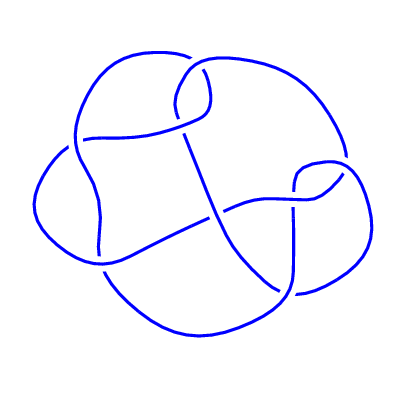
\includegraphics[width=\linewidth]{../data/8_14.png}
        \subcaption{$8_{14}$}
    \end{minipage}
    \begin{minipage}[b]{.18\linewidth}
        \centering
        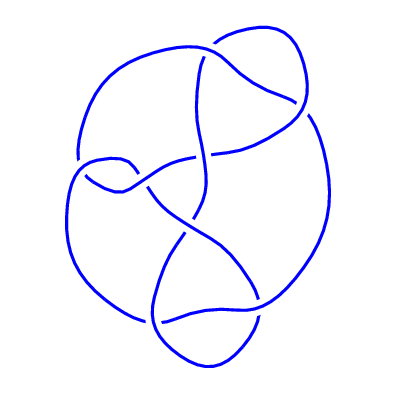
\includegraphics[width=\linewidth]{../data/8_15.png}
        \subcaption{$8_{15}$}
    \end{minipage}
    \begin{minipage}[b]{.18\linewidth}
        \centering
        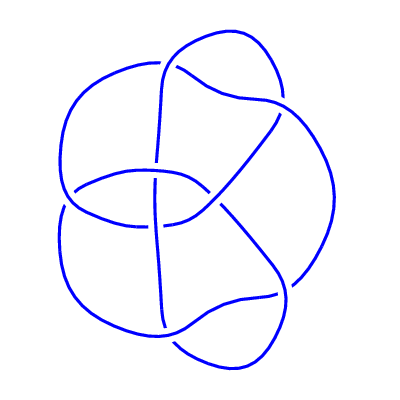
\includegraphics[width=\linewidth]{../data/8_16.png}
        \subcaption{$8_{16}$}
    \end{minipage}
\end{figure}
\begin{figure}[H]
    \begin{minipage}[b]{.18\linewidth}
        \centering
        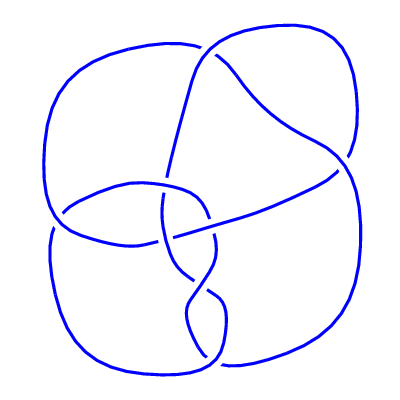
\includegraphics[width=\linewidth]{../data/8_17.png}
        \subcaption{$8_{17}$}
    \end{minipage}
    \begin{minipage}[b]{.18\linewidth}
        \centering
        \includegraphics[width=\linewidth]{../data/8_18.png}
        \subcaption{$8_{18}$}
    \end{minipage}
    \begin{minipage}[b]{.18\linewidth}
        \centering
        \includegraphics[width=\linewidth]{../data/8_19.png}
        \subcaption{$8_{19}$}
    \end{minipage}
    \begin{minipage}[b]{.18\linewidth}
        \centering
        \includegraphics[width=\linewidth]{../data/8_20.png}
        \subcaption{$8_{20}$}
    \end{minipage}
    \begin{minipage}[b]{.18\linewidth}
        \centering
        \includegraphics[width=\linewidth]{../data/8_21.png}
        \subcaption{$8_{21}$}
    \end{minipage}
\end{figure}
\begin{figure}[H]
    \begin{minipage}[b]{.18\linewidth}
        \centering
        \includegraphics[width=\linewidth]{../data/9_1.png}
        \subcaption{$9_{1}$}
    \end{minipage}
    \begin{minipage}[b]{.18\linewidth}
        \centering
        \includegraphics[width=\linewidth]{../data/9_2.png}
        \subcaption{$9_{2}$}
    \end{minipage}
    \begin{minipage}[b]{.18\linewidth}
        \centering
        \includegraphics[width=\linewidth]{../data/9_3.png}
        \subcaption{$9_{3}$}
    \end{minipage}
    \begin{minipage}[b]{.18\linewidth}
        \centering
        \includegraphics[width=\linewidth]{../data/9_4.png}
        \subcaption{$9_{4}$}
    \end{minipage}
    \begin{minipage}[b]{.18\linewidth}
        \centering
        \includegraphics[width=\linewidth]{../data/9_5.png}
        \subcaption{$9_{5}$}
    \end{minipage}
\end{figure}
\begin{figure}[H]
    \begin{minipage}[b]{.18\linewidth}
        \centering
        \includegraphics[width=\linewidth]{../data/9_6.png}
        \subcaption{$9_{6}$}
    \end{minipage}
    \begin{minipage}[b]{.18\linewidth}
        \centering
        \includegraphics[width=\linewidth]{../data/9_7.png}
        \subcaption{$9_{7}$}
    \end{minipage}
    \begin{minipage}[b]{.18\linewidth}
        \centering
        \includegraphics[width=\linewidth]{../data/9_8.png}
        \subcaption{$9_{8}$}
    \end{minipage}
    \begin{minipage}[b]{.18\linewidth}
        \centering
        \includegraphics[width=\linewidth]{../data/9_9.png}
        \subcaption{$9_{9}$}
    \end{minipage}
    \begin{minipage}[b]{.18\linewidth}
        \centering
        \includegraphics[width=\linewidth]{../data/9_10.png}
        \subcaption{$9_{10}$}
    \end{minipage}
\end{figure}
\begin{figure}[H]
    \begin{minipage}[b]{.18\linewidth}
        \centering
        \includegraphics[width=\linewidth]{../data/9_11.png}
        \subcaption{$9_{11}$}
    \end{minipage}
    \begin{minipage}[b]{.18\linewidth}
        \centering
        \includegraphics[width=\linewidth]{../data/9_12.png}
        \subcaption{$9_{12}$}
    \end{minipage}
    \begin{minipage}[b]{.18\linewidth}
        \centering
        \includegraphics[width=\linewidth]{../data/9_13.png}
        \subcaption{$9_{13}$}
    \end{minipage}
    \begin{minipage}[b]{.18\linewidth}
        \centering
        \includegraphics[width=\linewidth]{../data/9_14.png}
        \subcaption{$9_{14}$}
    \end{minipage}
    \begin{minipage}[b]{.18\linewidth}
        \centering
        \includegraphics[width=\linewidth]{../data/9_15.png}
        \subcaption{$9_{15}$}
    \end{minipage}
\end{figure}
\begin{figure}[H]
    \begin{minipage}[b]{.18\linewidth}
        \centering
        \includegraphics[width=\linewidth]{../data/9_16.png}
        \subcaption{$9_{16}$}
    \end{minipage}
    \begin{minipage}[b]{.18\linewidth}
        \centering
        \includegraphics[width=\linewidth]{../data/9_17.png}
        \subcaption{$9_{17}$}
    \end{minipage}
    \begin{minipage}[b]{.18\linewidth}
        \centering
        \includegraphics[width=\linewidth]{../data/9_18.png}
        \subcaption{$9_{18}$}
    \end{minipage}
    \begin{minipage}[b]{.18\linewidth}
        \centering
        \includegraphics[width=\linewidth]{../data/9_19.png}
        \subcaption{$9_{19}$}
    \end{minipage}
    \begin{minipage}[b]{.18\linewidth}
        \centering
        \includegraphics[width=\linewidth]{../data/9_20.png}
        \subcaption{$9_{20}$}
    \end{minipage}
\end{figure}
\begin{figure}[H]
    \begin{minipage}[b]{.18\linewidth}
        \centering
        \includegraphics[width=\linewidth]{../data/9_21.png}
        \subcaption{$9_{21}$}
    \end{minipage}
    \begin{minipage}[b]{.18\linewidth}
        \centering
        \includegraphics[width=\linewidth]{../data/9_22.png}
        \subcaption{$9_{22}$}
    \end{minipage}
    \begin{minipage}[b]{.18\linewidth}
        \centering
        \includegraphics[width=\linewidth]{../data/9_23.png}
        \subcaption{$9_{23}$}
    \end{minipage}
    \begin{minipage}[b]{.18\linewidth}
        \centering
        \includegraphics[width=\linewidth]{../data/9_24.png}
        \subcaption{$9_{24}$}
    \end{minipage}
    \begin{minipage}[b]{.18\linewidth}
        \centering
        \includegraphics[width=\linewidth]{../data/9_25.png}
        \subcaption{$9_{25}$}
    \end{minipage}
\end{figure}
\begin{figure}[H]
    \begin{minipage}[b]{.18\linewidth}
        \centering
        \includegraphics[width=\linewidth]{../data/9_26.png}
        \subcaption{$9_{26}$}
    \end{minipage}
    \begin{minipage}[b]{.18\linewidth}
        \centering
        \includegraphics[width=\linewidth]{../data/9_27.png}
        \subcaption{$9_{27}$}
    \end{minipage}
    \begin{minipage}[b]{.18\linewidth}
        \centering
        \includegraphics[width=\linewidth]{../data/9_28.png}
        \subcaption{$9_{28}$}
    \end{minipage}
    \begin{minipage}[b]{.18\linewidth}
        \centering
        \includegraphics[width=\linewidth]{../data/9_29.png}
        \subcaption{$9_{29}$}
    \end{minipage}
    \begin{minipage}[b]{.18\linewidth}
        \centering
        \includegraphics[width=\linewidth]{../data/9_30.png}
        \subcaption{$9_{30}$}
    \end{minipage}
\end{figure}
\begin{figure}[H]
    \begin{minipage}[b]{.18\linewidth}
        \centering
        \includegraphics[width=\linewidth]{../data/9_31.png}
        \subcaption{$9_{31}$}
    \end{minipage}
    \begin{minipage}[b]{.18\linewidth}
        \centering
        \includegraphics[width=\linewidth]{../data/9_32.png}
        \subcaption{$9_{32}$}
    \end{minipage}
    \begin{minipage}[b]{.18\linewidth}
        \centering
        \includegraphics[width=\linewidth]{../data/9_33.png}
        \subcaption{$9_{33}$}
    \end{minipage}
    \begin{minipage}[b]{.18\linewidth}
        \centering
        \includegraphics[width=\linewidth]{../data/9_34.png}
        \subcaption{$9_{34}$}
    \end{minipage}
    \begin{minipage}[b]{.18\linewidth}
        \centering
        \includegraphics[width=\linewidth]{../data/9_35.png}
        \subcaption{$9_{35}$}
    \end{minipage}
\end{figure}
\begin{figure}[H]
    \begin{minipage}[b]{.18\linewidth}
        \centering
        \includegraphics[width=\linewidth]{../data/9_36.png}
        \subcaption{$9_{36}$}
    \end{minipage}
    \begin{minipage}[b]{.18\linewidth}
        \centering
        \includegraphics[width=\linewidth]{../data/9_37.png}
        \subcaption{$9_{37}$}
    \end{minipage}
    \begin{minipage}[b]{.18\linewidth}
        \centering
        \includegraphics[width=\linewidth]{../data/9_38.png}
        \subcaption{$9_{38}$}
    \end{minipage}
    \begin{minipage}[b]{.18\linewidth}
        \centering
        \includegraphics[width=\linewidth]{../data/9_39.png}
        \subcaption{$9_{39}$}
    \end{minipage}
    \begin{minipage}[b]{.18\linewidth}
        \centering
        \includegraphics[width=\linewidth]{../data/9_40.png}
        \subcaption{$9_{40}$}
    \end{minipage}
\end{figure}
\begin{figure}[H]
    \begin{minipage}[b]{.18\linewidth}
        \centering
        \includegraphics[width=\linewidth]{../data/9_41.png}
        \subcaption{$9_{41}$}
    \end{minipage}
    \begin{minipage}[b]{.18\linewidth}
        \centering
        \includegraphics[width=\linewidth]{../data/9_42.png}
        \subcaption{$9_{42}$}
    \end{minipage}
    \begin{minipage}[b]{.18\linewidth}
        \centering
        \includegraphics[width=\linewidth]{../data/9_43.png}
        \subcaption{$9_{43}$}
    \end{minipage}
    \begin{minipage}[b]{.18\linewidth}
        \centering
        \includegraphics[width=\linewidth]{../data/9_44.png}
        \subcaption{$9_{44}$}
    \end{minipage}
    \begin{minipage}[b]{.18\linewidth}
        \centering
        \includegraphics[width=\linewidth]{../data/9_45.png}
        \subcaption{$9_{45}$}
    \end{minipage}
\end{figure}
\begin{figure}[H]
    \begin{minipage}[b]{.18\linewidth}
        \centering
        \includegraphics[width=\linewidth]{../data/9_46.png}
        \subcaption{$9_{46}$}
    \end{minipage}
    \begin{minipage}[b]{.18\linewidth}
        \centering
        \includegraphics[width=\linewidth]{../data/9_47.png}
        \subcaption{$9_{47}$}
    \end{minipage}
    \begin{minipage}[b]{.18\linewidth}
        \centering
        \includegraphics[width=\linewidth]{../data/9_48.png}
        \subcaption{$9_{48}$}
    \end{minipage}
    \begin{minipage}[b]{.18\linewidth}
        \centering
        \includegraphics[width=\linewidth]{../data/9_49.png}
        \subcaption{$9_{49}$}
    \end{minipage}
    \begin{minipage}[b]{.18\linewidth}
        \centering
        \includegraphics[width=\linewidth]{../data/10_1.png}
        \subcaption{$10_{1}$}
    \end{minipage}
\end{figure}
\begin{figure}[H]
    \begin{minipage}[b]{.18\linewidth}
        \centering
        \includegraphics[width=\linewidth]{../data/10_2.png}
        \subcaption{$10_{2}$}
    \end{minipage}
    \begin{minipage}[b]{.18\linewidth}
        \centering
        \includegraphics[width=\linewidth]{../data/10_3.png}
        \subcaption{$10_{3}$}
    \end{minipage}
    \begin{minipage}[b]{.18\linewidth}
        \centering
        \includegraphics[width=\linewidth]{../data/10_4.png}
        \subcaption{$10_{4}$}
    \end{minipage}
    \begin{minipage}[b]{.18\linewidth}
        \centering
        \includegraphics[width=\linewidth]{../data/10_5.png}
        \subcaption{$10_{5}$}
    \end{minipage}
    \begin{minipage}[b]{.18\linewidth}
        \centering
        \includegraphics[width=\linewidth]{../data/10_6.png}
        \subcaption{$10_{6}$}
    \end{minipage}
\end{figure}
\begin{figure}[H]
    \begin{minipage}[b]{.18\linewidth}
        \centering
        \includegraphics[width=\linewidth]{../data/10_7.png}
        \subcaption{$10_{7}$}
    \end{minipage}
    \begin{minipage}[b]{.18\linewidth}
        \centering
        \includegraphics[width=\linewidth]{../data/10_8.png}
        \subcaption{$10_{8}$}
    \end{minipage}
    \begin{minipage}[b]{.18\linewidth}
        \centering
        \includegraphics[width=\linewidth]{../data/10_9.png}
        \subcaption{$10_{9}$}
    \end{minipage}
    \begin{minipage}[b]{.18\linewidth}
        \centering
        \includegraphics[width=\linewidth]{../data/10_10.png}
        \subcaption{$10_{10}$}
    \end{minipage}
    \begin{minipage}[b]{.18\linewidth}
        \centering
        \includegraphics[width=\linewidth]{../data/10_11.png}
        \subcaption{$10_{11}$}
    \end{minipage}
\end{figure}
\begin{figure}[H]
    \begin{minipage}[b]{.18\linewidth}
        \centering
        \includegraphics[width=\linewidth]{../data/10_12.png}
        \subcaption{$10_{12}$}
    \end{minipage}
    \begin{minipage}[b]{.18\linewidth}
        \centering
        \includegraphics[width=\linewidth]{../data/10_13.png}
        \subcaption{$10_{13}$}
    \end{minipage}
    \begin{minipage}[b]{.18\linewidth}
        \centering
        \includegraphics[width=\linewidth]{../data/10_14.png}
        \subcaption{$10_{14}$}
    \end{minipage}
    \begin{minipage}[b]{.18\linewidth}
        \centering
        \includegraphics[width=\linewidth]{../data/10_15.png}
        \subcaption{$10_{15}$}
    \end{minipage}
    \begin{minipage}[b]{.18\linewidth}
        \centering
        \includegraphics[width=\linewidth]{../data/10_16.png}
        \subcaption{$10_{16}$}
    \end{minipage}
\end{figure}
\begin{figure}[H]
    \begin{minipage}[b]{.18\linewidth}
        \centering
        \includegraphics[width=\linewidth]{../data/10_17.png}
        \subcaption{$10_{17}$}
    \end{minipage}
    \begin{minipage}[b]{.18\linewidth}
        \centering
        \includegraphics[width=\linewidth]{../data/10_18.png}
        \subcaption{$10_{18}$}
    \end{minipage}
    \begin{minipage}[b]{.18\linewidth}
        \centering
        \includegraphics[width=\linewidth]{../data/10_19.png}
        \subcaption{$10_{19}$}
    \end{minipage}
    \begin{minipage}[b]{.18\linewidth}
        \centering
        \includegraphics[width=\linewidth]{../data/10_20.png}
        \subcaption{$10_{20}$}
    \end{minipage}
    \begin{minipage}[b]{.18\linewidth}
        \centering
        \includegraphics[width=\linewidth]{../data/10_21.png}
        \subcaption{$10_{21}$}
    \end{minipage}
\end{figure}
\begin{figure}[H]
    \begin{minipage}[b]{.18\linewidth}
        \centering
        \includegraphics[width=\linewidth]{../data/10_22.png}
        \subcaption{$10_{22}$}
    \end{minipage}
    \begin{minipage}[b]{.18\linewidth}
        \centering
        \includegraphics[width=\linewidth]{../data/10_23.png}
        \subcaption{$10_{23}$}
    \end{minipage}
    \begin{minipage}[b]{.18\linewidth}
        \centering
        \includegraphics[width=\linewidth]{../data/10_24.png}
        \subcaption{$10_{24}$}
    \end{minipage}
    \begin{minipage}[b]{.18\linewidth}
        \centering
        \includegraphics[width=\linewidth]{../data/10_25.png}
        \subcaption{$10_{25}$}
    \end{minipage}
    \begin{minipage}[b]{.18\linewidth}
        \centering
        \includegraphics[width=\linewidth]{../data/10_26.png}
        \subcaption{$10_{26}$}
    \end{minipage}
\end{figure}
\begin{figure}[H]
    \begin{minipage}[b]{.18\linewidth}
        \centering
        \includegraphics[width=\linewidth]{../data/10_27.png}
        \subcaption{$10_{27}$}
    \end{minipage}
    \begin{minipage}[b]{.18\linewidth}
        \centering
        \includegraphics[width=\linewidth]{../data/10_28.png}
        \subcaption{$10_{28}$}
    \end{minipage}
    \begin{minipage}[b]{.18\linewidth}
        \centering
        \includegraphics[width=\linewidth]{../data/10_29.png}
        \subcaption{$10_{29}$}
    \end{minipage}
    \begin{minipage}[b]{.18\linewidth}
        \centering
        \includegraphics[width=\linewidth]{../data/10_30.png}
        \subcaption{$10_{30}$}
    \end{minipage}
    \begin{minipage}[b]{.18\linewidth}
        \centering
        \includegraphics[width=\linewidth]{../data/10_31.png}
        \subcaption{$10_{31}$}
    \end{minipage}
\end{figure}
\begin{figure}[H]
    \begin{minipage}[b]{.18\linewidth}
        \centering
        \includegraphics[width=\linewidth]{../data/10_32.png}
        \subcaption{$10_{32}$}
    \end{minipage}
    \begin{minipage}[b]{.18\linewidth}
        \centering
        \includegraphics[width=\linewidth]{../data/10_33.png}
        \subcaption{$10_{33}$}
    \end{minipage}
    \begin{minipage}[b]{.18\linewidth}
        \centering
        \includegraphics[width=\linewidth]{../data/10_34.png}
        \subcaption{$10_{34}$}
    \end{minipage}
    \begin{minipage}[b]{.18\linewidth}
        \centering
        \includegraphics[width=\linewidth]{../data/10_35.png}
        \subcaption{$10_{35}$}
    \end{minipage}
    \begin{minipage}[b]{.18\linewidth}
        \centering
        \includegraphics[width=\linewidth]{../data/10_36.png}
        \subcaption{$10_{36}$}
    \end{minipage}
\end{figure}
\begin{figure}[H]
    \begin{minipage}[b]{.18\linewidth}
        \centering
        \includegraphics[width=\linewidth]{../data/10_37.png}
        \subcaption{$10_{37}$}
    \end{minipage}
    \begin{minipage}[b]{.18\linewidth}
        \centering
        \includegraphics[width=\linewidth]{../data/10_38.png}
        \subcaption{$10_{38}$}
    \end{minipage}
    \begin{minipage}[b]{.18\linewidth}
        \centering
        \includegraphics[width=\linewidth]{../data/10_39.png}
        \subcaption{$10_{39}$}
    \end{minipage}
    \begin{minipage}[b]{.18\linewidth}
        \centering
        \includegraphics[width=\linewidth]{../data/10_40.png}
        \subcaption{$10_{40}$}
    \end{minipage}
    \begin{minipage}[b]{.18\linewidth}
        \centering
        \includegraphics[width=\linewidth]{../data/10_41.png}
        \subcaption{$10_{41}$}
    \end{minipage}
\end{figure}
\begin{figure}[H]
    \begin{minipage}[b]{.18\linewidth}
        \centering
        \includegraphics[width=\linewidth]{../data/10_42.png}
        \subcaption{$10_{42}$}
    \end{minipage}
    \begin{minipage}[b]{.18\linewidth}
        \centering
        \includegraphics[width=\linewidth]{../data/10_43.png}
        \subcaption{$10_{43}$}
    \end{minipage}
    \begin{minipage}[b]{.18\linewidth}
        \centering
        \includegraphics[width=\linewidth]{../data/10_44.png}
        \subcaption{$10_{44}$}
    \end{minipage}
    \begin{minipage}[b]{.18\linewidth}
        \centering
        \includegraphics[width=\linewidth]{../data/10_45.png}
        \subcaption{$10_{45}$}
    \end{minipage}
    \begin{minipage}[b]{.18\linewidth}
        \centering
        \includegraphics[width=\linewidth]{../data/10_46.png}
        \subcaption{$10_{46}$}
    \end{minipage}
\end{figure}
\begin{figure}[H]
    \begin{minipage}[b]{.18\linewidth}
        \centering
        \includegraphics[width=\linewidth]{../data/10_47.png}
        \subcaption{$10_{47}$}
    \end{minipage}
    \begin{minipage}[b]{.18\linewidth}
        \centering
        \includegraphics[width=\linewidth]{../data/10_48.png}
        \subcaption{$10_{48}$}
    \end{minipage}
    \begin{minipage}[b]{.18\linewidth}
        \centering
        \includegraphics[width=\linewidth]{../data/10_49.png}
        \subcaption{$10_{49}$}
    \end{minipage}
    \begin{minipage}[b]{.18\linewidth}
        \centering
        \includegraphics[width=\linewidth]{../data/10_50.png}
        \subcaption{$10_{50}$}
    \end{minipage}
    \begin{minipage}[b]{.18\linewidth}
        \centering
        \includegraphics[width=\linewidth]{../data/10_51.png}
        \subcaption{$10_{51}$}
    \end{minipage}
\end{figure}
\begin{figure}[H]
    \begin{minipage}[b]{.18\linewidth}
        \centering
        \includegraphics[width=\linewidth]{../data/10_52.png}
        \subcaption{$10_{52}$}
    \end{minipage}
    \begin{minipage}[b]{.18\linewidth}
        \centering
        \includegraphics[width=\linewidth]{../data/10_53.png}
        \subcaption{$10_{53}$}
    \end{minipage}
    \begin{minipage}[b]{.18\linewidth}
        \centering
        \includegraphics[width=\linewidth]{../data/10_54.png}
        \subcaption{$10_{54}$}
    \end{minipage}
    \begin{minipage}[b]{.18\linewidth}
        \centering
        \includegraphics[width=\linewidth]{../data/10_55.png}
        \subcaption{$10_{55}$}
    \end{minipage}
    \begin{minipage}[b]{.18\linewidth}
        \centering
        \includegraphics[width=\linewidth]{../data/10_56.png}
        \subcaption{$10_{56}$}
    \end{minipage}
\end{figure}
\begin{figure}[H]
    \begin{minipage}[b]{.18\linewidth}
        \centering
        \includegraphics[width=\linewidth]{../data/10_57.png}
        \subcaption{$10_{57}$}
    \end{minipage}
    \begin{minipage}[b]{.18\linewidth}
        \centering
        \includegraphics[width=\linewidth]{../data/10_58.png}
        \subcaption{$10_{58}$}
    \end{minipage}
    \begin{minipage}[b]{.18\linewidth}
        \centering
        \includegraphics[width=\linewidth]{../data/10_59.png}
        \subcaption{$10_{59}$}
    \end{minipage}
    \begin{minipage}[b]{.18\linewidth}
        \centering
        \includegraphics[width=\linewidth]{../data/10_60.png}
        \subcaption{$10_{60}$}
    \end{minipage}
    \begin{minipage}[b]{.18\linewidth}
        \centering
        \includegraphics[width=\linewidth]{../data/10_61.png}
        \subcaption{$10_{61}$}
    \end{minipage}
\end{figure}
\begin{figure}[H]
    \begin{minipage}[b]{.18\linewidth}
        \centering
        \includegraphics[width=\linewidth]{../data/10_62.png}
        \subcaption{$10_{62}$}
    \end{minipage}
    \begin{minipage}[b]{.18\linewidth}
        \centering
        \includegraphics[width=\linewidth]{../data/10_63.png}
        \subcaption{$10_{63}$}
    \end{minipage}
    \begin{minipage}[b]{.18\linewidth}
        \centering
        \includegraphics[width=\linewidth]{../data/10_64.png}
        \subcaption{$10_{64}$}
    \end{minipage}
    \begin{minipage}[b]{.18\linewidth}
        \centering
        \includegraphics[width=\linewidth]{../data/10_65.png}
        \subcaption{$10_{65}$}
    \end{minipage}
    \begin{minipage}[b]{.18\linewidth}
        \centering
        \includegraphics[width=\linewidth]{../data/10_66.png}
        \subcaption{$10_{66}$}
    \end{minipage}
\end{figure}
\begin{figure}[H]
    \begin{minipage}[b]{.18\linewidth}
        \centering
        \includegraphics[width=\linewidth]{../data/10_67.png}
        \subcaption{$10_{67}$}
    \end{minipage}
    \begin{minipage}[b]{.18\linewidth}
        \centering
        \includegraphics[width=\linewidth]{../data/10_68.png}
        \subcaption{$10_{68}$}
    \end{minipage}
    \begin{minipage}[b]{.18\linewidth}
        \centering
        \includegraphics[width=\linewidth]{../data/10_69.png}
        \subcaption{$10_{69}$}
    \end{minipage}
    \begin{minipage}[b]{.18\linewidth}
        \centering
        \includegraphics[width=\linewidth]{../data/10_70.png}
        \subcaption{$10_{70}$}
    \end{minipage}
    \begin{minipage}[b]{.18\linewidth}
        \centering
        \includegraphics[width=\linewidth]{../data/10_71.png}
        \subcaption{$10_{71}$}
    \end{minipage}
\end{figure}
\begin{figure}[H]
    \begin{minipage}[b]{.18\linewidth}
        \centering
        \includegraphics[width=\linewidth]{../data/10_72.png}
        \subcaption{$10_{72}$}
    \end{minipage}
    \begin{minipage}[b]{.18\linewidth}
        \centering
        \includegraphics[width=\linewidth]{../data/10_73.png}
        \subcaption{$10_{73}$}
    \end{minipage}
    \begin{minipage}[b]{.18\linewidth}
        \centering
        \includegraphics[width=\linewidth]{../data/10_74.png}
        \subcaption{$10_{74}$}
    \end{minipage}
    \begin{minipage}[b]{.18\linewidth}
        \centering
        \includegraphics[width=\linewidth]{../data/10_75.png}
        \subcaption{$10_{75}$}
    \end{minipage}
    \begin{minipage}[b]{.18\linewidth}
        \centering
        \includegraphics[width=\linewidth]{../data/10_76.png}
        \subcaption{$10_{76}$}
    \end{minipage}
\end{figure}
\begin{figure}[H]
    \begin{minipage}[b]{.18\linewidth}
        \centering
        \includegraphics[width=\linewidth]{../data/10_77.png}
        \subcaption{$10_{77}$}
    \end{minipage}
    \begin{minipage}[b]{.18\linewidth}
        \centering
        \includegraphics[width=\linewidth]{../data/10_78.png}
        \subcaption{$10_{78}$}
    \end{minipage}
    \begin{minipage}[b]{.18\linewidth}
        \centering
        \includegraphics[width=\linewidth]{../data/10_79.png}
        \subcaption{$10_{79}$}
    \end{minipage}
    \begin{minipage}[b]{.18\linewidth}
        \centering
        \includegraphics[width=\linewidth]{../data/10_80.png}
        \subcaption{$10_{80}$}
    \end{minipage}
    \begin{minipage}[b]{.18\linewidth}
        \centering
        \includegraphics[width=\linewidth]{../data/10_81.png}
        \subcaption{$10_{81}$}
    \end{minipage}
\end{figure}
\begin{figure}[H]
    \begin{minipage}[b]{.18\linewidth}
        \centering
        \includegraphics[width=\linewidth]{../data/10_82.png}
        \subcaption{$10_{82}$}
    \end{minipage}
    \begin{minipage}[b]{.18\linewidth}
        \centering
        \includegraphics[width=\linewidth]{../data/10_83.png}
        \subcaption{$10_{83}$}
    \end{minipage}
    \begin{minipage}[b]{.18\linewidth}
        \centering
        \includegraphics[width=\linewidth]{../data/10_84.png}
        \subcaption{$10_{84}$}
    \end{minipage}
    \begin{minipage}[b]{.18\linewidth}
        \centering
        \includegraphics[width=\linewidth]{../data/10_85.png}
        \subcaption{$10_{85}$}
    \end{minipage}
    \begin{minipage}[b]{.18\linewidth}
        \centering
        \includegraphics[width=\linewidth]{../data/10_86.png}
        \subcaption{$10_{86}$}
    \end{minipage}
\end{figure}
\begin{figure}[H]
    \begin{minipage}[b]{.18\linewidth}
        \centering
        \includegraphics[width=\linewidth]{../data/10_87.png}
        \subcaption{$10_{87}$}
    \end{minipage}
    \begin{minipage}[b]{.18\linewidth}
        \centering
        \includegraphics[width=\linewidth]{../data/10_88.png}
        \subcaption{$10_{88}$}
    \end{minipage}
    \begin{minipage}[b]{.18\linewidth}
        \centering
        \includegraphics[width=\linewidth]{../data/10_89.png}
        \subcaption{$10_{89}$}
    \end{minipage}
    \begin{minipage}[b]{.18\linewidth}
        \centering
        \includegraphics[width=\linewidth]{../data/10_90.png}
        \subcaption{$10_{90}$}
    \end{minipage}
    \begin{minipage}[b]{.18\linewidth}
        \centering
        \includegraphics[width=\linewidth]{../data/10_91.png}
        \subcaption{$10_{91}$}
    \end{minipage}
\end{figure}
\begin{figure}[H]
    \begin{minipage}[b]{.18\linewidth}
        \centering
        \includegraphics[width=\linewidth]{../data/10_92.png}
        \subcaption{$10_{92}$}
    \end{minipage}
    \begin{minipage}[b]{.18\linewidth}
        \centering
        \includegraphics[width=\linewidth]{../data/10_93.png}
        \subcaption{$10_{93}$}
    \end{minipage}
    \begin{minipage}[b]{.18\linewidth}
        \centering
        \includegraphics[width=\linewidth]{../data/10_94.png}
        \subcaption{$10_{94}$}
    \end{minipage}
    \begin{minipage}[b]{.18\linewidth}
        \centering
        \includegraphics[width=\linewidth]{../data/10_95.png}
        \subcaption{$10_{95}$}
    \end{minipage}
    \begin{minipage}[b]{.18\linewidth}
        \centering
        \includegraphics[width=\linewidth]{../data/10_96.png}
        \subcaption{$10_{96}$}
    \end{minipage}
\end{figure}
\begin{figure}[H]
    \begin{minipage}[b]{.18\linewidth}
        \centering
        \includegraphics[width=\linewidth]{../data/10_97.png}
        \subcaption{$10_{97}$}
    \end{minipage}
    \begin{minipage}[b]{.18\linewidth}
        \centering
        \includegraphics[width=\linewidth]{../data/10_98.png}
        \subcaption{$10_{98}$}
    \end{minipage}
    \begin{minipage}[b]{.18\linewidth}
        \centering
        \includegraphics[width=\linewidth]{../data/10_99.png}
        \subcaption{$10_{99}$}
    \end{minipage}
    \begin{minipage}[b]{.18\linewidth}
        \centering
        \includegraphics[width=\linewidth]{../data/10_100.png}
        \subcaption{$10_{100}$}
    \end{minipage}
    \begin{minipage}[b]{.18\linewidth}
        \centering
        \includegraphics[width=\linewidth]{../data/10_101.png}
        \subcaption{$10_{101}$}
    \end{minipage}
\end{figure}
\begin{figure}[H]
    \begin{minipage}[b]{.18\linewidth}
        \centering
        \includegraphics[width=\linewidth]{../data/10_102.png}
        \subcaption{$10_{102}$}
    \end{minipage}
    \begin{minipage}[b]{.18\linewidth}
        \centering
        \includegraphics[width=\linewidth]{../data/10_103.png}
        \subcaption{$10_{103}$}
    \end{minipage}
    \begin{minipage}[b]{.18\linewidth}
        \centering
        \includegraphics[width=\linewidth]{../data/10_104.png}
        \subcaption{$10_{104}$}
    \end{minipage}
    \begin{minipage}[b]{.18\linewidth}
        \centering
        \includegraphics[width=\linewidth]{../data/10_105.png}
        \subcaption{$10_{105}$}
    \end{minipage}
    \begin{minipage}[b]{.18\linewidth}
        \centering
        \includegraphics[width=\linewidth]{../data/10_106.png}
        \subcaption{$10_{106}$}
    \end{minipage}
\end{figure}
\begin{figure}[H]
    \begin{minipage}[b]{.18\linewidth}
        \centering
        \includegraphics[width=\linewidth]{../data/10_107.png}
        \subcaption{$10_{107}$}
    \end{minipage}
    \begin{minipage}[b]{.18\linewidth}
        \centering
        \includegraphics[width=\linewidth]{../data/10_108.png}
        \subcaption{$10_{108}$}
    \end{minipage}
    \begin{minipage}[b]{.18\linewidth}
        \centering
        \includegraphics[width=\linewidth]{../data/10_109.png}
        \subcaption{$10_{109}$}
    \end{minipage}
    \begin{minipage}[b]{.18\linewidth}
        \centering
        \includegraphics[width=\linewidth]{../data/10_110.png}
        \subcaption{$10_{110}$}
    \end{minipage}
    \begin{minipage}[b]{.18\linewidth}
        \centering
        \includegraphics[width=\linewidth]{../data/10_111.png}
        \subcaption{$10_{111}$}
    \end{minipage}
\end{figure}
\begin{figure}[H]
    \begin{minipage}[b]{.18\linewidth}
        \centering
        \includegraphics[width=\linewidth]{../data/10_112.png}
        \subcaption{$10_{112}$}
    \end{minipage}
    \begin{minipage}[b]{.18\linewidth}
        \centering
        \includegraphics[width=\linewidth]{../data/10_113.png}
        \subcaption{$10_{113}$}
    \end{minipage}
    \begin{minipage}[b]{.18\linewidth}
        \centering
        \includegraphics[width=\linewidth]{../data/10_114.png}
        \subcaption{$10_{114}$}
    \end{minipage}
    \begin{minipage}[b]{.18\linewidth}
        \centering
        \includegraphics[width=\linewidth]{../data/10_115.png}
        \subcaption{$10_{115}$}
    \end{minipage}
    \begin{minipage}[b]{.18\linewidth}
        \centering
        \includegraphics[width=\linewidth]{../data/10_116.png}
        \subcaption{$10_{116}$}
    \end{minipage}
\end{figure}
\begin{figure}[H]
    \begin{minipage}[b]{.18\linewidth}
        \centering
        \includegraphics[width=\linewidth]{../data/10_117.png}
        \subcaption{$10_{117}$}
    \end{minipage}
    \begin{minipage}[b]{.18\linewidth}
        \centering
        \includegraphics[width=\linewidth]{../data/10_118.png}
        \subcaption{$10_{118}$}
    \end{minipage}
    \begin{minipage}[b]{.18\linewidth}
        \centering
        \includegraphics[width=\linewidth]{../data/10_119.png}
        \subcaption{$10_{119}$}
    \end{minipage}
    \begin{minipage}[b]{.18\linewidth}
        \centering
        \includegraphics[width=\linewidth]{../data/10_120.png}
        \subcaption{$10_{120}$}
    \end{minipage}
    \begin{minipage}[b]{.18\linewidth}
        \centering
        \includegraphics[width=\linewidth]{../data/10_121.png}
        \subcaption{$10_{121}$}
    \end{minipage}
\end{figure}
\begin{figure}[H]
    \begin{minipage}[b]{.18\linewidth}
        \centering
        \includegraphics[width=\linewidth]{../data/10_122.png}
        \subcaption{$10_{122}$}
    \end{minipage}
    \begin{minipage}[b]{.18\linewidth}
        \centering
        \includegraphics[width=\linewidth]{../data/10_123.png}
        \subcaption{$10_{123}$}
    \end{minipage}
    \begin{minipage}[b]{.18\linewidth}
        \centering
        \includegraphics[width=\linewidth]{../data/10_124.png}
        \subcaption{$10_{124}$}
    \end{minipage}
    \begin{minipage}[b]{.18\linewidth}
        \centering
        \includegraphics[width=\linewidth]{../data/10_125.png}
        \subcaption{$10_{125}$}
    \end{minipage}
    \begin{minipage}[b]{.18\linewidth}
        \centering
        \includegraphics[width=\linewidth]{../data/10_126.png}
        \subcaption{$10_{126}$}
    \end{minipage}
\end{figure}
\begin{figure}[H]
    \begin{minipage}[b]{.18\linewidth}
        \centering
        \includegraphics[width=\linewidth]{../data/10_127.png}
        \subcaption{$10_{127}$}
    \end{minipage}
    \begin{minipage}[b]{.18\linewidth}
        \centering
        \includegraphics[width=\linewidth]{../data/10_128.png}
        \subcaption{$10_{128}$}
    \end{minipage}
    \begin{minipage}[b]{.18\linewidth}
        \centering
        \includegraphics[width=\linewidth]{../data/10_129.png}
        \subcaption{$10_{129}$}
    \end{minipage}
    \begin{minipage}[b]{.18\linewidth}
        \centering
        \includegraphics[width=\linewidth]{../data/10_130.png}
        \subcaption{$10_{130}$}
    \end{minipage}
    \begin{minipage}[b]{.18\linewidth}
        \centering
        \includegraphics[width=\linewidth]{../data/10_131.png}
        \subcaption{$10_{131}$}
    \end{minipage}
\end{figure}
\begin{figure}[H]
    \begin{minipage}[b]{.18\linewidth}
        \centering
        \includegraphics[width=\linewidth]{../data/10_132.png}
        \subcaption{$10_{132}$}
    \end{minipage}
    \begin{minipage}[b]{.18\linewidth}
        \centering
        \includegraphics[width=\linewidth]{../data/10_133.png}
        \subcaption{$10_{133}$}
    \end{minipage}
    \begin{minipage}[b]{.18\linewidth}
        \centering
        \includegraphics[width=\linewidth]{../data/10_134.png}
        \subcaption{$10_{134}$}
    \end{minipage}
    \begin{minipage}[b]{.18\linewidth}
        \centering
        \includegraphics[width=\linewidth]{../data/10_135.png}
        \subcaption{$10_{135}$}
    \end{minipage}
    \begin{minipage}[b]{.18\linewidth}
        \centering
        \includegraphics[width=\linewidth]{../data/10_136.png}
        \subcaption{$10_{136}$}
    \end{minipage}
\end{figure}
\begin{figure}[H]
    \begin{minipage}[b]{.18\linewidth}
        \centering
        \includegraphics[width=\linewidth]{../data/10_137.png}
        \subcaption{$10_{137}$}
    \end{minipage}
    \begin{minipage}[b]{.18\linewidth}
        \centering
        \includegraphics[width=\linewidth]{../data/10_138.png}
        \subcaption{$10_{138}$}
    \end{minipage}
    \begin{minipage}[b]{.18\linewidth}
        \centering
        \includegraphics[width=\linewidth]{../data/10_139.png}
        \subcaption{$10_{139}$}
    \end{minipage}
    \begin{minipage}[b]{.18\linewidth}
        \centering
        \includegraphics[width=\linewidth]{../data/10_140.png}
        \subcaption{$10_{140}$}
    \end{minipage}
    \begin{minipage}[b]{.18\linewidth}
        \centering
        \includegraphics[width=\linewidth]{../data/10_141.png}
        \subcaption{$10_{141}$}
    \end{minipage}
\end{figure}
\begin{figure}[H]
    \begin{minipage}[b]{.18\linewidth}
        \centering
        \includegraphics[width=\linewidth]{../data/10_142.png}
        \subcaption{$10_{142}$}
    \end{minipage}
    \begin{minipage}[b]{.18\linewidth}
        \centering
        \includegraphics[width=\linewidth]{../data/10_143.png}
        \subcaption{$10_{143}$}
    \end{minipage}
    \begin{minipage}[b]{.18\linewidth}
        \centering
        \includegraphics[width=\linewidth]{../data/10_144.png}
        \subcaption{$10_{144}$}
    \end{minipage}
    \begin{minipage}[b]{.18\linewidth}
        \centering
        \includegraphics[width=\linewidth]{../data/10_145.png}
        \subcaption{$10_{145}$}
    \end{minipage}
    \begin{minipage}[b]{.18\linewidth}
        \centering
        \includegraphics[width=\linewidth]{../data/10_146.png}
        \subcaption{$10_{146}$}
    \end{minipage}
\end{figure}
\begin{figure}[H]
    \begin{minipage}[b]{.18\linewidth}
        \centering
        \includegraphics[width=\linewidth]{../data/10_147.png}
        \subcaption{$10_{147}$}
    \end{minipage}
    \begin{minipage}[b]{.18\linewidth}
        \centering
        \includegraphics[width=\linewidth]{../data/10_148.png}
        \subcaption{$10_{148}$}
    \end{minipage}
    \begin{minipage}[b]{.18\linewidth}
        \centering
        \includegraphics[width=\linewidth]{../data/10_149.png}
        \subcaption{$10_{149}$}
    \end{minipage}
    \begin{minipage}[b]{.18\linewidth}
        \centering
        \includegraphics[width=\linewidth]{../data/10_150.png}
        \subcaption{$10_{150}$}
    \end{minipage}
    \begin{minipage}[b]{.18\linewidth}
        \centering
        \includegraphics[width=\linewidth]{../data/10_151.png}
        \subcaption{$10_{151}$}
    \end{minipage}
\end{figure}
\begin{figure}[H]
    \begin{minipage}[b]{.18\linewidth}
        \centering
        \includegraphics[width=\linewidth]{../data/10_152.png}
        \subcaption{$10_{152}$}
    \end{minipage}
    \begin{minipage}[b]{.18\linewidth}
        \centering
        \includegraphics[width=\linewidth]{../data/10_153.png}
        \subcaption{$10_{153}$}
    \end{minipage}
    \begin{minipage}[b]{.18\linewidth}
        \centering
        \includegraphics[width=\linewidth]{../data/10_154.png}
        \subcaption{$10_{154}$}
    \end{minipage}
    \begin{minipage}[b]{.18\linewidth}
        \centering
        \includegraphics[width=\linewidth]{../data/10_155.png}
        \subcaption{$10_{155}$}
    \end{minipage}
    \begin{minipage}[b]{.18\linewidth}
        \centering
        \includegraphics[width=\linewidth]{../data/10_156.png}
        \subcaption{$10_{156}$}
    \end{minipage}
\end{figure}
\begin{figure}[H]
    \begin{minipage}[b]{.18\linewidth}
        \centering
        \includegraphics[width=\linewidth]{../data/10_157.png}
        \subcaption{$10_{157}$}
    \end{minipage}
    \begin{minipage}[b]{.18\linewidth}
        \centering
        \includegraphics[width=\linewidth]{../data/10_158.png}
        \subcaption{$10_{158}$}
    \end{minipage}
    \begin{minipage}[b]{.18\linewidth}
        \centering
        \includegraphics[width=\linewidth]{../data/10_159.png}
        \subcaption{$10_{159}$}
    \end{minipage}
    \begin{minipage}[b]{.18\linewidth}
        \centering
        \includegraphics[width=\linewidth]{../data/10_160.png}
        \subcaption{$10_{160}$}
    \end{minipage}
    \begin{minipage}[b]{.18\linewidth}
        \centering
        \includegraphics[width=\linewidth]{../data/10_161.png}
        \subcaption{$10_{161}$}
    \end{minipage}
\end{figure}
\begin{figure}[H]
    \begin{minipage}[b]{.18\linewidth}
        \centering
        \includegraphics[width=\linewidth]{../data/10_162.png}
        \subcaption{$10_{162}$}
    \end{minipage}
    \begin{minipage}[b]{.18\linewidth}
        \centering
        \includegraphics[width=\linewidth]{../data/10_163.png}
        \subcaption{$10_{163}$}
    \end{minipage}
    \begin{minipage}[b]{.18\linewidth}
        \centering
        \includegraphics[width=\linewidth]{../data/10_164.png}
        \subcaption{$10_{164}$}
    \end{minipage}
    \begin{minipage}[b]{.18\linewidth}
        \centering
        \includegraphics[width=\linewidth]{../data/10_165.png}
        \subcaption{$10_{165}$}
    \end{minipage}
\end{figure}
\end{comment}



\raggedright
\bibliographystyle{plain}
%\bibliographystyle{plunsrt}
\bibliography{knot_theory}
\end{document}
